\documentclass[a4paper,12pt,twoside,openright]{report}

\usepackage[T1]{fontenc}
\usepackage[utf8]{inputenc}
\usepackage[frenchb]{babel}
\usepackage{amsmath}
\usepackage{amsfonts}
\usepackage{amsthm}
\usepackage{bm}
%\usepackage{todonotes}
\usepackage{listings}
\usepackage{cite}
\usepackage{array}
\usepackage{multirow}
\usepackage[nottoc]{tocbibind}

\lstset{
	language=C,
	captionpos=b,
	frame=single,
}

\usepackage[
	colorlinks=true,
	linkcolor=blue,
	urlcolor=black,
	bookmarksopen=true
	]{hyperref}
\usepackage{bookmark}

\usepackage{pdfpages}

\usepackage{tikz,tikz-3dplot,pgfplots,pgfplotstable}
\pgfplotsset{compat=1.13}
\usetikzlibrary{fit,decorations.pathreplacing,arrows,matrix,shapes}
%\usetikzlibrary{external}
%\tikzexternalize[prefix=figures/,optimize command away=\includepdf]

\usepackage{caption}
\captionsetup[figure]{skip=1em}
\usepackage[lofdepth,lotdepth]{subfig}

\usepackage{graphicx}
\graphicspath{{img/}} % Répertoire des images


% Guillemets
% «  »


% Rédaction mathématique
\newtheorem{theorem}{Théorème}
\newtheorem*{theorem*}{Théorème}
\newtheorem{lemma}{Lemme}
\newtheorem{proposition}{Proposition}
\newtheorem{definition}{Définition}
\newtheorem{notation}{Notation}
\newtheorem{remark}{Remarque}


% Ensembles de base
\newcommand{\EnsN}{\mathbb{N}} % Naturels
\newcommand{\EnsZ}{\mathbb{Z}} % Relatifs
\newcommand{\EnsR}{\mathbb{R}} % Réels
\newcommand{\EnsC}{\mathbb{C}} % Complexes


% Styles
\renewcommand{\Vec}[1]{\bm{#1}} % Vecteurs en gras
\newcommand{\Mat}[1]{\bm{#1}} % Matrices en gras


% Intervalles
\newcommand{\llbrack}{\lbrack\!\lbrack} % [[
\newcommand{\rrbrack}{\rbrack\!\rbrack} % ]]
\newcommand{\Range}[2]{\llbrack#1\,;\,#2\rrbrack} % [[a ; b]]

\newcommand{\ItvCC}[2]{\lbrack#1\,;#2\rbrack} % [x ; y]
\newcommand{\ItvOO}[2]{\rbrack#1\,;#2\lbrack} % ]x ; y[


% Opérateurs de base / décorateurs
\newcommand{\Abs}[1]{\left\vert#1\right\vert} % Valeur absolue
\newcommand{\Adh}[1]{\overline{#1}} % Adhérence
\newcommand{\Adj}[1]{#1^{\#}} % Adjoint
\newcommand{\Bord}[1]{\partial#1} % Bord
\newcommand{\Crd}[1]{{\##1}} % Cardinal
\newcommand{\Inv}[1]{#1^{-1}} % Inverse
\newcommand{\Norm}[1]{\left\Vert#1\right\Vert} % Norme
\newcommand{\Trp}[1]{#1^{\mathrm{T}}} % Transpose

\newcommand{\Pos}[1]{#1^{+}} % Partie positive
\newcommand{\Neg}[1]{#1^{-}} % Partie négative

\newcommand{\CrtDst}[2]{\left\langle#1,#2\right\rangle} % Crochet distrib.


% Dérivation
\newcommand{\Ptl}[1]{\partial_{#1}} % Dérivée partielle
\newcommand{\Rot}{\nabla\times} % Rotationnel
\newcommand{\RotC}{\hat{\nabla}\times} % Rotationnel complexe
\newcommand{\Div}{\nabla\cdot} % Divergence


% Opérateurs matrices
\newcommand{\Det}[1]{\det\left(#1\right)} % Determinant
\newcommand{\Jac}[1]{\mathrm{jac}\left(#1\right)} % Jacobien
\newcommand{\Com}[1]{\mathrm{com}\left(#1\right)} % Comatrice


% Définitions d'objet
\newcommand{\Node}[3]{\left(#1,#2,#3\right)} % Point
\newcommand{\NodeDef}[1]{\Node{{#1}_1}{{#1}_2}{{#1}_3}} % Définition de point

\newcommand{\Vect}[3]{\Trp{\Node{#1}{#2}{#3}}} % Vecteur inline
\newcommand{\VectDef}[1]{\Vect{{#1}_1}{{#1}_2}{{#1}_3}} % Définition de vecteur inline

\newcommand{\Fn}[3]{#1:#2\rightarrow#3} % Fonction inline (f : E -> F)


% Notations
\newcommand{\VL}{c} % Vitesse de la lumière
\newcommand{\Tmax}{T} % Temps max d'étude du problème
\newcommand{\freq}{f} % Fréquence
\newcommand{\Deg}{d} % Ordre d'interpolation


% Ensembles
\newcommand{\Esp}{\EnsR^{3}} % Espace total
\newcommand{\EspC}{\EnsC^{3}} % Espace complexe
\newcommand{\Tps}{\Pos{\EnsR}} % Temps total
\newcommand{\EspTps}{\Esp\times\Tps} % Domaine total

\newcommand{\PbEsp}{\Omega} % Espace d'étude du problème
\newcommand{\PbTps}{\ItvCC{0}{\Tmax}} % Temps d'étude du problème
\newcommand{\PbEspTps}{Q} % Domaine d'étude \PbEsp x \PbTps
\newcommand{\PbSrfTps}{S_\PbEspTps} % Surface du domaine d'étude


% Généralités
\newcommand{\x}{x} % Point quelconque
\newcommand{\xDef}{\NodeDef{\x}} % Définition point quelconque

\newcommand{\n}{\Vec{n}} % Vecteur normal
\newcommand{\nDef}{\VectDef{n}} % Définition vecteur normal
\newcommand{\nC}[1]{n_{#1}} % Composante de la normale

\newcommand{\nablaDef}{\VectDef{\partial}} % Définition vecteur gradient


% Maxwell
\newcommand{\E}{\Vec{E}} % Champ électrique
\renewcommand{\H}{\Vec{H}} % Champ magnétique
\newcommand{\Ef}{\tilde{\E}} % Champ électrique en fréquences
\newcommand{\Hf}{\tilde{\H}} % Champ magnétique en fréquences
\newcommand{\J}{\Vec{J}} % Courant électrique
\newcommand{\Dens}{\rho} % Densité de charge
\newcommand{\EPrm}{\varepsilon} % Permittivité
\newcommand{\HPrm}{\mu} % Perméabilité
\newcommand{\ECnd}{\sigma} % Conductivité électrique
\newcommand{\HCnd}{\sigma^\star} % Conductivité magnétique


% Friedrichs
\newcommand{\NC}{m} % Nombre de composantes de la solution
\newcommand{\W}{\Vec{w}} % Solution
\newcommand{\Wf}{\tilde{\W}} % Solution en fréquences
\newcommand{\Wd}{\Vec{\mathrm{w}}} % Solution discrète
\newcommand{\Winit}{\W_0} % Solution au temps initial
\newcommand{\Wtmax}{\W_\Tmax} % Solution au temps final

\newcommand{\A}{\Mat{A}} % Matrice de base
\newcommand{\Ac}[1]{\A_{#1}} % Matrice A indicée
\newcommand{\At}{\Ac{t}} % Matrice terme temporel
\newcommand{\Ai}{\Ac{i}} % Matrice terme spatial
\newcommand{\Aidi}{{\Ai\Ptl{i}}} % Matrice dérivées partielles
\newcommand{\Aini}{{\Ai\nC{i}}} % Matrice terme normal

\newcommand{\ACnd}{\Mat{C}} % Matrice terme conductivités
\newcommand{\Src}{\Vec{S}} % Sources

\renewcommand{\L}{L} % Maille courante
\newcommand{\R}{R} % Maille voisine

\newcommand{\VectB}{V_b} % ev des conditions aux limites
\newcommand{\MatB}{\Mat{M}} % Matrice conditions aux limites

\newcommand{\Energy}{\mathcal{E}} % Energie

\newcommand{\U}{\Vec{u}}
\newcommand{\V}{\Vec{v}}


% Maillage
\newcommand{\Mesh}{\mathcal{M}} % Maillage = ensemble des éléments
\newcommand{\NE}{N} % Nombre d'éléments
\newcommand{\UElt}{\tilde{\PbEsp}} % Union des éléments (ouverts)
\newcommand{\UItf}{\Sigma} % Union des interfaces entre éléments


% Galerkine
\newcommand{\F}{F} % Flux
\newcommand{\Flux}[3]{\F\left(#1,#2,#3\right)} % Flux num
\newcommand{\FluxB}[2]{\F_b\left(#1,#2\right)} % Flux de bord


% Modèles
\newcommand{\MatPEC}{\MatB_{\mathrm{PEC}}}
\newcommand{\MatPMC}{\MatB_{\mathrm{PMC}}}
\newcommand{\MatSIBC}{\MatB_{\mathrm{SIBC}}}
\newcommand{\MatSM}{\MatB_{\mathrm{SM}}}
\newcommand{\MatBER}{\MatB_{\mathrm{BER}}}

\newcommand{\FluxPEC}[2]{\F_\mathrm{PEC}\left(#1,#2\right)}
\newcommand{\FluxSM}[2]{\F_\mathrm{SM}\left(#1,#2\right)}
\newcommand{\FluxSMI}[2]{\F_\mathrm{SMI}\left(#1,#2\right)}
\newcommand{\FluxBER}[3]{\F_\mathrm{BER}\left(#1,#2,#3\right)}
\newcommand{\FluxSIBC}[2]{\F_\mathrm{SIBC}\left(#1,#2\right)}
\newcommand{\FluxBIBC}[3]{\F_\mathrm{BIBC}\left(#1,#2,#3\right)}
\newcommand{\FluxPWI}[3]{\F_\mathrm{interne}\left(#1,#2,#3\right)}
\newcommand{\FluxPWE}[3]{\F_\mathrm{externe}\left(#1,#2,#3\right)}
\newcommand{\FluxTHE}[3]{\F_\mathrm{THE}\left(#1,#2,#3\right)}

\newcommand{\PbEspPML}{\PbEsp_{\mathrm{PML}}}


% Implémentation
\newcommand{\HexaRef}{\hat{H}} % Cube de référence
\newcommand{\xref}{\hat{x}} % Point quelconque de Href

\newcommand{\QuadPhy}{Q} % Face physique
\newcommand{\QuadRef}{\hat{\QuadPhy}} % Face de l'élément de réfarence

\newcommand{\RangeDeg}{\Range{0}{\Deg}} % Intervalle d'entiers [[0,d]]
\newcommand{\GLn}{\xi} % Point de GL 1-d de [0;1]
\newcommand{\GLw}{\lambda} % Poids de GL 1-d
\newcommand{\GLN}[1]{\hat{g}_{#1}} % Point de GL 3-d de Href
\newcommand{\GLW}[1]{\omega_{#1}} % Poids de GL 3-d
\newcommand{\GLNPhy}[2]{g_{#1,#2}} % Point de GL 3-d

\newcommand{\MId}[2]{{#1_{#2}}} % Notation multi-indice

\newcommand{\VMId}[1]{\Node{\MId{#1}{0}}{\MId{#1}{1}}{\MId{#1}{2}}} % Multi-indice de volume
\newcommand{\VMIdToId}[1]{\MId{#1}{0} + (\Deg + 1)(\MId{#1}{1} + (\Deg + 1)\MId{#1}{2})} % Formule multi-indice vers indice de volume
\newcommand{\VNPG}{(\Deg + 1)^3} % Nombre de pg de volume
\newcommand{\VSum}[1]{\sum_{#1=0}^{\VNPG - 1}} % Somme sur les VPG

\newcommand{\SMIdToId}[1]{\MId{#1}{0} + (\Deg + 1)\MId{#1}{1}} % Formule multi-indice vers indice de surface
\newcommand{\SNPG}{(\Deg + 1)^2} % Nombre de pg de surface
\newcommand{\SSum}[1]{\sum_{#1=0}^{\SNPG - 1}} % Somme sur les SPG

\newcommand{\TGeo}[1]{\tau_{#1}} % Transformation géométrique ref2phy
\newcommand{\PsiRef}[1]{\hat{\psi}_{#1}}
\newcommand{\PsiPhy}[2]{\psi_{#1,#2}}


% Schémas temporels
\newcommand{\dt}{\Delta t}
\newcommand{\dx}{\Delta x}


% OpenCL
\newcommand{\WGId}{i_{\L}} % work group id
\newcommand{\WIId}{i} % work item id


% Dt local
\newcommand{\Nd}[1]{\x_{#1}} % Noeuds du maillage 1-d


% Demo CV
\newcommand{\Bphi}{\Vec{\varphi}} % phi gras
\newcommand{\Bpsi}{\Vec{\psi}} % phi gras
\newcommand{\VDelta}{\Delta} % ecart projection


\title{\huge{\textbf{Optimisation de code Galerkin Discontinu sur ordinateur hybride. Application à la simulation numérique en électromagnétisme.}}}

\author{Bruno Weber}

\begin{document}

\begin{titlepage}
	\includepdf{1ere.pdf}
\end{titlepage}
\thispagestyle{empty}

\cleardoublepage
\pagenumbering{roman}
\vspace*{\fill}
\begin{flushright}
\parbox{0.3\linewidth}{
  \textit{Je dédie cette thèse à Georgette,
    ma mère, et Gérard, mon père,
    qui m'ont permis d'arriver jusque là.}
}
\\
\parbox{0.3\linewidth}{
 \begin{flushright}
 \textit{Merci.}
 \end{flushright}
}
\end{flushright}
\vspace*{\fill}

\chapter*{Remerciements}


Je tiens tout d'abord à remercier
Philippe Helluy, directeur de cette thèse,
qui a toujours été présent pour répondre à mes questions,
qui m'a soutenu au cours de ces derniers longs mois de rédaction
et sans qui je n'aurais pas eu l'opportunité de réaliser
ces intéressants travaux de recherche et d'optimisations.

Dans un second temps, je remercie
Christophe Girard, PDG de la société AxesSim,
qui a permis à cette thèse de voir le jour au format CIFRE.
Je reconnais par la même ses qualités telles que la souplesse dont
il fait preuve dans la gestion de l'entreprise ainsi que son
engagement dans le développement de la méthode Galerkin Discontinue (GD).

Mes remerciements s'adressent aussi à Hélène Barucq et Xavier Ferrières
qui ont accepté de rapporter cette thèse.
Je remercie également Christophe Prud'homme
d'avoir accepté de faire partie du jury en tant qu'examinateur.

Le bon déroulement de cette thèse est aussi dû aux bons conseils,
à l'expérience et l'aide apportés par toute l'équipe AxesSim.
Je remercie notamment Cyril Giraudon pour le partage de ses vastes
connaissances,
Thomas Strub pour m'avoir épaulé à mes débuts sur le code de calcul GD,
Nathanaël Muot pour sa vigilance quant au respect des délais,
Didier Roissé pour sa passion de la compilation,
Philippe Spinosa pour sa patience envers les \textit{noobs},
Guillaume Prin et Xavier Romeuf pour leur réactivité
et Sophie Marin pour son efficacité et sa bonne humeur.

Du côté universitaire, je remercie particulièrement
Malcolm Roberts avec qui j'ai assisté à mes premières conférences
ainsi que tout le personnel administratif, autant de l'IRMA que
de l'école doctorale, pour m'avoir facilité les démarches administratives.

Merci aussi à tous mes proches, famille, amis, amie, de m'avoir
accompagné tout au long de cette thèse (pour certains bien avant déjà),
de s'être intéressé à mes travaux et de m'avoir écouté
(me plaindre, parfois).

Enfin, je vous remercie par avance, vous, lecteurs, d'avoir ouvert
cette thèse et vous souhaite une bonne lecture.


\cleardoublepage
\tableofcontents

\cleardoublepage
\pagenumbering{arabic}
\chapter*{Introduction}
\addcontentsline{toc}{chapter}{Introduction}


Cette thèse a été réalisée dans le cadre du projet HOROCH\footnote{HOROCH : utilisation des HPC pour l'Optimisation des Radiocommunications
des Objets Connectés proches de l'Homme}
au sein de l'entreprise AxesSim, en collaboration avec
Thales Communications \& Security, les centres de recherche
IRMA Strasbourg et ONERA Toulouse, les PME Cityzen Sciences et BodyCap,
et financé par la DGE\footnote{Direction Générale des Entreprises}.

L'objectif de ce projet était de développer, en parallèle,
des solutions de simulation et de mesure du rayonnement
électromagnétique des objets connectés placés à proximité
(ou à l'intérieur) du corps humain, afin de fournir des outils avancés
de conception d'objets connectés (IoT, pour « \textit{Internet of Things} »)
aux PME de ce secteur d'activité.
Les domaines d'application sont nombreux : téléphones mobiles,
montres connectées, maillots connectés, sondes de mesure médicales
(gélules ou patchs), \textit{etc}.

Ainsi, TCS avait en charge la conception d'un banc de mesure
sous la forme d'une arche composée de $32$ récepteurs Vivaldi.
AxesSim avait en charge l'évolution de son solveur
Galerkin Discontinu (GD) \texttt{teta}.
L'IRMA, en collaboration avec AxesSim au travers de thèses CIFRE,
est en charge du solveur GD générique \texttt{clac}
(pour « \textit{Conservation Laws on mAny Cores} »),
brique de base du solveur \texttt{teta}, spécialisé pour
des applications en l'électromagnétisme.
\\


Pour AxesSim, l'objectif final de ce projet,
et par extension de cette thèse, était d'effectuer une simulation
d'une antenne BLE (pour « \textit{Bluetooth Low Energy} ») placée
à proximité d'un modèle de corps humain complet (avec squelette et organes). Ce modèle a été obtenu par scan à rayons X,
effectué par l'IRCAD de Strasbourg d'un mannequin anthropomorphique
approvisionné par TCS.

Le maillage non structuré du mannequin complet comporte
environ $24$ millions de mailles hexaédriques
pour des applications entre $1$ et $3$ GHz, bande de fréquence des IoT.
Les antennes utilisées ont généralement une taille de l'ordre de grandeur
de la longueur d'onde du signal émis (soit $1$-$10$ cm dans notre cas),
avec des adaptations ou des composants d'un voire deux ordres de grandeur
inférieurs en taille.

Dans le cas de cette étude, le facteur d'échelle entre la plus petite
maille (antenne) et la plus grande maille (vide englobant) est de l'ordre
de $1000$. Ces variations dans la taille des mailles en fait un cas
d'application bien adapté à la méthode GD, contrairement à la 
méthode des différences finies, plus fréquemment utilisée, qui nécessiterait
de mailler toute la scène de manière structurée tout en respectant
au mieux la géométrie des plus petits détails de l'antenne.

La première simulation sur corps humain complet a été effectuée en $11$ jours
sur une machine de calcul composée de $8$ GPU NVidia de dernière génération
pour seulement $10$ ns de temps physique.
Cette simulation a été exécutée avec un faible ordre d'interpolation
et a nécessité plus de $40$ Go de mémoire vive.
Afin de permettre au solveur \texttt{teta-clac} de traiter des simulations
de cette taille, un grand nombre d'optimisations et
d'améliorations algorithmiques ont été nécessaires.
Nous allons présenter les travaux qui ont été menés afin d'atteindre
ces performances.
\\



Dans le chapitre \ref{chap:generalites}, nous commençons
par rappeler la formulation des équations de Maxwell.
Ce système de $4$ équations, auxquelles nous ajoutons
l'équation de conservation de la charge, régit
la propagation des ondes électromagnétiques et nous permettra
de les modéliser par la simulation numérique.

Nous écrivons ensuite ces équations sous la forme générique d'un
système hyperbolique symétrique linéaire du premier ordre,
aussi appelé système de Friedrichs. De nombreuses propriétés
sont connues pour ces systèmes d'équations aux dérivées partielles. Nous examinons
ensuite les possibles discontinuités des solutions de ce système
et donnons les conditions d'existence et d'unicité d'une
telle solution.

Enfin, nous introduisons le schéma GD
qui permet d'approcher le système hyperbolique. Le schéma GD est caractérisé par une formulation faible avec
des fonctions test discontinues et un flux numérique sur les discontinuités.
Nous listons alors quelques flux numériques permettant
d'assurer la stabilité du schéma.
Nous donnons aussi une formulation semi-discrète du problème
qui a servi à l'implémentation informatique du solveur
 générique \texttt{clac}.
Des propriétés de convergence mathématique du problème semi-discret
sont rappelées en annexe \ref{annexe:demo_cv}.
\\



Dans le chapitre \ref{chap:modeles}, nous présentons les
principaux modèles physiques nécessaires à la résolution
des problèmes qui nous intéressent.
Ces modèles sont implémentés dans la surcouche applicative
\texttt{teta} développée par AxesSim, spécialisation à l'électromagnétisme
du solveur générique \texttt{clac}.

Nous commençons par décrire des modèles de conditions
de bord respectant les conditions d'unicité de la
solution.
Nous donnons aussi le détail de la construction
du modèle de couches absorbantes PML
(pour « \textit{Perfectly Matched Layer} »)
permettant de résoudre un problème en domaine infini simulé.

Nous présentons ensuite des techniques numériques pour représenter
de fines plaques de matériaux.
La suppression géométrique de ces plaques minces
permet de simplifier la modélisation de la scène
étudiée et diminue les temps de calcul du solveur.
L'un de ces modèles de plaque mince sera également étendu en un
modèle permettant l'injection de tensions ou de courants
électriques utilisés dans la simulation de dispositifs rayonnants.

Enfin, dans le but de traiter les matériaux diélectriques dont la
permittivité varie en fonction de la
fréquence,
nous décrivons aussi un modèle volumique prenant en compte ces
variations.
Ce type de modèle est intéressant dans le cas de simulations
faisant intervenir le corps humain qui présente ce type de matériaux.
\\



Dans le chapitre \ref{chap:implementation}, nous décrivons
l'implémentation générique du solveur \texttt{clac}
programmé pour traiter les mailles hexaédriques à arêtes droites.
La méthode GD peut théoriquement être appliquée à
tout type de maillage, notamment sur mailles tétraédriques.
Les hexaèdres permettent diverses optimisations de la formulation GD et
sont bien adaptés à la parallélisation sur processeur graphique.

Nous commençons par introduire l'espace d'approximation
dans lequel nous chercherons la solution numérique de notre problème.
Cet espace est engendré par des fonctions de base à support
inclus dans une unique maille.
Dans le cas du solveur \texttt{teta-clac} nous utilisons
une base de polynômes constituée
des produits tensoriels des polynômes d'interpolation de Lagrange,
eux-mêmes générés à partir des points d'intégration de Gauss-Legendre.

Nous présentons aussi les schémas d'intégration en temps
actuellement les plus souvent utilisés par le solveur :
les schémas de type Runge-Kutta (RK).
Ces schémas explicites imposent une condition
 de type CFL afin d'assurer
la stabilité du schéma couplé espace-temps (le plus
souvent GD-RK$2$).
Nous donnons la formulation des $2$
conditions CFL utilisées pour les cas d'application
du dernier chapitre ainsi que $2$ diagnostics de stabilité.
\\




Dans le chapitre \ref{chap:parallelisations_et_optimisations},
nous décrivons l'implémentation parallèle sur (un ou) plusieurs
accélérateurs de la méthode GD discrète décrite au chapitre précédent.
Pour cela, nous utilisons la bibliothèque OpenCL
(pour « \textit{Open Computing Language} ») qui permet
d'exploiter la puissance de calcul de ces accélérateurs.
Les cartes graphiques (GPU) récentes permettent de réaliser des calculs
de façon massivement parallèle, et sont de ce fait
très utilisées dans la simulation numérique.
L'implémentation GPU a initialement été réalisée en C++ en utilisant la bibliothèque
OpenCL au cours de la thèse de T. Strub \cite{strub:tel-01651258}, à partir du code non parallèle
FemGD développé à l'ONERA de Toulouse.

Afin de pouvoir traiter des volumes de données importants, la méthode GD est
également parallélisée sur plusieurs accélérateurs à l'aide d'une implémentation du standard
MPI (« \textit{Message Passing Interface} »).
Dans notre cas, MPI offre la possibilité de lancer plusieurs
processus qui effectuent les calculs sur différentes parties du maillage
et communiquent par un système de messages.

Cette implémentation GPU est aussi exploitable sur un processeur multi-cœurs
(CPU) plus classique. Ces derniers ont beaucoup évolué au cours des années passées
pour être aujourd'hui composés de plusieurs dizaines de cœurs logiques cadencés
à des fréquences supérieures à celles des GPU. Cependant, de par leur architecture
radicalement différente de celle des GPU, une implémentation spécifique aux CPU doit être
développée afin de les exploiter au mieux.

Nous présentons aussi une méthode d'adaptation de l'ordre d'interpolation
spatiale appliquée aux mailles du maillage dans le but de réduire le temps
de simulation en optimisant l'échantillonnage du domaine de calcul.
\\




Dans le chapitre \ref{chap:pas de temps local}, nous présentons une
adaptation algorithmique permettant d'améliorer encore la vitesse de calcul
du solveur : un schéma à pas de temps local par maille.
Ce schéma permet de réduire la quantité de calculs et ne nécessite
donc pas d'accélérateur supplémentaire pour obtenir de meilleures
performances.
Cette méthode d'intégration est théoriquement très efficace
mais n'est \textit{a priori} adaptée qu'aux maillages présentant un facteur
d'échelle important entre la plus petite et les plus grandes mailles.

Nous commençons par introduire une variante locale du schéma
RK d'ordre $2$ (RK$2$) que nous appelons LRK$2$ (pour « \textit{Local} RK$2$ »).
Nous utilisons ensuite les propriétés locales du schéma LRK$2$ afin
de découpler l'avancée en temps de l'approximation de la solution sur
les différentes mailles. Ainsi, ce second schéma, que nous appelons
LTS$2$ (pour « \textit{Local Time Step} $2$ »), permet de réduire
considérablement le temps de simulation en divisant la quantité
de calculs lorsque la géométrie est composée de mailles de tailles très hétérogènes.
\\



Dans le chapitre \ref{chap:runtimes}, nous montrons dans quelle
mesure un solveur GD s'adapte à l'exécution sur ordinateur hybride.
Les (super)calculateurs actuels sont généralement un regroupement
de nœuds de calcul identiques, composés d'un (ou plusieurs) CPU et éventuellement d'un GPU.
L'équilibrage de la charge de calcul est donc aisée
entre périphériques de même nature.
Cependant, les CPU sont très différents
des GPU, tant au niveau de l'architecture que de la puissance de calcul.
Ainsi, afin d'être capable d'utiliser toute la puissance de calcul
d'un nœud hybride, il est très intéressant
de savoir équilibrer la charge ce calcul entre un CPU et un GPU.

A ces fins, nous avons utilisé la bibliothèque StarPU
développée à l'INRIA de Bordeaux.
Cette bibliothèque permet de se défaire de l'équilibrage manuel
des tâches via un graphe des tâches. Ce dernier est automatiquement
généré par StarPU qui utilise la dépendance des données
passées en entrée et en sortie des tâches.
Les tâches sont alors soumises aux périphériques automatiquement
et les données sont transférées en fonction du besoin.

Les expérimentations de l'utilisation de cette bibliothèque ont été
effectuées sur le solveur universitaire \texttt{schnaps}
et sont présentées sous la forme
d'un article qui sera prochainement soumis.
\\




Enfin, dans le chapitre \ref{chap:validation}, nous donnons
un ensemble de résultats validant notre implémentation de solveur GD,
autant par la précision des calculs que par leur vitesse d'exécution.

Nous commençons par présenter des résultats de convergence
sur un cas académique de propagation d'une onde plane dans un cube.
Nous en profitons pour effectuer des comparaisons entre maillages
structurés (hexaèdres droits) et non structurés (issus du découpage de
tétraèdres).

Nous comparons ensuite notre solveur GD à un solveur implémentant
la méthode des différences finies sur un cas d'application
mettant en scène une antenne dipolaire à proximité de l'oreille d'une tête
humaine simplifiée.
Ce cas d'application est un modèle simplifié de rayonnement d'un téléphone portable.
Nous donnons aussi les résultats, sur ce même cas d'application,
des différents schémas d'intégration en temps que nous avons évoqués plus tôt.


Nous présentons ensuite des calculs réalisés sur un modèle de corps humain complet, à côté duquel
rayonne une antenne BLE.
Il s'agit de la plus grande simulation réalisée par le solveur à ce jour.
Ce calcul a été réalisé sur un calculateur monté par AxesSim et disposant de 8 cartes graphiques.

Enfin, dans le cadre d'un appel à projets PRACE, nous avons pu avoir accès au
supercalculateur PizDaint. Cela nous a permis, sur le cas d'application du corps humain complet, de réaliser un
test de scalabilité forte du code GD sur plusieurs centaines de GPU.


\cleardoublepage
\chapter{Généralités}
\label{chap:generalites}

Dans ce premier chapitre, nous donnons la formulation des équations de Maxwell.
Ces équations régissent
la propagation des ondes électromagnétiques et nous permettront
de la modéliser par la simulation numérique.

Nous écrivons ensuite ces équations sous la forme d’un
système hyperbolique symétrique linéaire du premier ordre, aussi appelé système de Friedrichs,
pour lesquels de nombreuses propriétés sont connues.
Nous examinons
ensuite les possibles discontinuités des solutions de ce système
et donnons les condition d'existence et d'unicité d'une
telle solution.

Enfin, nous introduisons la formulation Galerkin Discontinue (GD)
du système hyperbolique ainsi obtenu, en passant par la formulation faible
du problème d'évolution étudié. 
Nous listons alors quelques flux numériques permettant
d'améliorer la stabilité du schéma
et terminons par donner la formulation semi-discrète du problème.
\\


\section{Équations de Maxwell}
\label{sect:equations_de_maxwell}

Les équations de Maxwell décrivent la propagation des champs électromagnétiques
dans un milieu quelconque. À la fin du $\textrm{XIX}^\textrm{ème}$ siècle, le physicien James Clerk Maxwell
s’est basé sur les travaux existants concernant l’électricité et le magnétisme afin
de les unifier en un système de huit équations. Plus tard, Olivier Heaviside les
reformula sous forme de quatre équations aux dérivées partielles
que nous présentons ci-après.
\\

Nous notons $\x = \xDef$ un point de l’espace
$\Esp$ et $\Ptl{i}$ la dérivée partielle suivant $\x_i$. 
De plus, nous notons $\nabla = \nablaDef$
l’opérateur gradient. Les opérateurs rotationnel et divergence
sont respectivement notés $\Rot$ et $\Div$, où $\times$ représente
le produit vectoriel et $\cdot$ le produit scalaire usuel.
La dérivée partielle en temps est notée $\Ptl{t}$.

%  BW: pour parler de dtE, il faut que E dépende du temps et donc que E soit défini de R4 dans R3. Idem pour H
%  PH: écrire que E(x,t) est dans R3, c'est plus simple
%  BW: ok
Soient $\E(\x,t) \in \Esp$ le champ électrique,
$\H(\x,t) \in \Esp$ le champ magnétique,
$\J(\x,t) \in \Esp$ le courant électrique et
$\Dens(\x,t) \in \EnsR$ la densité de charge électrique.
Soient $\EPrm$, $\HPrm$, $\ECnd$ et $\HCnd$ les
paramètres constitutifs des matériaux, représentant respectivement
la permittivité, la perméabilité et les conductivités électrique et magnétique
du milieu. Dans le cas des matériaux linéaires, homogènes, isotropes, et avec réponse
instantanée aux changements du champ électrique, ces paramètres sont des constantes
propres au matériau.

Avec ces notations et en tenant compte des équations constitutives des milieux
linéaires, les équations de Maxwell s’écrivent :
\begin{subequations}
	% D = esilon * E
	% B = mu * H
	\begin{align}
		\Ptl{t} \EPrm \E + \ECnd \E - \Rot \H &= - \J
		\label{eq:maxwell_ampere} ,
		\\
		\Ptl{t} \HPrm \H + \HCnd \H + \Rot \E &= 0
		\label{eq:maxwell_faraday} ,
		\\
		\Div \EPrm \E &= \Dens
		\label{eq:maxwell_gauss} ,
		\\
		\Div \HPrm \H &= 0
		\label{eq:maxwell_thomson} ,
		\\
		\Ptl{t} \Dens + \Div (\J + \ECnd \E) &= 0
		\label{eq:conservation_charge} .
	\end{align}
	\label{eq:maxwell}
\end{subequations}

L’équation \eqref{eq:maxwell_ampere} est appelée équations de Maxwell-Ampère.
Cette équation énonce qu'une variation du champ électrique ou la présence d'un
courant électrique génèrent un champ magnétique. L'équation \eqref{eq:maxwell_faraday}
est appelée équations de Maxwell-Faraday. Cette seconde équation indique que la
variation d'un champ magnétique génère un champ électrique.

À ces deux équations
s’ajoutent des conditions sur les divergences des champs électromagnétiques exprimées
par les équations de Maxwell-Gauss \eqref{eq:maxwell_gauss} et Maxwell-Thomson
\eqref{eq:maxwell_thomson}. Ces équations précisent que le flux électrique sortant
d'un volume est lié à la charge électrique contenue dans ce volume et que le flux
magnétique à travers une surface fermée est nul.

Enfin, la dernière équation \eqref{eq:conservation_charge} donne la propriété de
conservation de la charge électrique.
\\

\begin{proposition} \label{prop:divergence}
	\begin{sloppypar}
	Si les équations de Maxwell-Gauss \eqref{eq:maxwell_gauss} et Maxwell-Thomson
	\eqref{eq:maxwell_thomson} sont vérifiées à l'instant initial pour une solution des
	équations de Maxwell, alors elles sont vérifiées à chaque instant.
	\end{sloppypar}
\end{proposition}

\begin{proof}
	\begin{sloppypar}
	En appliquant l'opérateur divergence aux équations de Maxwell-Ampère
	\eqref{eq:maxwell_ampere} et Maxwell-Faraday \eqref{eq:maxwell_faraday},
	par le fait que la divergence d'un rotationnel est nulle, nous obtenons :
	\end{sloppypar}
	\begin{subequations}
		\begin{align}
			\Ptl{t} \Div \EPrm \E &= - \Div (\J + \ECnd \E)
			\label{eq:maxwell_ampere_div} ,
			\\
			\Ptl{t} \Div \HPrm \H &= - \Div \HCnd \H
			\label{eq:maxwell_faraday_div} .
		\end{align}
	\end{subequations}
	Nous utilisons ensuite l'équation de conservation de la charge
	\eqref{eq:conservation_charge} sur la première 	équation ainsi obtenue
	\eqref{eq:maxwell_ampere_div} et l'équation de Maxwell-Thomson \eqref{eq:maxwell_thomson}
	sur la seconde équation \eqref{eq:maxwell_faraday_div} :
	\begin{subequations}
		\begin{align}
			\Ptl{t} \Div \EPrm \E &= \Ptl{t} \Dens ,
			\\
			\Ptl{t} \Div \HPrm \H &= 0 .
		\end{align}
	\end{subequations}
	Enfin, en appliquant les conditions initiales données par les équations de
	Maxwell-Gauss \eqref{eq:maxwell_gauss} et Maxwell-Thomson \eqref{eq:maxwell_thomson} :
	\begin{subequations}
		\begin{align}
			\Div \EPrm \E (\x,0) &= \Dens (\x,0) ,
			\\
			\Div \HPrm \H (\x,0) &= 0 ,
		\end{align}
	\end{subequations}
	nous obtenons le résultat souhaité.
\end{proof}


%  PH: mal dit: elles sont quand même importantes !!!
%Nous pouvons donc ignorer
%les équations de Maxwell-Gauss et Maxwell-Thomson dans la suite.
%  BW: reformulé
Nous pouvons donc nous contenter de ne considérer que les équations de
Maxwell-Ampère et Maxwell-Faraday dans la suite, en gardant à l'esprit que
les équations de Maxwell-Gauss et Maxwell-Thomson doivent être vérifiées
à l'instant initial du problème considéré.
\\


\section{Système de Friedrichs}
\label{sect:systeme_de_friedrichs}

Nous venons de justifier le fait que, en principe, il suffit de résoudre
les équations de Maxwell-Ampère \eqref{eq:maxwell_ampere} et Maxwell-Faraday
\eqref{eq:maxwell_faraday}.
Dans la suite, nous appellerons le système constitué de ces deux équations
« les équations de Maxwell ». Nous pouvons écrire ces équations sous la forme
plus générique d'un système dit de Friedrichs \cite{friedrichs_definition, friedrichs_courant, friedrichs_ern} afin de bénéficier
des propriétés connues sur ces derniers.
\\

\subsection{Définitions}
\label{ssect:systeme_de_friedrichs_definitions}

%  PH: mettre une définition: un système est de friedrichs si les matrices sont symétriques
%  BW: reformulation de la définition
\begin{definition} \label{def:friedrichs}
	Soit $\W(\x,t)$ un vecteur
	de $\NC$ fonctions solution du système d'équations aux dérivées
	partielles suivant :
	\begin{align}
		\Ptl{t} \At \W + \ACnd \W + \sum_{i=1}^3 \Aidi \W = \Src
		\label{eq:friedrichs}
	\end{align}
	avec $\At$, $\ACnd$ et $(\Ai)_{i \in \Range{1}{3}}$ des matrices carrées
	réelles de taille $\NC$ et $\Src$ un vecteur de $\NC$ fonctions sources.
	Ce système est dit \textbf{de Friedrichs} si pour toute direction
	$\n = \nDef$ de $\Esp$ la matrice $\A = \sum_{i=1}^3 \Aini$ est symétrique
	et si la matrice $\At$ est symétrique et définie positive.
\end{definition}

\begin{notation}
	Dans la suite nous utiliserons la convention de sommation des indices répétés,
	\textit{i.e.} $\sum_{i=1}^3 \Aidi = \Aidi$.
\end{notation}

Dans le cas des équations de Maxwell, le vecteur
$\W = \Trp{(\Trp{\E},\Trp{\H})}$
est le vecteur des champs électromagnétiques avec $\NC = 6$.
Les matrices $\At$, $\ACnd$ et
$(\Ai)_{i \in \Range{1}{3}}$ et le vecteur $\Src$ se déduisent des
équations de Maxwell et valent :

\begin{subequations}
	\begin{align}
		\At =
		\begin{pmatrix}
			\EPrm & 0 & 0 & 0 & 0 & 0 \\
			0 & \EPrm & 0 & 0 & 0 & 0 \\
			0 & 0 & \EPrm & 0 & 0 & 0 \\
			0 & 0 & 0 & \HPrm & 0 & 0 \\
			0 & 0 & 0 & 0 & \HPrm & 0 \\
			0 & 0 & 0 & 0 & 0 & \HPrm
		\end{pmatrix}
		\label{eq:matrice_at} ,
	\end{align}
	\begin{align}
		\ACnd =
		\begin{pmatrix}
			\ECnd & 0 & 0 & 0 & 0 & 0 \\
			0 & \ECnd & 0 & 0 & 0 & 0 \\
			0 & 0 & \ECnd & 0 & 0 & 0 \\
			0 & 0 & 0 & \HCnd & 0 & 0 \\
			0 & 0 & 0 & 0 & \HCnd & 0 \\
			0 & 0 & 0 & 0 & 0 & \HCnd
		\end{pmatrix}
		\label{eq:matrice_sigma} ,
	\end{align}
	\begin{align}
		\Ac{1} =
		\begin{pmatrix}
			0 & 0 & 0 & 0 & 0 & 0 \\
			0 & 0 & 0 & 0 & 0 & 1 \\
			0 & 0 & 0 & 0 & -1 & 0 \\
			0 & 0 & 0 & 0 & 0 & 0 \\
			0 & 0 & -1 & 0 & 0 & 0 \\
			0 & 1 & 0 & 0 & 0 & 0
		\end{pmatrix}
		\label{eq:matrice_a1} ,
	\end{align}
	\begin{align}
		\Ac{2} =
		\begin{pmatrix}
			0 & 0 & 0 & 0 & 0 & -1 \\
			0 & 0 & 0 & 0 & 0 & 0 \\
			0 & 0 & 0 & 1 & 0 & 0 \\
			0 & 0 & 1 & 0 & 0 & 0 \\
			0 & 0 & 0 & 0 & 0 & 0 \\
			-1 & 0 & 0 & 0 & 0 & 0
		\end{pmatrix}
		\label{eq:matrice_a2} ,
	\end{align}
	\begin{align}
		\Ac{3} =
		\begin{pmatrix}
			0 & 0 & 0 & 0 & 1 & 0 \\
			0 & 0 & 0 & -1 & 0 & 0 \\
			0 & 0 & 0 & 0 & 0 & 0 \\
			0 & -1 & 0 & 0 & 0 & 0 \\
			1 & 0 & 0 & 0 & 0 & 0 \\
			0 & 0 & 0 & 0 & 0 & 0
		\end{pmatrix}
		\label{eq:matrice_a3} ,
	\end{align}
	\begin{align}
		\Src = \Trp{\left(-\Trp{\J},\Trp{0_{\Esp}}\right)}
		\label{eq:source} .
	\end{align}
\end{subequations}
Nous constatons que la matrice $\At$ est symétrique définie positive et que les matrices
$\Ai$ sont symétriques. Nous sommes donc bien en présence d'un système de Friedrichs.

La matrice $\Aini$ de la définition \ref{def:friedrichs} est donnée par :
\begin{align}
	\Aini = 
	\begin{pmatrix}
		0 & -\n \times \\
		\n \times & 0
	\end{pmatrix} ,
	\; \mathrm{avec} \;
	\n \times =
	\begin{pmatrix}
		0 & -\nC{3} & \nC{2} \\
		\nC{3} & 0 & -\nC{1} \\
		-\nC{2} & \nC{1} & 0
	\end{pmatrix} .
\end{align}
Les valeurs propres de cette matrice sont $\Norm{\n}^2$, $0$ et
$-\Norm{\n}^2$, chacune de multiplicité $2$.
\\

%  PH: autre définition: système hyperbolique
%  BW:
Nous pouvons aussi énoncer la définition plus générale d'un système hyperbolique
dans $\Esp$ :
%  PH: matrice en gras composante pas en gras
%  BW: ok
\begin{definition}
	Soit $\U(\x,t) =
	\Vect{u_1}{\dots}{u_\NC}$ un vecteur
	de $\NC$ fonctions solution du système d'équations aux dérivées
	partielles suivant :
	\begin{align}
		\Ptl{t} \U + \Ptl{i} f^i(\U) = 0
		\label{eq:systeme_hyperbolique}
	\end{align}
	avec $f^i \in \mathcal{C}^1(\EnsR^\NC,\EnsR^\NC)$ des fonctions
	continuement dérivables non nécessairement linéaires. Soit aussi les matrices
	$\Ai = (\Ptl{u_k} f^i_j)_{j,k \in \Range{1}{\NC}}$.
	Ce système est dit \textbf{hyperbolique} si pour toute direction
	$\n$ de $\Esp$ la matrice $\A = \Aini$ est diagonalisable dans $\EnsR$.
\end{definition}


%  PH: proposition: un système de fridedrichs est hyperbolique
%  BW:
\begin{proposition}
	Un système de Friedrichs est hyperbolique.
\end{proposition}

%  PH: formaliser ainsi la suite :
%  BW: vu
\begin{proof}
	Un système de Friedrichs est hyperbolique si pour toute direction $\n$ de $\Esp$
la matrice $\Inv{\At}\Aini$ est diagonalisable dans $\EnsR$.
Or, la matrice $\At$ est diagonale définie positive et la matrice $\Aini$ est
symétrique et donc diagonalisable dans $\EnsR$.
Il est donc aisé de démontrer que le produit
$\Inv{\At}\Aini$ est diagonalisable et à valeurs propres réelles.
Le système étudié est donc un système hyperbolique.
\end{proof}


\subsection{Condition de saut}
\label{ssect:systeme_de_friedrichs_saut}


%  PH: réserver omega aux ouverts en espace. utiliser Q par exemple pour les ouverts espace temps
%  BW: ok pour Q
Nous allons maintenant examiner les possibles discontinuités apparaissant
dans les solutions du système hyperbolique \eqref{eq:friedrichs}. Les discontinuités
apparaissant dans une solution d’un tel système vérifient les conditions
de saut de Rankine-Hugoniot \cite{sauts}.
Appliquons ces conditions aux équations de Maxwell.



\subsubsection{Relation de Rankine-Hugoniot}
\label{sssect:rankine-hugoniot}

Soit $\PbEsp$ un ouvert de $\Esp$ et $\Tmax$ un réel positif.
Considérons une surface spatio-temporelle régulière
$\PbSrfTps \subset \PbEspTps = \PbEsp \times \PbTps$
orientée par une normale notée
$\tilde{\n} = \Trp{(\Trp{\n},\nC{t})}$ (figure \ref{img:discontinuite}).
Le vecteur unitaire $\n \in \Esp$ est la partie spatiale de la normale et
$\nC{t} \in \EnsR$ est la partie temporelle de la normale.

Cette surface $\PbSrfTps$ sépare $\PbEsp$ en deux ouverts $\PbEsp_\L$ et
$\PbEsp_\R$. Nous supposons que $\n$ est orienté de $\PbEsp_\L$ vers
$\PbEsp_\R$. Notons $\W_\L$, respectivement $\W_\R$, la
restriction des champs électromagnétiques $\W$ à $\PbEsp_\L$, respectivement
$\PbEsp_\R$. $\W_\L$ et $\W_\R$ sont solutions $\mathcal{C}^1$ des
équations de Maxwell et $\W$ vérifie la condition de Rankine-Hugoniot sur la
discontinuité $\PbSrfTps$.

Dans la suite de cette section, l'indice $\L$,
respectivement $\R$, apposé à une notation existante fait référence au côté
$\PbEsp_\L$, respectivement $\PbEsp_\R$, de la discontinuité.

%  PH: mettre un dessin, citer le bouquin de schwartz méthodes math. pour la physique
%  BW: le livre est cité dans le paragraphe précédent = \cite{sauts}

\begin{figure}[h]
	\begin{center}
		\caption{
			\label{img:discontinuite}
			Schéma représentant une discontinuité spatio-temporelle %fixe
			$\PbSrfTps$ dans $\PbEspTps = \PbEsp \times \PbTps$.
		}
		
		\begin{tikzpicture}[scale=1]
			% Axe omega
			\draw[-] (0,0)
				-- node[midway, above] {$\PbEsp_\R$} (3,0)
				-- node[midway, above] {$\PbEsp_\L$}
				(8,0) node[right]{$\PbEsp$};
			
			% Axe t
			\draw[arrows={-latex}] (0,-0.1) -- (0,6) node[above left]{$t$};
			\draw[-] (-0.1,0) node[left]{$0$} -- (0.1,0);
			\draw[-] (-0.1,5.5) node[left]{$\Tmax$} -- (0.1,5.5);
			
			% Normale (coeff th: -0.454545 pr: -0.5)
			\draw[arrows={-latex},red,very thick] (4.5,3.3)
				-- node[red, midway, above right] {$\tilde{\n}$} (2.5,4.3);
			\draw[arrows={-latex},dashed] (4.5,3.3)
				-- node[midway, below] {$\n$} (2.5,3.3);
			\draw[arrows={-latex},dashed] (2.5,3.3)
				-- node[midway, left] {$\nC{t}$} (2.5,4.3);
			
			\draw[dotted] (2.5,0) -- (2.5,3.3);
			\draw[dotted] (4.5,0) -- (4.5,3.3);
			\draw[dotted] (0,3.3) -- (2.5,3.3);
			\draw[dotted] (0,4.3) -- (2.5,4.3);
			
			% angle droit
			\draw[-,red,very thin] (4.3,3.4) -- (4.4,3.62);
			\draw[-,red,very thin] (4.4,3.62) -- (4.6,3.5);
			
			% Discontinuité (coeff 2.2)
			\draw[-,blue] (3,0) -- (5.5,5.5) node[above,blue]{$\PbSrfTps$};
		\end{tikzpicture}
	\end{center}
\end{figure}


%  PH: c'est une définition. ce serait une proposition si tu disais : solution au sens des distributions implique rankine-hugoniot
%  BW: ok pour une définition, n'est-ce pas bizarre un "ssi" dans un définition ?
\begin{definition}
	Soit $\Trp{(\Trp{\n},\nC{t})}$, avec $\n$
	un vecteur unitaire, la normale
	au support d'une discontinuité de la solution du système
	hyperbolique \eqref{eq:friedrichs}.
	La relation de Rankine-Hugoniot satisfaite sur cette discontinuité
	est donnée par l'équation :
	\begin{align}
	\nC{t} \left( (\At)_\L \W_\L - (\At)_\R \W_\R \right) =
	\left( (\Aini)_\L \W_\L - (\Aini)_\R \W_\R \right) ,
	\end{align}
	avec $\nC{t}$ la vitesse de propagation de la discontinuité.
\end{definition}

En appliquant cette relation aux équations de Maxwell, nous déduisons la
propriété suivante :
\begin{proposition}
	De part et d’autre de la discontinuité, les champs vérifient :
	\begin{subequations}
		\begin{align}
		\nC{t} (\EPrm_\L \E_\L - \EPrm_\R \E_\R) &= - \n \times (\H_\L - \H_\R) ,
		\\
		\nC{t} (\HPrm_\L \H_\L - \HPrm_\R \H_\R) &= \n \times (\E_\L - \E_\R) .
		\end{align}
	\end{subequations}
\end{proposition}


\subsubsection{Interprétation}
\label{sssect:rankine-hugoniot_interpretation}

En milieu homogène ($\EPrm_\L = \EPrm_\R = \EPrm$
et $\HPrm_\L = \HPrm_\R = \HPrm$), les équations précédentes
peuvent être écrites sous la forme matricielle :
\begin{align}
	\nC{t}
	\begin{pmatrix}
		\E_\L - \E_\R \\
		\H_\L - \H_\R
	\end{pmatrix} =
	\begin{pmatrix}
		0 & - \frac{1}{\EPrm} \n \times \\
		\frac{1}{\HPrm} \n \times & 0
	\end{pmatrix}
	\begin{pmatrix}
		\E_\L - \E_\R \\
		\H_\L - \H_\R
	\end{pmatrix} .
\end{align}
Le vecteur $\Trp{(\Trp{(\E_\L - \E_\R)}, \Trp{(\H_\L - \H_\R)})}$
est donc vecteur propre associé à la valeur propre $\nC{t}$ de cette matrice.
D'autre part, les valeurs propres de cette matrice peuvent être calculées
et sont $v = (\EPrm \HPrm)^{-\frac{1}{2}}$, $0$
et $-v$, chacune de multiplicité $2$.
Avec $v$, la vitesse de la lumière dans le milieu considéré.
\\

Dans le cas où $\nC{t} = \pm v$, la discontinuité se propage à la vitesse de la lumière.
Ce type de discontinuité apparait dans le cas où la condition initiale est
discontinue ou pour des sources électromagnétiques de type mesure de Dirac.
Les méthodes d’ordre élevé ont du mal à reproduire correctement ces solutions
(apparition d'oscillations de Gibbs). En pratique, ces deux cas de figure ne se présenteront pas,
puisque physiquement ce type de discontinuité n’apparait pas spontanément.

%  PH: pour que le lecteur comprenne il faut écrire rankine hugoniot aussi pour les équations de divergence
Dans le cas où $\nC{t} = 0$, la discontinuité est fixe. L’égalité obtenue se réduit
alors à une condition de continuité des champs tangents à $\PbSrfTps$. Il n’est donc
pas possible d’observer des solutions discontinues sauf si la condition initiale est
elle-même discontinue. Or, à l’instant initial, les conditions de divergence
\eqref{eq:maxwell_gauss} et \eqref{eq:maxwell_thomson} réduisent les possibilités
d’observer des solutions discontinues.
En effet, les égalités suivantes sont vérifiées sur la discontinuité :
\begin{subequations}
	\begin{align}
		\EPrm \n \cdot (\E_\L - \E_\R) &= \Dens_\L - \Dens_\R , \\
		\HPrm \n \cdot (\H_\L - \H_\R) &= 0 .
	\end{align}
\end{subequations}
Ainsi, si la charge $\Dens$ est assez régulière,
cela impose que les sauts des composantes normales de $\E$ et $\H$ sont nuls
à l’instant initial et donc à chaque instants de la solution d'après la
proposition \ref{prop:divergence}. Par conséquent, les champs ne peuvent pas présenter de sauts
tangentiels ou normaux et ne peuvent être que continus.
\\

Dans le cas où les paramètres du milieu sont discontinus, la situation est
différente. À l’instant initial, nous avons :
\begin{subequations}
	\begin{align}
	\n \cdot (\EPrm_\L \E_\L - \EPrm_\R \E_\R) &= 0 , \\
	\n \cdot (\HPrm_\L \H_\L - \HPrm_\R \H_\R) &= 0 .
	\end{align}
\end{subequations}
La solution initiale est donc discontinue au niveau des changements de matériaux.
Ainsi, pour des matériaux inhomogènes, sur une discontinuité fixe, les champs
électromagnétiques tangents à la discontinuité sont continus et leurs composantes
normales sont discontinues.
La méthode GD prend naturellement en compte ces discontinuités fixes.
\\




\subsection{Problème d'évolution}
\label{ssect:systeme_de_friedrichs_pb_evol}

Soit $\PbEsp$ un ouvert de $\Esp$ et $\Tmax$ un réel positif.
Pour que le problème d'évolution lié au système de Friedrichs \eqref{eq:friedrichs} soit bien posé
dans le domaine spatio-temporel $\PbEspTps = \PbEsp \times \PbTps$,
il faut y ajouter une condition initiale, notée $\Winit$, et des conditions aux limites locales et linéaires
sous forme d'un espace vectoriel, noté $\VectB$, et défini sur le bord
$\Bord{\PbEspTps} = \Bord{\PbEsp} \times \PbTps$ :
\begin{subequations}
	\begin{align}
		\Ptl{t} \At \W + \ACnd \W + \Aidi \W = \Src
		&\quad \mathrm{sur} \; \PbEspTps ,
		\\
		\W (\x, 0) = \Winit (\x)
		&\quad \mathrm{sur} \; \PbEsp ,
		\\
		\W \in \VectB
		&\quad \mathrm{sur} \; \Bord{\PbEspTps} .
	\end{align}
	\label{eq:probleme_evolution}
\end{subequations}

Soit aussi une matrice $\MatB$ définie sur le bord $\Bord{\PbEsp}$ qui permet
d’appliquer la condition aux limites. Cette matrice est définie telle que :
\begin{align}
\ker \MatB = \VectB
\end{align}
%  PH: ne pas sauter de ligne ici: on est dans le même paragraphe et ça crée une indentation. remarque valable pour tout le document: il ne faut indenter qu'à la fin d'un paragraphe, il faut ponctuer après les formules comme si c'était des mots ou des phrases
et vérifie donc :
\begin{align}
	\W \in \VectB \iff \MatB \W = 0 .
\end{align}

Nous pouvons définir une énergie associée aux solutions du système \eqref{eq:probleme_evolution} :
\begin{definition} \label{def:energie}
	L'énergie $\Energy$ associée aux champs $\W$ à un instant $t$ est définie par l'intégrale :
	\begin{align}
		\Energy = \frac{1}{2} \int_{\PbEsp} (\At \W) \cdot \W d\x .
	\end{align}
\end{definition}


\subsubsection{Unicité de la solution}
\label{sssect:pb_evol_unicite}

Supposons, pour simplifier, le système sans sources ($\ACnd = 0$ et $\Src = 0$), alors
en multipliant le système hyperbolique \eqref{eq:friedrichs} par $\W$ puis en
intégrant par parties, nous obtenons le bilan d'énergie :
\begin{align}
	\Ptl{t} \Energy =
	- \frac{1}{2} \int_{\Bord{\PbEsp}} (\Aini \W) \cdot \W ds .
\end{align}
Ainsi, dans le cas d'un second membre nul, la décroissance de l'énergie au cours
du temps assure l'unicité de la solution.

\begin{theorem} \label{thm:unicite}
	Si :
	\begin{align}
		\forall \W \in \VectB , (\Aini \W) \cdot \W \ge 0 ,
	\end{align}
	alors la solution du problème d'évolution \eqref{eq:probleme_evolution} est unique.
\end{theorem}


\subsubsection{Existence de la solution}
\label{sssect:pb_evol_existence}

Les conditions d’existence ont d’abord été analysées par Lax et Phillips \cite{existence_solution_lax_phillips} puis étendues par Rauch \cite{existence_solution_rauch}. Leurs travaux assurent l’existence de la solution
par l’unicité de la solution du problème adjoint avec condition finale qui s’écrit :
\begin{subequations}
	\begin{align}
		\Ptl{t} \At \W + \Trp{\ACnd} \W - \Aidi \W = 0
		&\quad \mathrm{sur} \; \PbEspTps ,
		\\
		\W (\x, \Tmax) = \Wtmax (\x)
		&\quad \mathrm{sur} \; \PbEsp ,
		\\
		\W \in \Adj{\VectB}
		&\quad \mathrm{sur} \; \Bord{\PbEspTps}
		\label{eq:condition_limite_adjointe} .
	\end{align}
	\label{eq:probleme_evolution_inverse}
\end{subequations}
Ce problème adjoint est associé à une condition aux limites adjointe
\eqref{eq:condition_limite_adjointe} avec $\Adj{\VectB} =
(\Aini \VectB)^\perp$, \textit{i.e.} :
\begin{align}
	\forall \W \in \VectB, \;
	\forall \Adj{\W} \in \Adj{\VectB}, \;
	(\Aini \W) \cdot \Adj{\W} = 0 .
\end{align}

%  PH: mettre ça après avoir introduit la matrice M
Cette condition implique que la dimension de l’espace $\VectB$
doit être égale au nombre de valeurs propres positives ou nulles de $\Aini$ en
comptant leur multiplicité, soit $\dim \VectB = 4$.
La justification de cette assertion est donnée en annexe \ref{annexe:demo_existence}.
Nous sommes donc amenés à introduire les définitions suivantes
des parties positives et négatives de $\Aini$.

%  PH: mauvaise notation pourquoi pas D?
%  BW: ok pour D
\begin{definition}
	Soit $\Mat{D} = (d_{i,j})_{i,j \in \EnsN^\star}$ une matrice réelle
	\textbf{diagonale}. La \textbf{valeur absolue} de $\Mat{D}$ est définie par
	$\Abs{\Mat{D}} = (\Abs{d_{i,j}})$.
\end{definition}

%  PH: problème de notation remplacer M par A et N par D ??
%  PH: car dans la suite M est la matrice des CL. On  ne calcule jamais M+ et M-
%  BW: ok
\begin{definition} \label{def:matrix_pos_neg}
	Soit $\Mat{A}$ une matrice carrée réelle et diagonalisable sur $\EnsR$. Soient
	$\Mat{P}$ une matrice inversible et $\Mat{D}$ une matrice diagonale telles que
	$\Mat{A} = \Mat{P} \Mat{D} \Inv{\Mat{P}}$.
	La \textbf{partie positive} de $\Mat{A}$, notée $\Pos{\Mat{A}}$, est définie par :
	\begin{align}
		\Pos{\Mat{A}} = \frac{1}{2} \Mat{P} \left( \Mat{D} + \Abs{\Mat{D}} \right) \Inv{\Mat{P}} .
	\end{align}
	La \textbf{partie négative} de $\Mat{A}$, notée $\Neg{\Mat{A}}$, est définie par :
	\begin{align}
		\Neg{\Mat{A}} = \frac{1}{2} \Mat{P} \left( \Mat{D} - \Abs{\Mat{D}} \right) \Inv{\Mat{P}} .
	\end{align}
\end{definition}


%  PH: non: cest une condition suffisante
%  PH: dire d'où vient ce théorème
%\todo{dire d'où vient ce théorème}
\begin{theorem} \label{thm:existence_unicite}
	Le problème d'évolution \eqref{eq:probleme_evolution} admet une
	unique solution si en tout point du bord, on a :
	\begin{align}
		\forall \W \in \VectB, \; (\Aini \W) \cdot \W \ge 0
		\label{eq:thm_existence_unicite_1}
	\end{align}
	et
	\begin{align}
		\dim(\VectB) = \dim(\ker(\Neg{\Aini}))
		\label{eq:thm_existence_unicite_2} .
	\end{align}
\end{theorem}
La condition \eqref{eq:thm_existence_unicite_1} est appelée condition de dissipation.
La condition \eqref{eq:thm_existence_unicite_2} est appelée condition de maximalité.
\\



\section{Méthode Galerkin Discontinue}
\label{sect:formulation_gd}

Dans cette section, nous allons construire à partir d’un système de Friedrichs
bien posé \eqref{eq:probleme_evolution} une formulation faible de type Galerkin
Discontinue (GD) du problème d’évolution. Nous verrons que la condition de Lax-Phillips
(théorème \ref{thm:existence_unicite}) se traduit dans la formulation faible par
un choix de flux numérique frontière vérifiant les propriétés de
dissipation et de maximalité.
\\

Soit $\PbEsp$ un ouvert de $\Esp$. Soient des ouverts
$(\PbEsp_k)_{k \in \Range{1}{K}}$ tels que sur chacun d’eux les paramètres
physiques du milieu soient continus et :

\begin{align}
	\bigcup_{k=1}^K \Adh{\PbEsp_k} = \Adh{\PbEsp} \; \mathrm{et} \;
	\forall k \ne k', \PbEsp_k \cap \PbEsp_{k'} = \emptyset .
\end{align}

Nous avons vu précédemment (section \ref{ssect:systeme_de_friedrichs_saut}) que les discontinuités stationnaires de
la solution vont coïncider avec les discontinuités des matériaux diélectriques.
La solution du système admet donc des discontinuités uniquement sur
l’union des frontières des $\PbEsp_k$.
\\

Nous ajoutons alors des discontinuités fictives à la solution. Pour cela
nous définissons un ensemble fini d’ouverts $\Mesh = (\L_i)_{i \in \Range{1}{\NE}}$
inclus dans $\PbEsp$ tels que :
\begin{align}
	\bigcup_{i=1}^\NE \Adh{\L_i} = \Adh{\PbEsp} , \;
	\forall i \ne i', \L_i \cap \L_{i'} = \emptyset \; \mathrm{et} \;
	\forall i, \exists k : \L_i \subset \PbEsp_k .
\end{align}
En particulier, l’union des frontières des $\PbEsp_k$ est incluse dans l’union des
frontières des $\L_i$ :
%  PH: non ! ne pas utiliser la même notation Omega pour un domaine volumique et un domaine surfacique !!
%  BW: utilisation de sigma
\begin{align}
	\bigcup_{k=1}^K \Bord{\PbEsp_k}
	\subset \bigcup_{i=1}^\NE \Bord{\L_i}
	= \UItf .
\end{align}

Ces ouverts $\L_i$ correspondent dans la suite aux éléments du maillage, ou mailles.
L'union de ces ouverts est notée $\UElt$. L'union des frontières des mailles
est notée $\UItf$. Par cette méthode de construction, $\UItf$,
\textit{i.e.} les faces des mailles, coïncide
avec les discontinuités fixes de la solution.
La solution du problème d’évolution est alors continue sur $\UElt$.
Nous supposons aussi que la solution est continument différentiable par
rapport au temps et que sa restriction à $\L_i$ est continument
différentiable en espace sur chaque ensemble $\Adh{\L_i}$.
\\


\subsection{Formulation faible}
\label{ssect:formulation_faible}

Soit $\W$ une solution du système de lois de conservation \eqref{eq:probleme_evolution}.
Nous utilisons la notation $\CrtDst{f}{\psi}$ pour le crochet distributionnel d’une
distribution $f \in \mathcal{D}'(\PbEsp)$ et d’une fonction test
$\psi \in \mathcal{D}(\PbEsp)$.
Rappelons que dans le cas où $f \in \mathrm{L}^{1}_{\mathrm{loc}}$, ce crochet vérifie :
\begin{align}
	\CrtDst{f}{\psi} = \int_{\PbEsp} f \psi d\x .
\end{align}
D’autre part, la dérivée partielle $\Ptl{i}$ de $f$ au sens des distributions
est définie par :
\begin{align}
	\CrtDst{\Ptl{i}f}{\psi} := -\CrtDst{f}{\Ptl{i}\psi} .
\end{align}


Supposons alors que nous cherchons une solution $\W$ du problème \eqref{eq:probleme_evolution} au sens des distributions.
Afin de simplifier l’exposé, nous supposerons que la matrice
$\At$ est égale à l’identité. Nous avons alors :
\begin{align}
	\forall \psi \in \mathcal{C}^1(\Adh{\PbEsp}), \;
	\CrtDst{\Ptl{t}\W}{\psi} + \CrtDst{\Aidi\W}{\psi}
	+ \int_{\Bord{\PbEsp}} \MatB \W \psi ds = 0 .
\end{align}

Le vecteur de fonctions $\W$ est discontinu sur $\UItf \setminus \Bord{\PbEsp}$.
Ainsi, en appliquant la formule des sauts \cite{sauts}, nous pouvons écrire l’équation
précédente sous la forme :
\begin{equation}
	\begin{aligned}
		\forall \psi \in \mathcal{C}^1(\Adh{\PbEsp}), \;
		\int_{\PbEsp} \Ptl{t} \W \psi d\x
		&+ \int_{\UElt} \Aidi \W \psi d\x \\
		&+ \int_{\UItf \setminus \Bord{\PbEsp}}
			\Aini (\W_\R - \W_\L) \psi ds \\
		&+ \int_{\Bord{\PbEsp}} \MatB \W \psi ds = 0
		\label{eq:formulation_faible} .
	\end{aligned}
\end{equation}

\begin{figure}[h]
	\begin{center}
		\caption{
			\label{img:cell_LR}
			Représentation de deux mailles voisines notées $\L$ et $\R$.
			La normale à l'interface entre les deux mailles est dirigée
			de $\L$ vers $\R$.
		}
		\begin{tikzpicture}[scale=1]
			\draw [arrows={-latex},very thick,red] (2,2.6)
				-- node[red, midway, below] {$\n$} (2.7,2.6); % normal
			\draw [thick] (0.7,1) -- node[midway, right] {$\L$} (0.4,3.7)
				-- (2,3.2) -- (2,1.7) -- cycle; % polygon L
			\draw [thick] (2,1.7) -- (2,3.2) -- (3.6,3)
				-- node[midway, left] {$\R$} (3.3,1) -- cycle; % polygon R
			\draw [arrows={-latex}] (3.6,3.5) node[right] {$\Bord{\L} \cap \Bord{\R}$}
				-- (2,2.9); % flèche interface
			\draw (0.7,1) -- (0.2,0.5); % arêtes sortantes
			\draw (0.4,3.7) -- (0,3.8);
			\draw (2,3.2) -- (2.1,3.8);
			\draw (3.6,3) -- (4.1,3.1);
			\draw (3.3,1) -- (3.7,0.7);
			\draw (2,1.7) -- (1.9,1.1);
		\end{tikzpicture}
	\end{center}
\end{figure}

Nous rappelons que les indices $\L$ et $\R$ font références aux ouverts situés de
chaque côté de $\UItf$ (figure \ref{img:cell_LR}). La surface $\UItf$ est orientée de telle sorte que
le vecteur normal unitaire à $\UItf$, noté $\n$, soit orienté de $\L$ vers $\R$.
Les champs $\W_\L$, respectivement $\W_\R$, sont la restriction à $\UItf$ des
champs provenant du côté $\L$, respectivement $\R$.
\\


\subsection{Formulation GD}
\label{ssect:formulation_gd}

Maintenant que nous avons établi une formulation faible du problème, nous pouvons
en déduire une formulation GD. Nous allons étendre la formulation
faible à des fonctions tests pouvant également présenter une discontinuité
sur les interfaces entre ouverts et ayant la même régularité que la solution.
Pour cela, nous introduisons un flux numérique, dépendant des états $\W_\L$ et
$\W_\R$ afin de donner un sens à l’intégrale sur $\UItf \setminus
\Bord{\PbEsp}$.
\\

Rappelons que dans le cas des équations de Maxwell,
la matrice $\Aini$ est symétrique et vaut :
\begin{align}
	\Aini = 
	\begin{pmatrix}
		0 & -\n \times \\
		\n \times & 0
	\end{pmatrix} ,
	\; \mathrm{avec} \;
	\n \times =
	\begin{pmatrix}
		0 & -\nC{3} & \nC{2} \\
		\nC{3} & 0 & -\nC{1} \\
		-\nC{2} & \nC{1} & 0
	\end{pmatrix} .
\end{align}
Les valeurs propres de cette matrice sont $\pm \Norm{\n}^2$ et $0$.
Dans le cas où le vecteur $\n$ est unitaire, les matrices $\Pos{\Aini}$ et
$\Neg{\Aini}$ sont elles aussi symétriques et valent :
\begin{subequations}
	\begin{align}
		\Pos{\Aini} &= \frac{1}{2}
		\begin{pmatrix}
			-(\n \times)^2 & -\n \times \\
			\n \times & -(\n \times)^2
		\end{pmatrix} ,
		\\
		\Neg{\Aini} &= \frac{1}{2}
		\begin{pmatrix}
			(\n \times)^2 & -\n \times \\
			\n \times & (\n \times)^2
		\end{pmatrix} .
	\end{align}
\end{subequations}
La matrice $(\n \times)^2$ correspond à l'application, sur un vecteur $\U$,
de l'opération $\n \times (\n \times \U)$. Nous avons :
\begin{align}
	(\n \times)^2 = \begin{pmatrix}
	- \nC{2}^2 - \nC{3}^2 & \nC{1} \nC{2} & \nC{3} \nC{1} \\
	\nC{1} \nC{2} & - \nC{3}^2 - \nC{1}^2 & \nC{2} \nC{3} \\
	\nC{3} \nC{1} & \nC{2} \nC{3} & - \nC{1}^2 - \nC{2}^2
	\end{pmatrix} .
\end{align}

Nous introduisons alors ces matrices dans la formulation faible
\eqref{eq:formulation_faible} et obtenons ainsi la formulation GD.
Pour toute fonction test $\psi$ éventuellement discontinue sur
$\UItf$ :
\begin{equation}
	\begin{aligned}
		\int_{\PbEsp} \Ptl{t} \W \psi d\x
		&+ \int_{\UElt} \Aidi \W \psi d\x \\
		&+ \int_{\UItf \setminus \Bord{\PbEsp}}
			\Neg{\Aini} (\W_\R - \W_\L) \psi_\L +
			\Pos{\Aini} (\W_\R - \W_\L) \psi_\R ds \\
		&+ \int_{\Bord{\PbEsp}} \MatB \W_\L \psi_\L ds = 0
		\label{eq:formulation_gd} .
	\end{aligned}
\end{equation}


Il est important de remarquer ici que cette formulation faible n’a plus de
sens dans l’espace des distributions $\mathcal{D}(\PbEsp)$ puisque
les fonctions tests sont
maintenant discontinues. Cette formulation a du sens par exemple lorsque $\W$
est de classe $\mathcal{C}^1$ sur toute cellule $\Adh{\L}$ du maillage $\Mesh$. Nous
pouvons donc introduire l’espace de fonctions suivant :
\begin{align}
	\mathcal{H} = \lbrace
		f \in \mathrm{L}^2(\PbEsp) :
		\forall \L \in \Mesh,
		f_{\vert \L} \in \mathcal{C}^1(\Adh{\L})
	\rbrace .
\end{align}

Nous cherchons alors la solution $\W$ dans $\mathcal{C}^1(\PbTps,\mathcal{H}^\NC)$.
Lorsque les fonctions tests s’annulent en dehors de $\Adh{\L}$, la formulation GD
\eqref{eq:formulation_gd} sur $\L$ devient :
\begin{equation}
	\begin{aligned}
		\int_{\L} \Ptl{t} \W \psi d\x 
		&+ \int_{\L} \Aidi \W \psi d\x \\
		&+ \int_{\Bord{\L} \setminus \Bord{\PbEsp}}
			\Neg{\Aini} (\W_\R - \W_\L) \psi_\L ds \\
		&+ \int_{\Bord{\L} \cap \Bord{\PbEsp}} \MatB \W_\L \psi_\L ds = 0
		\label{eq:formulation_gd_locale} .
	\end{aligned}
\end{equation}
En appliquant ensuite la formule de Green sur le second terme :
\begin{align}
	\int_{\L} \nabla \phi \psi =
	- \int_{\L} \nabla \psi \phi
	+ \int_{\Bord{\L}} \n \phi \psi
	\label{eq:formule_de_green} ,
\end{align}
l’équation précédente devient :
\begin{equation}
	\begin{aligned}
		\int_{\L} \Ptl{t} \W \psi d\x
		&- \int_{\L} \Aidi \psi \W d\x \\
		&+ \int_{\Bord{\L} \setminus \Bord{\PbEsp}}
			(\Pos{\Aini} \W_\L + \Neg{\Aini} \W_\R) \psi_\L ds \\
		&+ \int_{\Bord{\L} \cap \Bord{\PbEsp}}
			(\Aini + \MatB) \W_\L \psi_\L ds = 0
		\label{eq:formulation_gd_green} .
	\end{aligned}
\end{equation}


Nous introduisons alors le flux numérique :
\begin{align}
	\Flux{\W_\L}{\W_\R}{\n} = \Pos{\Aini} \W_\L + \Neg{\Aini} \W_\R
	\label{eq:flux_numerique}
\end{align}
et le flux de bord :
\begin{align}
	\FluxB{\W}{\n} = (\Aini + \MatB) \W
	\label{eq:flux_bord} .
\end{align}

Ce flux numérique est un flux décentré.
Nous avons choisi ce flux car il introduit une dissipation
numérique qui améliore la stabilité du schéma selon les travaux de
Castel \textit{et al.} \cite{castel:hal-00403787},
Cohen \textit{et al.} \cite{Coh-Fer-Per-2006-1} et
Hesthaven \textit{et al.} \cite{Hesthaven493}.

Pour obtenir une approximation convergente vers la bonne solution,
le flux doit vérifier les propriétés de consistance :
\begin{align}
	\Flux{\W}{\W}{\n} = \Aini \W
	\label{eq:flux_consistance}
\end{align}
et de conservation :
\begin{align}
	\Flux{\W_\L}{\W_\R}{-\n} = - \Flux{\W_\R}{\W_\L}{\n}
	\label{eq:flux_conservation} .
\end{align}

Il est possible de choisir d’autres flux numériques.
Dans le cas des équations de Maxwell, nous pouvons donner
une famille de flux numériques plus généraux, en fonction d’un paramètre
$\alpha \ge 0$, qui garantissent la stabilité
du schéma numérique :
\begin{align}
	\F_\alpha (\W_\L, \W_\R, \n) =
	\begin{pmatrix}
		- \frac{1}{2} \n \times (\H_\L + \H_\R)
		+ \alpha (\n \times)^2 (\E_\R - \E_\L) \\
		\frac{1}{2} \n \times (\E_\L + \E_\R)
		+ \alpha (\n \times)^2 (\H_\R - \H_\L)
	\end{pmatrix} .
\end{align}
Le paramètre $\alpha$ définit le décentrage du flux numérique et la
dissipation de l’énergie induite.
Lorsque $\alpha = \frac{1}{2}$, le flux est décentré.
Lorsque $\alpha = 0$, le flux est centré.

%  PH: faire une proposition qui montre que ces flux vérifient les deux propriétés ci-dessus: conservation et consistance
%  BW:
\begin{proposition}
	La famille de flux $\F_\alpha$ vérifie les
	propriétés de consistance \eqref{eq:flux_consistance}
	et de conservation \eqref{eq:flux_conservation}.
\end{proposition}
\begin{proof}
	Consistance :
	\begin{align}
		\F_\alpha (\W, \W, \n) =
		\begin{pmatrix}
			- \n \times \H \\
			\n \times \E
		\end{pmatrix} =
		\begin{pmatrix}
			0 & - \n \times \\
			\n \times & 0
		\end{pmatrix}
		\begin{pmatrix}
			\E \\
			\H
		\end{pmatrix} =
		\Aini \W .
	\end{align}
	Conservation :
	\begin{equation}
		\begin{aligned}
			- \F_\alpha (&\W_\L, \W_\R, -\n) \\ &=
			\begin{pmatrix}
				\frac{1}{2} (-\n) \times (\H_\L + \H_\R)
				- \alpha (-\n \times)^2 (\E_\R - \E_\L) \\
				- \frac{1}{2} (-\n) \times (\E_\L + \E_\R)
				- \alpha (-\n \times)^2 (\H_\R - \H_\L)
			\end{pmatrix} \\ &=
			\begin{pmatrix}
				- \frac{1}{2} \n \times (\H_\R + \H_\L)
				+ \alpha (\n \times)^2 (\E_\L - \E_\R) \\
				\frac{1}{2} \n \times (\E_\R + \E_\L)
				+ \alpha (\n \times)^2 (\H_\L - \H_\R)
			\end{pmatrix} \\
			&= \F_\alpha (\W_\R, \W_\L, \n) .
		\end{aligned}
	\end{equation}
\end{proof}

Nous obtenons finalement la formulation GD de notre problème : trouver
une solution $\W \in \mathcal{C}^1(\PbTps,\mathcal{H}^\NC)$ telle que :
\begin{equation}
	\begin{aligned}
		\forall \L \in \Mesh, \forall \psi \in \mathcal{C}^1(\Adh{\L}), \\
		\int_{\L} \Ptl{t} \W \psi d\x
		&- \int_{\L} \Flux{\W}{\W}{\nabla \psi} d\x \\
		&+ \int_{\Bord{\L} \setminus \Bord{\PbEsp}}
			\Flux{\W_\L}{\W_\R}{\n} \psi_\L ds \\
		&+ \int_{\Bord{\L} \cap \Bord{\PbEsp}}
			\FluxB{\W_\L}{\n} \psi_\L ds = 0
		\label{eq:formulation_gd_finale} .
	\end{aligned}
\end{equation}
En ajoutant à cette formulation un état initial $\W(0) = \Winit$,
le problème d’évolution ainsi posé admet en principe une unique solution.
\\


\subsection{Stabilité de la méthode}
\label{ssect:stabilite_gd}

Nous nous intéressons à présent à la stabilité de cette méthode. Plaçons-nous dans
le cas où aucune source d’énergie n’est placée dans le domaine. La méthode sera stable
si l’énergie du système décroit au cours du temps. Afin d’alléger les écritures,
supposons, sans perte de généralité, que la matrice $\At$ est égale à l’identité.
Dans la définition \ref{def:energie}, nous avons défini une énergie associée
à la solution $\W$.
En différenciant son expression par rapport au temps nous obtenons :
\begin{align}
	\Ptl{t} \Energy = \frac{1}{2} \int_{\PbEsp} \Ptl{t} \W \cdot \W d\x .
\end{align}

En prenant $\psi = \W$ dans la formulation GD \eqref{eq:formulation_gd} nous
pouvons exprimer la dérivée temporelle de l'énergie :
\begin{equation}
	\begin{aligned}
		\int_{\PbEsp} \Ptl{t} \W \cdot \W d\x =
		&- \int_{\UElt} (\Aidi \W) \cdot \W d\x \\
		&- \int_{\UItf \setminus \Bord{\PbEsp}}
			(\Neg{\Aini} (\W_\R - \W_\L)) \cdot \W_\L ds \\
		&- \int_{\UItf \setminus \Bord{\PbEsp}}
			(\Pos{\Aini} (\W_\R - \W_\L)) \cdot \W_\R ds \\
		&- \int_{\Bord{\PbEsp}} (\MatB \W_\L) \cdot \W_\L ds .
	\end{aligned}
\end{equation}

Le premier terme du membre de doite peut être décomposé comme suit :
\begin{equation}
	\begin{aligned}
		\int_{\UElt} &(\Aidi \W) \cdot \W d\x
		= \frac{1}{2} \int_{\UElt} \Ptl{i} ((\Ai \W) \cdot \W) d\x \\
		&= \frac{1}{2} \int_{\UItf} (\Aini \W_\L) \cdot \W_\L ds
		- \frac{1}{2} \int_{\UItf \setminus \Bord{\PbEsp}}
			(\Aini \W_\R) \cdot \W_\R ds\\
		&= \frac{1}{2} \int_{\Bord{\PbEsp}} (\Aini \W_\L) \cdot \W_\L ds
		+ \frac{1}{2} \int_{\UItf \setminus \Bord{\PbEsp}}
			(\Aini \W_\L) \cdot \W_\L ds \\
		&\quad - \frac{1}{2} \int_{\UItf \setminus \Bord{\PbEsp}}
			(\Aini \W_\R) \cdot \W_\R ds \\
		&= \frac{1}{2} \int_{\Bord{\PbEsp}} (\Aini \W_\L) \cdot \W_\L ds \\
		&\quad - \frac{1}{2} \int_{\UItf \setminus \Bord{\PbEsp}}
			(\Aini (\W_\R - \W_\L)) \cdot \W_\L ds \\
		&\quad - \frac{1}{2} \int_{\UItf \setminus \Bord{\PbEsp}}
			(\Aini (\W_\R - \W_\L)) \cdot \W_\R ds .
	\end{aligned}
\end{equation}
De plus,
\begin{equation}
	\begin{aligned}
		\frac{1}{2} \int_{\UItf \setminus \Bord{\PbEsp}}
			(\Aini (\W_\R &- \W_\L)) \cdot \W_\L ds
		- \int_{\UItf \setminus \Bord{\PbEsp}}
			(\Neg{\Aini} (\W_\R - \W_\L)) \cdot \W_\L ds \\
		&= \frac{1}{2} \int_{\UItf \setminus \Bord{\PbEsp}}
			\left( \Abs{\Aini} (\W_\R - \W_\L) \right) \cdot \W_\L ds
	\end{aligned}
\end{equation}
et
\begin{equation}
	\begin{aligned}
		\frac{1}{2} \int_{\UItf \setminus \Bord{\PbEsp}}
			(\Aini (\W_\R &- \W_\L)) \cdot \W_\R ds
		- \int_{\UItf \setminus \Bord{\PbEsp}}
			(\Pos{\Aini} (\W_\R - \W_\L)) \cdot \W_\R ds \\
		&= - \frac{1}{2} \int_{\UItf \setminus \Bord{\PbEsp}}
			\left( \Abs{\Aini} (\W_\R - \W_\L) \right) \cdot \W_\R ds
	\end{aligned}
\end{equation}
où $\Abs{\Aini} = \Pos{\Aini} - \Neg{\Aini}$ est une matrice dont les
valeurs propres sont des réels positifs.

Ainsi, nous obtenons une expression de l’évolution de l’énergie ne faisant
intervenir que des intégrales surfaciques :
\begin{equation}
	\begin{aligned}
		\int_{\PbEsp} \Ptl{t} \W \cdot \W d\x =
		&- \frac{1}{2} \int_{\UItf \setminus \Bord{\PbEsp}}
			\left( \Abs{\Aini} (\W_\R - \W_\L) \right)
			\cdot (\W_\R - \W_\L) ds \\
		&- \int_{\Bord{\PbEsp}}
			\left( \left( \frac{1}{2} \Aini + \MatB \right) \W_\L \right)
			\cdot \W_\L ds .
	\end{aligned}
\end{equation}


Cette expression de l’énergie nous permet alors d’énoncer un théorème donnant
une condition suffisante de stabilité portant sur les conditions aux limites.
\begin{theorem} \label{thm:decroissance_energie}
	L'énergie $\Energy$ du système décroit si la matrice
	$\frac{1}{2} \Aini + \MatB$ est positive.
\end{theorem}

\begin{proof}
	La dérivée en temps de l’énergie vérifie
	\begin{equation}
		\begin{aligned}
			2 \Ptl{t} \Energy =
			&- \frac{1}{2} \int_{\UItf \setminus \Bord{\PbEsp}}
				\left( \Abs{\Aini} (\W_\R - \W_\L) \right)
				\cdot (\W_\R - \W_\L) ds \\
			&- \int_{\Bord{\PbEsp}}
				\left( \left( \frac{1}{2} \Aini + \MatB \right) \W_\L \right)
				\cdot \W_\L ds .
		\end{aligned}
	\end{equation}
	Puisque la matrice $\Abs{\Aini}$ est une matrice positive, si la matrice
	$\frac{1}{2} \Aini + \MatB$ est aussi positive, les intégrales de cette équation sont
	positives pour tout $\W \in \mathcal{H}^\NC$.
	Dans ce cas la dérivée en temps de $\Energy$ est négative et donc $\Energy$ décroit.
\end{proof}

\begin{remark}
	Cette condition de stabilité porte sur l’expression des conditions aux limites
	utilisées dans la formulation GD. En particulier, ce théorème nous permettra
	de déduire d’une condition « physique », la (ou les) matrice(s) $\MatB$ la représentant
	et garantissant la stabilité du schéma en découlant.
\end{remark}

\begin{remark}
	Si la condition de stabilité est vérifiée, alors le théorème assurant l’unicité
	de la solution (théorème \ref{thm:unicite}) est vérifié. En effet,
	\begin{align}
		\forall \W \in \ker \MatB, \;
		0 \le \left( \left( \frac{1}{2} \Aini + \MatB \right) \W \right) \cdot \W
		= \frac{1}{2} (\Aini \W) \cdot \W .
	\end{align}
	\\
\end{remark}


\subsection{Formulation semi-discrète}
\label{ssect:formulation_semi-discrete}


Supposons maintenant que nous avons construit un maillage $\Mesh$ de $\PbEsp$
dont les bords des mailles correspondent exactement aux discontinuités stationnaires
de la solution exacte. Nous approximons alors la solution $\W$ du système de
Friedrichs \eqref{eq:friedrichs} par une solution discrète $\Wd$ dont les composantes
à chaque instant $t$ sont polynomiales de degré $\Deg$ dans chaque maille.
Ces fonctions polynomiales forment un espace vectoriel de dimension $p$ engendré par la base
$(\PsiPhy{\L}{i})_{i \in \Range{0}{p-1}}$.
Par exemple, cette base pourrait être constituée de produits tensoriels de polynômes
de degré au plus $\Deg$, nous décrirons plus loin un tel espace d’approximation. Notons
alors cet espace d’approximation :
\begin{align} \label{eq:ev_solution_discrete}
	\mathcal{H}_h = \mathrm{vect} \lbrace
		\PsiPhy{\L}{i} : \L \in \Mesh, \; i \in \Range{0}{p-1}
	\rbrace .
\end{align}
Le paramètre $h$ représente un paramètre de finesse du maillage, par exemple
le diamètre maximal des mailles. Les fonctions $\PsiPhy{\L}{i}$ sont nulles
en dehors de la maille $\L$. Elles constituent une base de dimension finie
de fonctions définies sur $\L$.

%  PH: vecteur en gras ? si ou tous les mettre, sinon n'en mettre aucun !
%  BW: choix d'une notation en gras jusqu'à après démonstration de convergence
Sur la maille $\L$, nous avons :
\begin{align}
	\forall \x \in \L, \;
	\W(\x,t) \approx \Wd(\x,t) = \sum_{i=0}^{p-1} \Wd_{\L,i}(t) \PsiPhy{\L}{i}(\x) .
\end{align}
Le problème semi-discret s’écrit alors comme suit.

Trouver une solution $\Wd \in \mathcal{C}^1(\PbTps,\mathcal{H}_h^\NC)$ telle que :
\begin{equation}
	\begin{aligned}
		\forall \L \in \Mesh, \;
		\forall \psi &\in \mathcal{H}_h : \mathrm{supp}(\psi) \subset \Adh{\L}, \\
		\int_{\L} \Ptl{t} \Wd \psi d\x
		&- \int_{\L} \Flux{\Wd}{\Wd}{\nabla \psi} d\x \\
		&+ \int_{\Bord{\L} \setminus \Bord{\PbEsp}}
			\Flux{\Wd_\L}{\Wd_\R}{\n} \psi_\L ds \\
		&+ \int_{\Bord{\L} \cap \Bord{\PbEsp}}
			\FluxB{\Wd_\L}{\n} \psi_\L ds = 0
		\label{eq:formulation_semi-discrete} .
	\end{aligned}
\end{equation}


\begin{theorem} \label{thm:convergence_pb_discret}
	La solution du problème semi-discret \eqref{eq:formulation_semi-discrete}
	converge vers la solution du problème continu \eqref{eq:probleme_evolution}
	lorsque $h$ tend vers zéro.
\end{theorem}

Nous ne démontrerons pas ce théorème ici. Dans un souci de 
complétude, la démonstration est donnée en annexe \ref{annexe:demo_cv}.
\\

A présent que le théorème de convergence du problème semi-discret est énoncé,
nous pouvons identifier la solution discrète à la solution exacte
dans la suite en utilisant l'abus de notation $\Wd = \W$.
\\



\section*{Conclusion}

Dans ce premier chapitre, nous avons rappelé
les équations de Maxwell et montré qu’elles constituent un système
hyperbolique dit de Friedrichs.
En plus de ce système hyperbolique, le modèle de Maxwell donne
une condition initiale sur la divergence des champs.

Nous avons ensuite présenté la méthode GD, particulièrement bien adaptée
à la résolution de champs réguliers présentant
des discontinuités sur des interfaces stationnaires.
Cette méthode peut être appliquée à tout système de Friedrichs.
Elle fait intervenir un flux numérique que nous avons choisi décentré
afin d'améliorer la stabilité du schéma.
Nous avons également caractérisé les
conditions limites permettant d’assurer cette stabilité.

Enfin, nous avons déduit de cette formulation GD une formulation semi-discrète dont la solution converge vers celle du problème continu.
De plus, cette formulation prend naturellement en compte les discontinuités de la solution.
\\

Dans le chapitre suivant, nous appliquerons la condition de stabilité du théorème \ref{thm:decroissance_energie}
afin de valider différentes conditions aux limites présentes dans
la littérature et associées aux équations de Maxwell.
Nous donnerons aussi quelques modèles de simulation
fréquemment utilisés et dont nous aurons besoin dans nos cas d'application.




\cleardoublepage
\chapter{Modèles de simulation et conditions aux limites}
\label{chap:modeles}


Dans le chapitre précédent, nous avons décrit un schéma 
Galerkin Discontinu (GD) semi-discret
\eqref{eq:formulation_semi-discrete} dont la convergence est assurée
par le théorème~\ref{thm:convergence_pb_discret}.
Ce schéma nous permettra de résoudre
les équations de Maxwell \eqref{eq:maxwell} dans un domaine borné donné.
Avant de poursuivre dans la description de l'implémentation discrète
que nous avons programmé de ce schéma, nous allons présenter les
principaux modèles physiques nécessaires à la résolution
des problèmes qui nous intéressent.
\\

Nous commençons par décrire des modèles correspondant à des conditions
de bord respectant la décroissance de l’énergie associée à la solution.
Décroissance requise afin de garantir l'unicité de la solution.
De telles conditions sont aussi nécessaires afin de limiter, informatiquement
parlant, la taille du problème. Car sans ces modèles, le rayon
du domaine de calcul devrait être supérieur à la distance parcourue
par une onde électromagnétique en autant de temps que le temps
physique simulé.
Nous présentons une technique permettant de résoudre un problème en domaine infini par l’ajout de couches absorbantes --- appelées PML pour
« \textit{Perfectly Matched Layer} » --- à la périphérie du domaine de calcul.

Dans un second temps, nous présentons des modèles représentant
de fines plaques de matériaux afin de nous permettre de remplacer
leur représentation géométrique en $3$ dimensions par de simples faces.
Nous verrons dans la suite (section \ref{ssect:stabilite_a_priori}) que la présence de ces mailles fines
produirait un malus important en temps de simulation. De plus,
de par leur nature, ils compliquent la phase de maillage.

Enfin, dans le but de traiter les matériaux diélectriques dont la
permittivité varie en fonction de la fréquence, nous décrivons
aussi un modèle volumique prenant en compte ces variations.
Ce type de modèle est intéressant dans le cas de simulations
faisant intervenir le corps humain qui présente ce type de matériaux.
\\

Ces modèles sont souvent similaires à ceux implémentés dans les
schémas de type différences finies d'un point de vue formel.
Une étude des conditions aux limites admissibles pour les équations
de Maxwell a été faite par Bourdel \textit{et al.}
\cite{Bourdel:1991:RNH:138062.138090}. Voir aussi \cite{fornet2012mathematical,crestetto:hal-00731021}.
\\



\section{Conditions aux limites}
\label{sect:conditions_aux_limites}


\subsection{Conducteur électrique parfait}
\label{ssect:PEC}


Cette condition de bord représente la présence d’un conducteur
électrique parfait (PEC pour « \textit{Perfect Electric Conductor} »).
Ce modèle correspond à un matériau de resistivité nulle (ou conductivité
infinie) et est généralement utilisé pour représenter les métaux
qui ont une resistivité proche de $0$.

Ce modèle est appliqué sur le bord du domaine de calcul
afin de simuler les ondes à l'intérieur d'une boîte métalique.
Il est aussi utilisé dans la modélisation des dispositifs
rayonnants, et permet de représenter un plan de masse ou tout autre
composant conducteur tel que les lignes microruban.
Physiquement, cette condition est donnée par :
\begin{align}
	\n \times \E = 0 ,
\end{align}
où $\n$ est le vecteur normal unitaire sortant à la maille considérée.

Soit $\MatPEC$ la matrice associée à cette condition.
Son noyau est l'ensemble $\ker (\MatPEC) = \lbrace \W = \Trp{(\Trp{\E}, \Trp{\H})} :
\n \times \E = 0 \rbrace$.
La condition d’existence \eqref{eq:thm_existence_unicite_2} de la solution
impose que cet ensemble soit de dimension $4$, ce qui est le cas ici :
l’annulation du champ électrique tangent est composé de deux contraintes.
La forme générique de la matrice $\MatPEC$ est donnée par :
\begin{align}
	\MatPEC =
	\begin{pmatrix}
		a (\n \times)^2 + b \n \times & 0 \\
		c (\n \times)^2 + d \n \times & 0
	\end{pmatrix}
\end{align}
où $a$, $b$, $c$ et $d$ sont des réels non tous nuls.

Pour une telle matrice $\MatPEC$, la condition de stabilité du théorème
\ref{thm:decroissance_energie} requiert la positivité de la matrice
$\frac{1}{2} \Aini + \MatPEC$, \textit{i.e.} :
\begin{equation}
	\begin{aligned}
		0 \le &\int_{\Bord{\PbEsp}}
			\left( \left( \frac{1}{2} \Aini + \MatPEC \right) \W \right)
			\cdot \W ds \\
		= &\int_{\Bord{\PbEsp}}
			\frac{1}{2} ((-\n \times \H) \cdot \E +
			(\n \times \E) \cdot \H) ds \\
		&+ \int_{\Bord{\PbEsp}}
			(a \n \times (\n \times \E) +
			 b \n \times \E) \cdot \E ds \\
		&+ \int_{\Bord{\PbEsp}}
			(c \n \times (\n \times \H) +
			 d \n \times \H) \cdot \E ds \\
		= &\int_{\Bord{\PbEsp}}
			a (\n \times (\n \times \E)) \cdot \E ds \\
		&+ \int_{\Bord{\PbEsp}}
			c (\n \times (\n \times \H)) \cdot \E ds \\
		&+ \int_{\Bord{\PbEsp}}
			(1 + d) (\n \times \H) \cdot \E ds .
	\end{aligned}
\end{equation}
Une condition suffisante pour que cette inégalité soit vraie est
que, pour tous champs $\E$ et $\H$ :
\begin{subequations}
	\begin{align}
		a (\n \times (\n \times \E)) \cdot \E &\ge 0 , \\
		c (\n \times (\n \times \H)) \cdot \E &\ge 0 , \\
		(1 + d) (\n \times \H) \cdot \E &\ge 0 .
	\end{align}
\end{subequations}
Cette condition est réalisée si $a \le 0$, $c = 0$ et $d = -1$.

Nous remarquerons que la valeur de $b$ n'a aucune incidence sur la
stabilité de cette condition de bord, nous pouvons donc choisir
$b = 0$ pour simplifier les calculs. De plus, le réel $a$
se révèle être un paramètre permettant de conditionner
la dissipation numérique de cette condition.

Les résultats obtenus au cours de la thèse de Strub \cite{strub:tel-01651258}
montrent que le choix du paramètre $a = -1$ augmente
la dissipation de ce modèle et ainsi améliore la stabilité
dans des cas où les mailles du maillage sont très déformées.
La matrice $\MatPEC$ s'écrit alors :
\begin{align}
	\MatPEC =
	\begin{pmatrix}
		- (\n \times)^2 & 0 \\
		- \n \times & 0
	\end{pmatrix} .
\end{align}


Cette formulation correspond donc à l'application d'un champ
fictif $\W^\star$, défini en fonction de $\W$,
imposé du côté extérieur à la maille :
\begin{align}
	\W^\star =
	\begin{pmatrix}
		\E^\top - \E^\bot \\
		\H^\bot - \H^\top 
	\end{pmatrix}
%	=
%	\begin{pmatrix}
%		\E - 2 (\n \cdot \E) \n \\
%		2 (\n \cdot \H) \n - \H
%	\end{pmatrix}
	,
\end{align}
où $\E^\bot$ et $\H^\bot$, respectivement $\E^\top$ et $\H^\top$,
sont les composantes orthogonales, respectivement tangentielles,
à la surface des champs $\E$ et $\H$.

Dans ce cas, le flux associé à cette condition s’écrit :
\begin{align}
	\FluxPEC{\W}{\n} = \Flux{\W}{\W^\star}{\n}
\end{align}
où $\F$ est le flux numérique décentré.
\\


\subsection{Conducteur magnétique parfait}
\label{ssect:PMC}

Dans la section précédente, nous avons présenté le modèle représentant la
condition de conducteur électrique parfait. En suivant le même raisonnement
nous pouvons définir une condition de bord représentant un conducteur
magnétique parfait (PMC).

Ce modèle peut être utilisé de manière combinée avec le PEC pour résoudre
des problèmes de propagation d'ondes planes dans un espace
de dimension $3$, notamment dans le but de tester d'autres
modèles de matériaux.

Physiquement, cette condition est donnée par :
\begin{align}
	\n \times \H = 0 ,
\end{align}
où $\n$ est le vecteur normal unitaire sortant à la maille considérée.
Nous obtenons alors la matrice correspondante, avec dissipation :
\begin{align}
	\MatPMC =
	\begin{pmatrix}
		0 & - (\n \times)^2 \\
		0 & - \n \times
	\end{pmatrix} .
\end{align}
\\

%\todo{écrire $\n \times \n \times$ ?}
% ou pas, je ne sais pas

\subsection{Condition d'impédance de surface}
\label{ssect:SIBC}


Cette condition de bord a initiallement été défini par Senior \cite{Senior1960} sous l'acronyme SIBC (pour
« \textit{Surface Impedance Boundary Condition} »).
Il s'agit d'une formulation générale dont nous présenterons
deux cas particuliers dans la suite : la condition de type Silver-Müller
et le modèle de Bérenger.

Le principe de cette condition est de lier les champs électrique et magnétique
tangents au bord du domaine par une relation faisant intervenir une
impédance de surface, notée $z \in \EnsR^{+}$.
Nous nous plaçons dans le cas où l’impédance ne dépend pas de la fréquence.

La formule associée à cette condition est connue sous le nom de
« relation de Léontovitch » :
\begin{align}
	\n \times \E + z \n \times (\n \times \H) = 0
	\label{eq:leontovitch} ,
\end{align}
où $\n$ est le vecteur normal unitaire sortant à la maille considérée.

En effectuant le produit vectoriel de cette équation par $\n$,
nous obtenons une formulation équivalente nous permettant de déduire
une matrice $\MatSIBC$ décrivant cette condition et donnée par :
\begin{align}
	\MatSIBC =
	\begin{pmatrix}
		a (\n \times)^2 & - a z \n \times \\
		b \n \times & b z (\n \times)^2
	\end{pmatrix}
\end{align}
où $a$ et $b$ sont des réels non tous deux nuls.


La condition d’existence \eqref{eq:thm_existence_unicite_2} est toujours
vérifiée pour une matrice de cette forme.
La condition de stabilité du théorème
\ref{thm:decroissance_energie} requiert la positivité de la matrice
$\Mat{B} = \frac{1}{2} \Aini + \MatSIBC$.
Soit $\W = \Trp{(\Trp{\E}, \Trp{\H})}$, alors :
\begin{equation}
	\begin{aligned}
		\Trp{\W} \Mat{B} \W
		= &(b + a z + 1) \H \cdot \n \times \E \\
		&+ a \E \cdot (\n \times (\n \times \E )) \\
		&+ b z \H \cdot (\n \times (\n \times \H )) .
	\end{aligned}
\end{equation}
Or, pour tout vecteur $\V \in \Esp$, la forme quadratique qui à
$\V$ associe $\V\cdot(\n\times(\n\times\V))$
est négative, en effet :
\begin{equation}
	\begin{aligned}
		\V \cdot (\n \times (\n \times \V))
		&= \V \cdot ((\n \cdot \V) \n
			- (\n \cdot \n) \V) \\
		&= (\n \cdot \V)^2 
			- (\n \cdot \n) (\V \cdot \V)
		\le 0
	\end{aligned}
\end{equation}
d’après l’inégalité de Cauchy-Schwartz.
Ainsi, la matrice $\Mat{B}$ est positive si $a$ et $b$ sont négatifs
et liés par la relation $b + a z + 1 = 0$.
Ce qui équivaut à :
\begin{subequations}
	\begin{align}
		- \frac{1}{z} \le a \le 0
		\label{eq:sibc_a} , \\
		b = - 1 - a z .
	\end{align}
\end{subequations}
Nous remarquons alors que la positivité de l’impédance $z$
est essentielle : dans le cas contraire la condition 
\eqref{eq:sibc_a} n'est jamais vérifiée.

La matrice $\MatSIBC$ s'écrit alors :
\begin{align}
	\MatSIBC =
	\begin{pmatrix}
		a (\n \times)^2 & - a z \n \times \\
		- (1 + a z) \n \times & - (1 + a z) z (\n \times)^2
	\end{pmatrix}
	\label{eq:mat_sibc} .
\end{align}
Le paramètre $a$ permet d'augmenter la dissipation numérique de cette condition
aux limites. Lorsqu’il est nul, la matrice $\Mat{B}$ est dégénérée et un
minimum d'énergie est dissipé.
\\

%  PH: il me semble que cette condition disspie toujours de l'énergie le paramètre a permet d'augmenter cette dissipation. à vérifier.
%  BW: reformulé

\subsection{Condition de Silver-Müller}
\label{ssect:silver_mueller}


La condition de Silver-Müller se traduit par l’application d’une condition
de radiation sur les bords du domaine.
Elle est un cas particulier de la condition
SIBC vue dans la section \ref{ssect:SIBC}
et a notamment été étudiée par Barucq \textit{et al.} \cite{barucq:hal-00925603}
et Bendali \textit{et al.} \cite{Bendali} et se traduit par une condition
aux limites de type SIBC avec une impédance de surface égale à celle du
vide, donnée par :
\begin{align}
	z_0 = \sqrt{\frac{\HPrm_0}{\EPrm_0}} .
\end{align}
Dans le cas des équations de Maxwell adimensionnées que nous
résoudrons dans le solveur implémenté,
l'impédance du vide est égale à $1$. Nous nous plaçons donc
dans ce cas afin de simplifier les écritures. 

En reprenant les résultats du modèle SIBC appliqué au cas particulier
que nous présentons ici, nous obtenons la matrice de condition
aux limites suivante :
\begin{align}
	\begin{pmatrix}
		a (\n \times)^2 & - a \n \times \\
		- (1 + a) \n \times & - (1 + a) (\n \times)^2
	\end{pmatrix} ,
\end{align}
avec $a$ le paramètre de dissipation tel que $-1 \le a \le 0$.

En choisissant $a = - \frac{1}{2}$, nous obtenons la matrice
$\MatSM = - \Neg{\Aini}$.
Dans ce cas, le flux associé à cette condition vaut :
\begin{align}
	\FluxSM{\W}{\n} = (\Aini + \MatSM) \W
	= \Pos{\Aini} \W .
\end{align}

Considérons maintenant une condition de Silver-Müller inhomogène.
Cette condition aux limites permet d’injecter dans le domaine
de calcul un champ incident que nous notons $\W_I$ :
\begin{align}
	\MatSM (\W - \W_I) = 0 .
\end{align}
Le flux associé à cette condition inhomogène s’exprime en fonction
du flux obtenu dans le cas homogène :
\begin{equation}
	\begin{aligned}
		\FluxSMI{\W}{\n} &= \FluxSM{\W}{\n} - \MatSM \W_I \\
		&= \Pos{\Aini} \W + \Neg{\Aini} \W_I \\
		&= \Flux{\W}{\W_I}{\n} .
	\end{aligned}
\end{equation}
Nous retrouvons ainsi le flux numérique décentré $\F$.
\\


\subsection{Condition limite absorbante}
\label{ssect:PML}

Pour calculer la solution des équations de Maxwell en espace libre, il est
nécessaire de simuler cet espace libre à l'aide d'une condition limite absorbante.
Sans une telle condition de bord, le domaine de calcul devrait être suffisamment
grand pour s'assurer qu'aucune onde réfléchie ne revienne polluer la scène électromagnétique
étudiée.

Le modèle Silver-Müller vu dans la section \ref{ssect:silver_mueller},
est connu pour sa facilité d'implémentation et son
faible coût de calcul. Cependant, ce modèle provoque des réflexions des ondes
sortantes contrairement au modèle PML couramment utilisé en
simulation électromagnétique.
\\


Le modèle PML a d'abord été introduit par Bérenger \cite{BERENGER1994185}
puis étendu et analysé théoriquement dans une vaste littérature
\cite{LASSAS2001739, laurens:tel-00475286, MAZET199859, MAZET2001599, 
LAHIVAARA20105144, Sullivan594858, Wrenger999615, Gedney546249, Fang556449}.
La construction de ce modèle utilise un changement de variables complexe effectué
sur la forme harmonique des équations de Maxwell. Ce modèle s'applique dans un
volume englobant le domaine de calcul et consiste en l'ajout d'une conductivité
électrique fictive qui a pour effet de dissiper les ondes électromagnétiques dans
la dimension imaginaire du modèle.
\\

%  PH: un dessin !
%  BW:
\begin{figure}[h]
	\begin{center}
		\caption{
			\label{img:domaine_PML}
			Représentation en $2$ dimensions du domaine $\PbEspPML$
			considéré, englobant le domaine de calcul $\PbEsp$.
		}
		\begin{tikzpicture}[scale=1]
		\draw (0,0) node[below left] {$0$};
		\draw [arrows={-latex}] (0,0) -- (11,0); % axe x
		\draw (11,0) node[below right] {$\x_1$};
		\draw [arrows={-latex}] (0,0) -- (0,7); % axe y
		\draw (0,7) node[above left] {$\x_2$};
		\filldraw[thick,fill=gray!20,draw=black] (2,1) rectangle (9,6); % domaine pml
		\draw (5.5,5.5) node[] {$\PbEspPML$};
		\filldraw[thick,fill=white,draw=black] (3,2) rectangle (8,5); % domaine maxwell
		\draw (5.5,3.5) node[] {$\PbEsp$};
		\draw [dotted] (2,1) -- (2,0.1); % pointillés x min pml
		\draw [-] (2,0.1) -- (2,-0.1); % graduation
		\draw (2,-0.1) node[below] {$a'_1$};
		\draw [dotted] (3,2) -- (3,0.1); % pointillés x min maxwell
		\draw [-] (3,0.1) -- (3,-0.1); % graduation
		\draw (3,-0.1) node[below] {$a_1$};
		\draw [dotted] (8,2) -- (8,0.1); % pointillés x max maxwell
		\draw [-] (8,0.1) -- (8,-0.1); % graduation
		\draw (8,-0.1) node[below] {$b_1$};
		\draw [dotted] (9,1) -- (9,0.1); % pointillés x max pml
		\draw [-] (9,0.1) -- (9,-0.1); % graduation
		\draw (9,-0.1) node[below] {$b'_1$};
		\draw [dotted] (2,1) -- (0.1,1); % pointillés y min pml
		\draw [-] (0.1,1) -- (-0.1,1); % graduation
		\draw (-0.1,1) node[left] {$a'_2$};
		\draw [dotted] (3,2) -- (0.1,2); % pointillés y min maxwell
		\draw [-] (0.1,2) -- (-0.1,2); % graduation
		\draw (-0.1,2) node[left] {$a_2$};
		\draw [dotted] (3,5) -- (0.1,5); % pointillés y max maxwell
		\draw [-] (0.1,5) -- (-0.1,5); % graduation
		\draw (-0.1,5) node[left] {$b_2$};
		\draw [dotted] (2,6) -- (0.1,6); % pointillés y max pml
		\draw [-] (0.1,6) -- (-0.1,6); % graduation
		\draw (-0.1,6) node[left] {$b'_2$};
		\end{tikzpicture}
	\end{center}
\end{figure}

Considérons les équations de Maxwell dans le domaine de calcul $\PbEsp =
\ItvCC{a_1}{b_1} \times
\ItvCC{a_2}{b_2} \times
\ItvCC{a_3}{b_3}$ inclus dans $\Esp$.
Soit aussi le volume englobant $\PbEspPML =
\ItvCC{a'_1}{b'_1} \times
\ItvCC{a'_2}{b'_2} \times
\ItvCC{a'_3}{b'_3}$ défini tel que dans chaque
direction $a_i > a'_i$ et $b_i < b'_i$
(figure \ref{img:domaine_PML}).
Il est possible d’établir des modèles PML pour
des domaines de formes plus complexes comme par exemple
dans les travaux de Laurens \cite{laurens:tel-00475286}.


Dans le domaine $\PbEsp$, après transformée de Fourier-Laplace en temps du système
sans sources ($\ACnd = 0$ et $\Src = 0$), nous obtenons
l'expression fréquentielle des équations de Maxwell :
\begin{subequations} \label{eq:maxwell_f}
	\begin{align}
		p \EPrm \Ef - \Rot \Hf &= 0 , \\
		p \HPrm \Hf + \Rot \Ef &= 0 ,
	\end{align}
\end{subequations}
avec $p = j \omega$
où $j$ est la notation classique en physique du nombre complexe défini
tel que $j^2 = -1$, $\freq$ la fréquence et $\omega = 2 \pi \freq$ la pulsation.

\begin{remark}
	Le fait de considérer le système sans sources est légitime puisque nous nous situons
	en bordure de domaine de calcul où nous cherchons à simuler un espace libre infini.
\end{remark}


Nous introduisons le changement de variable complexe suivant
dans le domaine $\PbEspPML$ :
\begin{align}
	\tau(\x) = \hat{\x} :
	\hat{\x}_i = \x_i
	+ \frac{1}{p} \int_{0}^{\x_i}
	\ECnd_i (s) ds
	\label{eq:pml_chgt_var} ,
\end{align}
avec $\hat{\x}$ un point
de l'espace complexe $\EspC$ et $(\ECnd_i)_{i \in \Range{1}{3}}$
des fonctions réelles homogènes à des conductivités.
Cette opération se justifie théoriquement grâce à des outils avancés
de géométrie différentielle sur des variétés complexes décrits
dans les travaux de Lassas \textit{et al.} \cite{LASSAS2001739},
Laurens \cite{laurens:tel-00475286} et
Mazet \textit{et al.} \cite{MAZET199859}.

Remarquons que la matrice jacobienne $\tau'$ de $\tau$ est diagonale :
\begin{align}
	\tau' = \mathrm{diag} (s_1, s_2, s_3) ,
	\; \mathrm{avec} \;
	s_i = 1 + \frac{1}{p} \ECnd_i (\x_i) .
\end{align}
Les conductivités « fictives » $\ECnd_i$
sont supposées nulles sur $\PbEsp$ et de progression régulière sur
$\PbEspPML$ afin d'absorber progressivement les ondes sortantes
du domaine $\PbEsp$.
Un argument de type développement de Taylor, ou développement analytique,
permet de conclure que jusqu’à un certain ordre, la solution calculée
est bien la restriction à un domaine borné de la solution en milieu libre.

Nous exprimons aussi les opérateurs $\hat{\Ptl{i}}$
de dérivation complexe en fonction des opérateurs $\Ptl{i}$
en effectuant le changement de variable formel suivant :
%\todo{il manque $/s_i$, non ?}
\begin{align}
	\hat{\Ptl{i}} = \frac{1}{s_i} \Ptl{i} .
\end{align}
Nous pouvons alors exprimer les équations de Maxwell sur
$\PbEspPML$ avec les dérivées complexes formelles :
\begin{subequations} \label{eq:maxwell_f_c}
	\begin{align}
		p \EPrm \Ef - \RotC \Hf &= 0 , \\
		p \HPrm \Hf + \RotC \Ef &= 0 ,
	\end{align}
\end{subequations}
qui coïncide avec le système \eqref{eq:maxwell_f} sur $\PbEsp$.
En utilisant l’expression du rotationnel complexe d’un champ $\U$ :
\begin{align}
	\RotC \U =
	\Inv{\Jac{\tau}} \tau' (\Rot) \tau' \U ,
\end{align}
puis, en injectant cette formule dans le système de Maxwell complexe,
nous obtenons le système perturbé :
\begin{subequations} \label{eq:maxwell_f_p}
	\begin{align}
		p \EPrm \Jac{\tau} (\tau')^{-2} \Ef_s - \Rot \Hf_s &= 0 , \\
		p \HPrm \Jac{\tau} (\tau')^{-2} \Hf_s + \Rot \Ef_s &= 0 ,
	\end{align}
\end{subequations}
avec $\Ef_s = \tau' \Ef$ et $\Hf_s = \tau' \Hf$.

La matrice $\Jac{\tau} (\tau')^{-2}$ est une matrice diagonale :
\begin{align}
	\Jac{\tau} (\tau')^{-2} = 
	\mathrm{diag}\left(
		\frac{s_2 s_3}{s_1} ,
		\frac{s_3 s_1}{s_2} ,
		\frac{s_1 s_2}{s_3} 
	\right) .
\end{align}
Nous introduisons alors les matrices suivantes :
\begin{subequations}
	\begin{align}
		\Mat{\Sigma}_1 = \mathrm{diag} (
			\ECnd_1, \ECnd_2, \ECnd_3,
			\ECnd_1, \ECnd_2, \ECnd_3
		) , \\
		\Mat{\Sigma}_2 = \mathrm{diag} (
			\ECnd_2, \ECnd_3, \ECnd_1,
			\ECnd_2, \ECnd_3, \ECnd_1
		) , \\
		\Mat{\Sigma}_3 = \mathrm{diag} (
			\ECnd_3, \ECnd_1, \ECnd_2,
			\ECnd_3, \ECnd_1, \ECnd_2
		) ,
	\end{align}
\end{subequations}
et :
\begin{subequations}
	\begin{align}
		\Mat{S}_1 = \mathrm{diag} (
			s_1, s_2, s_3,
			s_1, s_2, s_3
		) , \\
		\Mat{S}_2 = \mathrm{diag} (
			s_2, s_3, s_1,
			s_2, s_3, s_1
		) , \\
		\Mat{S}_3 = \mathrm{diag} (
			s_3, s_1, s_2,
			s_3, s_1, s_2
		) ,
	\end{align}
\end{subequations}
telles que :
\begin{align}
	\Mat{S}_i = \Mat{I} + \frac{1}{p} \Mat{\Sigma}_i .
\end{align}
Nous pouvons alors écrire le système perturbé \eqref{eq:maxwell_f_p}
sous la forme :
\begin{align}
	p \At \Inv{(\Mat{S}_1)}
	\Mat{S}_2 \Mat{S}_3 \Wf_s
	+ \Aidi \Wf_s = 0
	\label{eq:maxwell_f_p_w} ,
\end{align}
avec $\Wf_s = \Trp{\left( \Trp{\Ef_s}, \Trp{\Hf_s}\right)}$.

En réécrivant la matrice du premier terme :
\begin{align}
	p \Inv{(\Mat{S}_1)} \Mat{S}_2 \Mat{S}_3 =
	\Inv{(p\Mat{I} + \Mat{\Sigma}_1)}
	(p\Mat{I} + \Mat{\Sigma}_2)
	(p\Mat{I} + \Mat{\Sigma}_3) ,
\end{align}
et puisque toutes ces matrices sont diagonales, nous pouvons réécrire ce produit
afin d'obtenir une décomposition en éléments simples, en raisonnant
sur un unique terme des diagonales. Ainsi, pour le
premier terme de chaque diagonale, nous obtenons :
\begin{equation}
	\begin{aligned}
		\Inv{(p + \ECnd_1)} &
		(p + \ECnd_2) (p + \ECnd_3)
		= \frac{(p + \ECnd_2) (p + \ECnd_3)}
			{p + \ECnd_1} \\
		&= \frac{p^2 + (\ECnd_2 + \ECnd_3) p + 
			\ECnd_2\ECnd_3}{p + \ECnd_1} \\
		&= p + \frac{(\ECnd_2 + \ECnd_3 - \ECnd_1) p 
			+ \ECnd_2\ECnd_3}{p + \ECnd_1} \\
		&= p + (\ECnd_2 + \ECnd_3 - \ECnd_1)
			+ \frac{-(\ECnd_2 + \ECnd_3 - \ECnd_1)
			\ECnd_1 + \ECnd_2\ECnd_3}{p + \ECnd_1} \\
		&= p + (\ECnd_2 + \ECnd_3 - \ECnd_1)
			+ \frac{\ECnd_1^2 - \ECnd_1 \ECnd_2 - \ECnd_1 \ECnd_3 + \ECnd_2\ECnd_3}{p + \ECnd_1} \\
		&= p + (\ECnd_2 + \ECnd_3 - \ECnd_1)
			+ \frac{(\ECnd_1 - \ECnd_2) (\ECnd_1 - \ECnd_3)}{p + \ECnd_1} ,
	\end{aligned}
\end{equation}
d'où, en raisonnant de manière analogue sur les autres
termes des diagonales :
\begin{align}
	p \Inv{(\Mat{S}_1)} \Mat{S}_2 \Mat{S}_3 =
	p \Mat{I} + \ACnd'
	+ \Mat{R}_1 \Inv{(p \Mat{I} + \Mat{\Sigma}_1)} \Mat{R}_2 ,
\end{align}
avec :
\begin{subequations}
	\begin{align}
		\ACnd' &=
		\Mat{\Sigma}_2 +
		\Mat{\Sigma}_3 -
		\Mat{\Sigma}_1 ,
		\\
		\Mat{R}_1 &=
		\Mat{\Sigma}_1 -
		\Mat{\Sigma}_2 ,
		\\
		\Mat{R}_2 &=
		\Mat{\Sigma}_1 -
		\Mat{\Sigma}_3 .
	\end{align}
\end{subequations}

Nous appliquons alors une transformée de Fourier-Laplace inverse au système
\eqref{eq:maxwell_f_p_w} et obtenons un système intégro-différentiel en temps.
Nous introduisons donc une variable intermédiaire $\V$ pour nous ramener
à un système d’EDP en espace-temps :
\begin{subequations}
	\begin{align}
		\At \Ptl{t} \W + \At \ACnd' \W + \At \Mat{R}_1 \V
		+ \Aidi \W &= 0 ,
		\\
		\Ptl{t} \V + \Mat{\Sigma}_1 \V
		- \Mat{R}_2 \W &= 0 .
	\end{align}
\end{subequations}
Ce système est un système de Friedrichs (définition \ref{def:friedrichs})
et s'écrit sous la forme :
\begin{align}
	\hat{\At} \Ptl{t} \hat{\W} + \hat{\ACnd} \hat{\W}
	+ \hat{\Ai} \Ptl{i} \hat{\W} = 0 , 
\end{align}
avec :
\begin{subequations}
	\begin{align}
		\hat{\W} &= \Trp{\left(
			\Trp{\W} , \Trp{\V} \right)} ,
		\\
		\hat{\At} &= \begin{pmatrix}
			\At & 0 \\
			0 & \Mat{I}
		\end{pmatrix} ,
		\\
		\hat{\ACnd} &= \begin{pmatrix}
			\At \ACnd' & \At \Mat{R}_1 \\
			- \Mat{R}_2 & \Mat{\Sigma}_1
		\end{pmatrix} ,
		\\
		\hat{\Ai} &= \begin{pmatrix}
			\Ai & 0 \\
			0 & 0
		\end{pmatrix} .
	\end{align}
\end{subequations}
L'intérêt de cette formulation est qu'elle est bien adaptée au solveur
que nous développons puisque ce dernier est en mesure de résoudre
tout système de Friedrichs.
\\

De manière générale, l'application du modèle PML au bord du domaine de calcul
s'effectue de manière régulière, en ajoutant des couches de mailles
d'épaisseur totale $\delta_{\max} = \Abs{a_i - a'_i} = \Abs{b_i - b'_i}$ dans chaque direction sur les
bords du domaine de calcul $\PbEsp$ (figure \ref{img:domaine_PML}).
Ces mailles adjointes forment le domaine englobant
$\PbEspPML$.

Le choix des conductivités fictives $\ECnd_i$ introduites
dans la construction du modèle PML \eqref{eq:pml_chgt_var} est fait
afin d'obtenir une certaine régularité dans l’absorption des ondes
sur le domaine $\PbEspPML$.
Cette régularité est importante pour assurer la « transparence » des PML.

Rappelons que ces conductivités sont nulles dans le domaine de calcul
$\PbEsp$. Dans le domaine $\PbEspPML$, elles sont
données par la formule :
\begin{align}
	\ECnd_i(\x_i) =
	\ECnd_{\max} \left(\frac{\delta_i(\x_i)}{\delta_{\max}}\right)^d
\end{align}
avec $\ECnd_{\max}$ la conductivité électrique maximale du modèle PML,
$d \in \EnsN$ la puissance du modèle dans la croissance des
conductivités, $\delta_{\max}$ l'épaisseur
du volume englobant et $\delta_i(\x_i)$ la distance de
$\x_i \in \PbEspPML$ au domaine Maxwell :
\begin{align}
	\delta_i(\x_i) =
	\begin{cases}
		a_i - \x_i &
			\mathrm{si} \; \x_i < a_i , \\
		\x_i - b_i &
			\mathrm{si} \; \x_i > b_i , \\
		0 & \mathrm{sinon} .
	\end{cases}
\end{align}

La conductivité maximale $\ECnd_{\max}$ est atteinte pour chaque
composante, dans sa direction associée,
uniquement aux bords du domaine $\PbEspPML$.
En général, nous utilisons ce modèle avec les paramètres suivants
qui génèrent un très faible taux de réflexion :
$d = 2$, $\ECnd_{\max} = 2000$ et $\delta_{\max} = \lambda / 2$,
avec $\lambda$ la longueur d'onde du signal, subdivisé
en $5$ couches de mailles hexaédriques.
%\todo{vérifier ces valeurs dans TETA}
La condition de bord appliquée à la frontière extérieure du
domaine $\PbEspPML$ est une condition
de conducteur électrique parfait présenté dans la section \ref{ssect:PEC}.
\\




\section{Modèles de plaques minces}
\label{sect:plaques_minces}

Les modèles de plaques minces sont utilisés en simulation numérique
afin de reproduire le comportement des matériaux de faible épaisseur.
Cela dans le but de supprimer du maillage les petites mailles
qui produiraient un malus important en temps de simulation
(section \ref{ssect:stabilite_a_priori}) et qui
compliquent fortement la phase de maillage.
Ces mailles fines sont alors remplacées par des faces sur lesquelles
un flux spécifique est appliqué.

La validité de ces modèles dépend de la fréquence de coupure $\freq_c$
des matériaux \eqref{eq:freq_coupure}. Nous avons déjà présenté un tel modèle dans la section
\ref{ssect:SIBC} : la condition limite d'impédance de surface SIBC.
Nous allons le présenter ici dans sa version dépendante de la fréquence.
Ce modèle est valide en hautes fréquences, pour des fréquences
supérieures à $20 \freq_c$.
Nous présentons deux autres modèles permettant de couvrir
une bande de fréquence plus étendue :
le modèle de plaque mince de Bérenger valide pour des fréquences inférieures
à la fréquence de coupure et le modèle BIBC valide sur la bande
de fréquences de $\freq_c / 10$ à $20 \freq_c$.
\\

\subsection{Plaque mince de Bérenger}
\label{ssect:berenger}

Le modèle de Bérenger \cite{berenger_thin_plane} permet de remplacer
efficacement les plaques minces de matériaux pour une fréquence
allant jusqu'à la fréquence de coupure $\freq_c$ de ce dernier.

Soit $S$ la surface représentant la plaque mince de matériau.
Cette surface est orientée par un vecteur normal unitaire $\n$,
dirigé de la maille $\L$ vers la maille $\R$.
Nous notons $\E_\L^\top$, respectivement
$\E_\R^\top$, la composante tangentielle à la surface $S$
du champ électrique du côté $\L$, respectivement $\R$.
Soient aussi $z_s$ et $z_t$ les impédances de surface et de
transfert de la plaque. Les champs électrique et magnétique
vérifient alors la relation de Léontovitch :
\begin{subequations}
	\begin{align} \label{eq:leontovich_transfert}
		\E_\L^\top + \n \times (z_s \H_\L + z_t \H_\R) &= 0 ,
		\\
		\E_\R^\top - \n \times (z_s \H_\R + z_t \H_\L) &= 0 .
	\end{align}
\end{subequations}

En prenant pour hypothèse que l’épaisseur de peau\footnote{L'épaisseur de la zone où se concentre le courant dans un conducteur, en surface.} est supérieure
à l’épaisseur de la plaque, nous pouvons approcher les impédances
de surface et de transfert par :
\begin{align}
	z_s = z_t = \frac{1}{\ECnd d} ,
\end{align}
avec $d$ l'épaisseur de la plaque et $\ECnd$ sa conductivité.
Cette approximation reste valide pour des fréquences inférieures
à la fréquence de coupure :
\begin{align}
	\freq_c = \frac{1}{2 \pi \HPrm \ECnd d^2}
	\label{eq:freq_coupure} .
\end{align}

Considérons dans un premier temps une plaque placée sur le bord
du domaine de calcul et munie d’une normale orientée vers l’extérieur.
En remarquant que :
\begin{align}
	\forall \V \in \Esp , \V^\top =
	- \n \times (\n \times \V) ,
\end{align}
la relation de Léontovitch précédente s'écrit :
\begin{align}
	\n \times (\n \times \E) - z_s \n \times \H = 0 .
\end{align}
Nous retrouvons alors la condition aux limites SIBC \eqref{eq:mat_sibc}
et nous en déduisons la matrice $\MatBER$
représentant la présente condition :
\begin{align}
	\MatBER =
	\begin{pmatrix}
		a (\n \times)^2 & - a z_s \n \times \\
		- (1 + a z_s) \n \times & - (1 + a z_s) z_s (\n \times)^2
	\end{pmatrix} .
\end{align}
La condition inhomogène s’écrit alors, pour un champ incident $\W_I$ :
\begin{equation}
	\begin{aligned}
		0 &= \MatBER (\W - \W_I) \\
		&= \begin{pmatrix}
			a \left( (\n \times)^2 (\E - \E_I)
				- z_s \n \times (\H - \H_I) \right) \\
			- (1 + a z_s) \left( \n \times (\E - \E_I)
				+ z_s (\n \times)^2 (\H - \H_I) \right)
		\end{pmatrix} ,
	\end{aligned}
\end{equation}
avec
$\W_I = \Trp{\left( \Trp{\E_I}, \Trp{\H_I} \right)}$.

Nous pouvons alors choisir le paramètre $a$ assurant la stabilité du
schéma :
\begin{align}
	- \frac{1}{z_s} \le a \le 0 .
\end{align}
Par exemple, en prenant $a = 0$, nous obtenons un flux non
dissipatif associé au modèle de Bérenger :
\begin{equation}
	\begin{aligned}
	\FluxBER{\W_\L}{\W_\R}{\n} &=
		\Aini \W_\L + \MatBER (\W_\L - \W_\R) \\
		&= \begin{pmatrix}
			- \n \times \H_\L \\
			\n \times \E_\R + z_s (\n \times)^2 (\H_\R - \H_\L)
		\end{pmatrix}.
	\end{aligned}
\end{equation}
Il est également possible d’ajouter une dissipation numérique dans le but de
stabiliser le schéma en prenant $a$ non nul.
\\

\subsection{Impédance de surface}
\label{ssect:SIBC_plaque}


Nous avons vu le modèle SIBC comme condition de bord dans la section
\ref{ssect:SIBC}. Ce modèle peut être implémenté pour prendre en compte
une impédance de surface variable en fonction de la fréquence.

Pour cela, nous utilisons la technique du \textit{vector fitting} \cite{772353}
dans le but d'approcher l'impédance de surface par une somme de fractions
rationnelles dans le domain fréquentiel :
\begin{align}
	z_s (\omega) = z_s^\infty \left( 1 +
	\sum_{k = 1}^{N_p} \frac{r_k}{j \omega - p_k} \right)
	\label{eq:impedance_surface_vf} ,
\end{align}
avec $z_s^\infty$ l'impédance de surface à la fréquence infinie,
$N_p$ le nombre de pôles, $p_k \in \EnsR$
les pôles et $r_k \in \EnsR$ les résidus.

Cette approximation est alors injectée dans la relation de Léontovitch
\eqref{eq:leontovitch} et nous obtenons le modèle SIBC de la section
\ref{ssect:SIBC} appliqué avec l'impédance à l'infini $z_s^\infty$, auquel
nous ajoutons $N_p$ courants annexes :
\begin{align}
	\tilde{\J}_k =  \frac{r_k}{j \omega - p_k} \Hf_\L ,
	\; \mathrm{pour} \; k \in \Range{1}{N_p} .
\end{align}
Ces courants s'appliquent uniquement du côté considéré de la plaque,
l'impédance de transfert étant nulle dans ce cas.

En revenant dans le domaine temporel en appliquant une transformée de Fourier-Laplace
inverse, nous obtenons $N_p$ équations différentielles ordinaires annexes,
pour $k \in \Range{1}{N_p}$ :
\begin{subequations}
	\begin{align}
		\Ptl{t} \J_k - p_k \J_k - r_k \H_\L &= 0 , \\
		\J_k(\x, 0) &= 0 .
	\end{align}
\end{subequations}
Ainsi, les champs $\W_\L = \Trp{(\Trp{\E_\L},\Trp{\H_\L})}$
vérifient le système :
\begin{subequations}
	\begin{align}
	\n \times (\n \times \E_\L) - z_s^\infty \n \times \H_\L &=
	z_s^\infty \n \times \sum_{k = 1}^{N_p} \J_k , \\
	\Ptl{t} \J_k - p_k \J_k - r_k \H_\L &= 0 ,
	\; \mathrm{pour} \; k \in \Range{1}{N_p} .
	\end{align}
\end{subequations}

Nous pouvons alors définir le flux SIBC à partir du flux de Bérenger
inhomogène pour l'impédance $z_s^\infty$ :
\begin{align}
	\FluxSIBC{\W_\L}{\n} = 
	\FluxBER{\W_\L}{\begin{pmatrix}
		0_{\Esp} \\
		- \sum_{k = 1}^{N_p} \J_k
		\end{pmatrix}}{\n} .
\end{align}
\\



\subsection{Impédance de surface bilatérale}
\label{ssect:bibc}

Le modèle d'impédance de surface bilatérale (ou BIBC pour
« \textit{Bilateral Impedance Boundary Condition} »)
est un modèle de SIBC pour lequel l'impédance de transfert n'est pas nulle.
Nous utilisons donc là aussi la technique du \textit{vector fitting} \cite{772353}
dans le but d'approcher les impédances de surface et de transfert
par une somme de fractions
rationnelles dans le domain fréquentiel :
\begin{subequations}
\begin{align}
z_s (\omega) &= z_s^\infty \left( 1 +
\sum_{k = 1}^{N_p} \frac{r_k}{j \omega - p_k} \right) , \\
z_t (\omega) &= z_t^\infty \left( 1 +
\sum_{k = 1}^{N'_p} \frac{r'_k}{j \omega - p'_k} \right)
\label{eq:impedance_surface_transfert_vf} ,
\end{align}
\end{subequations}
avec $z_s^\infty$ l'impédance de surface à la fréquence infinie,
$z_t^\infty$ l'impédance de transfert à la fréquence infinie,
$N_p$ et $N'_p$ le nombre de pôles pour chaque approximation, $p_k, p'_k \in \EnsR$
les pôles et $r_k, r'_k \in \EnsR$ les résidus.

Ces approximations sont injectées dans la relation de Léontovitch
\eqref{eq:leontovich_transfert} pour obtenir les
$N_p + N'_p$ courants annexes :
\begin{align}
\tilde{\J}_k =  \frac{r_k}{j \omega - p_k} \Hf_\L ,
\; \mathrm{pour} \; k \in \Range{1}{N_p} 
\end{align}
et
\begin{align}
\tilde{\J}'_k =  \frac{r'_k}{j \omega - p'_k} \Hf_\R ,
\; \mathrm{pour} \; k \in \Range{1}{N'_p} .
\end{align}

En revenant dans le domaine temporel en appliquant une transformée de Fourier-Laplace
inverse, nous obtenons $N_p + N'_p$ équations différentielles ordinaires annexes,
pour $k \in \Range{1}{N_p}$ :
\begin{subequations}
	\begin{align}
	\Ptl{t} \J_k - p_k \J_k - r_k \H_\L &= 0 , \\
	\J_k(\x, 0) &= 0 ,
	\end{align}
\end{subequations}
et pour $k \in \Range{1}{N'_p}$
\begin{subequations}
	\begin{align}
	\Ptl{t} \J'_k - p'_k \J'_k - r'_k \H_\R &= 0 , \\
	\J'_k(\x, 0) &= 0 .
	\end{align}
\end{subequations}
Ainsi, les champs $\W_\L = \Trp{(\Trp{\E_\L},\Trp{\H_\L})}$
et $\W_\R = \Trp{(\Trp{\E_\R},\Trp{\H_\R})}$
vérifient le système :
\begin{subequations}
	\begin{align}
	\n \times (\n \times \E_\L) - z_s^\infty \n \times \H_\L &=
	z_s^\infty \n \times \hat{\J} , \\
	\hat{\J} &= \frac{z_t^\infty}{z_s^\infty} \H_\R +
	\frac{z_t^\infty}{z_s^\infty} \sum_{k = 1}^{N'_p} \J'_k +
	\sum_{k = 1}^{N_p} \J_k , \\
	\Ptl{t} \J_k - p_k \J_k - r_k \H_\L &= 0 ,
	\; \mathrm{pour} \; k \in \Range{1}{N_p} , \\
	\Ptl{t} \J'_k - p'_k \J'_k - r'_k \H_\R &= 0 ,
	\; \mathrm{pour} \; k \in \Range{1}{N'_p} .
	\end{align}
\end{subequations}

Nous pouvons alors définir le flux BIBC à partir du flux de Bérenger
inhomogène pour l'impédance $z_s^\infty$ :
\begin{align}
\FluxBIBC{\W_\L}{\W_\R}{\n} = 
\FluxBER{\W_\L}{\begin{pmatrix}
0_{\Esp} \\
- \hat{\J}
\end{pmatrix}}{\n} .
\end{align}
\\



\section{Injection d'ondes}
\label{sect:injection_ondes}

La méthode GD que nous avons présenté dans le chapitre \ref{chap:generalites} permet de résoudre les équations de Maxwell
\eqref{eq:maxwell} à partir d'un état initial.
De manière générale, lorsque nous cherchons la solution d'un problème
d'application industrielle (émission d'un signal par une antenne),
la valeur des champs à l'instant initial est nulle.
Or, les équations de Maxwell préservent les états constants.
Nous avons donc besoin d'outils permettant de perturber les champs
présents dans la scène.
\\

\subsection{Injection d’un champ incident}
\label{ssect:huygens}

Nous commençons par présenter une condition surfacique permettant
l’injection d’un champ incident dans le volume de calcul.
Taflove et Hagness \cite{taflove2005computational} font une description
de ce type de source électromagnétique dans le cadre
de la méthode des différences finies.
Définissons dans un premier temps, les solutions dites d’ondes planes des
équations de Maxwell.

\begin{proposition} \label{prop:onde_plane}
	Soit $\Fn{g}{\PbTps}{\EnsR}$ une fonction $\mathcal{C}^1$
	définissant l’amplitude d’une onde plane au cours du temps.
	Soient $\E_0$, $\H_0$ et $\Vec{k}$ trois vecteurs formant
	une base orthogonale directe $(O, \E_0, \H_0, \Vec{k})$
	de $\Esp$ tels que $\Norm{\Vec{k}} = 1$
	et $\Norm{\H_0} = \sqrt{\EPrm / \HPrm} \Norm{\E_0}$.
	Les champs électrique et magnétique dans cette base :
	\begin{subequations}
		\begin{align}
		\E (\x', t) = g(t - \sqrt{\EPrm\HPrm} \Vec{k} \cdot \overrightarrow{O\x'}) \E_0 ,
		\\
		\H (\x', t) = g(t - \sqrt{\EPrm\HPrm} \Vec{k} \cdot \overrightarrow{O\x'}) \H_0 ,
		\end{align}
	\end{subequations}
	sont solutions des équations de Maxwell sans sources
	($\ECnd = \HCnd = 0$ et $\J = 0$).
\end{proposition}

\begin{proof}
	Par définition de l'orthogonalité, nous avons :
	\begin{align}
	\H_0 \times \Vec{k} = \sqrt{\frac{\EPrm}{\HPrm}} \E_0 .
	\end{align}
	Considérons l'équation de Maxwell-Ampère \eqref{eq:maxwell_ampere} :
	\begin{equation}
	\begin{aligned}
	\EPrm \Ptl{t} \E &- \Rot \H \\
	&= \EPrm \Ptl{t}
	g(t - \sqrt{\EPrm\HPrm} \Vec{k} \cdot \overrightarrow{O\x'}) \E_0 -
	\Rot \left(g(t - \sqrt{\EPrm\HPrm} \Vec{k} \cdot \overrightarrow{O\x'}) \H_0\right) \\
	&= \EPrm g'(t - \sqrt{\EPrm\HPrm} \Vec{k} \cdot \overrightarrow{O\x'}) \E_0 -
	\nabla g(t - \sqrt{\EPrm\HPrm} \Vec{k} \cdot \overrightarrow{O\x'}) \times \H_0 \\
	&= \EPrm g'(t - \sqrt{\EPrm\HPrm} \Vec{k} \cdot \overrightarrow{O\x'}) \E_0 +
	\sqrt{\EPrm\HPrm} g'(t - \sqrt{\EPrm\HPrm} \Vec{k} \cdot \overrightarrow{O\x'}) \Vec{k} \times \H_0 \\
	&= g'(t - \sqrt{\EPrm\HPrm} \Vec{k} \cdot \overrightarrow{O\x'}) (\EPrm  \E_0 +
	\sqrt{\EPrm\HPrm} \Vec{k} \times \H_0) \\
	&= g'(t - \sqrt{\EPrm\HPrm} \Vec{k} \cdot \overrightarrow{O\x'}) \left(\EPrm  \E_0 -
	\sqrt{\EPrm\HPrm} \sqrt{\frac{\EPrm}{\HPrm}} \Norm{\E_0}\right) \\
	&= 0 .
	\end{aligned}
	\end{equation}
	De manière analogue, l'équation de Maxwell-Faraday
	\eqref{eq:maxwell_faraday} est vérifiée.
\end{proof}

Soit $S$ une surface fermée, incluse dans le domaine de calcul $\PbEsp$.
Nous appellons zone de champ total le volume délimité par cette surface
et zone de champ diffracté son complémentaire.
La surface $S$ qui sépare les deux zones est appelée surface de Huygens.

Nous définissons alors un flux numérique appliqué sur cette surface
et permettant d’injecter une onde plane dans la zone de champ total
du domaine et laissant sortir les ondes diffractées. En appliquant le principe de superposition, nous définissons deux flux s’appliquant
de part et d’autre de la surface de Huygens :
\begin{subequations}
	\begin{align}
		\FluxPWI{\W_\L}{\W_\R}{\n} = 
		\Flux{\W_\L}{\W_\R + \W_I}{\n} ,
		\\
		\FluxPWE{\W_\L}{\W_\R}{\n} = 
		\Flux{\W_\L}{\W_\R - \W_I}{\n} ,
	\end{align}
\end{subequations}
avec $\W_I$ le champ incident associé à
l'onde plane injectée.
\\

\subsection{Générateur de Thévenin}
\label{ssect:the_venin}


Le modèle de Thévenin représente un générateur de tension parfait.
Un tel générateur est déterminé par la donnée d'une tension notée $V_T$
et une résistance notée $R_T$.

Ce modèle est utilisé pour injecter un courant au niveau d'une antenne de type
ligne microruban (figure \ref{img:microstrip}). Nous injectons ce courant en générant une tension entre la ligne
microruban ($S$ pour « \textit{strip} ») et le plan de masse
($G$ pour « \textit{ground} ») de l'antenne.

\begin{figure}[!h]
	\centering
	\caption{
		\label{img:microstrip}
		Schéma d'une antenne de type ligne microruban.
		Vue du côté de l'alimentation électrique.
	}
	\begin{tikzpicture}[scale=7]
		\draw (0,0) rectangle (1,0.2);
		\fill[gray!20] (0.35,0) rectangle (0.65,0.2);
		\draw[-,ultra thick] (0,0) -- (1,0);
		\draw[-,ultra thick] (0.35,0.2) -- (0.65,0.2);
		\draw (0.5,0) node [below]{$G$};
		\draw[-] (0.49,-0.01) -- (0.51,0.01);
		\draw[-] (0.51,-0.01) -- (0.49,0.01);
		\draw (0.5,0.2) node [above]{$S$};
		\draw[-] (0.49,0.19) -- (0.51,0.21);
		\draw[-] (0.51,0.19) -- (0.49,0.21);
		\draw[dotted,arrows={latex-latex}]
			(0.35,0) -- node[midway,left]{$h$} (0.35,0.2);
		\draw[dotted,arrows={latex-latex}]
			(0.35,0.3) -- node[midway,above]{$l$} (0.65,0.3);
	\end{tikzpicture}
\end{figure}


La surface du générateur comprise entre la ligne microruban et le plan de masse
possède une impédance réelle dont la valeur est donnée par
la résistance $R_T$ du générateur de Thévenin :
\begin{align}
	z_s = \frac{l R_T}{h}.
\end{align}
Nous représentons cette impédance à l'aide du modèle de plaque mince
de Bérenger (section \ref{ssect:berenger}).

A cette impédance s'ajoute la tension $V_T$ entre les deux surfaces
métalliques de l'antenne représentées par le modèle PEC (section \ref{ssect:PEC}).
La direction du vecteur champ électrique appliqué entre ces deux bandes est donnée par :
\begin{align}
	\E_0 = \frac{\overrightarrow{GS}}{h l} ,
\end{align}
qui correspond à l'application d'une tension de $1$ V sur la surface,
puisque appliquée sur toute la largeur $l$.
Le champ électrique incident, tangeant à la surface, est alors donnée par :
\begin{align}
	\W_I = \Trp{\left(\frac{V_T}{R_T} \Trp{\E_0} , \Trp{0_{\Esp}}\right)} .
\end{align}
Nous injectons alors ce champ sur la surface à l'aide du flux non
dissipatif associé au modèle de Bérenger :
\begin{equation}
\FluxTHE{\W_\L}{\W_\R}{\n} = \FluxBER{\W_\L}{\W_\R + \W_I}{\n} .
\end{equation}
\\





\section{Permittivité et matériaux dispersifs}
\label{sect:permittivite}

La permittivité diélectrique $\EPrm$ d'un matériau présente dans les équations
de Maxwell influe sur la propagation d'une onde électromagnétique en affectant sa
vitesse de propagation et en causant un phénomène de réfraction-réflexion aux interfaces
entre deux matériaux de permittivité distincte. Dans le cas d'un matériau linéaire,
homogène, isotropique, et avec réponse instantanée, la permittivité peut être considéree
comme étant une constante réelle. C'est le cas dans le vide et, par convention, nous
noterons sa permittivité $\EPrm_0 = 8,854187 \cdot 10^{-12} \; \mathrm{F.m}^{-1}$. Mais de manière générale, la permittivité est fonction de
nombreux paramètres physiques comme la fréquence du champ électromagnétique considéré
ou bien la température et l'humidité du matériau.
\\

Les travaux de Gabriel \cite{Gabriel1,1996Gabiel,2009Gabriel} mettent en évidence l'influence de la fréquence
$\freq$ sur la permittivité des tissus humains dans la bande de 10 Hz à 20 GHz. Ces
travaux sont très intéressants en ce qui concerne les objets connectés qui rayonnent
généralement dans la bande des 1 à 3 GHz.


\begin{figure}[!h]
	\begin{center}
		\caption{
			\label{img:permittivites_variables}
			Permittivité relative de différents tissus humains
			sur la bande de fréquences de $1$ MHz à $10$ GHz.
			Données issues de la base de données IFAC-CNR.
		}
		
		\begin{tikzpicture}[scale=1]
		\begin{loglogaxis}[
		axis lines=middle,
		xlabel=$\freq$ (MHz), %x label style={anchor=north},
		ylabel=$\EPrm_r$,% y label style={at={(axis cs:0,-0.05)},anchor=east},
		xmin=1,xmax=25000,
		ymin=1,ymax=3500,
		%xtick={0,0.1,...,0.5},
		%ytick={0.999,1,1.001},
		%yticklabel style={/pgf/number format/.cd,fixed,precision=3},
		x post scale=1.5,
		y post scale=1.5,
		%legend style={at={(axis cs:1000,1.002)},anchor=north west}
		]
		
		\addplot[
		thick,
		mark=none,
		color=red,
		] table
		[x expr=\thisrowno{0}/1000000]
		{permittivites/heart.plt};
		\addlegendentry{Cœur}
		
		\addplot[
		thick,
		mark=none,
		color=blue,
		] table
		[x expr=\thisrowno{0}/1000000]
		{permittivites/brain.plt};
		\addlegendentry{Matière grise}
		
		\addplot[
		thick,
		mark=none,
		color=yellow,
		] table
		[x expr=\thisrowno{0}/1000000]
		{permittivites/fat.plt};
		\addlegendentry{Graisse}
		
		\addplot[
		thick,
		mark=none,
		color=green,
		] table
		[x expr=\thisrowno{0}/1000000]
		{permittivites/liver.plt};
		\addlegendentry{Foie}
		
		\addplot[
		thick,
		mark=none,
		color=pink,
		] table
		[x expr=\thisrowno{0}/1000000]
		{permittivites/muscle.plt};
		\addlegendentry{Muscle}

		\addplot[
		thick,
		mark=none,
		color=orange,
		] table
		[x expr=\thisrowno{0}/1000000]
		{permittivites/lung_empty.plt};
		\addlegendentry{Poumon (vide)}
		
		\addplot[
		thick,
		mark=none,
		color=orange,
		densely dashed,
		] table
		[x expr=\thisrowno{0}/1000000]
		{permittivites/lung_full.plt};
		\addlegendentry{Poumon (gonflé)}
		
		\end{loglogaxis}
		\end{tikzpicture}
	\end{center}
\end{figure}



Dans la suite, nous ferons référence à la permittivité relative
(figure \ref{img:permittivites_variables}) d'un matériau
$\Fn{\EPrm_r(f)}{\EnsR^{+}}{\EnsR^{+}}$ en fonction de
la permittivité absolue $\Fn{\EPrm(f)}{\EnsR^{+}}{\EnsR^{+}}$
dont l'expression est donnée par la formule :
\begin{align}
\EPrm_r = \frac{\EPrm}{\EPrm_0} .
\end{align}

\begin{remark}
	De manière analogue, la perméabilité magnétique relative $\HPrm_r$ d'un
	matériau est donnée en fonction de sa perméabilité absolue et de la perméabilité
	du vide
	$\HPrm_0 = 4 \pi \cdot 10^{-7} \; \mathrm{H.m}^{-1}$ par la formule :
	\begin{align}
	\HPrm_r = \frac{\HPrm}{\HPrm_0} .
	\end{align}
\end{remark}

\begin{remark}
	Si nous notons $\VL = 2.99792458 \cdot 10^{8} \; \mathrm{m.s}^{-1}$
	la vitesse de propagation d'une onde électromagnétique dans le vide, alors $\VL_r$,
	la vitesse de propagation dans un matériau diélectrique, est donné par :
	\begin{align}
	\VL_r = \frac{\VL}{\sqrt{\EPrm_r \HPrm_r}} .
	\end{align}
\end{remark}

%  PH: explique ce que tu veux faire: le CCPR arrive de nulle part
%\todo{expliquer pourquoi le modèle CCPR}
Le solveur \texttt{teta-clac} résoud les équations de Maxwell dans le domaine temporel.
Nous ne pouvons donc pas directement prendre en compte les permittivités
relatives dépendantes de la fréquence dans les calculs.
Ainsi, nous utilisons un modèle décomposant ces permittivités
en sommes de fractions rationnelles tel que les modèles SIBC
(section \ref{ssect:SIBC_plaque}) et BIBC (section \ref{ssect:bibc}).
Le modèle
\textit{Complex-Conjugate Poles-Residues} (CCPR) a été choisi \cite{ccpr_han,
ccpr_ramadan}. Il s'agit d'une généralisation des modèles de Debye
et Lorentz \cite{taflove2005computational}. L'expression du modèle CCPR est la suivante :
\begin{align}
\EPrm(\omega) = \EPrm_0 \EPrm_r(\omega) =
\EPrm_0 \EPrm_r^\infty + \EPrm_0
\sum_{k = 1}^{N_p} \frac{r_k}{j \omega - p_k} +
\frac{\overline{r_k}}{j \omega - \overline{p_k}}
\label{eq:ccpr_epsilon}
\end{align}
avec $\EPrm_r^\infty$ la permittivité
relative à la fréquence infinie, $N_p$ le nombre de pôles, $p_k \in \EnsC$
les pôles, $r_k \in \EnsC$ les résidus et $\overline{\lbrack.\rbrack}$ l'opérateur de
conjugaison complexe. Les pôles et résidus sont obtenus à l'aide de la technique du
\textit{vector fitting} \cite{772353} appliquée à la fonction
permittivité relative du matériau.


En écrivant l'équation de Maxwell-Ampère \eqref{eq:maxwell_ampere} dans le domaine
fréquentiel, nous avons :
\begin{align}
j \omega \EPrm(\omega) \tilde{\E} +
\ECnd \tilde{\E} - \Rot \tilde{\H} = 0 .
\end{align}
Puis, en substituant $\EPrm(\omega)$ dans cette équation par
l'expression du CCPR \eqref{eq:ccpr_epsilon}, nous obtenons :
\begin{align}
j \omega \EPrm_0 \left(\EPrm_r^\infty + 
\sum_{k = 1}^{N_p} \frac{r_k}{j \omega - p_k} +
\frac{\overline{r_k}}{j \omega - \overline{p_k}}\right)
\tilde{\E} + \ECnd \tilde{\E} - \Rot \tilde{\H} = 0 ,
\end{align}
soit encore :
\begin{align}
j \omega \EPrm_0 \EPrm_r^\infty \tilde{\E} + \left(\ECnd +
\EPrm_0 \sum_{k = 1}^{N_p} (r_k + \overline{r_k})\right) \tilde{\E} - \Rot
\tilde{\H} = - \sum_{k = 1}^{N_p} (\tilde{\J}_k + \tilde{\J}'_k)
\label{eq:ccpr_ampere}
\end{align}
avec, pour $k \in \Range{1}{N_p}$ :
\begin{align}
\tilde{\J}_k = \frac{\EPrm_0 r_k p_k}{j \omega - p_k} \tilde{\E} ,
\; \mathrm{et} \;
\tilde{\J}'_k = \frac{\EPrm_0 \overline{r_k} \overline{p_k}}{j \omega - \overline{p_k}} \tilde{\E}
\label{eq:ccpr_courants} .
\end{align}

En réécrivant les équations \eqref{eq:ccpr_ampere} et \eqref{eq:ccpr_courants}
dans le domaine temporel (par transformée de Fourier-Laplace inverse), et
en remarquant que les champs électromagnétiques sont toujours réels
(les courants annexes $\J_k$ et $\J'_k$ vérifient $\J_k = \J'_k$),
nous obtenons après calculs le système différentiel suivant :
\begin{subequations}
	\begin{align}
	\Ptl{t} \EPrm_0 \EPrm_r^\infty \E + (\ECnd +
	2 \EPrm_0 \sum_{k = 1}^{N_p} \Re(r_k)) \E - \Rot
	\H &= - 2 \sum_{k = 1}^{N_p} \Re(\J_k) ,
	\\
	\Ptl{t} \J_k - p_k \J_k - \EPrm_0 r_k p_k \E &= 0, \; \mathrm{pour} \;
	k \in \Range{1}{N_p} ,
	\end{align}
\end{subequations}
avec $\Re$ la fonction partie réelle.

Nous obtenons alors un couplage entre le schéma GD et $N_p$
courants vectoriels complexes annexes vérifiant chacun une
équation différentielle ordinaire.
Ce modèle est bien défini et stable si les parties réelles des pôles $p_k$
sont négatives.
\\



\section*{Conclusion}


Dans ce second chapitre, nous avons présenté plusieurs modèles de simulation.
Nous avons commencé par décrire des modèles de conditions de bord respectant la
condition de décroissance de l'énergie associée à la solution
assurant l'existence de la solution.
Nous avons aussi présenté la construction d'une condition aux limites
simulant un domaine infini par l'adjonction d'un domaine englobant
sur lequel les équations de Maxwell sont résolues dans l'espace complexe.
Ce problème complexe est aussi un système de Friedrichs.

Ensuite, nous avons énuméré un ensemble de modèles permettant de simuler
les plaques minces de matériaux. Ces modèles permettent de remplacer
les volumes fins par des surfaces et sont complémentaires sur une
large bande de fréquences.
Le remplacement des mailles fines par des surfaces va nous permettre
de réduire les temps de simulation et faciliter les phases de maillage.

Nous avons aussi présenté des modèles permettant d'injecter
un signal dans la scène simulée, notamment utilisé dans les
simulations faisant intervenir une antenne.

Enfin, dans le but de traiter les matériaux diélectriques dont la permittivité
varie en fonction de la fréquence, nous avons donné un modèle volumique prenant
en compte ces variations.
\\

Dans le chapitre suivant,
nous décrivons une implémentation sur mailles hexaédriques 
de la formulation semi-discrète présentée au chapitre \ref{chap:generalites}.
Cette implémentation a nécessité le choix d'un espace d'approximation
dont nous décrivons les propriétés et les simplifications qu'elles induisent.





















\cleardoublepage
\chapter{Implémentation}
\label{chap:implementation}


Dans les chapitres précédents, nous avons commencé par décrire
la méthode Galerkin Discontinue (GD) appliquée aux équations de Maxwell en passant
par la mise sous forme d'un système de Friedrichs.
Rappelons que cette méthode s'applique à tout système de lois
de conservation pysique.
Nous avons ensuite présenté des modèles de simulation permettant
de modéliser des matériaux spécifiques tels que les conducteurs parfaits
(métaux) et les plaques minces de diélectriques, ou de calculer
la solution des équations de Maxwell en domaine infini simulé
à l'aide de conditions limites absorbantes.
\\

Cette méthode peut théoriquement être appliquée à
tout type de maillage. Nous étudions ici le cas des maillages
composés de mailles hexaédriques à arêtes droites.
L’utilisation des hexaèdres a par exemple été étudiée par Cohen
\textit{et al.} \cite{Coh-Fer-Per-2006-1}.
Une autre possibilité est l'utilisation des mailles
tétraédriques qui a notamment été étudiée par Hesthaven \textit{et al.}
\cite{Hesthaven:2007:NDG:1557392} et Lanteri \textit{et al.}
\cite{lohrengel:hal-00210500}.
Les hexaèdres permettent diverses optimisations de la formulation GD et
sont bien adaptés à la parallélisation sur processeur graphique.

Dans ce chapitre, nous introduisons l'espace d’approximation
dans lequel nous chercherons la solution numérique de notre problème.
Cet espace est engendré par des fonctions de base à support
inclus dans une unique maille. Le choix de ces fonctions de base
est varié. Nous pouvons citer par exemple les travaux de Kopriva \textit{et al.}
\cite{Kopriva10.1002}, Lu \textit{et al.} \cite{LU2004549}, Cheong \textit{et al.}
\cite{779907} et Cohen \textit{et al.} \cite{Coh-Fer-Per-2006-1}.
%\todo{heu, je ne citerai pas brezzi ici ou alors un de ses travaux sur Maxwell, trouver d'autres refs}
Dans le cas du solveur \texttt{teta-clac} que nous avons implémenté, nous utilisons
une base de polynômes dite nodale. Cette base est constituée
de produits tensoriels de polynômes d’interpolation de Lagrange.
Les points d’interpolation choisis sont les points d’intégration de
Gauss-Legendre.

Avec l'utilisation combinée des hexaèdres,
ce choix de polynômes et de points d’interpolation
permet plusieurs optimisations (simplifications au sein des intégrales)
qui rendrent la méthode GD particulièrement efficace.
Dans le cas du solveur \texttt{schnaps} que nous évoquerons au chapitre
\ref{chap:runtimes}, les points d’intégration choisis sont ceux de
Gauss-Lobatto.

Nous finissons par décrire les schémas d'intégration en temps
actuellement les plus souvent utilisés par le solveur :
les schémas de type Runge-Kutta.
Nous donnons aussi $2$ diagnostics permettant d'étudier
la stabilité du schéma couplé espace-temps.
\\



\section{Elément de référence}
\label{sect:maille_de_reference}


Dans un premier temps, nous construisons l’espace d’approximation dans
lequel nous cherchons la solution numérique de notre problème. La construction
de cet espace s’appuie sur la définition d’un élément de référence, ici
le cube unité, noté $\HexaRef = \ItvCC{0}{1}^{3}$.
Nous notons $\xref = \NodeDef{\xref}$ un point de cet espace.
Une transformation géométrique
nous permettra de passer du cube de référence à une maille hexaédrique $\L$.

Les fonctions de base sont alors constituées de compositions entre cette
transformation et des fonctions polynomiales définies sur $\HexaRef$.
Ces fonctions polynomiales sont des produits tensoriels de polynômes de Lagrange
associés aux points d'intégration de Gauss-Legendre. Ces derniers nous serviront
également à définir des formules de quadrature permettant d’estimer les intégrales
volumiques et surfaciques apparaissant dans la méthode GD.

Ces choix de fonctions
de base et de formules de quadrature permettent diverses simplifications de
la formulation GD discrète.
\\


%  PH: N etoile
Dans la suite, nous noterons $\Deg \in \EnsN^\star$, l’ordre d’approximation du schéma.

\begin{remark}
	Dans cette section, nous ferons commencer la numérotation des indices
	à partir de l’indice 0. Ce choix permet certaines simplifications
	d’écriture et correspond aussi à la numérotation du langage C++ utilisé
	pour programmer le solveur.
	\\
\end{remark}


\subsection{Points d'intégration}
\label{ssect:points_integration}


Soient $(\GLn_p)_{p \in \RangeDeg}$ et $(\GLw_p)_{p \in \RangeDeg}$
les points et poids de quadrature
de Gauss-Legendre de degré $\Deg$ sur l’intervalle $\ItvCC{0}{1}$.
Nous allons passer de la dimension $1$ à la dimension $3$ par des techniques
de produits tensoriels. À tout multi-indice $\VMId{p}$ d’entiers compris
entre $0$ et $\Deg$ nous pouvons associer de manière bijective un unique entier
$i = \VMIdToId{p}$ compris entre $0$ et $\VNPG - 1$.
Des divisions euclidiennes permettent de retrouver le multi-indice
$\VMId{p}$ de manière unique à partir de $i$.


Nous pouvons alors définir $\VNPG$ points d’intégration volumiques :
\begin{align}
	\GLN{i} = \Node{\GLn_\MId{p}{0}}{\GLn_\MId{p}{1}}{\GLn_\MId{p}{2}}
	\in \HexaRef
\end{align}
et les $\VNPG$ poids d’intégration associés :
\begin{align}
	\GLW{i} = \GLw_\MId{p}{0} \GLw_\MId{p}{1} \GLw_\MId{p}{2}
	\in \EnsR^{\star +} .
\end{align}

Nous approcherons alors les intégrales sur $\HexaRef$ par la formule de
quadrature en dimension $3$ découlant directement de la formule de quadrature sur $\ItvCC{0}{1}$ :
\begin{align}
	\int_{\HexaRef} \psi (\xref) d\xref \approx
	\VSum{i} \GLW{i} \psi (\GLN{i})
	\label{eq:quadrature_volume} .
\end{align}
En découle aussi la propriété suivante :
\begin{proposition}
	La formule de quadrature \eqref{eq:quadrature_volume} associée aux points
	$(\GLN{i})$ et poids $(\GLW{i})$ est exacte pour des produits
	tensoriels de polynômes de degré au plus $2 \Deg + 1$.
\end{proposition}


Ajoutons à ces points d’intégration, des points d’intégration situés sur les
faces du cube $\HexaRef$. Notons $(\QuadRef_f)_{f \in \Range{0}{5}}$
les $6$ faces quadrangulaires du cube $\HexaRef$.
Nous avons choisi la numérotation suivante des faces du cube de référence :
\begin{equation}
	\begin{aligned}
		\QuadRef_0 &= \ItvCC{0}{1} \times \lbrace 0 \rbrace \times \ItvCC{0}{1} , \\
		\QuadRef_1 &= \lbrace 1 \rbrace \times \ItvCC{0}{1} \times \ItvCC{0}{1} , \\
		\QuadRef_2 &= \ItvCC{0}{1} \times \lbrace 1 \rbrace \times \ItvCC{0}{1} , \\
		\QuadRef_3 &= \lbrace 0 \rbrace \times \ItvCC{0}{1} \times \ItvCC{0}{1} , \\
		\QuadRef_4 &= \ItvCC{0}{1} \times \ItvCC{0}{1} \times \lbrace 0 \rbrace , \\
		\QuadRef_5 &= \ItvCC{0}{1} \times \ItvCC{0}{1} \times \lbrace 1 \rbrace .
	\end{aligned}
\end{equation}

Nous définissons sur la face $\QuadRef_f$, $\SNPG$ points d’intégration
surfaciques notés $(\GLN{f,i})$.
Ces points sont numérotés de $0$ à $\SNPG - 1$ sur chaque face.
Comme précédemment cette numérotation permet de retrouver facilement
les indices des points unidimensionnels à partir de divisions euclidiennes.
Ces points sont les projetés sur les faces des points d’intégration dans le
volume (figure \ref{img:hexa_ref}).

\begin{figure}[h]
	\begin{center}
		\caption{
			\label{img:hexa_ref}
			Points d’intégration volumiques (« $+$ » bleus) et surfaciques
			(« $\times$ » verts) de l’élément de référence $\HexaRef$ pour $\Deg = 2$.
			Les alignements entre ces points sont représentés par les lignes
			pointillées.
		}
		\begin{tikzpicture}[scale=5,rotate around x=270,rotate around z=258]
			% cube
			\def \c {0,1}
			\foreach \x in \c
			\foreach \y in \c
			\foreach \z in \c {
				\ifthenelse{\x = 0 \AND \y = 0 \AND \z = 0}{
					\ifthenelse{\x = 0}{\draw [dashed,thick] (0,\y,\z) -- (1,\y,\z);}{}
					\ifthenelse{\y = 0}{\draw [dashed,thick] (\x,0,\z) -- (\x,1,\z);}{}
					\ifthenelse{\z = 0}{\draw [dashed,thick] (\x,\y,0) -- (\x,\y,1);}{}
				}{
					\ifthenelse{\x = 0}{\draw [-,thick] (0,\y,\z) -- (1,\y,\z);}{}
					\ifthenelse{\y = 0}{\draw [-,thick] (\x,0,\z) -- (\x,1,\z);}{}
					\ifthenelse{\z = 0}{\draw [-,thick] (\x,\y,0) -- (\x,\y,1);}{}
				}
			}
			% annotations
			\draw (0,0,0) node[left] {$O$};
			\draw (1,0,0) node[left] {$\Node{1}{0}{0}$};
			\draw (0,1,0) node[right] {$\Node{0}{1}{0}$};
			\draw (0,0,1) node[above] {$\Node{0}{0}{1}$};
			
			% gauss legendre: 0.1127, 0.5, 0.8873
			\def \pgs {0.1127,0.5,0.8873}
			% points volumiques
			\foreach \x in \pgs
			\foreach \y in \pgs
			\foreach \z in \pgs {
				\draw (\x,\y,\z) node[blue] {$\bm{+}$};
			}
			% points surface et lignes pointilées direction x
			\foreach \y in \pgs
			\foreach \z in \pgs {
				\draw [dotted] (0,\y,\z) -- (1,\y,\z);
				\foreach \x in \c {
					\draw (\x,\y,\z) node[green] {$\bm{\times}$};
				}
			}
			% points surface et lignes pointilées direction y
			\foreach \x in \pgs
			\foreach \z in \pgs {
				\draw [dotted] (\x,0,\z) -- (\x,1,\z);
				\foreach \y in \c {
					\draw (\x,\y,\z) node[green] {$\bm{\times}$};
				}
			}
			% points surface et lignes pointilées direction z
			\foreach \x in \pgs
			\foreach \y in \pgs {
				\draw [dotted] (\x,\y,0) -- (\x,\y,1);
				\foreach \z in \c {
					\draw (\x,\y,\z) node[green] {$\bm{\times}$};
				}
			}
		\end{tikzpicture}
	\end{center}
\end{figure}


\newcommand{\FPermut}{\sigma_{\mathrm{ori}}} % Permutation des faces

Afin de les définir rigoureusement, nous commençons par considérer
le tableau suivant, donnant pour chaque face les directions des deux axes
tangents à la face puis de l’axe normal à la face. La dernière colonne du
tableau correspond à la valeur sur la face de la dernière coordonnée :
\begin{align}
	\FPermut =
	\begin{pmatrix}
		0 & 2 & 1 & 0 \\
		1 & 2 & 0 & 1 \\
		2 & 0 & 1 & 1 \\
		2 & 1 & 0 & 0 \\
		1 & 0 & 2 & 0 \\
		0 & 1 & 2 & 1
	\end{pmatrix} .
\end{align}
Par exemple, pour la face $0$ (\textit{i.e.} la première ligne du tableau),
les axes tangents correspondent à ceux des composantes $0$ et $2$,
la direction normale correspond à l'axe de la composante $1$
et la coordonnée sur cet axe normal est $\xref_1 = 0$.

Considérons maintenant l'indice $i$ compris entre $0$ et $\SNPG - 1$
d’un point de face. Nous pouvons trouver de façon unique deux indices
$\MId{p}{0}$ et $\MId{p}{1}$ compris entre $0$ et $\Deg$ tels que $i = \SMIdToId{p}$.
Alors le point correspondant sur la face $f$ est donné par :
\begin{align}
	\GLN{f,i} = \Node{\alpha_0}{\alpha_1}{\alpha_2}
\end{align}
avec
\begin{align}
	\alpha_{\FPermut(f,0)} = \GLn_\MId{p}{0} , \quad
	\alpha_{\FPermut(f,1)} = \GLn_\MId{p}{1} , \quad
	\alpha_{\FPermut(f,2)} = \FPermut(f,3) .
\end{align}
À ce point d’intégration correspond le poids d’intégration suivant :
\begin{align}
	\GLW{f,i} = \GLw_\MId{p}{0} \GLw_\MId{p}{1} .
\end{align}

Ces points et poids d’intégration définissent une formule de quadrature permettant
d’approcher les intégrales sur les faces de l’élément $\HexaRef$ :
\begin{align}
	\int_{\QuadRef_f} \psi (\xref) d\xref \approx
	\SSum{i} \GLW{f,i} \psi (\GLN{f,i})
	\label{eq:quadrature_surface} .
\end{align}

Grâce aux propriétés de quadrature de Gauss-Legendre, nous avons la propriété
suivante :
\begin{proposition}
	La formule de quadrature \eqref{eq:quadrature_surface} associée aux points
	$(\GLN{f,i})$ et poids $(\GLW{f,i})$ est exacte pour des produits
	tensoriels de polynômes de degrés au plus $2 \Deg + 1$.
\end{proposition}

Nous pouvons encore définir le projeté sur la face $\QuadRef_f$
d’un point d’intégration volumique $\GLN{i}$, avec
$i = \VMIdToId{p}$.
Cette projection nous permettra d'exprimer des simplifications qui appraîtront
lors de l'extrapolation des champs sur les faces.
Il s'agit du point $\GLN{f,j}$ dont l'indice
$j$ peut être calculé à l'aide de l’application $\pi$ définie telle que :
\begin{equation}
	\begin{aligned}
		j &= \pi (f,i) \\
		&= \pi (f,\VMIdToId{p}) \\
		&= \MId{p}{\FPermut(f,0)} + (\Deg + 1) \MId{p}{\FPermut(f,1)} .
	\end{aligned}
\end{equation}
%  PH: pb: il n'y a pas i ni i' dans la formule

Enfin, nous munissons les faces de l’élément de référence d’une normale
unitaire sortante notée $\hat{\n}$ (figure \ref{img:hexa_ref_normales}) :
\begin{equation}
	\hat{\n} =
	\begin{cases}
		\Vect{0}{-1}{0} & \text{sur la face 0,} \\
		\Vect{1}{0}{0} & \text{sur la face 1,} \\
		\Vect{0}{1}{0} & \text{sur la face 2,} \\
		\Vect{-1}{0}{0} & \text{sur la face 3,} \\
		\Vect{0}{0}{-1} & \text{sur la face 4,} \\
		\Vect{0}{0}{1} & \text{sur la face 5.}
	\end{cases}
\end{equation}


\begin{figure}[h]
	\begin{center}
		\caption{
			\label{img:hexa_ref_normales}
			Orientation des normales des faces de l’élément de référence.
			La normale à la face $\QuadRef_f$ est notée $\hat{\n}_f$.
		}
		\begin{tikzpicture}[scale=4,rotate around x=270,rotate around z=258]
			% cube
			\def \c {0,1}
			\foreach \x in \c
			\foreach \y in \c
			\foreach \z in \c {
				\ifthenelse{\x = 0 \AND \y = 0 \AND \z = 0}{
					\ifthenelse{\x = 0}{\draw [dashed,thick] (0,\y,\z) -- (1,\y,\z);}{}
					\ifthenelse{\y = 0}{\draw [dashed,thick] (\x,0,\z) -- (\x,1,\z);}{}
					\ifthenelse{\z = 0}{\draw [dashed,thick] (\x,\y,0) -- (\x,\y,1);}{}
				}{
					\ifthenelse{\x = 0}{\draw [-,thick] (0,\y,\z) -- (1,\y,\z);}{}
					\ifthenelse{\y = 0}{\draw [-,thick] (\x,0,\z) -- (\x,1,\z);}{}
					\ifthenelse{\z = 0}{\draw [-,thick] (\x,\y,0) -- (\x,\y,1);}{}
				}
			}
			% annotations
			\draw (0,0,0) node[left] {$O$};
			\draw (1,0,0) node[left] {$\Node{1}{0}{0}$};
			\draw (0,1,0) node[right] {$\Node{0}{1}{0}$};
			\draw (0,0,1) node[above] {$\Node{0}{0}{1}$};
			
			% lignes pointilées sur faces
			\draw [dotted] (0.5,0,0) -- (0.5,1,0) -- (0.5,1,1) -- (0.5,0,1) -- cycle;
			\draw [dotted] (0,0.5,0) -- (1,0.5,0) -- (1,0.5,1) -- (0,0.5,1) -- cycle;
			\draw [dotted] (0,0,0.5) -- (1,0,0.5) -- (1,1,0.5) -- (0,1,0.5) -- cycle;
			
			% normales
			\draw [->,very thick] (0.5,0,0.5) -- (0.5,-0.5,0.5) node[left] {$\hat{\n}_0$};
			\draw [->,very thick] (1,0.5,0.5) -- (1.5,0.5,0.5) node[below left] {$\hat{\n}_1$};
			\draw [->,very thick] (0.5,1,0.5) -- (0.5,1.5,0.5) node[right] {$\hat{\n}_2$};
			\draw [->,very thick] (0,0.5,0.5) -- (-0.5,0.5,0.5) node[above right] {$\hat{\n}_3$};
			\draw [->,very thick] (0.5,0.5,0) -- (0.5,0.5,-0.5) node[below] {$\hat{\n}_4$};
			\draw [->,very thick] (0.5,0.5,1) -- (0.5,0.5,1.5) node[above] {$\hat{\n}_5$};
		\end{tikzpicture}
	\end{center}
\end{figure}


Après avoir défini l'espace de référence, nous allons le munir d'une base de fonctions
qui vont nous permettre d'exprimer la solution et de la stocker sous forme discrète.
\\


\subsection{Fonctions de base}
\label{ssect:fonctions_de_base}

Considérons maintenant les polynômes de Lagrange $(l_p)_{p \in \RangeDeg}$
associés aux points $(\GLn_p)_{p \in \RangeDeg}$.
Ces polynômes sont donnés par :
\begin{align}
	l_p(\GLn) = \prod_{\substack{q=0 \\ q \ne p}}^{\Deg}
	\frac{\GLn - \GLn_q}{\GLn_p - \GLn_q}
\end{align}
et vérifient :
\begin{align}
	l_p(\GLn_q) = \delta_{p,q}
\end{align}
où $\delta_{p,q}$ est le symbole de Kronecker qui vaut $1$ si $p = q$
et $0$ sinon.


Nous définissons la base d’approximation sur $\HexaRef$ comme étant formée des
produits tensoriels des polynômes $(l_p)$. Plus précisément, ces fonctions
de base sont données par :
\begin{equation}
	\begin{aligned}
		\PsiRef{i} : \HexaRef &\to \EnsR \\
		\xref &\mapsto
		l_\MId{p}{0}(\xref_0)
		l_\MId{p}{1}(\xref_1)
		l_\MId{p}{2}(\xref_2)
	\end{aligned}
\end{equation}
où $i = \VMIdToId{p}$.

\begin{proposition}
	La formule de quadrature \eqref{eq:quadrature_volume} est exacte pour des
	combinaisons linéaires de produits de fonctions de base décrites plus haut.
	De plus,
	\begin{align}
		\int_{\HexaRef} \VSum{i} \VSum{j}
		a_{i,j} \PsiRef{i} \PsiRef{j} d\xref =
		\VSum{i} a_{i,i} \GLW{i} .
	\end{align}
\end{proposition}

\begin{remark}
	La formule de quadrature \eqref{eq:quadrature_volume} est exacte, car nous
	utilisons des points de Gauss-Legendre. Si nous utilisions des points de
	Gauss-Lobatto, la proposition précédente ne serait plus vraie.
\end{remark}

%  PH: dire combien de calculs ça fait gagner
La proposition suivante nous permet de simplifier l’extrapolation des
champs sur les points d’intégration surfaciques. Elle nous donne
le sous-ensemble des $\Deg + 1$ fonctions de base nécessaire à
l'extrapolation des champs sur un point de face donné.
Sans cette simplification, l’extrapolation des champs nécessiterait
d'utiliser les $\VNPG$ fonctions de base de la maille pour chaque
point d’intégration surfacique.

\begin{proposition} \label{prop:projection_face}
	Une fonction de base donnée est nulle en tous points d’intégration
	surfaciques d'une face, excepté celui correspondant au projeté du point
	volumique correspondant à cette fonction de base. Autrement dit,
	\begin{equation}
		\PsiRef{i}(\GLN{f,j}) =
		\begin{cases}
			l_\MId{p}{\FPermut(f,2)}(\FPermut(f,3)) & \mathrm{si} \; j = \pi(f,i) , \\
			0 & \mathrm{sinon} .
		\end{cases}
	\end{equation}
\end{proposition}

\begin{proof}
	Soit $\PsiRef{i}$ une fonction de base et $\GLN{i}
	= \Node{\GLn_\MId{p}{0}}{\GLn_\MId{p}{1}}{\GLn_\MId{p}{2}}$ le point
	d'interpolation correspondant.
	Soit $\GLN{f,j}$ un point d’intégration sur la face $f$ avec
	$j = \SMIdToId{q}$.
	Alors, en ce point la fonction de base vaut :
	\begin{equation}
		\begin{aligned}
			\PsiRef{i}(\GLN{f,j}) &=
			l_\MId{p}{\FPermut(f,0)}(\GLn_\MId{q}{0})
			l_\MId{p}{\FPermut(f,1)}(\GLn_\MId{q}{1})
			l_\MId{p}{\FPermut(f,2)}(\FPermut(f,3)) \\
			&= \delta_{\MId{p}{\FPermut(f,0)},\MId{q}{0}}
			\delta_{\MId{p}{\FPermut(f,1)},\MId{q}{1}}
			l_\MId{p}{\FPermut(f,2)}(\FPermut(f,3)) \\
			&= \delta_{\pi(f,i),j}
			l_\MId{p}{\FPermut(f,2)}(\FPermut(f,3)) .
		\end{aligned}
	\end{equation}
\end{proof}


Nous allons maintenant définir la transformation géométrique
qui nous permettra de passer de la base d'approximation de référence
que nous venons de définir aux mailles physiques présentes dans le maillage étudié.
\\


\subsection{Transformation géométrique}
\label{ssect:transformation_geometrique}


Soit $(\hat{S}_i)_{i \in \Range{0}{7}}$ les huit sommets du cube unité
$\HexaRef$ donnés par :
\begin{equation}
	\begin{aligned}
		\hat{S}_0 &= \Node{0}{0}{0} , \qquad
		\hat{S}_1 = \Node{1}{0}{0} , \\
		\hat{S}_2 &= \Node{0}{1}{0} , \qquad
		\hat{S}_3 = \Node{1}{1}{0} , \\
		\hat{S}_4 &= \Node{0}{0}{1} , \qquad
		\hat{S}_5 = \Node{1}{0}{1} , \\
		\hat{S}_6 &= \Node{0}{1}{1} , \qquad
		\hat{S}_7 = \Node{1}{1}{1} .
	\end{aligned}
\end{equation}
Nous définissons les huit fonctions de forme associées à chacun de ces sommets :
\begin{equation}
	\begin{aligned}
		\phi_0(\xref) &=
		(1 - \xref_0)(1 - \xref_1)(1 - \xref_2) , \\
		\phi_1(\xref) &=
		\xref_0(1 - \xref_1)(1 - \xref_2) , \\
		\phi_2(\xref) &=
		(1 - \xref_0)\xref_1(1 - \xref_2) , \\
		\phi_3(\xref) &=
		\xref_0\xref_1(1 - \xref_2) , \\
		\phi_4(\xref) &=
		(1 - \xref_0)(1 - \xref_1)\xref_2 , \\
		\phi_5(\xref) &=
		\xref_0(1 - \xref_1)\xref_2 , \\
		\phi_6(\xref) &=
		(1 - \xref_0)\xref_1\xref_2 , \\
		\phi_7(\xref) &=
		\xref_0\xref_1\xref_2 .
	\end{aligned}
\end{equation}
Chacune des ces fonctions de forme prend une valeur nulle sur chacun des
sommets du cube unité excepté au point lui correspondant, \textit{i.e.} :
\begin{align}
	\phi_i(\hat{S}_j) = \delta_{i,j} .
\end{align}

Soit $\L$ un hexaèdre appartenant au maillage $\Mesh$. Cet hexaèdre est défini
par ses huit sommets $(S_i)_{i \in \Range{0}{7}}$. Nous appellerons
point physique et noterons $\x$ un point situé dans la maille $\L$ et nous
appellerons point de référence et noterons $\xref$ un point de $\HexaRef$.


Nous définissons alors la transformation géométrique $\TGeo{\L}$ telle que
l’image du cube unité est l’hexaèdre s’appuyant sur les huit sommets
$(S_i)_{i \in \Range{0}{7}}$. Cette transformation est donnée par
la formule classique, faisant intervenir les fonctions de forme :
\begin{align}
	\TGeo{\L}(\xref) = \sum_{i=0}^{7} \phi_i(\xref) S_i .
\end{align}
Nous supposerons que cette transformation est une bijection entre $\HexaRef$
et $\L$, et que son jacobien
\begin{align}
	\Jac{\TGeo{\L}} = \Det{\TGeo{\L}'}
\end{align}
est strictement positif en tout point de $\HexaRef$.

\begin{remark}
	Contrairement aux maillages en tétraèdres, il peut arriver qu'un mailleur
	produise exceptionnellement des hexaèdres dégénérés, c’est-à-dire que
	le jacobien de $\TGeo{\L}$ s’annule ou change de signe en certains points de $\L$.
	Il est important de vérifier, avant de lancer un calcul, que le maillage
	ne présente pas de maille dégénérée. Pour cela, nous pouvons calculer
	le jacobien $\Jac{\TGeo{\L}}$ aux points d’intégration
	et vérifier qu’il ne s’annule pas.
	C'est pourquoi, nous supposerons dans la suite que toutes les mailles
	considérées ne sont pas dégénérées et que la numérotation de leurs sommets
	garantit la positivité du jacobien des transformations associées.
\end{remark}

La transformation $\TGeo{\L}$ permet de passer explicitement de l'élément
de référence $\HexaRef$ à la maille physique $\L$. L’inverse de $\TGeo{\L}$
n’est en général pas calculable explicitement. Cependant, nous n’aurons à calculer
l’antécédent d’un point physique par cette transformation que dans certains cas
particuliers. Pour cela, nous utiliserons la méthode de Newton.

Nous définissons alors sur $\L$ une base d’approximation composée des fonctions
$(\PsiPhy{\L}{i})_{i \in \Range{0}{\VNPG - 1}}$. Ces fonctions sont
transportées sur la maille physique à partir des fonctions de base définies sur
l’élément de référence :
\begin{align}
	\forall \xref \in \HexaRef, \;
	\PsiPhy{\L}{i} \circ \TGeo{\L}(\xref) =
	\PsiRef{i}(\xref) ,
\end{align}
soit encore,
\begin{align}
	\forall \x \in \L, \;
	\PsiPhy{\L}{i}(\x) =
	\PsiRef{i} \circ \Inv{\TGeo{\L}}(\x) .
\end{align}

En général, les fonctions de base ainsi définies ne sont pas polynomiales
dans l’espace physique. Cependant, les approximations des intégrales restent
valables pour des maillages non dégénérés. Par ailleurs, nous prolongeons par
$0$ ces fonctions en dehors de la maille $\L$ :
\begin{align}
	\forall \x \notin \L, \; \PsiPhy{\L}{i}(\x) = 0 .
\end{align}

Rappelons que puisque nous utilisons une interpolation nodale, à chaque instant $t$,
l’approximation $\W$ est identifiée par ses valeurs sur les points d’intégration
des mailles $\L$. Notons $\W_i$ les composantes vectorielles de $\W$ dans
la base d’approximation relative à $\L$. $\W$ s’exprime en un point d’intégration
$\GLNPhy{\L}{i} = \TGeo{\L}(\GLN{i})$ de $\L$ par :
\begin{equation}
	\begin{aligned}
		\W(\GLNPhy{\L}{i},t) &= \VSum{j}
			\W_j(t) \PsiPhy{\L}{j}(\GLNPhy{\L}{i}) \\
		&= \VSum{j} \W_j(t) \PsiRef{j}(\GLN{i}) \\
		&= \W_i(t) .
	\end{aligned}
\end{equation}
Ainsi, la solution est entièrement définie par ses valeurs aux points d’intégration
volumiques. Nous stockerons donc en mémoire ces valeurs.

%  PH: préciser que l'intégration numérique devient approximative sinon
\begin{remark}
	Les formules de quadrature volumique \eqref{eq:quadrature_volume}
	et surfacique \eqref{eq:quadrature_surface} restent exactes sur la maille physique si
	la transformation géométrique $\TGeo{\L}$ est affine.
	Dans le cas contraire,
	l'intégration numérique devient approximative.
\end{remark}
	
\begin{remark}
	Bien que les formules de quadrature soient approximatives
	lorsque la transformation géométrique est quelconque,
	l'intégration par parties \eqref{eq:formule_de_green} utilisée
	pour obtenir la formulation GD reste exacte : l'erreur commise
	est de l'ordre de $10^{-14}$ à l'ordre d'interpolation $\Deg = 2$.
	Les erreurs commises et la maille tordue testée sont présentées
	dans la figure \ref{img:erreur_ipp}.
\end{remark}
%\todo{PH: question: même si l'intégration est inexacte, la formule d'intégration par parties reste-t-elle exacte ?}


\begin{figure}[!h]
	\begin{center}
		\caption{
			\label{img:erreur_ipp}
			Erreur commise au cours de l'intégration par parties discrète
			sur un hexaèdre quelconque (non affine).
		}
		
		\subfloat[Erreurs.]{
			\label{img:erreur_ipp_err}
			\begin{tabular}{|c|c|}
				\hline
				$\Deg$ & Erreur $\mathrm{L}^2$ \\ \hline\hline
				$0$ & $4.23 \cdot 10^{-16}$ \\	\hline
				$1$ & $4.75 \cdot 10^{-15}$ \\	\hline
				$2$ & $1.52 \cdot 10^{-14}$ \\	\hline
				$3$ & $6.63 \cdot 10^{-14}$ \\	\hline
				$4$ & $1.04 \cdot 10^{-13}$ \\	\hline
			\end{tabular}
		}
		\\
		\subfloat[Hexaèdre.]{
			\label{img:erreur_ipp_hexa}
			\begin{tikzpicture}[scale=4.8]
			\draw[densely dotted,gray] (0,0,0) -- (1,0,0);
			\draw[densely dotted,gray] (1,0,0) -- (1,1,0);
			\draw[densely dotted,gray] (1,1,0) -- (0,1,0);
			\draw[densely dotted,gray] (0,1,0) -- (0,0,0);
			\draw[densely dotted,gray] (0,0,1) -- (1,0,1);
			\draw[densely dotted,gray] (1,0,1) -- (1,1,1);
			\draw[densely dotted,gray] (1,1,1) -- (0,1,1);
			\draw[densely dotted,gray] (0,1,1) -- (0,0,1);
			\draw[densely dotted,gray] (0,0,0) -- (0,0,1);
			\draw[densely dotted,gray] (1,0,0) -- (1,0,1);
			\draw[densely dotted,gray] (1,1,0) -- (1,1,1);
			\draw[densely dotted,gray] (0,1,0) -- (0,1,1);

			\draw[thick,dashed] (0.1,0,0) -- (1,0,0) node[right]{$(1,0,0)$};
			\draw[thick] (1,0,0) -- (1,2,0) node[above]{$(1,2,0)$};
			\draw[thick] (1,2,0) -- (0,1,0) node[above left]{$(0,1,0)$};
			\draw[thick,dashed] (0,1,0) -- (0.1,0,0) node[above right]{$(0.1,0,0)$};
			\draw[thick] (0,0,1.03) -- (1,0,1) node[below]{$(1,0,1)$};
			\draw[thick] (1,0,1) -- (1,1,1) node[above left]{$(1,1,1)$};
			\draw[thick] (1,1,1) -- (0,1,1) node[left]{$(0,1,1)$};
			\draw[thick] (0,1,1) -- (0,0,1.03) node[below]{$(0,0,1.03)$};
			\draw[thick,dashed] (0.1,0,0) -- (0,0,1.03);
			\draw[thick] (1,0,0) -- (1,0,1);
			\draw[thick] (1,2,0) -- (1,1,1);
			\draw[thick] (0,1,0) -- (0,1,1);
			\end{tikzpicture}
		}
	\end{center}
\end{figure}


Nous allons maintenant décrire la formulation discrète obtenue en utilisant
l’espace d’approximation que nous venons de construire. Plus précisément, nous
examinerons les approximations des intégrales présentes dans la formulation
GD \eqref{eq:formulation_gd_finale} obtenues en appliquant les formules
de quadrature volumique \eqref{eq:quadrature_volume} et surfacique
\eqref{eq:quadrature_surface}.
\\


\section{Approximation des intégrales}
\label{sect:approximation_des_integrales}

En partant d’une formulation faible de notre problème de départ, nous avons
établi une formulation semi-discrète. Nous allons maintenant détailler
le calcul des différentes intégrales apparaissant dans
la formulation semi-discrète \eqref{eq:formulation_semi-discrete} lorsque
nous discrétisons la solution dans l’espace d’approximation décrit dans
la section précédente.

Pour cela, nous estimerons ces intégrales au moyen des formules de quadrature
volumique \eqref{eq:quadrature_volume} et surfacique \eqref{eq:quadrature_surface}.
Nous verrons alors diverses simplifications de ces estimations
introduites par Cohen \textit{et al.} \cite{Coh-Fer-Per-2006-1}.
\\

Notons les décompositions des champs $\W$ et $\Ptl{t}\W$ dans la base
d’approximation :
\begin{subequations}
	\begin{align}
		\W(\x,t) &= \sum_{\L \in \Mesh} \VSum{i}
			\W_{\L,i}(t) \PsiPhy{\L}{i}(\x) ,
			\; \mathrm{avec} \; \W_{\L,i} \in \EnsR^6
			\; \mathrm{et} \; \x \in \L ,
		\\
		\Ptl{t}\W(\x,t) &= \sum_{\L \in \Mesh} \VSum{i}
			\W'_{\L,i}(t) \PsiPhy{\L}{i}(\x) ,
			\; \mathrm{avec} \; \W'_{\L,i} \in \EnsR^6
			\; \mathrm{et} \; \x \in \L .
	\end{align}
\end{subequations}

Dans ce qui suit, nous nous intéresserons au calcul des termes de la formulation
semi-discrète \eqref{eq:formulation_semi-discrete} pour une fonction test
$\PsiPhy{\L}{i}$ fixée.
\\

\subsection{Terme de masse}
\label{ssect:terme_de_masse}

Le terme de « masse » est donné par l’intégrale :
\begin{equation}
	\begin{aligned}
		\int_{\L} \Ptl{t} \W \PsiPhy{\L}{i} d\x
		&= \int_{\L} \VSum{j}
			\W'_{\L,j} \PsiPhy{\L}{j} \PsiPhy{\L}{i} d\x \\
		&= \int_{\HexaRef} \VSum{j}
			\W'_{\L,j}
			\PsiRef{j} \PsiRef{i}
			\Jac{\TGeo{\L}} d\xref \\
		&\approx \GLW{i} \W'_{\L,i}
			\Jac{\TGeo{\L}} (\GLN{i})
		\label{eq:terme_de_masse} .
	\end{aligned}
\end{equation}
Ainsi, la matrice de masse obtenue est diagonale et ne dépend que des poids
d’intégration et du jacobien de la transformation géométrique $\TGeo{\L}$
sur les points d’intégration.
\\


\subsection{Terme de rigidité}
\label{ssect:terme_de_rigidite}

Le terme de « rigidité » est donné par l’intégrale :
\begin{equation}
\begin{aligned}
	\int_{\L} &\Flux{\W}{\W}{\nabla \PsiPhy{\L}{i}} d\x \\ &=
	\int_{\HexaRef}
		\Flux{\W \circ \TGeo{\L}}{\W \circ \TGeo{\L}}{\nabla \PsiPhy{\L}{i} \circ \TGeo{\L}}
		\Jac{\TGeo{\L}} d\xref .
\end{aligned}
\end{equation}
Nous pouvons écrire le gradient $\nabla \PsiPhy{\L}{i} \circ \TGeo{\L}$
sous la forme $\Inv{(\Trp{\TGeo{\L}'})} \hat{\nabla} \PsiRef{i}$
où $\TGeo{\L}'$ est la matrice jacobienne de $\TGeo{\L}$.
Nous introduisons alors la comatrice $\Com{\TGeo{\L}'}$ de
$\TGeo{\L}'$ définie par :
\begin{align}
	\Trp{\Com{\TGeo{\L}'}} \TGeo{\L}' =
	\Det{\TGeo{\L}'} I
	\label{eq:comatrice} .
\end{align}
Ainsi :
\begin{equation}
	\begin{aligned}
		\int_{\L} &\Flux{\W}{\W}{\nabla \PsiPhy{\L}{i}} d\x \\ &=
		\int_{\HexaRef}
			\Flux{\W \circ \TGeo{\L}}{\W \circ \TGeo{\L}}{\Com{\TGeo{\L}'}
				\hat{\nabla} \PsiRef{i}} d\xref \\
		&\approx \VSum{j}
			\GLW{j}
			\Flux{\W_{\L,j}}{\W_{\L,j}}{\Com{\TGeo{\L}'}
				\hat{\nabla} \PsiRef{i}(\GLN{j})}
		\label{eq:terme_de_rigidite} .
	\end{aligned}
\end{equation}

Plusieurs termes de la somme précédente sont nuls.
Nous pouvons les déterminer en appliquant les propriétés de fonctions de
base. Cela nous permettra de diminuer significativement le volume de calcul.
Par définition des fonctions de base, le gradient de la fonction de base
$\hat{\nabla} \PsiRef{i}$, avec $i = \VMIdToId{p}$,
s'écrit :
\begin{align}
	\hat{\nabla} \PsiRef{i}(\xref) =
	\begin{pmatrix}
		l'_\MId{p}{0}(\xref_0)
		l_\MId{p}{1}(\xref_1)
		l_\MId{p}{2}(\xref_2) \\
		l_\MId{p}{0}(\xref_0)
		l'_\MId{p}{1}(\xref_1)
		l_\MId{p}{2}(\xref_2) \\
		l_\MId{p}{0}(\xref_0)
		l_\MId{p}{1}(\xref_1)
		l'_\MId{p}{2}(\xref_2)
	\end{pmatrix} .
\end{align}
Par définition des polynômes de Lagrange, la valeur de la première composante
de ce gradient sur un point d’intégration
$\GLN{j} = \Node{\GLn_\MId{q}{0}}{\GLn_\MId{q}{1}}{\GLn_\MId{q}{2}}$
s'écrit :
\begin{equation}
	\begin{aligned}
		\Ptl{0} \PsiRef{i}(\GLN{j}) &=
		l'_\MId{p}{0}(\GLn_\MId{q}{0})
		l_\MId{p}{1}(\GLn_\MId{q}{1})
		l_\MId{p}{2}(\GLn_\MId{q}{2}) \\
		&= l'_\MId{p}{0}(\GLn_\MId{q}{0})
		\delta_{\MId{p}{1},\MId{q}{1}}
		\delta_{\MId{p}{2},\MId{q}{2}} .
	\end{aligned}
\end{equation}
Cette composante est donc nulle en tout point d’intégration, excepté sur les points
dont les indices $\MId{q}{1}$ et $\MId{q}{2}$ correspondent aux indices $\MId{p}{1}$ et $\MId{p}{2}$ du point
$\GLN{i}$. Ces points sont les points alignés avec $\GLN{i}$ dans
la direction $\Vect{1}{0}{0}$, c’est-à-dire les $\Deg + 1$ points de coordonnées :
\begin{align}
	\GLN{j} = \Node{\GLn_\MId{q}{0}}{\GLn_\MId{p}{1}}{\GLn_\MId{p}{2}} ,
	\; \mathrm{avec} \; \MId{q}{0} \in \RangeDeg .
\end{align}
De la même manière, la seconde, respectivement la troisième, composante
s’annule en tout point d’intégration, excepté les points alignés avec
la direction $\Vect{0}{1}{0}$, respectivement la direction $\Vect{0}{0}{1}$.


\begin{figure}[h]
	\begin{center}
		\caption{
			\label{img:hexa_ref_simplification}
			Points d’intégration volumiques (« $+$ » bleus) associés aux
			fonctions de base intervenant dans le calcul du gradient au point
			d'intégration considéré (« $\times$ » rouge) pour $\Deg = 3$. Seules
			les fonctions associées aux points alignés interviennent.
		}
		\begin{tikzpicture}[scale=4,rotate around x=270,rotate around z=258]
			% cube
			\def \c {0,1}
			\foreach \x in \c
			\foreach \y in \c
			\foreach \z in \c {
				\ifthenelse{\x = 0 \AND \y = 0 \AND \z = 0}{
					\ifthenelse{\x = 0}{\draw [dashed,thick] (0,\y,\z) -- (1,\y,\z);}{}
					\ifthenelse{\y = 0}{\draw [dashed,thick] (\x,0,\z) -- (\x,1,\z);}{}
					\ifthenelse{\z = 0}{\draw [dashed,thick] (\x,\y,0) -- (\x,\y,1);}{}
				}{
					\ifthenelse{\x = 0}{\draw [-,thick] (0,\y,\z) -- (1,\y,\z);}{}
					\ifthenelse{\y = 0}{\draw [-,thick] (\x,0,\z) -- (\x,1,\z);}{}
					\ifthenelse{\z = 0}{\draw [-,thick] (\x,\y,0) -- (\x,\y,1);}{}
				}
			}
			% annotations
			\draw (0,0,0) node[left] {$O$};
			\draw (1,0,0) node[left] {$\Node{1}{0}{0}$};
			\draw (0,1,0) node[right] {$\Node{0}{1}{0}$};
			\draw (0,0,1) node[above] {$\Node{0}{0}{1}$};
			
			% gauss legendre: 0.06943, 0.33, 0.67, 0.9306
			\def \rpg {0.67}
			\def \pgs {0.06943,0.33,0.9306}
			% pointillés
			\draw [dotted] (0,\rpg,\rpg) -- (1,\rpg,\rpg);
			\draw [dotted] (\rpg,0,\rpg) -- (\rpg,1,\rpg);
			\draw [dotted] (\rpg,\rpg,0) -- (\rpg,\rpg,1);
			% points volumiques alignés
			\foreach \x in \pgs {
				\draw (\x,\rpg,\rpg) node[blue] {$\bm{+}$};
				\draw (\rpg,\x,\rpg) node[blue] {$\bm{+}$};
				\draw (\rpg,\rpg,\x) node[blue] {$\bm{+}$};
			}
			% point volumique de référence
			\draw (\rpg,\rpg,\rpg) node[red] {$\bm{\times}$};
		\end{tikzpicture}
	\end{center}
\end{figure}


Afin de calculer le terme de rigidité \eqref{eq:terme_de_rigidite}, nous n’avons
à prendre en compte que les valeurs sur ces $3 (\Deg + 1)$ points. De plus, en chacun
de ces points, excepté $\GLN{i}$, seule la composante du gradient
correspondant à la direction d’alignement est non nulle. Cette propriété permet
encore de simplifier la programmation des calculs de ce terme
(figure \ref{img:hexa_ref_simplification}).

La matrice de rigidité est alors diagonale par bloc, chaque bloc correspondant
à une maille du maillage. Le calcul de chacun de ses termes ne nécessite que
l’évaluation de $3 (\Deg + 1)$ termes et est local à chaque maille, \textit{i.e.}
il n’y a pas d’interaction entre fonctions de base appartenant à des mailles
différentes. Cette propriété rend la parallélisation de ce terme aisée.
\\


\subsection{Terme de flux}
\label{ssect:terme_de_flux}

Le terme de « flux » permet le couplage entre les mailles voisines. Notons $\W_\L$
le champ $\W$ provenant de la maille $\L$. Le champ $\W_\R$ désignera le champ
$\W$ provenant d’une maille $\R$ ayant une face en commun (ou simplement
une surface de contact) avec la maille $\L$.
Notons également $(\QuadPhy_f)_{f \in \Range{0}{5}}$ les $6$ faces de
$\L$ image par $\TGeo{\L}$ des faces $(\QuadRef_f)_{f \in \Range{0}{5}}$
de $\HexaRef$.

Sur une face $\QuadPhy_f$ ne touchant pas le bord du domaine de calcul,
nous avons :
\begin{equation}
	\begin{aligned}
		\int_{\QuadPhy_f} &\Flux{\W_\L}{\W_\R}{\n} \PsiPhy{\L}{i} ds \\
		&= \int_{\QuadRef_f}
			\Flux{\W_\L \circ \TGeo{\L}}{\W_\R \circ \TGeo{\L}}{
				\Com{\TGeo{\L}'} \hat{\n}}
			\PsiPhy{\L}{i} \circ \TGeo{\L} d\hat{s}
	\end{aligned}
\end{equation}
où $\Com{\TGeo{\L}'}$ est la comatrice de $\TGeo{\L}'$ définie
précédemment \eqref{eq:comatrice}.


Notons $\W_{\L,f,i}$ la valeur des champs provenant de la maille $\L$
au point d'intégration $\GLNPhy{\L}{f,i}$, le $i$-ième point d'intégration de la face
$\QuadPhy_f$ de la maille $\L$. Nous avons :
\begin{align}
	\W_{\L,f,i} = \VSum{j}
	\W_{\L,j} \PsiRef{j} (\GLN{f,i}) .
\end{align}

Soit $f'$ l’indice de la face de la maille $\R$ coïncidant (ou en contact) avec la face $f$ de $\L$.
Lorsque les faces et l'ordre d'interpolation des deux mailles coïncident,
le point $\GLNPhy{\L}{f,i}$ coïncide avec un point
d'intégration de la maille $R$. Le raccord est alors dit conforme et
l'extrapolation des champs provenant de la maille voisine est
semblable à celle effectuée dans la maille $\L$.

\subsubsection{Raccord conforme}
\label{sssect:terme_de_flux_conforme}

\newcommand{\GLNFPermut}{\sigma_{\L \R}} % Permutation des points de gauss sur les faces

Soit $\GLNFPermut$, la permutation qui à l'indice $i$ du point d’intégration sur la face $f$
de $\L$ associe l'indice du point d’intégration sur la face $f'$ de $\R$ correspondant
au point $\GLNPhy{\L}{f,i}$, c’est-à-dire :
\begin{align}
	\TGeo{\R}(\GLN{f',\GLNFPermut(i)}) = \GLNPhy{\R}{f',\GLNFPermut(i)} =
	\GLNPhy{\L}{f,i} = \TGeo{\L}(\GLN{f,i}) .
\end{align}

Notons alors $\W_{\R,f',i}$ la valeur des champs provenant de la maille $\R$
au point d'intégration $\GLNPhy{\R}{f',i}$, le $i$-ième point d'intégration de la face
$\QuadPhy_{f'}$ de la maille $\R$. Nous avons :
\begin{align}
	\W_{\R,f',i} = \VSum{j}
	\W_{\R,j} \PsiRef{j} (\GLN{f',i}) .
\end{align}

Nous approchons alors l’intégrale précédente par :
\begin{equation}
	\begin{aligned}
		\int_{\QuadPhy_f} &\Flux{\W_\L}{\W_\R}{\n} \PsiPhy{\L}{i} ds \\
		&\approx \SSum{j} \GLW{f,j} \PsiRef{i}(\GLN{f,j})
			\Flux{\W_{\L,f,j}}{\W_{\R,f',\GLNFPermut(j)}}{
			\Com{\TGeo{\L}'} \hat{\n}} .
	\end{aligned}
\end{equation}

De plus, la fonction de base $\PsiRef{i}$ est non nulle en uniquement un point
d’intégration de la face $f$ (proposition \ref{prop:projection_face}).
Il s'agit du point d'intégration d'indice $j = \pi(f,i)$, projeté sur la face $f$ du point
d'intégration $\GLN{i}$ associé à la fonction de base $\PsiRef{i}$.
La somme précédente se réduit donc à un seul terme :
\begin{equation}
	\begin{aligned}
		\int_{\QuadPhy_f} &\Flux{\W_\L}{\W_\R}{\n} \PsiPhy{\L}{i} ds \\
		&\approx \GLW{f,\pi(f,i)} \PsiRef{i}(\GLN{f,\pi(f,i)})
			\Flux{\W_{\L,f,\pi(f,i)}}{\W_{\R,f',\GLNFPermut(\pi(f,i))}}{
			\Com{\TGeo{\L}'} \hat{\n}}
		\label{eq:terme_de_flux} .
	\end{aligned}
\end{equation}


Afin de calculer ce flux, nous devons calculer les champs provenant des deux
mailles voisines au point $\GLNPhy{\L}{f,\pi(f,i)}$.
L’extrapolation du champ $\W_{\L,f,\pi(f,i)}$ n’utilise que
les $\Deg + 1$ valeurs associées aux fonctions de base des points d’intégration
volumiques se projetant sur le point de face $\GLN{f,\pi(f,i)}$,
\textit{i.e.} les fonctions de base non nulles en ce point.

Lorsque les ordres d’approximation dans les deux mailles voisines sont égaux
et que les faces coïncident, le calcul de $\W_{\R,f',\GLNFPermut(\pi(f,i))}$
est semblable à celui de $\W_{\L,f,\pi(f,i)}$.


\subsubsection{Raccord non conforme}
\label{sssect:terme_de_flux_non_conforme}

Dans le cas contraire et de manière plus générale,
lorsque le point $\GLNPhy{\L}{f,\pi(f,i)}$ ne coïncide pas
avec un point d'intégration de la maille $\R$, l'extrapolation des champs provenant
de la maille voisine nécessite l'utilisation de la réciproque de la transformation
géométrique $\TGeo{\R}$ (supposée bijective).
Ce cas se présente lorsque les faces ou l'ordre d'interpolation des deux mailles ne coïncident pas.
Nous devons alors calculer le champ $\W_\R$ au point
$\TGeo{\L} (\GLN{f,\pi(f,i)})$ en appliquant la décomposition dans la base
de l'élément de référence :
\begin{align}
	\W_\R(\GLNPhy{\L}{f,\pi(f,i)}) =
	\VSum{j} \W_{\R,j}
	\PsiRef{j} \circ \Inv{\TGeo{\R}} \circ \TGeo{\L} (\GLN{f,\pi(f,i)})
	\label{eq:extract_complete} .
\end{align}

Dans cette dernière formule, l'ordre $\Deg$ de la maille $\R$ peut être différent
de celui de la maille $\L$. De plus, aucune propriété n'affirme que certains termes
de cette somme sont nuls. Il faut donc calculer les $\VNPG$ termes pour extrapoler
les champs en un point de face, contrairement au cas conforme qui ne nécessite
que le calcul de $\Deg + 1$ termes.


\subsubsection{Maille de bord}
\label{sssect:terme_de_flux_bord}


Enfin, dans le cas d’une face touchant le bord du domaine, le flux numérique est
remplacé par un flux de bord traduisant l’application d’une condition limite
spécifique. L’évaluation de ce terme de flux en un point d’intégration de cette
face nécessite comme précédemment l'extrapolation du champ de la maille $\L$ en ce point.
Afin de garantir la stabilité du schéma, le flux de bord doit satisfaire le
théorème \ref{thm:decroissance_energie} garantissant la décroissance de
l’énergie du système.

\begin{remark}
	Le calcul du terme de flux fait intervenir des champs provenant des mailles
	voisines. Ainsi, les fonctions de base appartenant à ces mailles interagissent,
	ce qui a pour effet de rendre la parallélisation du calcul de ce terme plus
	délicate et plus coûteuse en temps.
	\\
\end{remark}



\section{Schémas temporels}
\label{sect:schemas_temporels}

Après avoir donné une formulation discrétisée en espace, il est indispensable
de fournir également une technique de discrétisation en temps. Le choix du
schéma en temps est crucial. Il faut en effet s’assurer de la précision et de la
stabilité du schéma couplé espace-temps.


Nous avons décrit le calcul de la dérivée en temps du champ $\Ptl{t}\W$ en
fonction du champ $\W$ à un instant $t$ donné.
Dans cette section, nous noterons $\mathcal{G}$, l’application qui à un champ
$\W \in \mathcal{H}_h^\NC$ et un instant $t$ associe sa dérivée en temps
obtenue par la méthode GD décrite précédemment :
\begin{equation} \label{eq:operateur_gd}
	\Ptl{t}\W = \mathcal{G}(\W,t) .
\end{equation}


Soit $\dt$ un réel strictement positif de $\PbTps$. Ce réel est appelé
« pas de temps ». Notons $\W^n$ la solution numérique du problème
semi-discret \eqref{eq:formulation_semi-discrete} au temps $t_n = n \dt$. 
Supposons $\W^n$ connu pour un entier $n$ donné. Nous allons décrire comment calculer
la solution au pas de temps suivant $\W^{n+1}$.
\\

\subsection{Runge-Kutta}
\label{ssect:rk}

En pratique, nous calculons le plus souvent $\W^{n+1}$ par la méthode
de Runge-Kutta d’ordre $2$ (RK$2$) :
\begin{equation}
	\begin{aligned}
		\W^{n+\frac{1}{2}} &= \W^n
			+ \frac{\dt}{2} \mathcal{G}(\W^n,t) , \\
		\W^{n+1} &= \W^n
			+ \dt \mathcal{G}\left(\W^{n+\frac{1}{2}},t + \frac{\dt}{2}\right)
		\label{eq:methode_rk2} .
	\end{aligned}
\end{equation}
La première étape est appelée prédiction.
La seconde étape est appelée mise-à-jour.


Cependant, comme nous le préciserons dans la suite, cette méthode peut
s'avérer numériquement instable dans certains cas.
Nous avons donc aussi implémenté la méthode de Runge-Kutta d’ordre $3$ (RK$3$)
afin de bénéficier, si nécessaire, de sa condition de stabilité moins contraignante.
\\


\subsection{Condition de stabilité numérique}
\label{ssect:stabilite_numerique}

Pour étudier la stabilité du schéma GD couplé à une intégration en temps
de type RK,
nous considérons le problème d'évolution \eqref{eq:probleme_evolution} avec des
conditions aux limites impliquant l’existence et l’unicité de la solution.

Soit $\W$ la solution approchée de ce système. Notons alors $\A$ la matrice
liant la dérivée en temps $\Ptl{t}\W$ au champ $\W$. Le schéma numérique
s’écrit, en simplifiant :
\begin{align}
	\Ptl{t}\W = \A \W .
\end{align}
Dans ce cas, la solution $\W$ est donnée par :
\begin{align}
	\W(t) = \exp(\A t) \Winit .
\end{align}
Un développement de Taylor donne alors l’approximation à l'ordre $k$ :
\begin{align}
	\W^{n+1} = \tilde{\A} \W^n ,
	\; \mathrm{avec} \;
	\tilde{\A} = \sum_{i=0}^{k} \frac{(\dt)^i}{i!} \A^i
	\label{eq:developpement_taylor} .
\end{align}
Dans le cas particulier linéaire, tous les schémas d’intégration en temps d'ordre $k$ fixé
sont équivalents. Un tel schéma est stable si les valeurs propres
de la matrice $\tilde{\A}$ sont de module inférieur à $1$.
%  PH: ne pas parler de rayon spectral, dire que les vp doivent avoir un module inférieur à 1. supprimer l'inegalite de normes ci-dessus
Ces valeurs propres sont de la forme
$\sum_{i=0}^{k} \frac{(\dt \lambda)^i}{i!}$, où $\lambda$ est une valeur
propre de $\A$.
\begin{proposition} \label{prop:stabilite}
	Un schéma d’ordre $k$ est stable pour un pas de temps $\dt$ si toutes les
	valeurs propres $\lambda$ de $\A$ sont telles que $\dt \lambda$
	appartienne à :
	\begin{align}
		S_k = \left \{
			\mu \in \EnsC : \Abs{\sum_{i=0}^{k} \frac{\mu^i}{i!}} \le 1
		\right \} .
	\end{align}
\end{proposition}

On peut alors noter $C_k$ le contour de l'ensemble $S_k$, c'est-à-dire :
\begin{align}
	C_k = \left \{
		\mu \in \EnsC : \Abs{\sum_{i=0}^{k} \frac{\mu^i}{i!}} = 1
	\right \} .
\end{align}

Dans le cas du couplage GD-RK$2$, la zone de stabilité est donc donnée par l'ensemble :
\begin{align}
	S_2 = \left \{
		\mu \in \EnsC : \Abs{1 + \mu + \frac{\mu^2}{2}} \le 1
	\right \} .
\end{align}
Cet ensemble est illustré par son contour dans la figure \ref{img:zone_stabilite_rk2}.


\begin{figure}[!h]
	\begin{center}
		\caption{
			\label{img:zone_stabilite_rk2}
			Contours des zones de stabilité du schéma couplé pour les schémas temporels d'ordre $1$, $2$ et $3$.
			La zone de stabilité d'un schéma d'ordre $1$ est l'ensemble des points compris dans
			le cercle unité centré en le point d'affixe $z = -1$.
		}
		
		\begin{tikzpicture}
			\begin{axis}[
				axis lines=middle,
				xlabel=$\mathrm{Re}$, x label style={at={(axis cs:0.4,0)},anchor=north},
				ylabel=$\mathrm{Im}$, y label style={at={(axis cs:0,2.7)},anchor=east},
				xmin=-3.1,xmax=0.4,ymin=-2.7,ymax=2.7,
				xtick={-3,-2,...,0},ytick={-2,-1,...,2},
				x post scale=1.8,
				y post scale=2,
				legend style={at={(axis cs:-3,2.6)},anchor=north west}]
				\addplot[
					color=black,
					%fill=black, 
					%fill opacity=0.05
				]
				table[
					mark=none] {stab_rk1.plt};
				\addlegendentry{$C_1$ (RK$1$)}
				\addplot[
					color=red,
					%fill=red, 
					%fill opacity=0.05
					]
					table[
						mark=none] {stab_rk2.plt};
				\addlegendentry{$C_2$ (RK$2$)}
				\addplot[
					color=blue,
					%fill=blue, 
					%fill opacity=0.05
					]
					table[
						mark=none] {stab_rk3.plt};
				\addlegendentry{$C_3$ (RK$3$)}
			\end{axis}
		\end{tikzpicture}
	\end{center}
\end{figure}


Le calcul des valeurs propres de $\A$ permet donc d'assurer la stabilité
du schéma couplé en cas d'existence d'un pas de temps $\dt$ vérifiant la proposition
\ref{prop:stabilite}.
Nous constatons que dans le cas des schémas RK$1$ et RK$2$, une condition suffisante à l'existence
d'un tel pas de temps est que les valeurs propres non nulles de la matrice $\A$
aient une partie réelle négative.
%\todo{attention: zéro est en général valeur propre de A, mais ce n'est pas grave}
Le choix d'un pas de temps plus petit permet alors de
rapprocher les valeurs propres de l'axe réel jusqu'à les inclure dans la zone de stabilité.
Dans le cas du schéma RK$3$, la zone de stabilité est tangente à l'axe imaginaire
dans le demi-plan des parties réelles positives, englobant une partie de l'axe
imaginaire, ce qui permet de fortement relâcher la contrainte sur le choix du pas de temps.

Cependant, le calcul de la matrice $\A$ nécessite d'appliquer le schéma couplé
pour chaque point d'approximation du maillage, soit pour $\NE$ mailles discrétisées
à l'ordre $\Deg$, ce qui représente $6 \NE \VNPG$ degrés de liberté dans le cas
des équations de Maxwell.
De plus, pour des maillages contenant un grand nombre de mailles,
le calcul des valeurs propres de cette matrice est coûteux en temps.

Cette méthode de calcul des valeurs propres a cependant été utilisée ponctuellement
afin d'évaluer la stabilité d'une maille donnée, par exemple au cours de l'implémentation d'autres
méthodes ayant recours à des pas de temps propres à chaque maille
(méthodes dites à « pas de temps local »). Nous évoquerons
ce type de schémas dans le chapitre \ref{chap:pas de temps local}.
\\


\subsection{Condition de stabilité \emph{a priori}}
\label{ssect:stabilite_a_priori}

Devant la complexité de l'évaluation de la condition de stabilité énoncée précédemment,
nous allons présenter un critère de type CFL \cite{Courant1928},
permettant de déterminer un pas de temps
de stabilité \emph{a priori}, en fonction du maillage uniquement.

La définition d’un tel pas de temps par un critère de type CFL a fait l’objet de différents travaux,
voir par exemple \cite{kubatko2008time, Hesthaven:2007:NDG:1557392, fezoui2005convergence} pour une estimation de la stabilité du schéma
GD associé à une intégration en temps de type saute-mouton. Pour les schémas de type Runge-Kutta, il n'existe pas
encore, à notre connaissance, de résultat théorique de stabilité sur des maillages non structurés.

Nous utilisons la condition de stabilité empirique décrite par Hesthaven \textit{et al.} \cite{Hesthaven:2007:NDG:1557392} sous la forme :
\begin{align}
	\dt \le C_1 \frac{\min l_H}{v} \frac{1}{2 \Deg + 1} ,
	\label{eq:cfl1}
\end{align}
où $\min l_H$ représente la plus petite arête du maillage hexaédrique considéré, $v$ représente la vitesse de propagation dans le milieu considéré
et $C_1$ est donné par le rapport du volume d'un hexaèdre divisé par la surface
de ses faces, soit $C_1 = 1/6$.
Les valeurs propres de la matrice $\tilde{\A}$ \eqref{eq:developpement_taylor}
obtenues sur un hexaèdre quelconque sont présentés dans la figure \ref{img:zone_stabilite_rk2_vp}.
%\todo{c est la vitesse du son: changer de notation}

\begin{remark}
	Dans l'implémentation du solveur \texttt{teta-clac},
	cette condition CFL \eqref{eq:cfl1} a été implémentée avec le dénominateur
	$v (\Deg + 1)$. Les simulations d'ordre élevé exécutées avec
	cette condition plus faible se sont jusqu'alors avérées stables.
\end{remark}

Cette condition de stabilité convient parfaitement aux hexaèdres « relativement »
droits. Bien que nous n'ayons pas de critère précis pour quantifier ce degré de relativité.
Nous avons néanmoins constaté que pour certains maillages contenant des mailles très déformées,
issues du découpage de tétraèdres notamment (figure \ref{img:tetra_hexa}), il peut être nécessaire d'abaisser
le coefficient de CFL du schéma couplé GD-RK$2$.

%\todo{on parle du pas de temps local ici}
Ces instabilités liées au critère CFL sont principalement apparues au cours de résolutions
utilisant un pas de temps local (chapitre \ref{chap:pas de temps local}). En effet, lorsque le pas de temps est uniforme, il est déterminé
afin de satisfaire le critère CFL sur la plus petite maille, contrairement aux méthodes à pas de temps
local qui tiennent compte de ce critère sur chaque maille du maillage.

Les travaux de Schneider \textit{et al.} \cite{schneider2013cfl} et
Burman \textit{et al.} \cite{doi:10.1137/090757940}
donnent une formulation plus précise de la condition CFL, améliorant
la stabilité du schéma couplé GD-RK$2$ :
\begin{align}
	\dt \le C_2 \left(\frac{\min \dx}{v}\right)^{\alpha}
	\label{eq:cfl2} ,
\end{align}
où $\min \dx$ représente la plus petite distance entre deux
points d'intégration, $\alpha = 4/3$ et avec $C_2$ une constante.
Ce choix pour $\alpha$ est uniquement préconisé pour le schéma couplé
GD-RK$2$. Dans le cas d'une intégration en temps d'ordre supérieur,
nous pouvons choisir $\alpha = 1$.
%\todo{formule avec le dx**3/4 pour rk2}
%\todo{PH: et c vaut quoi ? attention: conflit de notation avec la formule cfl du dessus}


Le calcul du pas de temps à l'aide du critère \eqref{eq:cfl2} nécessite de calculer environ
$\NE (\Deg + 1)^6$ distances et est donc plus coûteux que le critère \eqref{eq:cfl2}
qui ne nécessite que le calcul d'environ $\NE 8^2$ distances.
%\todo{PH: pas vraiment important si tu ne le fais qu'une fois au début...}
Néanmoins, cette seconde formulation du critère CFL a permis une résolution stable des équations
de Maxwell avec un schéma à pas de temps local pour un cas instable avec le premier critère.
Ce qui démontre qu'elle est plus adaptée aux déformations des mailles.
\\



\begin{figure}[!h]
	\begin{center}
		\caption{
			\label{img:zone_stabilite_rk2_vp}
			Valeurs propres de la matrice $\tilde{\A}$ \eqref{eq:developpement_taylor}
			dans la zone de stabilité GD-RK$2$
			dans le cas d'un hexaèdre du cas d'application \ref{sect:tete_simplifiee}.
			La condition de stabilité utilisée est la formule \eqref{eq:cfl1}.
		}
		
		\subfloat[Valeurs propres.]{
			\label{img:zone_stabilite_rk2_vp_vp}
		\begin{tikzpicture}
		\begin{axis}[
		axis lines=middle,
		xlabel=$\mathrm{Re}$, x label style={at={(axis cs:0.02,0)},anchor=north},
		ylabel=$\mathrm{Im}$,% y label style={at={(axis cs:0,2.7)},anchor=east},
		xmin=-0.21,xmax=0.02,ymin=-0.58,ymax=0.58,
		xtick={-0.2,-0.1,0},%ytick={-2,-1,...,2},
		x post scale=1.5,
		y post scale=1.5,
		%legend style={at={(axis cs:-3,2.6)},anchor=north west}
		]
		\addplot[
		very thick,
		color=red,
		%fill=red, 
		%fill opacity=0.05
		]
		table[
		mark=none] {stab_rk2.plt};
		%\addlegendentry{$C_2$ (RK$2$)}
		
		\addplot[
		mark=x,
		only marks,
		mark options={scale=2},
		color=blue,
		]
		table {diag_vp.plt};
		\end{axis}
		\end{tikzpicture}
		}
		\\
		\subfloat[Hexaèdre.]{
			\label{img:zone_stabilite_rk2_vp_hexa}
		\begin{tikzpicture}[scale=900]
		\draw[arrows={-latex}] (-0.0254891, 0.110118, 0.156124) -- (-0.0204891, 0.110118, 0.156124) node[right]{$\x_1$};
		\draw[arrows={-latex}] (-0.0254891, 0.110118, 0.156124) -- (-0.0254891, 0.115118, 0.156124) node[above]{$\x_2$};
		\draw[arrows={-latex}] (-0.0254891, 0.110118, 0.156124) -- (-0.0254891, 0.110118, 0.161124) node[left]{$\x_3$};
		
		\draw[thick] (-0.02112, 0.113175, 0.16145) -- (-0.0254891, 0.114049, 0.158067)
			node[left]{\tiny$(-0.0254891, 0.114049, 0.158067)$};
		\draw[thick] (-0.0254891, 0.114049, 0.158067) -- (-0.0240327, 0.113758, 0.156124)
			node[above]{\tiny$(-0.0240327, 0.113758, 0.156124)$};
		\draw[thick] (-0.0240327, 0.113758, 0.156124) -- (-0.02112, 0.113175, 0.156844)
			node[right]{\tiny$(-0.02112, 0.113175, 0.156844)$};
		\draw[thick] (-0.02112, 0.113175, 0.156844) -- (-0.02112, 0.113175, 0.16145)
			node[right]{\tiny$(-0.02112, 0.113175, 0.16145)$};
		\draw[thick] (-0.0201222, 0.110118, 0.160542) -- (-0.0233675, 0.111719, 0.15859)
			node[left]{\tiny$(-0.0233675, 0.111719, 0.15859)$};
		\draw[thick,dashed] (-0.0233675, 0.111719, 0.15859) -- (-0.0228056, 0.112083, 0.157002)
			node[left]{\tiny$(-0.0228056, 0.112083, 0.157002)$};
		\draw[thick,dashed] (-0.0228056, 0.112083, 0.157002) -- (-0.0204548, 0.111137, 0.157775)
			node[right]{\tiny$(-0.0204548, 0.111137, 0.157775)$};
		\draw[thick] (-0.0204548, 0.111137, 0.157775) -- (-0.0201222, 0.110118, 0.160542)
			node[below]{\tiny$(-0.0201222, 0.110118, 0.160542)$};
		\draw[thick] (-0.02112, 0.113175, 0.16145) -- (-0.0201222, 0.110118, 0.160542);
		\draw[thick] (-0.0254891, 0.114049, 0.158067) -- (-0.0233675, 0.111719, 0.15859);
		\draw[thick,dashed] (-0.0240327, 0.113758, 0.156124) -- (-0.0228056, 0.112083, 0.157002);
		\draw[thick] (-0.02112, 0.113175, 0.156844) -- (-0.0204548, 0.111137, 0.157775);
		
		\end{tikzpicture}
		}
	\end{center}
\end{figure}



\subsection{Diagnostic de stabilité : Puissance itérée}
\label{ssect:puissance itérée}


Une autre technique de diagnostic des instabilités a été implémentée dans le solveur :
la méthode de puissance itérée.
\begin{proposition}
	Soit $\A$ une matrice carrée de taille $\NC$ et $(\lambda_i)_{i \in \Range{1}{\NC}}$
	ses valeurs propres telles que :
	\begin{align}
		\Abs{\lambda_1} > \max (\Abs{\lambda_2} , \dots , \Abs{\lambda_\NC}) .
	\end{align}
	Soit aussi les sous-espaces caractéristiques $(E_i)_{i \in \Range{1}{\NC}}$ de $\A$
	associés aux valeurs propres $(\lambda_i)$.\\
	Alors, si la projection de $\Winit$ sur $E_1$ n'est pas nulle, la suite de vecteurs
	$(\W^n)$ définie par la relation de récurrence :
	\begin{align}
		\forall n \in \EnsN , \W^{n+1} = \frac{1}{\Norm{\A \W^n}} \A \W^n
	\end{align}
	vérifie :
	\begin{align}
		\lim_{n \to \infty} \Norm{\A \W^n} = \Abs{\lambda_1} .
	\end{align}	
\end{proposition}

Pour appliquer cette méthode, les champs sont tout d'abord initialisés avec un bruit blanc gaussien.
Cette initialisation nous permet d'assurer (avec une très forte probabilité) que la projection
du vecteur initial sur l'espace caractéristique de la plus grande valeur propre n'est pas nulle.

\begin{figure}[!h]
	\begin{center}
		\caption{
			\label{img:app_puissance_iteree}
			Résultats d'application du diagnostic de la puissance
			itérée pour différents coefficients CFL 
			dans le cas de la simulation de la section
			\ref{sect:tete_simplifiee} à l'ordre d'interpolation spatiale $\Deg=2$.
		}
		
		\begin{tikzpicture}[scale=1]
		\begin{semilogxaxis}[
		axis lines=middle,
		xlabel=Iterations, %x label style={anchor=north},
		ylabel=$\Norm{\A \W^n}$,% y label style={at={(axis cs:0,-0.05)},anchor=east},
		xmin=1,%xmax=2500,%ymin=-0.1,
		ymax=1.002,
		%xtick={0,0.1,...,0.5},
		ytick={0.999,1,1.001},
		yticklabel style={/pgf/number format/.cd,fixed,precision=3},
		x post scale=1.5,
		y post scale=1.5,
		legend style={at={(axis cs:1000,1.002)},anchor=north west}
		]
		
		\addplot[
		thick,
		mark=none,
		color=red,
		] table {puissance_iteree/norms_cfl9.plt};
		\addlegendentry{$0.9$}
		
		\addplot[
		thick,
		mark=none,
		color=blue,
		] table {puissance_iteree/norms_cfl15.plt};
		\addlegendentry{$1.5$}
		
		\addplot[
		thick,
		mark=none,
		color=green,
		] table {puissance_iteree/norms_cfl20.plt};
		\addlegendentry{$2.0$}
		
		\addplot[
		thick,
		mark=none,
		color=orange,
		] table {puissance_iteree/norms_cfl25.plt};
		\addlegendentry{$2.5$}
		
		\addplot[
		thick,
		mark=none,
		color=purple,
		] table {puissance_iteree/norms_cfl30.plt};
		\addlegendentry{$3.0$}
		
		\addplot[
		thick,
		mark=none,
		color=pink,
		] table {puissance_iteree/norms_cfl31.plt};
		\addlegendentry{$3.1$}
		
		\addplot[
		thick,
		mark=none,
		color=red, densely dashed,
		] table {puissance_iteree/norms_cfl32.plt};
		\addlegendentry{$3.2$}
		
		\addplot[
		thick,
		mark=none,
		color=blue, densely dashed,
		] table {puissance_iteree/norms_cfl33.plt};
		\addlegendentry{$3.3$}
		

		\addplot+[
		mark=none,
		color=gray, dotted,
		] plot coordinates {
			(1,	1)
			(2500,	1)
		};
		
		\end{semilogxaxis}
		\end{tikzpicture}
	\end{center}
\end{figure}



Ensuite, à chaque étape, une normalisation globale des champs est effectuée avant d'appliquer
le schéma couplé représenté dans la proposition précédente par la matrice $\A$.
La norme des champs ainsi calculée à chaque étape tend vers le module de la plus grande valeur
propre, ce qui nous donne deux informations :
l'évolution de la norme nous indique l'état de la convergence et
la limite nous permet de nous positionner par rapport aux zones de stabilité
définies dans la proposition \ref{prop:stabilite}.

Grâce à cette méthode nous pouvons évaluer la stabilité du schéma pour
un pas de temps et un maillage donnés.
Nous avons aussi la possibilité d'affiner le calcul du pas de temps en l'augmentant jusqu'à
ce que la limite tende vers $1$.

L'inconvénient majeur de cette méthode est que la convergence est généralement
d'ordre $O(\frac{1}{n})$.
Il faut donc plusieurs milliers d'itérations afin de vérifier la stabilité du schéma.

De plus, toute source électromagnétique doit être supprimée pour l'application de ce diagnostic.
Ainsi, aucun signal ne doit être injecté, la conductivité des matériaux doit
être nulle et le modèle PML (section \ref{ssect:PML}) doit être remplacé
par le modèle de Silver-Müller (section \ref{ssect:silver_mueller}).
\\

Nous appliquons ce diagnostic sur le cas d'application étudié dans la section
\ref{sect:tete_simplifiee}. La figure \ref{img:app_puissance_iteree} présente l'évolution de la norme
$\Norm{\A \W^n}$
en fonction du nombre d'itérations pour différents coefficients CFL.
Le diagnostic a été mené jusqu'à
$10$k itérations dans les cas stables, bien que nous ne présentons
que les $1000$ premières.
Nous constatons que cette simulation est stable pour un coefficient CFL
de $3.1$ et instable au-delà, pour une interpolation spatiale d'ordre $\Deg=2$.
%Nous ne dépasserons cepandant pas le coefficient CFL $1.4$
%dans la section \ref{sect:tete_simplifiee}.
Pour l'ordre spatial $\Deg=1$, le coefficient CFL de stabilité maximal
ainsi déterminé est de $4.5$.


\begin{remark}
	En temps normal, un coefficient CFL ne doit pas dépasser $1$. Cette assertion
	est vraie lorsque la condition CFL est exacte. Or, la condition
	\eqref{eq:cfl1} est empirique et fonctionne dans la plupart des cas,
	mais sans être exacte. Il arrive donc que certaines simulations soient
	instables avec un coefficient CFL de $0.9$.
	Il arrive aussi, comme dans le cas ci-dessus, qu'une simulation soit
	stable avec un coefficient CFL supérieur à $1$.
\end{remark}






\section*{Conclusion}



Dans ce chapitre, nous avons introduit l'espace d’approximation
dans lequel nous chercherons la solution numérique de notre problème.
Cet espace est représenté par un élément de référence : le cube unité, 
et muni de fonctions de base qui vont nous permettre d'exprimer
la solution à l'aide de coordonnées discrètes.
Ces fonctions de base sont les produits tensoriels des polynômes de Lagrange
qui s'appuient sur les points de Gauss-Legendre dans chaque direction.
Une transformation géométrique nous permet alors de passer
de l'élément de référence à n'importe quelle maille physique.
Nous sommes donc en mesure de résoudre tout type de problème
d'électromagnétisme modélisé à partir de mailles hexaédriques.

Cet espace d'approximation a été choisi pour ses propriétés de
simplification des formules de quadrature par l'annulation
du gradient des fonctions de base en de nombreux points d'interpolation.
Ces simplifications n'apparaissent pas dans les mailles tétraédriques.

Nous avons ensuite présenté les schémas de type Runge-Kutta
qui vont nous permettre d'intégrer temporellement la solution
afin d'avancer cette dernière jusqu'au temps final souhaité.
L'implémentation de ces schémas ne présente pas de difficulté.
Cependant, leurs conditions de stabilité sont très contraignantes.
Nous verrons un autre type de schéma, permettant de réduire
l'impact de ces contraintes, dans le chapitre \ref{chap:pas de temps local}.
\\


Dans le chapitre suivant,
nous décrivons l’implémentation sur un ou plusieurs
accélérateurs, comme des GPU ou des CPU multicœurs, de la méthode GD sur hexaèdres.
Les cartes graphiques sont toujours plus utilisées dans la simulation numérique
et permettent de paralléliser le traitement de grandes quantités de données.
Dans le cas de notre solveur, les simplifications induites par les hexaèdres
permettent la parallélisation efficace du code.



\cleardoublepage
\chapter{Parallélisations et optimisations}
\label{chap:parallelisations_et_optimisations}


Dans ce chapitre, nous décrivons l’implémentation sur un ou plusieurs
accélérateurs de la méthode Galerkin Discontinue (GD) décrite au chapitre \ref{chap:implementation}.
Pour cela, nous utilisons la bibliothèque OpenCL
(pour « \textit{Open Computing Language} ») \cite{opencl} qui permet d’exploiter la puissance
de calcul des accélérateurs (cartes graphiques, processeurs multi-cœurs, coprocesseurs, \textit{etc}.) produits par divers constructeurs
(NVidia, AMD, Intel) et compatibles avec différents systèmes d’exploitation (Linux, Windows, Mac OS).

La puissance des cartes graphiques récentes permet de réaliser des calculs
de façon massivement parallèle. Ces GPGPU (pour « \textit{General Purpose Graphic Processing Unit} »), ou plus simplement GPU, possèdent une puissance crête élevée, de l’ordre
de plusieurs téraflops. Ce type de matériel est très utilisé dans la simulation numérique.
Nous les retrouvons par exemple dans la résolution des équations de Maxwell
\cite{cabel:inria-00583617, Klockner:2009:NDG:1613335.1613429},
de Vlasov-Maxwell \cite{crestetto:hal-00731021}, dans la simulation
de gaz et fluides \cite{devuyst:hal-00687566, helluy:hal-00957020},
et bien d'autres domaines.
L'implémentation GPU a initialement été réalisée en C++ en utilisant la bibliothèque
OpenCL au cours de la thèse de Strub \cite{strub:tel-01651258}, à partir du code non parallèle
FemGD développé à l'ONERA de Toulouse \cite{Coh-Fer-Per-2006-1}.

Afin de pouvoir traiter des volumes de données importants, la méthode GD est
également parallélisée sur plusieurs accélérateurs à l'aide d'une implémentation du standard
MPI (« \textit{Message Passing Interface} ») \cite{10.1007/978-3-0348-8534-8_21}. MPI offre la possibilité de lancer plusieurs
processus qui effectuent les calculs sur différentes parties du maillage
et communiquent par un système de messages.

Cette implémentation GPU est aussi exploitable sur un processeur multi-cœurs
(CPU) plus classique. Ces derniers ont beaucoup évolué au cours des années passées
pour être aujourd'hui composés de plusieurs dizaines de cœurs logiques cadencés
à des fréquences supérieures à celles des GPU. Cependant, de par leur architecture
distincte de celle des GPU, une implémentation spécifique aux CPU doit être
développée afin de les exploiter au mieux.

Dans un premier temps, nous présenterons la parallélisation OpenCL des calculs
sur GPU ainsi que la stratégie asynchrone
de parallélisation MPI.
Ensuite nous décrirons les adaptations effectuées afin d'en améliorer
les performances sur CPU.
Enfin, nous présenterons une méthode d'adaptation de l'ordre d'interpolation
spatiale appliquée aux mailles du maillage dans le but de réduire le temps
de simulation en optimisant l'échantillonnage du domaine de calcul.
\\


\section{La bibliothèque OpenCL}
\label{sect:librairie_opencl}

OpenCL est une interface de programmation
(ou API pour « \textit{Application Programming Interface} ») maintenue par le Khronos Group
\cite{opencl}, qui gère aussi le standard graphique OpenGL.
Cette API a initialement été créée par Apple, puis confiée à Khronos en 2008,
dans l’espoir qu’elle devienne un standard. Les différents constructeurs
d'accélérateurs (NVidia, AMD, Intel) ont développé et maintiennent
des pilotes permettant d’utiliser OpenCL pour paralléliser des calculs sur
leurs matériels.

Dans l’abstraction OpenCL, le processeur appelé hôte (ou « \textit{host} ») exécute les
instructions du programme principal et assure la soumission des calculs sur les
périphériques de calculs ainsi que les tâches annexes (pré- et post-traitement
des données, \textit{etc}.).
\\

\subsection{Les périphériques OpenCL}
\label{ssect:peripheriques_opencl}

Les périphériques de calculs (ou accélérateurs, ou « \textit{devices} ») exécutent les calculs
parallèles programmés sous forme de fonctions à l'aide d'un langage dérivé du C.
Une telle fonction est appelée noyau (ou « \textit{kernel} »). L'exécution d'un kernel
par un périphérique ou le transfert de données entre le périphérique et l'hôte
sont appelés des tâches. La soumission d'une tâche est effectuée via une file
d’attente.

Du point de vue de l’exécution d’un kernel, le périphérique est vu sous
la forme d’un ensemble d’unités de travail appelées « \textit{work-items} », rassemblés
en groupes de travail appelés « \textit{work-groups} ». Un kernel a aussi accès à plusieurs
espaces mémoire (figure \ref{img:opencl_device}). En particulier, tous les
work-items d'un même work-group ont accès à un espace mémoire partagé réservé.
\\


L’exécution des tâches peut être gérée de plusieurs manières :
elles peuvent être soumises de manière synchrone ou asynchrone.
Dans le cas synchrone, les tâches sont exécutées dans l’ordre de soumission et
le programme hôte est stoppé durant l’exécution d'une tâche.
Ce mode de soumission est généralement utilisé en phase de développement
pour se soustraire des éventuelles erreurs de synchronisation.

Dans le cas asynchrone, chaque tâche est associée à un évènement qui permet
de consulter son statut d’exécution : en attente, soumise, en cours d’exécution
ou terminée. Contrairement au mode synchrone, le programme hôte continue son
exécution sans interruption jusqu'à rencontrer un point de synchronisation demandé
par l'utilisateur. Afin de garantir le bon enchaînement des calculs,
l’exécution d’une tâche peut être conditionnée par la terminaison d’un ensemble
de tâches à l’aide des évènements qui leur sont associés. Ces dépendances entre
les évènements sont représentées au moyen d’un graphe acyclique direct appelé
graphe de tâches.
\\

\begin{figure}[h]
	\begin{center}
		\caption{
			\label{img:opencl_device}
			Schéma d'un périphérique OpenCL présentant des work-items
			regroupés en work-groups.
		}
		
		\pgfdeclarelayer{wilayer}
		\pgfdeclarelayer{wglayer}
		\pgfsetlayers{main,wglayer,wilayer}
		
		\tikzstyle{wd}=[
			minimum height = 1em, minimum width = 1em, outer sep = 0.1em
		]
		\tikzstyle{wi}=[wd,
			draw = blue, fill = blue!20,
		]
		
		\tikzstyle{brace}=[
			decoration={brace, raise = 0.1em}, decorate
		]
		\tikzstyle{bracetxt}=[
			above = 0.3em, midway
		]

		\tikzstyle{wg}=[
			draw = yellow, fill = yellow!20, minimum width = 7em,
			inner sep = 0.5em, outer sep = -0.1em
		]
		\tikzstyle{wgh}=[wg,
			fill = yellow!40, inner sep = 0.3em
		]
		\tikzstyle{wgwrap}=[
			inner sep = 0.1em
		]
		
		\tikzstyle{gmem}=[
			draw = black, fill = gray!20, minimum width = 24em, minimum height = 2em
		]
		\tikzstyle{lmem}=[gmem,
			minimum width = 7em
		]
		
		\begin{tikzpicture}
			\begin{pgfonlayer}{wilayer}
				\node (wi11) [wi] {};
				\node (wi12) [wi, right = 0.1em of wi11] {};
				\node (wi1d) [wd, right = 0.1em of wi12] {\small $\dots$};
				\node (wi1k) [wi, right = 0.1em of wi1d] {};
				\draw[brace] (wi11.north west) -- (wi1k.north east)
					node[bracetxt, name = b1]{\tiny $k$ work-items};
				\node (wi21) [wi, right = 1.6em of wi1k] {};
				\node (wi22) [wi, right = 0.1em of wi21] {};
				\node (wi2d) [wd, right = 0.1em of wi22] {\small $\dots$};
				\node (wi2k) [wi, right = 0.1em of wi2d] {};
				\draw[brace] (wi21.north west) -- (wi2k.north east)
					node[bracetxt, name = b2]{\tiny $k$ work-items};
				\node (win1) [wi, right = 3.2em of wi2k] {};
				\node (win2) [wi, right = 0.1em of win1] {};
				\node (wind) [wd, right = 0.1em of win2] {\small $\dots$};
				\node (wink) [wi, right = 0.1em of wind] {};
				\draw[brace] (win1.north west) -- (wink.north east)
					node[bracetxt, name = bk]{\tiny $k$ work-items};
			\end{pgfonlayer}
			
			\begin{pgfonlayer}{wglayer}
				\node (wg1) [wg, fit = (wi11)(wi1k)(b1)] {};
				\node (wg1h) [wgh, above = 0em of wg1] {\small work-group $1$};
				\node (wg2) [wg, fit = (wi21)(wi2k)(b2)] {};
				\node (wg2h) [wgh, above = 0em of wg2] {\small work-group $2$};
				\node (wgd) [wd, right = 0.1em of wg2] {$\dots$};
				\node (wgn) [wg, fit = (win1)(wink)(bk)] {};
				\node (wgnh) [wgh, above = 0em of wgn] {\small work-group $n$};

				\node (wgw1) [wgwrap, fit = (wg1)(wg1h)] {};
				\node (wgw2) [wgwrap, fit = (wg2)(wg2h)] {};
				\node (wgwn) [wgwrap, fit = (wgn)(wgnh)] {};
				\node (wgc) [fit = (wgw1)(wgw2)(wgwn)] {};
				
				\node (lmem1) [lmem, above = 1em of wgw1] {\tiny Mémoire locale (ko)};
				\node (lmem2) [lmem, above = 1em of wgw2] {\tiny Mémoire locale (ko)};
				\node (lmemd) [right = 0.1em of lmem2] {$\dots$};
				\node (lmemn) [lmem, above = 1em of wgwn] {\tiny Mémoire locale (ko)};
	
				\node (gmem) [gmem, below = 1em of wgc] {\small Mémoire globale (Go)};
				\node (gmem1) [below = 1.4em of wgw1] {};
				\node (gmem2) [below = 1.4em of wgw2] {};
				\node (gmemn) [below = 1.4em of wgwn] {};
				
				\draw[arrows={-latex}] (wgw1.north) -- (lmem1.south);
				\draw[arrows={-latex}] (wgw2.north) -- (lmem2.south);
				\draw[arrows={-latex}] (wgwn.north) -- (lmemn.south);
				
				\draw[arrows={-latex}] (wgw1.south) -- (gmem1.north);
				\draw[arrows={-latex}] (wgw2.south) -- (gmem2.north);
				\draw[arrows={-latex}] (wgwn.south) -- (gmemn.north);
			\end{pgfonlayer}
		\end{tikzpicture}
	\end{center}
\end{figure}


\subsection{La mémoire OpenCL}
\label{ssect:memoire_opencl}


Dans l'API OpenCL, la mémoire d'un périphérique est constituée de différentes parties. Par défaut, une variable définie dans un kernel est allouée dans l'espace privé
du work-item (aussi identifiable par le préfixe facultatif
\verb|__private|).
Cette mémoire est allouée pour chaque work-item et demeure la plus rapide.

Nous disposons aussi d'une mémoire constante (identifiée par le préfixe
\verb|__constant|).
Cette mémoire est d’accès rapide et accessible par tous les work-items. Les données
de cet espace sont définies et allouées lors de la compilation des kernels
et en lecture seule : leurs valeurs ne peuvent pas être changées lors de l’exécution.

Ensuite, chaque work-group a accès une mémoire locale (identifiée par le préfixe \verb|__local|). Les accès à cette  mémoire cache sont très rapides, mais les
valeurs qui y sont stockées ne sont accessibles que par les work-items du
work-group et sont perdues à la fin de l’exécution du kernel. La taille
de cette mémoire est petite, de l’ordre de quelques dizaines de kilo-octets, et
a pour but d'y stocker les données temporaires partagées au sein du work-group.

Enfin, un périphérique contient une mémoire globale (identifiée par le préfixe \verb|__global|). Celle-ci est de l’ordre de quelques gigaoctets dans le cas
d’un GPU et correspond à la mémoire vive du nœud dans le cas d'un CPU.
Cette mémoire est accessible par tous les work-items exécutant un kernel.
Les lectures et écritures y sont relativement lentes. De plus, l’efficacité des
accès à cette mémoire est conditionnée par leur ordonnancement. La façon la plus
efficace de procéder est d’y accéder de manière « coalescente » : c'est à dire
lorsque les work-items dont les numéros se suivent accédent à des données rangées
de manière contiguë et dans le même ordre.
\\

\subsection{Les kernels OpenCL}
\label{ssect:kernels_opencl}

Les sources des kernels peuvent être dynamiquement construites par le programme hôte
et compilées au cours de l’exécution.
Ceci nous permet d’y inclure des constantes qui facilitent leur programmation.

Lors de l’exécution d’un kernel par le périphérique OpenCL, nous avons aussi
accès à des données contextuelles qui permettent de piloter la parallélisation.
Nous pouvons par exemple connaitre le numéro du work-group et le numéro du
work-item. Ces données permettent alors de paralléliser les calculs de la
manière souhaitée.

Le nombre de work-items et la taille des work-groups associés à l’exécution d’un
kernel sont spécifiés lors de la soumission de la tâche à la file d’attente.
Tous les work-items exécutent alors le même kernel en parallèle. Cependant,
dans le cas d'un GPU qui possède une architecture SIMD (pour
«~\textit{Simple Instruction, Multiple Data}~»), contrairement aux CPU
qui possèdent une architecture MIMD (pour «~\textit{Multiple Instructions, Multiple Data}~»),
les work-items d’un même work-group partagent la même unité d’instructions,
c'est-à-dire que les instructions conditionnelles conduisent
à l’exécution successive de toutes les branches et seules les écritures sont
désactivées dans les branches rejetées. Ainsi, nous devons limiter au maximum
le nombre de branches présentes dans les kernels.
\\



\section{Implémentation GPU}
\label{sect:implementation_gpu}

Initialement, l’implémentation de l’algorithme GD a plus spécifiquement été adaptée
aux GPU. Ce type de périphérique possède un volume de mémoire limité. Afin de
réduire le volume de données, certains paramètres constants sont donc calculés
lorsque requis. De plus, il est nécessaire d’utiliser les ressources
de mémoire locale pour y stocker les résultats intermédiaires, mais aussi
certaines données auxquelles l’accès est fréquent.

\begin{remark}
	Nous présentons dans cette section les kernels optimisés
	pour hexaèdres. Le solveur possède aussi les kernels
	génériques qui permettent d'effectuer des calculs
	sur tétraèdres. Ces kernels génériques sont semblables
	aux kernels optimisés, mais sans tenir compte des
	simplifications liées aux propriétés des fonctions
	de base.
	\\
\end{remark}


\subsection{Zones homogènes}
\label{ssect:zones_homogenes}

Un GPU est composé de plusieurs milliers de work-items travaillant
en parallèle. Afin que leur utilisation soit optimale, l'exécution d'un kernel
doit solliciter tous les work-items disponibles. Ce maximum ne peut pas être atteint
avec un kernel traitant une seule ou peu de mailles à la fois. Les mailles sont
donc réparties dans des zones homogènes. Chaque zone contient une unique géométrie
de maille ainsi qu’une même base d’approximation.

Cette répartition en zones homogènes nous permet de spécifier et simplifier les
kernels de calcul afin de limiter au maximum les branches conditionnelles
qui dégradent les performances.
Chaque zone de maillage est transformée en tableaux de données dans la phase de
pré-traitement et à destination des kernels OpenCL.
Ainsi, les données géométriques se résument en $3$ tableaux :
les coordonnées des nœuds (réels), la définition des mailles par les indices de leurs
sommets (entiers) et la connectivité entre les faces des mailles voisines (entiers).
La transformation géométrique associée à chaque maille, les coordonnées des points
d'interpolation et la valeur des fonctions de base sont recalculées dès que
nécessaires.


\subsubsection{Stockage coalescent}
\label{sssect:zones_homogenes_coalescent}

Le champ électromagnétique et sa dérivée en temps sont stockés
dans $p + 1$ autres tableaux de réels, où $p$ est généralement l'ordre du schéma en temps.
Il existe des implémentations dites « \textit{low storage} » de certains schémas
qui permettent de réduire le nombre de tableaux.
Les valeurs des champs sont rangées dans les tableaux de façon à ce que les accès
en mémoire soient coalescents comme illustré dans la figure
\ref{img:stockage_coalescent}. Cet ordre est choisi pour optimiser les accès
en mémoire globale du kernel calculant le terme de volume.
 

\begin{figure}[!h]
	\begin{center}
		\caption{
			\label{img:stockage_coalescent}
			Ordre de stockage des champs électromagnétiques dans les tableaux
			passés aux kernels de calcul.
			$\W_k^{i,j}$ représente la $k$-ième composante du champ
			électromagnétique au $j$-ième point d'approximation de la $i$-ième maille.
		}
		\tikzstyle{tb}=[
			matrix of nodes,
			row sep = -\pgflinewidth,
			column sep = -\pgflinewidth,
			nodes = {
				rectangle,
				draw = black,
				align = center,
				inner sep = 0.1em
			},
			text depth = 0.5em,
			text height = 1em,
			nodes in empty cells,
			outer sep = -0.3em
		]
		
		\tikzstyle{bracei}=[
			decoration={brace, raise = 1.5em}, decorate
		]
		
		\tikzstyle{braceitxt}=[
			above = 1.7em, midway
		]
		
		\tikzstyle{bracej}=[
			decoration={brace, raise = 0.1em}, decorate
		]
		
		\tikzstyle{bracejtxt}=[
			above = 0.3em, midway
		]
		
		\tikzstyle{bracek}=[
			decoration={brace, raise = 1.3em}, decorate
		]
		
		\tikzstyle{bracektxt}=[
			right = 3em, midway, rotate = 270, anchor=north
		]
		
		\begin{tikzpicture}
			% w(iel,ipg,iv)
			% wi = pg ; wg = elt
			
			% Tableaux
			\def \i {0}
			\def \k {0}
			\matrix[tb] (m\i\k) {
				\tiny $\W_\k^{\i,0}$ &
				\tiny $\W_\k^{\i,1}$ &
				\tiny $\W_\k^{\i,2}$ &
				\tiny $\;\dots$ \\
			};
			\def \kpv {0}
			\def \k {1}
			\matrix[tb, right = 1em of m\i\kpv] (m\i\k) {
				\tiny $\W_\k^{\i,0}$ &
				\tiny $\W_\k^{\i,1}$ &
				\tiny $\W_\k^{\i,2}$ &
				\tiny $\;\dots$ \\
			};
			\def \kpv {1}
			\def \k {2}
			\matrix[tb, right = 1em of m\i\kpv] (m\i\k) {
				\tiny $\W_\k^{\i,0}$ &
				\tiny $\W_\k^{\i,1}$ &
				\tiny $\W_\k^{\i,2}$ &
				\tiny $\;\dots$ \\
			};
			\def \kpv {2}
			\def \k {3}
			\matrix[tb, right = 1em of m\i\kpv] (m\i\k) {
				\tiny $\;\dots$ \\
			};
			
			\def \ipv {0}
			\def \i {1}
			\def \k {0}
			\matrix[tb, below = 1em of m\ipv\k] (m\i\k) {
				\tiny $\W_\k^{\i,0}$ &
				\tiny $\W_\k^{\i,1}$ &
				\tiny $\W_\k^{\i,2}$ &
				\tiny $\;\dots$ \\
			};
			\def \kpv {0}
			\def \k {1}
			\matrix[tb, right = 1em of m\i\kpv] (m\i\k) {
				\tiny $\W_\k^{\i,0}$ &
				\tiny $\W_\k^{\i,1}$ &
				\tiny $\W_\k^{\i,2}$ &
				\tiny $\;\dots$ \\
			};
			\def \kpv {1}
			\def \k {2}
			\matrix[tb, right = 1em of m\i\kpv] (m\i\k) {
				\tiny $\W_\k^{\i,0}$ &
				\tiny $\W_\k^{\i,1}$ &
				\tiny $\W_\k^{\i,2}$ &
				\tiny $\;\dots$ \\
			};
			\def \kpv {2}
			\def \k {3}
			\matrix[tb, right = 1em of m\i\kpv] (m\i\k) {
				\tiny $\;\dots$ \\
			};
			
			\def \ipv {1}
			\def \i {2}
			\def \k {0}
			\matrix[tb, below = 1em of m\ipv\k] (m\i\k) {
				\tiny $\W_\k^{\i,0}$ &
				\tiny $\W_\k^{\i,1}$ &
				\tiny $\W_\k^{\i,2}$ &
				\tiny $\;\dots$ \\
			};
			\def \kpv {0}
			\def \k {1}
			\matrix[tb, right = 1em of m\i\kpv] (m\i\k) {
				\tiny $\W_\k^{\i,0}$ &
				\tiny $\W_\k^{\i,1}$ &
				\tiny $\W_\k^{\i,2}$ &
				\tiny $\;\dots$ \\
			};
			\def \kpv {1}
			\def \k {2}
			\matrix[tb, right = 1em of m\i\kpv] (m\i\k) {
				\tiny $\W_\k^{\i,0}$ &
				\tiny $\W_\k^{\i,1}$ &
				\tiny $\W_\k^{\i,2}$ &
				\tiny $\;\dots$ \\
			};
			\def \kpv {2}
			\def \k {3}
			\matrix[tb, right = 1em of m\i\kpv] (m\i\k) {
				\tiny $\;\dots$ \\
			};
			
			% Fleches des lignes
			\def \is {0,1,2}
			\foreach \i in \is {
				\draw[arrows={-latex},thick] (m\i0.east) -- (m\i1.west);
				\draw[arrows={-latex},thick] (m\i1.east) -- (m\i2.west);
				\draw[arrows={-latex},thick] (m\i2.east) -- (m\i3.west);
			}
			
			% Fleches entre lignes
			\draw[arrows={-latex},thick]
				(m03) to [out=0,in=90]
				($(m03.south east)+(0.4,0.1)$) to [out=-90,in=0]
				($(m03.south east)+(0,-0.15)$) to [out=180,in=0]
				($(m10.north west)+(0,0.15)$) to [out=180,in=90]
				($(m10.north west)+(-0.4,-0.1)$) to [out=-90,in=180]
				(m10);
			
			\draw[arrows={-latex},thick]
				(m13) to [out=0,in=90]
				($(m13.south east)+(0.4,0.1)$) to [out=-90,in=0]
				($(m13.south east)+(0,-0.15)$) to [out=180,in=0]
				($(m20.north west)+(0,0.15)$) to [out=180,in=90]
				($(m20.north west)+(-0.4,-0.1)$) to [out=-90,in=180]
				(m20);

			% Accolades
			\draw[bracei] (m00.north west) -- (m03.north east)
				node[braceitxt]{\small $6$ composantes};
			\draw[bracej] (m00.north west) -- (m00.north east)
				node[bracejtxt]{\tiny $\VNPG$ points};
			\draw[bracek] (m03.north east) -- (m23.south east)
				node[bracektxt]{\small $\NE$ mailles};
		\end{tikzpicture}
	\end{center}
\end{figure}


\subsubsection{Géométrie}
\label{sssect:zones_homogenes_geometrie}

En pratique, seuls les hexaèdres ont été implémentés dans le solveur. Il est toutefois
possible de traiter des maillages composés de tétraèdres. Ces derniers sont alors
découpés en hexaèdres dans le pré-traitement (figure \ref{img:tetra_hexa}). Toutefois, n'importe
quel type de géométrie pourrait être implémenté dans le solveur à condition d'être
en mesure de fournir les fonctions géométriques associées ainsi qu'un espace
d'approximation. Les hexaèdres ont été choisis pour leur propriétés qui nous
permettent d'optimiser et paralléliser le code de manière plus aisée.
\\

\begin{figure}[!h]
	\begin{center}
		\caption{
			\label{img:tetra_hexa}
			Découpage classique d'un tétraèdre en $4$ hexaèdres.
			Les sommets des hexaèdres sont les sommets du tétraèdre
			ainsi que les centres de gravité de ses arêtes, de ses faces
			et de ses sommets.
		}
		
		\begin{tikzpicture}[scale=7,rotate around x=270,rotate around z=45]
		%\draw[very thick] (0,0,0) -- (1,0,0) -- (0.5,0.5,0.7) -- (0,1,0) -- cycle;
		%\draw[very thick] (0,0,0) -- (0.5,0.5,0.7);
		%\draw[dashed,very thick] (1,0,0) -- (0,1,0);
		
		\fill[green!20,opacity=0.5] (0,1,0) -- (0,0.5,0) -- (0.3333,0.3333,0) -- (0.5,0.5,0) -- (0.5,0.5,0.2333) -- (0.25,0.75,0.35) -- cycle;
		
		\fill[blue!20,opacity=0.5] (1,0,0) -- (0.5,0,0) -- (0.3333,0.3333,0) -- (0.375,0.375,0.175) -- (0.5,0.5,0.2333) -- (0.75,0.25,0.35) -- cycle;
		
		\fill[yellow!20,opacity=0.5] (0.5,0.5,0.7) -- (0.75,0.25,0.35) -- (0.5,0.1666,0.2333) -- (0.375,0.375,0.175) -- (0.1666,0.5,0.2333) -- (0.25,0.75,0.35) -- cycle;

		\fill[red!20,opacity=0.5] (0,0,0) -- (0,0.5,0) -- (0.1666,0.5,0.2333) -- (0.25,0.25,0.35) -- (0.5,0.1666,0.2333) -- (0.5,0,0) -- cycle;
		
		\draw[green,dashed,very thick] (0,1,0) -- (0.5,0.5,0);
		\draw[green,dashed] (0.5,0.5,0) -- (0.3333,0.3333,0);
		\draw[green,dashed] (0.3333,0.3333,0) -- (0,0.5,0);
		\draw[green,very thick] (0,0.5,0) -- (0,1,0);
		\draw[green,dashed] (0.25,0.75,0.35) -- (0.5,0.5,0.2333);
		\draw[green,dashed] (0.5,0.5,0.2333) -- (0.375,0.375,0.175);
		\draw[green,dashed] (0.375,0.375,0.175) -- (0.1666,0.5,0.2333);
		\draw[green] (0.1666,0.5,0.2333) -- (0.25,0.75,0.35);
		\draw[green,very thick] (0,1,0) -- (0.25,0.75,0.35);
		\draw[green,dashed] (0.5,0.5,0) -- (0.5,0.5,0.2333);
		\draw[green,dashed] (0.3333,0.3333,0) -- (0.375,0.375,0.175);
		\draw[green] (0,0.5,0) -- (0.1666,0.5,0.2333);
		
		\draw[blue,very thick] (1,0,0) -- (0.5,0,0);
		\draw[blue,dashed] (0.5,0,0) -- (0.3333,0.3333,0);
		\draw[blue,dashed] (0.3333,0.3333,0) -- (0.5,0.5,0);
		\draw[blue,dashed,very thick] (0.5,0.5,0) -- (1,0,0);
		\draw[blue] (0.75,0.25,0.35) -- (0.5,0.1666,0.2333);
		\draw[blue,dashed] (0.5,0.1666,0.2333) -- (0.375,0.375,0.175);
		\draw[blue,dashed] (0.375,0.375,0.175) -- (0.5,0.5,0.2333);
		\draw[blue,dashed] (0.5,0.5,0.2333) -- (0.75,0.25,0.35);
		\draw[blue,very thick] (1,0,0) -- (0.75,0.25,0.35);
		\draw[blue] (0.5,0,0) -- (0.5,0.1666,0.2333);
		\draw[blue,dashed] (0.3333,0.3333,0) -- (0.375,0.375,0.175);
		\draw[blue,dashed] (0.5,0.5,0) -- (0.5,0.5,0.2333);
		
		\draw[yellow,very thick] (0.5,0.5,0.7) -- (0.25,0.25,0.35);
		\draw[yellow] (0.25,0.25,0.35) -- (0.5,0.1666,0.2333);
		\draw[yellow] (0.5,0.1666,0.2333) -- (0.75,0.25,0.35);
		\draw[yellow,very thick] (0.75,0.25,0.35) -- (0.5,0.5,0.7);
		\draw[yellow] (0.25,0.75,0.35) -- (0.1666,0.5,0.2333);
		\draw[yellow,dashed] (0.1666,0.5,0.2333) -- (0.375,0.375,0.175);
		\draw[yellow,dashed] (0.375,0.375,0.175) -- (0.5,0.5,0.2333);
		\draw[yellow,dashed] (0.5,0.5,0.2333) -- (0.25,0.75,0.35);
		\draw[yellow,very thick] (0.5,0.5,0.7) -- (0.25,0.75,0.35);
		\draw[yellow] (0.25,0.25,0.35) -- (0.1666,0.5,0.2333);
		\draw[yellow,dashed] (0.5,0.1666,0.2333) -- (0.375,0.375,0.175);
		\draw[yellow,dashed] (0.75,0.25,0.35) -- (0.5,0.5,0.2333);

		\draw[red,very thick] (0,0,0) -- (0,0.5,0);
		\draw[red,dashed] (0,0.5,0) -- (0.3333,0.3333,0);
		\draw[red,dashed] (0.3333,0.3333,0) -- (0.5,0,0);
		\draw[red,very thick] (0.5,0,0) -- (0,0,0);
		\draw[red] (0.25,0.25,0.35) -- (0.1666,0.5,0.2333);
		\draw[red,dashed] (0.1666,0.5,0.2333) -- (0.375,0.375,0.175);
		\draw[red,dashed] (0.375,0.375,0.175) -- (0.5,0.1666,0.2333);
		\draw[red] (0.5,0.1666,0.2333) -- (0.25,0.25,0.35);
		\draw[red,very thick] (0,0,0) -- (0.25,0.25,0.35);
		\draw[red] (0,0.5,0) -- (0.1666,0.5,0.2333);
		\draw[red,dashed] (0.3333,0.3333,0) -- (0.375,0.375,0.175);
		\draw[red] (0.5,0,0) -- (0.5,0.1666,0.2333);
		
		% centre : (0.375,0.375,0.175)
		% face 1 : (0.3333,0.3333,0)
		% face 2 : (0.5,0.1666,0.2333)
		% face 3 : (0.5,0.5,0.2333)
		% face 4 : (0.1666,0.5,0.2333)
		% edge 1 : (0.5,0,0)
		% edge 2 : (0.5,0.5,0)
		% edge 3 : (0,0.5,0)
		% edge 4 : (0.25,0.25,0.35)
		% edge 5 : (0.75,0.25,0.35)
		% edge 6 : (0.25,0.75,0.35)
		
		
		
		%\draw[very thick] (0,0,0) -- (1,0,0) -- (0,1,0) -- cycle;
		%\draw[blue] (0,0,0) -- (0.5,0.5,0.7);
		%\draw[red] (1,0,0) -- (0.5,0.5,0.7);
		%\draw[green] (0,1,0) -- (0.5,0.5,0.7);
		\end{tikzpicture}
	\end{center}
\end{figure}


Les kernels de calcul sont alors appliqués zone par zone dans l'ordre suivant
pour déterminer la dérivée en temps du champ électromagnétique :
\begin{itemize}
	\item terme de volume (\ref{ssect:terme_de_rigidite}) ;
	\item terme de flux (\ref{ssect:terme_de_flux}) ;
	\item terme de masse (\ref{ssect:terme_de_masse}).
\end{itemize}
Dans la plupart des schémas temporels, la mise-à-jour des champs est effectuée
avec une étape de type Euler.
Le graphe des tâches du schéma couplé GD-RK$2$ est donné dans la figure \ref{img:graphe_rk2}.
\\


\begin{figure}[!h]
	\centering
	\caption{
		\label{img:graphe_rk2}
		Graphe des tâches d'un demi pas de temps du schéma couplé GD-RK$2$
		pour deux zones homogènes.
	}
	\begin{tikzpicture}[scale=1]
		\node[ellipse,very thick,draw,align=center] (debut)
			at (0,0) {Début du demi\\pas de temps};

		\node[ellipse,very thick,draw=blue,fill=blue!10,align=center] (volume1)
			at (-4.5,-4) {Zone 1\\Terme de volume};
		\node[ellipse,very thick,draw=red,fill=red!10,align=center] (flux1)
			at (-4,-8) {Zone 1\\Terme de flux};
		\node[ellipse,very thick,draw=green,fill=green!10,align=center] (masse1)
			at (-3,-10) {Zone 1\\Terme de masse};
		\node[ellipse,very thick,draw=gray,fill=gray!10,align=center] (euler1)
			at (-2.5,-12) {Zone 1\\Etape d'Euler};

		\node[ellipse,very thick,draw=blue,fill=blue!10,align=center] (volume2)
			at (4.5,-4) {Zone 2\\Terme de volume};
		\node[ellipse,very thick,draw=red,fill=red!10,align=center] (flux2)
			at (4,-8) {Zone 2\\Terme de flux};
		\node[ellipse,very thick,draw=green,fill=green!10,align=center] (masse2)
			at (3,-10) {Zone 2\\Terme de masse};
		\node[ellipse,very thick,draw=gray,fill=gray!10,align=center] (euler2)
			at (2.5,-12) {Zone 2\\Etape d'Euler};

		\node[rectangle,very thick,draw=red,fill=red!10,align=center] (extract1)
			at (-2,-2) {Interface\\Zone 1\\Extrapolation};
		\node[rectangle,very thick,draw=red,fill=red!10,align=center] (apply1)
			at (-2,-6) {Interface\\Zone 1\\Application du flux};
			
		\node[rectangle,very thick,draw=red,fill=red!10,align=center] (itfflux)
			at (0,-4) {Interface\\Calcul du flux};
		
		\node[rectangle,very thick,draw=red,fill=red!10,align=center] (extract2)
			at (2,-2) {Interface\\Zone 2\\Extrapolation};
		\node[rectangle,very thick,draw=red,fill=red!10,align=center] (apply2)
			at (2,-6) {Interface\\Zone 2\\Application du flux};
		
		\node[ellipse,very thick,draw,align=center] (fin)
			at (0,-14) {Fin du demi\\pas de temps};
			
		\path[arrows={-latex},very thick] (debut) edge[out=180,in=90] (volume1);
		\path[arrows={-latex},very thick] (debut) edge[out=0,in=90] (volume2);
		\path[arrows={-latex},very thick] (volume1) edge (flux1);
		\path[arrows={-latex},very thick] (volume2) edge (flux2);
		\path[arrows={-latex},very thick] (flux1) edge (masse1);
		\path[arrows={-latex},very thick] (flux2) edge (masse2);
		\path[arrows={-latex},very thick] (masse1) edge (euler1);
		\path[arrows={-latex},very thick] (masse2) edge (euler2);
		\path[arrows={-latex},very thick] (euler1) edge (fin);
		\path[arrows={-latex},very thick] (euler2) edge (fin);
		
		\path[arrows={-latex},very thick] (debut) edge[out=195,in=90] (extract1);
		\path[arrows={-latex},very thick] (debut) edge[out=345,in=90] (extract2);
		\path[arrows={-latex},very thick] (extract1) edge (itfflux);
		\path[arrows={-latex},very thick] (extract2) edge (itfflux);
		\path[arrows={-latex},very thick] (itfflux) edge (apply1);
		\path[arrows={-latex},very thick] (itfflux) edge (apply2);
		\path[arrows={-latex},very thick] (apply1) edge[out=290,in=40] (masse1);
		\path[arrows={-latex},very thick] (apply2) edge[out=250,in=140] (masse2);
	\end{tikzpicture}
\end{figure}




\subsection{Etape de type Euler}
\label{ssect:etape_euler}

La mise-à-jour des champs est effectuée avec une étape de type Euler dont
la parallélisation est aisée. En effet, chaque valeur du tableau des dérivées
en temps est utilisée pour mettre à jour la valeur du champ située à la même
position dans un autre tableau ordonné à l'identique.

Ce kernel (figure \ref{img:kernel_euler}) n’utilise aucune donnée géométrique
ou d’interpolation, nous pouvons donc associer un work-item à chaque composante
du champ sans tenir compte de la répartition en zones. Ainsi, chacun effectue
le calcul pour la composante qui lui est associée.

Enfin, les lectures et écritures en mémoire sont coalescentes dans ce cas et
l'utilisation de la mémoire locale s'avère inutile puisque aucun calcul
intermédiaire n'est effectué.
\\

\begin{figure}[h]
	\begin{center}
		\caption{
			\label{img:kernel_euler}
			Kernel de calcul de l’étape Euler.
		}

		\begin{lstlisting}
__kernel void euler(double dt,
                    __global const double* Wn,
                    __global const double* dtWn,
                    __global double* Wnp1) {
    // Numero du work-item
    const int i = get_global_id(0);
    
    // Mise a jour
    Wnp1[i] = Wn[i] + dt * dtWn[i];
}
		\end{lstlisting}
	\end{center}
\end{figure}



\subsection{Kernel du terme de masse}
\label{ssect:kernel_masse}


L’intégrale \eqref{eq:terme_de_masse} qui représente le terme de masse
est calculée par un kernel parallélisé sur un nombre de work-items égal au nombre
de points d'approximation présents dans le maillage.
Les points d'approximation d'une même maille sont regroupés dans un work-group.
Nous notons $\WGId \in \Range{0}{\NE - 1}$ le numéro du
work-group courant et $\WIId \in \Range{0}{\VNPG - 1}$ le numéro
du work-item courant dans son work-group.


Dans un premier temps, chaque work-item lit en mémoire globale les coordonnées
des nœuds de la maille à laquelle il est associé. Ensuite, chaque work-item calcule
le poids d'intégration $\GLW{\WIId}$ de la fonction de base $\PsiRef{\WIId}$
associée au point d'approximation $\GLN{\WIId}$ et le jacobien de la
transformation géométrique en ce même point.
Enfin, la dérivée en temps des champs au point d'approximation $\GLN{\WIId}$
est mise-à-jour en mémoire globale en la divisant par le produit
$\GLW{\WIId} \Jac{\TGeo{\L}} (\GLN{\WIId})$.

Dans ce kernel, le regroupement des work-items par maille est uniquement utilisé
pour récupérer les nœuds de la maille.
\\




\subsection{Kernel du terme de volume}
\label{ssect:kernel_volume}


L’intégrale \eqref{eq:terme_de_rigidite} qui représente le terme de volume
est calculée par un kernel parallélisé sur un nombre de work-items égal au
nombre de fonctions de base définies sur la zone considérée.
Les fonctions de base à support sur une même maille sont regroupées dans un
work-group.
Cette répartition est équivalente à celle utilisée pour le terme de masse.
Nous notons $\WGId \in \Range{0}{\NE - 1}$ le numéro du
work-group courant et $\WIId \in \Range{0}{\VNPG - 1}$ le numéro
du work-item courant dans son work-group.


Dans un premier temps, chaque work-item lit en mémoire globale les coordonnées
des nœuds de la maille à laquelle il est associé. Cette étape est nécessaire
et requiert plusieurs lectures en mémoire non coalescentes car le maillage
est généralement non structuré. Ensuite, les champs de la maille
$\WGId$ sont lus et stockés en mémoire locale. Cette lecture est faite de manière parallèle : chaque work-item lit les champs du point d'approximation qui lui
est associé. La coalescence des données lues est assurée par l'ordre de
stockage des champs illustré par la figure \ref{img:stockage_coalescent}.
Après le chargement des champs en mémoire locale, une synchronisation
locale est nécessaire.


Nous calculons alors l’intégrale \eqref{eq:terme_de_rigidite} sur les mailles hexaédriques
en tirant parti de la
propriété vérifiée par le gradient des fonctions de base exposée dans la section
\ref{ssect:terme_de_rigidite}. Pour un work-item d'indice
$\WIId$, nous évaluons cette intégrale en ne considérant que les points alignés
avec le point d'indice $\WIId$. Observons alors les termes de cette somme :
\begin{align}
	\sum_{j} \GLW{j}
		\Flux{\W_{\L,j}}{\W_{\L,j}}{\Com{\TGeo{\L}'}
		\hat{\nabla} \PsiRef{i}(\GLN{j})} .
\end{align}


Les termes demandant le plus de calcul sont le flux $\F$ et la comatrice
$\Com{\TGeo{\L}'}$. Le flux dépend des deux indices $i$ et $j$,
alors que la comatrice ne dépend que de l’indice $j$. Nous pouvons aussi
rappeler que le gradient $\hat{\nabla} \PsiRef{i}$ s'annule en tout point
d'approximation non aligné avec $\GLN{j}$.
Nous parallélisons ce calcul en attribuant à un work-item le calcul des
termes pour un indice $i$ fixé (fonctions de base) afin d'éviter les écritures concurrentes qu'il
faudrait gérer en parallélisant par rapport à l'indice $j$ (points d'approximation).
Pour cela, nous considérons le multi-indice $\VMId{p}$ tel que
$\WIId = \VMIdToId{p}$. Les indices des poins alignés avec $\GLN{\WIId}$
dans une direction sont obtenus en faisant varier la composante du multi-indice
de cette direction.

Soit $R_\Deg$ l’application qui à un entier associe le reste de la division
euclidienne de cet entier par $\Deg + 1$.
Nous pouvons alors définir les $3$ fonctions d'indices :
\begin{equation}
	\begin{aligned}
		\WIId_0(\alpha) &=
			R_\Deg(\MId{p}{0} + \alpha) +
			(\Deg + 1) (\MId{p}{1} + (\Deg + 1) \MId{p}{2}) , \\
		\WIId_1(\alpha) &=
			\MId{p}{0} + (\Deg + 1) (R_\Deg(\MId{p}{1} + \alpha) +
			(\Deg + 1) \MId{p}{2}) , \\
		\WIId_2(\alpha) &=
			\MId{p}{0} + (\Deg + 1) (\MId{p}{1} +
			(\Deg + 1) R_\Deg(\MId{p}{2} + \alpha)) .
	\end{aligned}
\end{equation}
pour $\alpha$ variant dans l'intervalle $\RangeDeg$.

Chaque work-item (fonction de base) ajoute les contributions qu’il calcule à un tableau privé
contenant la dérivée en temps au point d'approximation associé.
Enfin, la dérivée en temps est mise-à-jour en mémoire globale par des accès coalescents.

Le calcul du terme de volume est très bien adapté à la parallélisation 
et l’algorithme décrit ci-dessus est donné en pseudo-code dans la figure
\ref{img:kernel_volume}.


\begin{figure}[!h]
	\begin{center}
		\caption{
			\label{img:kernel_volume}
			Algorithme parallèle du calcul du terme de volume.
		}
		
		\begin{lstlisting}
iel // indice du work-group (de l'element)
i // indice du work-item (de la fonction de base)
S // sommets de l'element

// Copie des champs de l'element en memoire locale
local_Wn[i] = global_Wn[iel][i]

Synchronisation_locale

// Initialisation de la derivee des champs
dtWn = 0

for (dir = 0; dir < 3; ++dir) { // directions
  for (a = 0; a < d + 1; ++a) { // alignement
    // Calcul de l'indice j
    j = i_dir(a)
    
    // Donnees d'interpolation (utilise S)
    g_j // point d'integration j
    w_j // poids d'integration j
    
    // Calcul de la comatrice
    // de la transformation (utilise S et g_j)
    codtau = comatrice au point j
    
    // Calcul du gradient
    gradpsi = gradient i au point j
    
    // Ajout des contributions en memoire locale
    dtWn += w_j *
        F(local_Wn[j], local_Wn[j], codtau * gradpsi)
  }
}

// Mise a jour en memoire globale
global_dtWn[iel][i] += dtWn
		\end{lstlisting}
	\end{center}
\end{figure}


\begin{remark}
	Les champs en mémoire globale sont stockés de façon à ce que les
	accès soient coalescents. Ce rangement des données est nécessaire 
	afin d'assurer l'efficacité des lectures et écritures.
\end{remark}

\begin{remark}
	L’utilisation de la mémoire locale est impérative. Dans le
	cas contraire, un grand nombre d’accès non coalescents à la mémoire globale
	seraient effectués, dégradant fortement les performances.
\end{remark}

\begin{remark}
	Le chargement en mémoire locale s'effectue en parallèle :
	chaque work-item charge les champs qui lui sont associés.
	Après le chargement en mémoire locale, les work-items sont
	synchronisés, ce qui assure que toutes les données utiles pour la
	suite du calcul sont disponibles.
\end{remark}

\begin{remark}
	Au cours de la boucle sur les points j, nous ne calculons pas toutes
	les composantes du gradient de la fonction de base. En effet,
	puisque i est différent de j, seule la composante correspondant à la direction
	d’alignement de i et j est non nulle.
\end{remark}

\begin{remark}
	Dans le cas des mailles non hexaédriques, la propriété de nullité du gradient
	des fonctions de base ne s'applique pas et tous les termes de la somme
	approximant le terme de volume doivent être calculés dans les $3$ directions
	de l'élément de référence.
	\\
\end{remark}



\subsection{Kernels du terme de flux}
\label{ssect:kernel_surface}

Le terme de flux représente les échanges aux interfaces entre les
mailles d'une même zone homogène. Le raccord entre ces mailles
est conforme et leurs ordres d'interpolation sont identiques.

Rappelons la formule d'approximation du terme de flux entre deux
mailles homogènes \eqref{eq:terme_de_flux} :
\begin{align}
	\GLW{f,\pi(f,i)} \PsiRef{i}(\GLN{f,\pi(f,i)})
	\Flux{\W_{\L,f,\pi(f,i)}}
		{\W_{\R,f',\GLNFPermut(\pi(f,i))}}
		{\Com{\TGeo{\L}'} \hat{\n}} .
\end{align}
Cette intégrale est calculée en trois étapes. 
La première étape consiste en l'extrapolation des champs du volume sur les faces de chaque maille.
Ensuite, les flux sont calculés à partir des champs extraits dans la seconde étape,
puis appliqués à la dérivée en temps dans la dernière étape.
Chacune de ces étapes est effectuée par un kernel distinct.


\subsubsection{Extrapolation des champs}
\label{sssect:kernel_surface_extraction}

L'extrapolation est parallélisée sur un nombre de work-groups égal au nombre de mailles
présentes dans la zone considérée. Chaque work-group est composé d'autant de
work-items qu'il y a de points d'approximation sur les faces d'une maille.
Nous notons $\WGId \in \Range{0}{\NE - 1}$ le numéro du
work-group courant et $\WIId_b$ le numéro du work-item courant dans son work-group. L'indice de la face $f \in \Range{0}{5}$ associé à chaque
work-item ainsi que l'indice du point d'approximation $\WIId_f \in \Range{0}{\SNPG - 1}$
sur cette face sont calculés à partir de l’indice $\WIId_b$ du work-item tels que :
\begin{align} \label{eq:kernel_decomp_face_id}
	\WIId_b = \WIId_f + f \SNPG .
\end{align}

Dans un premier temps, les work-items se partagent la lecture en mémoire
globale des champs de la maille
$\WGId$ et les stockent en mémoire locale.
Cette étape est effectuée comme
dans le calcul des termes de volume, par les
$\VNPG$ premiers work-items.

\begin{remark} \label{rq:kernel_flux_delta_pg_1}
	Jusqu'à l'ordre d'interpolation $5$ y compris,
	le nombre de points de faces d'une maille est supérieur (ou égal)
	au nombre de points volumiques. En effet, lorsque $\Deg=5$,
	$6 \SNPG = \VNPG$. Au-dessous, certains work-items restent
	inactifs au cours de cette étape. Au-delà, certaines données
	ne sont pas chargées en mémoire locale, mais en pratique nous
	n'utilisons jamais d'interpolation d'ordre supérieur à $5$.
\end{remark}

Chaque work-item calcule alors la valeur des champs provenant de la maille
sur le point de face qui lui est associé.
Pour cela nous commençons par calculer les coordonnées du point de face $\WIId_b$ dans
l’élément de référence. Ensuite, nous ajoutons les contributions des fonctions de base
en ce point.
Dans notre cas de mailles hexaédriques, seules les fonctions de base associées aux points
d'approximation alignés avec le point de face considéré sont non nulles en ce point
(proposition \ref{prop:projection_face}). Ainsi, seules $\Deg + 1$ contributions
sont à prendre en compte, contre celles de toutes les fonctions
de base de la maille dans le cas non hexaédrique.

Ces champs extrapolés sont ensuite stockés de façon coalescente
en mémoire globale à destination du kernel chargé de calculer le flux.
L’algorithme décrit ci-dessus est donné en pseudo-code dans la figure
\ref{img:kernel_surface_extract}.



\begin{figure}[!h]
	\begin{center}
		\caption{
			\label{img:kernel_surface_extract}
			Algorithme parallèle de l'extrapolation des champs
			dans le calcul du terme de flux.
		}
		
		\begin{lstlisting}
iel // indice du work-group (de l'element)
ib // indice du work-item (du point de bord)

f = ib / (d + 1)^2 // indice de face
i = ib % (d + 1)^2 // indice du point sur la face

// Copie des champs de l'element en memoire locale
if (ib < (d + 1)^3)
  local_Wn[ib] = global_Wn[iel][ib]

Synchronisation_locale

// Calcul des coordonnees du point de reference
g^_{f,i} // point i sur face f

// Initialisation de la valeur des champs
face_Wn = 0

dir // direction normale a la face f
for (a = 0; a < d + 1; ++a) { // alignement
  // Calcul de l'indice de la fonction de base
  j = i_dir(a)

  // Extrapolation
  face_Wn += psi_j(g^_{f,i}) * local_Wn[j]
}

// Stockage en memoire globale
global_face_Wn[iel][ib] = face_Wn
		\end{lstlisting}
	\end{center}
\end{figure}


\subsubsection{Calcul des flux}
\label{sssect:kernel_surface_flux}

Le calcul des flux est parallélisé de la même façon que l'extrapolation
des champs : un nombre de work-groups égal au nombre de mailles
présentes dans la zone considérée et autant de
work-items qu'il y a de points d'approximation sur les faces d'une maille.
Nous notons $\WGId$ le numéro du
work-group courant et $\WIId_b$ le numéro du work-item courant dans son work-group. L'indice de la face $f$ ainsi que l'indice du point
d'approximation $\WIId_f$ sont calculés comme précédemment
\eqref{eq:kernel_decomp_face_id}.

Dans un premier temps, chaque work-item lit en mémoire globale les coordonnées
des nœuds de la maille à laquelle il est associé.
Comme pour le kernel de volume, cette étape est nécessaire
et requiert plusieurs lectures en mémoire non coalescentes car le maillage
est généralement non structuré.
Les work-items chargent aussi en mémoire locale
les champs extraits dans le kernel d'extrapolation au point de face
associé. Cette lecture est faite en accès coalescent.

Ensuite, lorsque le flux numérique classique s'applique
\eqref{eq:flux_numerique}, en l'absence
de modèle de surface spécifique (chapitre \ref{chap:modeles}),
nous chargeons les champs de face extraits de la maille voisine $\R$.
Pour cela nous calculons l'indice du point de face de la maille $\R$
correspondant au point courant de la maille $\L$ grâce aux données
de connectivité des mailles et en tenant compte des orientations des faces.
Cette lecture est généralement faite en accès non-coalescent, compte tenu
de la structure du maillage.

Pour terminer cette étape, chaque work-item calcule le flux numérique
au point qui lui est associé. Nous devons pour cela calculer les
coordonnées physiques du point d’intégration ainsi que la normale
en ce point.
Les coordonnées physiques ne servent que pour certains flux spécifiques,
mais elles sont nécessaires pour le calcul de la normale.

Ces flux sont ensuite stockés en mémoire globale de façon coalescente
à destination du kernel chargé d'ajouter leur contribution au tableau
de la dérivée temporelle de la solution.
L’algorithme décrit ci-dessus est donné en pseudo-code dans la figure
\ref{img:kernel_surface_flux}.

\begin{figure}[!h]
	\begin{center}
		\caption{
			\label{img:kernel_surface_flux}
			Algorithme parallèle du calcul du flux.
		}
		
		\begin{lstlisting}
iel // indice du work-group (de l'element)
ib // indice du work-item (du point de bord)
S // sommets de l'element
t // temps physique courant

f = ib / (d + 1)^2 // indice de face
i = ib % (d + 1)^2 // indice du point sur la face

// Copie des champs du point de face
WL = global_face_Wn[iel][ib]

// Copie des champs du point de face voisin
jel // indice de la maille voisine
if (jel) {
  jb // indice du point voisin (utilise jel, i et f)
  WR = global_face_Wn[jel][jb]
}

// Donnees d'interpolation (utilise S, i et f)
g_i // point d'integration i
w_i // poids d'integration i
n_i // normale au point i

// Initialisation de la valeur du flux
face_flux = 0

// Calcul du flux (utilise aussi g_i et t en fonction
// du type de flux)
face_flux = F(WL, WR, n_i)

// Stockage en memoire globale
// Application directe du poids d'integration
global_face_flux[iel][ib] = face_flux * w_i
		\end{lstlisting}
	\end{center}
\end{figure}


  



\subsubsection{Application à la dérivée}
\label{sssect:kernel_surface_application}


Ce kernel est parallélisé de la même façon que le kernel de volume :
un nombre de work-groups égal au nombre de mailles
présentes dans la zone considérée et autant de work-items
qu'il y a de fonctions de base définies sur la maille considérée.
Nous notons $\WGId$ le numéro du
work-group courant et $\WIId$ le numéro du work-item courant dans son work-group.

Dans un premier temps, les work-items se partagent la lecture en mémoire
globale des flux calculés sur les faces de la maille
$\WGId$ et les stockent en mémoire locale.
Comme précisé dans la remarque \ref{rq:kernel_flux_delta_pg_1},
le nombre de points de volume (ou de fonctions de base)
est généralement inférieur au nombre de points de faces.
Une boucle optimisée a donc été implémentée afin de charger ces
flux en réduisant l'inactivité de certains work-items :
à chaque itération, $\VNPG$ valeurs sont copiées en accès coalescent.
A l'ordre $0$, $6$ itération sont nécessaires ;
à l'ordre $1$, $3$ itérations sont nécessaires ;
aux ordres $2$ à $4$, $2$ itérations sont nécessaires ;
et aux ordres supérieurs à $5$, une seule itération est nécessaire.
Après le chargement des flux en mémoire locale, une synchronisation
locale doit être effectuée.

Ensuite, chaque work-item $\WIId$ calcule l’intégrale
\eqref{eq:terme_de_flux} pour chaque face de la maille.
En appliquant la propriété \ref{prop:projection_face},
ce calcul ne nécessite que la contribution d’un flux par face :
pour une face $f$ donnée, le seul flux utilisé est celui associé au point
de face sur lequel le point de volume est projeté.
Chaque work-item (fonction de base) ajoute les contributions qu’il calcule à un tableau privé
contenant la dérivée en temps au point d'approximation associé.

Enfin, la dérivée en temps est mise-à-jour en mémoire globale par des accès coalescents.
L’algorithme décrit ci-dessus est donné en pseudo-code dans la figure
\ref{img:kernel_surface_apply}.
\\

\begin{figure}[!h]
	\begin{center}
		\caption{
			\label{img:kernel_surface_apply}
			Algorithme parallèle de l'application des flux
			à la dérivée temporelle.
		}
		
		\begin{lstlisting}
iel // indice du work-group (de l'element)
i // indice du work-item (de la fonction de base)

// Copie des flux ponderes en memoire locale
// Boucle optimisee
j_max = ceil(6 * (d + 1)^2 / (d + 1)^3)
for (j = 0; j < j_max; ++j) {
  ib = i + j * (d + 1)^3 // point de face
  if (ib < 6 * (d + 1)^2)
    face_flux[ib] = global_face_flux[iel][ib]
}

Synchronisation_locale

// Initialisation de la derivee des champs
dtWn = 0

for (f = 0; f < 6; ++f) { // faces
  j // indice du point de face aligne
  jb = j + f * (d + 1)^2 // indice du point de bord

  // Calcul des coordonnees du point de reference
  g^_{f,j} // point j sur face f

  // Application du flux pondere
  dtWn -= psi_i(g^_{f,j}) * face_flux[jb]
}

// Mise a jour en memoire globale
global_dtWn[iel][i] += dtWn
		\end{lstlisting}
	\end{center}
\end{figure}




\subsection{Kernels du terme d'interface}
\label{ssect:kernel_interface}


Le terme d'interface représente les échanges entre les
mailles de $2$ zones homogènes distinctes. Le raccord entre ces mailles
n'est pas nécessairement conforme ou leurs ordres d'interpolation sont
distincts. Dans ce cas, les points d'interpolation des faces
ne coïncident pas.

Nous identifions alors le côté le plus finement discrétisé spatialement
\ref{rq:kernel_interface_choix}, supposons qu'il s'agit du côté gauche.
Les points d'interpolation de face des mailles de gauche situés
sur l'interface servent de points d'extrapolation des champs.
Ainsi, sur une maille $\L$ du côté gauche,
le comportement des kernels est identique
à un simple terme de flux homogène (section \ref{ssect:kernel_surface}).

Du côté droit, sur une maille $\R$,
puisque les points d'extrapolation (ou d'interface)
ne sont pas les projetés des points de volume, l'extrapolation
et l'application des flux ne bénéficient pas des simplifications
apportées par les propriétés des fonctions de base.
Ainsi, l'extrapolation des champs sur les points d'interface
nécessite de calculer la somme complète \eqref{eq:extract_complete}
pour les $\VNPG$ fonctions de base (contre $\Deg+1$ dans le cas conforme).
Les coordonnées des points d'interface dans l'élément de référence
associé à la maille $\R$ doivent être calculées
en approchant la réciproque de la transformation
$\TGeo{\R}$ par la méthode de Newton, appliquée
au point d'interface physique.
De plus, le flux calculé en chaque point d'interface de la maille
$\R$ doit ajouter sa contribution à la dérivée temporelle
pour les $\VNPG$ fonctions de base (là encore contre $\Deg+1$
dans le cas conforme).

\begin{remark} \label{rq:kernel_interface_choix}
	En pratique, nous utilisons des maillages à connectivité conforme et
	n'avons que $2$ cas de figure à traiter dans le solveur :
	\begin{itemize}
		\item raccord de face conforme et ordre d'interpolation distinct ;
		\item raccord $1/6$ en bord de domaine (figure \ref{img:raccord_1_6}).
	\end{itemize}
	
	Dans le premier cas, nous extrapolons les champs sur les points
	de face du côté d'ordre le plus élevé. Ce choix est stratégiquement
	le meilleur dans le but de diminuer la quantité de calculs et d'améliorer la précision.
	En effet, nous bénéficions ainsi des simplifications liées
	aux propriétés des fonctions de base du côté le plus coûteux.
	
	Le second cas se présente lors de l'ajout de couches PML
	(section \ref{ssect:PML}) autour d'un maillage en tétraèdres découpés (figure \ref{img:tetra_hexa}).
	Nous obtenons alors un raccord d'une face contre $6$ à cette interface.
	Nous extrapolons alors les champs sur les points de face du côté le
	plus raffiné : le côté interne, non PML.
	\\
\end{remark}


\begin{figure}[h]
	\begin{center}
		\caption{
			\label{img:raccord_1_6}
			Schéma représentant le raccord $1/6$ entre les couches
			de PML adjointes et le maillage initial en tétraèdres découpés (figure \ref{img:tetra_hexa}).
			Les faces des tétraèdres découpés sont représentées en bleu
			et en rouge.
		}
		
		\begin{tikzpicture}[scale=1]
		\draw (0,0) rectangle (5,5);
		\draw[very thick] (6,0) -- (6,5) node[above] {Interface};
		\draw (7,0) rectangle (12,5);
		\draw[arrows={-latex}] (6,2.5) -- (5.2,2.5);
		\draw[arrows={-latex}] (6,2.5) -- (6.8,2.5);
		
		\draw[fill=red!20] (0,0) -- (5,0) -- (0,5) -- cycle;
		\draw[fill=blue!20] (5,0) -- (0,5) -- (5,5) -- cycle;
		
		\draw[-] (2.5,2.5) -- (1.6666,1.6666);
		\draw[-] (2.5,0) -- (1.6666,1.6666);
		\draw[-] (0,2.5) -- (1.6666,1.6666);
		
		\draw[-] (2.5,2.5) -- (3.3333,3.3333);
		\draw[-] (2.5,5) -- (3.3333,3.3333);
		\draw[-] (5,2.5) -- (3.3333,3.3333);
		
		\draw (2.5,0) node[below,align=center] {Domaine interne\\($6$ hexaèdres)};
		\draw (9.5,0) node[below,align=center] {Domaine PML\\($1$ hexaèdre)};
		\end{tikzpicture}
	\end{center}
\end{figure}


\subsection{Parallélisation MPI}
\label{ssect:parallelisation_mpi}

L'architecture classique des (super)calculateurs
possédant des GPU est d'associer un GPU à chaque nœud de calcul. Dans le cas
des CPU (section \ref{sect:adaptation_cpu}), chaque périphérique est par nature un nœud de calcul.
Chaque nœud de calcul possède son propre espace mémoire.
Ainsi, afin de paralléliser les calculs sur plusieurs périphériques OpenCL,
nous utilisons une bibliothèque MPI \cite{10.1007/978-3-0348-8534-8_21}.
Celle-ci permet de réaliser des calculs sur
des machines à mémoire distribuée.
Plusieurs processus sont lancés en parallèle. Chaque processus possède son propre
espace mémoire. Les différents processus communiquent alors entre eux par un système
de messages.

%\todo{PH: in french on dit "bibliothèque"}
Cette bibliothèque permet aussi d'effectuer des calculs sur une machine à mémoire
partagée. Par exemple, les machines de calcul possédées par AxesSim qui associent
plusieurs GPU à un unique nœud de calcul.
Dans ce cas, la mémoire de la machine doit être suffisament grande pour accueillir
tous les processus, car, même si ces derniers sont hébergés dans le même espace
mémoire, chacun gère sa propre copie de la mémoire allouée par le programme
au cours du pré-traitement.
\\ 


Pour paralléliser les calculs sur plusieurs périphériques, le maillage global
est réparti de manière équilibrée entre les différents processus MPI.
Cette subdivision du maillage est effectuée à l'aide de la bibliothèque de
partitionnement \texttt{metis} \cite{Karypis:1998:FHQ:305219.305248}.
Chaque processus utilise un périphérique OpenCL différent pour effectuer
les calculs sur le sous-domaine qui lui a été associé.

Les communications sont effectuées aux interfaces entre les sous-domaines, lors
du calcul du terme de flux. Une telle interface est appelée « interface MPI ».
Le calcul du flux nécessite la connaissance des champs
provenant des mailles voisines. Si la maille voisine est traitée par un processus
différent, l'information doit être récupérée au préalable.

Pour réduire le volume des données communiquées, chaque processus
effectue l'extrapolation des champs de son côté de l'interface MPI. Ceci permet
de diviser le nombre de données échangées par $\Deg + 1$ contrairement à
une méthode qui consisterait à échanger les données volumiques des mailles
voisines de l'interface.
De plus, nous sommes assurés que les données à échanger sont stockées de manière
contiguë dans un unique tableau.

Une fois les champs extraits des deux côtés, les processus partageant une
interface MPI s'échangent ces données afin de calculer le flux.
Cet échange de données est effectué de manière asynchrone à l'aide de threads
dédiés (figure~\ref{img:mpi_interface}). Pour chaque interface MPI et à chaque calcul du terme de flux,
deux threads sont générés (un par processus) : le processus noté $P_0$,
respectivement $P_1$,
transfère les données extraites du périphérique de calcul à l’hôte et les échange
(envoie, réception) avec le processus $P_1$, respectivement $P_0$,
puis transfère les données reçues de l’hôte au périphérique de calcul.
Ensuite, chaque domaine effectue le calcul et l'application du flux.


\begin{figure}[!h]
	\begin{center}
		\caption{
			\label{img:mpi_interface}
			Schéma représentant une interface MPI.
		}
		
		\begin{tikzpicture}[scale=1]
		\draw[thick,dashed,orange,fill=orange!10] (4.25,-0.05) rectangle (5.75,5.05);
		\draw[thick,dashed,orange,fill=orange!10] (6.25,-0.05) rectangle (7.75,5.05);
		
		\fill[gray!20] (1,0) rectangle (4,5);
		\fill[gray!17] (0.9,0) rectangle (1.0,5);
		\fill[gray!14] (0.8,0) rectangle (0.9,5);
		\fill[gray!11] (0.7,0) rectangle (0.8,5);
		\fill[gray!08] (0.6,0) rectangle (0.7,5);
		\fill[gray!05] (0.5,0) rectangle (0.6,5);

		\fill[gray!20] (8,0) rectangle (11,5);
		\fill[gray!17] (11.0,0) rectangle (11.1,5);
		\fill[gray!14] (11.1,0) rectangle (11.2,5);
		\fill[gray!11] (11.2,0) rectangle (11.3,5);
		\fill[gray!08] (11.3,0) rectangle (11.4,5);
		\fill[gray!05] (11.4,0) rectangle (11.5,5);

		\foreach \i in {0,1,2,3,4,5} {
			\draw[-] (0.5,\i) -- (4,\i);
			\draw[-] (8,\i) -- (11.5,\i);
		}
		\foreach \i in {1,2,3,4,8,9,10,11} {
			\draw[-] (\i,0) -- (\i,5);
		}
		\foreach \i in {4.5,5.5,6.5,7.5} {
			\draw[-] (\i,0.05) -- (\i,0.95);
			\draw[-] (\i,1.05) -- (\i,1.95);
			\draw[-] (\i,2.05) -- (\i,2.95);
			\draw[-] (\i,3.05) -- (\i,3.95);
			\draw[-] (\i,4.05) -- (\i,4.95);
		}
		\foreach \i in {0.5,1.5,2.5,3.5,4.5} {
			\draw[arrows={-latex},thick,red] (3.5,\i) -- (4.45,\i);
			\draw[arrows={-latex},thick,red] (8.5,\i) -- (7.55,\i);
		}
		\foreach \i in {0.6,1.6,2.6,3.6,4.6} {
			\draw[arrows={-latex},thick,blue] (4.55,\i) -- (6.45,\i);
		}
		\foreach \i in {0.4,1.4,2.4,3.4,4.4} {
			\draw[arrows={-latex},thick,green] (7.45,\i) -- (5.55,\i);
		}
		
		\draw[very thick] (6,-0.5) -- (6,6.2) node[above] {Interface MPI};
		\draw (1.5,5) node[above] {Domaine $P_0$};
		\draw (10.5,5) node[above] {Domaine $P_1$};
		\draw (4,0) node[below,red,align=center] {Extrapolation\\sur les faces};
		\draw (5,5) node[above,blue,align=center] {Transfert\\$P_0 > P_1$};
		\draw (7,0) node[below,green,align=center] {Transfert\\$P_1 > P_0$};
		\draw (7.5,5) node[above,orange,align=center] {Calcul du flux\\numérique};
		
		\end{tikzpicture}
	\end{center}
\end{figure}


Comme nous l'avons précisé dans la section \ref{ssect:peripheriques_opencl},
la soumission et l'ordonnancement des tâches
sont gérés par un graphe des tâches.
Ce graphe des tâches utilise les évènements de l'API OpenCL pour
contrôler l'ordre des tâches.
Afin d'intégrer un thread de communication MPI dans le graphe des tâches,
son exécution est conditionnée par la complétion d'une liste d'évènements OpenCL (ceux associés aux kernels d'extrapolation)
et un nouvel événement OpenCL est généré à sa soumission. Ce nouvel événement
est marqué comme étant terminé à la fin du thread de communication MPI.
C'est aussi cet évènement qui conditionnera l'exécution du
kernel de calcul du flux d'interface MPI.
\\
%\todo{PH: dernier paragraphe pas très clair}




Le partitionnement du maillage effectué dans le but de diviser le problème
simulé sur plusieurs périphériques de calcul génère des interfaces
supplémentaires qui augmentent le coût de calcul de la simulation.
Ce surcoût diminue l'efficacité du solveur qui doit être étudiée
dans le but de valider l'implémentation MPI.
Nous étudions l'efficacité MPI (ou scalabilité) dans la section
\ref{sect:scalabilite}.
\\


\section{Adaptations CPU}
\label{sect:adaptation_cpu}


Les kernels optimisés pour GPU présentés dans la section
\ref{sect:implementation_gpu} fonctionnent aussi sur CPU mais ne sont
pas optimisés pour ces derniers.
La différence d'architecture --- SIMD pour les GPU \textit{versus}
MIMD pour les CPU --- implique une différence de performances
pour un même kernel.

Les axes d'optimisation sont documentés par les constructeurs
des CPU (Intel \cite{intelsdkguide}, AMD \cite{amdsdkguide}). Afin d'améliorer les performances d'un kernel
sur CPU, les points suivants sont à respecter :
\begin{itemize}
	\item n'utiliser que la mémoire globale ;
	\item augmenter la sérialisation des traitements ;
	\item préférer stocker les résultats récurrents ;
	\item solliciter les unités de calcul vectoriel.
\end{itemize}
Nous présentons dans la suite les gains de performance constatés
suite à l'application de ces différentes étapes \cite{weber:hal-01666352}.
Les accélérations présentées ont été obtenues à l'ordre d'interpolation
spatiale $\Deg=2$.

Le cas d'application utilisé est la propagation d'une onde plane dans une grille régulière
(section \ref{sect:valid_onde_plane}).
Nous procédons à quelques itérations sur un maillage cube de $90$ mailles par côté.
Les périphériques utilisés pour ces résultats sont un
CPU Intel Core i7-920 et un GPU NVidia GeForce GTX 460.
Initialement, ce CPU est $15.97$ fois plus lent que ce GPU
lorsque nous utilisons les mêmes kernels (optimisés pour GPU).
La répartition en temps de calcul des différents kernels GPU est présentée
dans le tableau \ref{tab:comp_cpu_gpu_avant}.

\begin{figure}[!h]
	\begin{center}
		\caption{
			\label{tab:comp_cpu_gpu_avant}
			Comparaison de la répartition en temps de calcul sur CPU Intel Core i7-920 et GPU NVidia GeForce GTX 460 des
			principaux kernels
			de calcul optimisés pour GPU (avant spécialisation pour CPU).
		}
		
		\begin{tabular}{|c|c|c|}
			\hline
			 & GPU & CPU \\ \hline\hline
			Temps total (s) & $17.49$ & $279.38$ \\	\hline
			Volume (\%) & $23.47$ & $47.57$ \\	\hline
			Flux (\%) & $68.75$ & $48.71$ \\	\hline
			Masse (\%) & $5.17$ & $2.58$ \\	\hline
			Euler (\%) & $1.88$ & $0.81$ \\	\hline
		\end{tabular}
	\end{center}
\end{figure}

Etant déjà en possession de kernels optimisés GPU, l'objectif
de ces travaux a été de les optimiser au mieux à destination
des CPU, tout en conservant leur essence.
Cette approche nous a permis d'obtenir de bonnes performances,
tout en limitant le coût de développement.
\\


\subsection{Suppression de l'utilisation de la mémoire locale}
\label{ssect:cpu_suppr_memoire_locale}


Pour les CPU, la mémoire locale est généralement
de nature identique à la mémoire globale, dans les deux cas il s'agit
de la mémoire vive du nœud.
Cette information est donnée par l'identifiant \verb|CL_DEVICE_LOCAL_MEM_TYPE|
dans l'API OpenCL.
Contrairement aux GPU pour lesquels le temps d'accès à la mémoire
locale est bien plus rapide que le temps d'accès à la mémoire globale,
dans le cas du CPU ce temps est identique.

Nous avons modifié les kernels du terme de volume \ref{ssect:kernel_volume}
et de flux \ref{ssect:kernel_surface} afin qu'ils ne chargent plus
les champs de la maille considérée en mémoire locale,
les kernels du terme de masse et l'étape d'Euler n'utilisant pas
la mémoire locale.
Les champs sont alors directement lus en mémoire globale dès
que utilisés dans les calculs.

Puisque la mémoire locale n'est plus utilisée, nous ne renseignons plus
la taille des work-groups à l'exécution de ces kernels.
Ce choix est laissé à l'API OpenCL qui regroupe
les work-groups au mieux en fonction du périphérique cible (comportement par défaut).
Nous retrouvons l'indice de la maille et de la fonction de base à traiter
à l'aide d'une division euclidienne de l'indice global du work-item.

Suite à ces modifications (et d'autres simplifications qui en découlent),
nous avons constaté un facteur d'accélération de $2.39$ pour le kernel
du terme de volume.
\\


\subsection{Sérialisation}
\label{ssect:cpu_serialisation}


L'objectif d'un CPU est la polyvalence. Chaque cœur de calcul fonctionne indépendamment avec ses propres unités d'instruction dans le but
d'exécuter des traitements distincts en parallèle
(c'est le principe du « \textit{multitasking} »).
Il n'est donc pas nécessaire de paralléliser le code à l'échelle de
l'instruction, au contraire, l'augmentation de la sérialisation au sein
d'un kernel accorde plus de liberté aux cœurs de calcul et produit de
meilleures performances.
Cette approche permet aussi de bénéficier de l'effet de cache dans
l'accès aux données.

Nous avons modifié le kernel du terme de volume \ref{ssect:kernel_volume}
afin que chaque work-item traite,
non plus une fonction de base, mais l'ensemble des fonctions de base
d'une maille.
Pour cela il a suffi d'ajouter une boucle sur
les fonctions de base englobant le traitement déjà codé dans
le kernel.
Le nombre de work-items passe donc de $\NE \VNPG$
à $\NE$.


Nous avons aussi modifié les kernels du terme 
de flux \ref{ssect:kernel_surface} afin que chaque work-item traite,
non plus un point de face, mais l'ensemble des points 
d'une face dans le cas des étapes d'extrapolation et de calcul du flux.
L'application des flux a été adaptée comme le kernel de volume.
De plus, les deux premières étapes (extraction des champs
et calcul du flux numérique) ont été regroupées en un seul kernel et
les flux sont calculés une seule fois par interface entre mailles,
contre un calcul de flux de chaque côté de l'interface dans le cas
du kernel optimisé pour GPU.
Le nombre de work-items passe donc de 
$6 \NE \SNPG$ à $3 \NE$,
dans le cas de ce kernel fusionné.
L'exécution d'un seul kernel donne de meilleures performances.
Ce choix revient à supprimer une synchronisation globale des work-items.

Suite à ces modifications,
nous avons constaté un facteur d'accélération de $1.40$ pour le kernel
du terme de volume.
Dans le cas des kernels du terme de flux, la combinaison de la
suppression de l'utilisation de la mémoire locale et de la sérialisation
des traitements a mené à une accélération de $2.24$.
\\


\subsection{Stockage des données récurrentes}
\label{ssect:cpu_stockage_const}

Dans l'implémentation GPU, compte tenu de la lenteur des accès mémoire
par rapport à la vitesse de calcul et de l'espace mémoire limité,
nous avons fait le choix de calculer à chaque itération un certain nombre
de données constantes, propres à chaque maille,
dont notamment : le gradient des fonctions de base qui intervient
dans le flux numérique du terme de volume et la valeur de la normale
aux faces qui intervient dans le flux numérique du terme de flux.

En comparaison, la taille mémoire associée aux CPU d'une machine
de calcul est colossale : généralement de 64 à 256 Go contre
8 à 16 Go de mémoire sur un GPU conçu pour le calcul.
Ces données constantes, récurrentes et propres à chaque maille
sont donc pré-calculées puis passées en argument aux kernels,
comme pour les tableaux des champs, des nœuds, de connectivité, \textit{etc.}.

Suite à ces modifications,
nous avons constaté des facteurs d'accélération de $4.45$ pour le kernel
du terme de volume et $1.3$ pour les kernels du terme de flux
avec une augmentation de la taille mémoire de $57$ \%.
\\



\subsection{Unités de calcul vectoriel}
\label{ssect:cpu_unites_vectorielles}

Une action supplémentaire pour améliorer les performances sur CPU
est l'utilisation des unités de calcul vectoriel SSE (pour « \textit{Streaming SIMD Extensions}) ou AVX (pour « \textit{Advanced Vector Extensions} »)
lorsqu'ils en sont pourvus.
Ce sont des architectures pour lesquelles les registres sont de plus grande taille, pouvant ainsi stocker plusieurs valeurs à traiter en parallèle.
Dans le cas AVX-$512$ (dernière génération, avec registres de $512$ bits), il est possible de traiter simultanément
jusqu'à $16$ opérations de nombres réels en simple précision et $8$ en double précision.
Ces valeurs correspondent aussi au facteur d'accélération théorique
lié à l'utilisation de ces capatités vectorielles du CPU.

Cependant, la complexité algorithmique de la méthode GD rend cette adaptation très difficile.
Pour être pleinement efficace, les données devraient être
ordonnées sous forme de vecteurs en mémoire vive afin que
les kernels puissent directement appliquer le masque du type vectoriel
(par exemple \verb|float4| pour un vecteur de $4$ réels simple précision).
Ensuite, tous les kernels doivent traiter les données sous forme
vectorielle (ou être adaptés pour extraire les données des vecteurs),
ce qui implique de devoir adapter tout le code de calcul
avant de pouvoir valider les développements et constater une
accélération.
\\



\subsection{Bilan du gain de performances}
\label{ssect:cpu_bilan}

Finalement,
nous avons constaté une accélération d'un facteur $5.52$
sur le cas d'application décrit plus haut.
Le GPU NVidia GeForce GTX 460 que nous avons utilisé, avec les kernels optimisés pour GPU,
n'est donc plus que $2.90$ fois plus rapide que le CPU Intel Core i7-920
utilisé avec les kernels optimisés pour CPU.
La répartition en temps de calcul des différents kernels après optimisations est présentée
dans le tableau \ref{tab:comp_cpu_gpu_apres}.


\begin{figure}[!h]
	\begin{center}
		\caption{
			\label{tab:comp_cpu_gpu_apres}
			Comparaison de la répartition en temps de calcul sur CPU Intel Core i7-920 et GPU NVidia GeForce GTX 460 des
			principaux kernels
			de calcul optimisés pour l'architecture cible.
		}
		
		\begin{tabular}{|c|c|c|}
			\hline
			& GPU & CPU \\ \hline\hline
			Temps total (s) & $17.49$ & $50.63$ \\	\hline
			Volume (\%) & $23.47$ & $12.90$ \\	\hline
			Flux (\%) & $68.75$ & $70.94$ \\	\hline
			Masse (\%) & $5.17$ & $9.69$ \\	\hline
			Euler (\%) & $1.88$ & $4.47$ \\	\hline
		\end{tabular}
	\end{center}
\end{figure}


Ces résultats sont dépendants des périphériques utilisés. En effet,
dans le cas d'une comparaison entre un CPU Intel Core i7-5820K et un
GPU NVidia GeForce GTX 1070 sur $100$ itérations du cas d'application
\ref{sect:tete_simplifiee}, le facteur d'accélération constaté sur ce CPU
avec l'utilisation des kernels optimisés CPU n'est que de $2.76$.
De plus, ce GPU reste $10$ fois plus rapide que ce CPU, chacun utilisé
avec les kernels optimisés pour son architecture.
La répartition en temps de calcul des différents kernels pour ces périphériques est présentée
dans le tableau \ref{tab:comp_cpu_gpu_other}.
\\

\begin{figure}[!h]
	\begin{center}
		\caption{
			\label{tab:comp_cpu_gpu_other}
			Comparaison de la répartition en temps de calcul sur CPU Intel Core i7-5820K et GPU NVidia GeForce GTX 1070 des
			principaux kernels
			de calcul optimisés pour l'architecture cible.
		}
		
		\begin{tabular}{|c|c|c|}
			\hline
			& GPU & CPU \\ \hline\hline
			Temps total (s) & $2.02$ & $20.4$ \\	\hline
			Volume (\%) & $10.34$ & $10.37$ \\	\hline
			Flux (\%) & $65.42$ & $63.88$ \\	\hline
			Masse (\%) & $7.26$ & $6.96$ \\	\hline
			Euler (\%) & $7.63$ & $11.67$ \\	\hline
		\end{tabular}
	\end{center}
\end{figure}




\section{Ordre d'interpolation adaptatif}
\label{sect:ordre_adaptatif}


Une autre amélioration apportée au solveur est ce que nous appelons
l'ordre d'interpolation adaptatif.

Lorsque nous procédons au maillage du domaine de calcul, les contrainntes
géométriques peuvent générer de petites mailles.
Ces petites mailles, sous contrainte d'une condition CFL de stabilité,
induisent une réduction significative du pas de temps de la simulation,
rallongeant ainsi le temps de simulation.
Afin de limiter l'impact des petites mailles sur le temps de simulation,
nous adaptons leur ordre d'interpolation.
En réduisant l'ordre, nous augmentons la distance entre les points 
d'interpolation et par conséquent le pas de temps.

Au cours de la phase de maillage, nous utilisons la règle empirique
du «~$\lambda_{\min}$ sur $10$~» pour déterminer la distance 
entre deux points d'interpolation, et par extension la longueur des arêtes des mailles.
Le paramètre $\lambda_{\min}$ représente la longueur d'onde
de la fréquence maximale $\freq_{\max}$ simulée. Nous avons :
\begin{align}
	\lambda_{\min} = \frac{v}{\freq_{\max}}
	=  \frac{1}{\freq_{\max} \sqrt{\EPrm \HPrm}} ,
\end{align}
avec $v$ la vitesse de propagation dans le milieu considéré.
Dans le cas des hexaèdres, la longueur approximative
des arêtes $l_H$ passée au mailleur est donc donnée par :
\begin{align}
	l_H = \frac{\lambda_{\min}}{10} \Deg
	= \frac{v \Deg}{10 \freq_{\max}}
	\label{eq:dx_hexa} .
\end{align}
Dans le cas de maillages en tétraèdres, puisque chaque arête de tétraèdre
est coupée en son milieu dans le but de former les hexaèdres (figure \ref{img:tetra_hexa}),
nous retiendrons la formule suivante :
\begin{align}
	l_T = 2 l_H = \frac{2 v \Deg}{10 \freq_{\max}}
	\label{eq:dx_tetra} .
\end{align}

\begin{remark}
	En général, du point de vue de la stabilité, le choix de taille
	d'arête \eqref{eq:dx_tetra} dans la phase de maillage
	en tétraèdres est plus contraignant que la règle du
	« $\lambda_{\min}$ sur $10$ ».
	En effet, les arêtes des hexaèdres issues du découpage (figure \ref{img:tetra_hexa}) et
	intérieures aux tétraèdres sont de taille
	inférieure à celle donnée par la formule \eqref{eq:dx_hexa}.
\end{remark}

Ce sont aussi ces formules que nous utilisons pour appliquer la règle
de l'ordre adaptatif suivante : si la plus petite arête d'une maille
d'ordre $\Deg$ vérifie la
règle du « $\lambda_{\min}$ sur $10$ » donnée par la
formule \eqref{eq:dx_hexa} avec un ordre d'interpolation $\Deg'$ inférieur
à $\Deg$, alors nous appliquons l'ordre $\Deg'$ à la maille.

Cette adaptation de l'ordre peut aussi être utilisée dans le but
d'améliorer la précision dans d'éventuelles zones sous-maillées.
Lorsqu'une maille est trop grande, il peut en résulter
une perte d'information dans les hautes fréquences, proches de
$\freq_{\max}$. Nous appliquons alors la règle suivante :
tant que la plus grande arête d'une maille d'ordre $\Deg$ ne vérifie pas la
règle du « $\lambda_{\min}$ sur $2$ » (théorème de Shannon),
nous incrémentons son ordre.

Toutefois, en présence d'une antenne dans le domaine
simulé, il est fréquent que celle-ci soit modélisée par les plus petites
mailles du maillage. Pour ne pas dénaturer la source du rayonnement, nous choisissons de ne pas réduire l'ordre d'interpolation à $0$.
La méthode GD d'ordre $0$ dicrétise la solution de façon
constante par maille et induirait une perte de précision trop
importante pour être utilisée à l'origine du rayonnement.
\\

Des résultats de l'application de cette méthode sont présentés
dans la section \ref{ssect:tete_simplifiee_adaptatif}.
Une accélération d'un facteur $3.8$ y est constatée.
\\


\section*{Conclusion}


En conclusion, dans ce chapitre, nous avons présenté l'implémentation GPU
que nous avons faite de la méthode GD sur hexaèdres décrite dans le chapitre
\ref{chap:implementation}.
Le solveur \texttt{teta-clac} qui en est issu utilise la bibliothèque OpenCL
couplée avec une implémentation du standard MPI pour proposer
un outil de simulation efficace permettant de traiter des
problèmes de grande taille.
Ces qualités seront étudiées dans le chapitre \ref{chap:validation}.

Nous avons ensuite décrit les adaptations qui ont été menées dans le
but d'optimiser les kernels de calcul OpenCL à destination des CPU.
Les performances ont été nettement améliorées sur ce type
de périphériques mais restent dépendantes des caractéristiques
du périphérique en lui-même.

Enfin, nous avons présenté la méthode de l'ordre d'interpolation
spatiale adaptatif qui permet de corriger automatiquement la discrétisation
dans les zones sur- ou sous-maillées.
Cette méthode facilite l'étape de maillage et donne plus
de liberté à l'utilisateur. Elle permet aussi d'effectuer des
simulations sur différentes bandes de fréquences tout en conservant
le même maillage en évaluant l'ordre d'interpolation à appliquer à chaque maille.
\\

Dans le chapitre suivant, nous allons introduire un schéma temporel
permettant de découpler l'avancée en temps des mailles.
Ce schéma va nous permettre d'appliquer un pas de temps local à chaque maille.









\cleardoublepage
\chapter{Schéma à pas de temps local}
\label{chap:pas de temps local}

Dans le chapitre précédent, nous avons décrit l'implémentation
de la version parallèle du solveur, pouvant utiliser simultanément
un grand nombre d'accélérateurs.
Cette capacité de gérer plusieurs accélérateurs nous a déjà
permis d'accélérer considérablement la vitesse de calcul.

Afin d'améliorer encore la vitesse de calcul du solveur, sans avoir recours
à de plus puissants et plus nombreux accélérateurs, nous allons présenter une
adaptation algorithmique très efficace.
Après avoir détaillé les schémas temporels de type Runge-Kutta
dans la section \ref{sect:schemas_temporels}, nous allons 
à présent décrire un schéma inspiré des méthodes de type ADER initialement proposée
par Toro (voir par exemple \cite{schwartzkopff2002ader,schwartzkopff2004fast}).
\\

Le schéma LRK$2$ (pour « \textit{Local} RK$2$ ») que nous présentons dans cette section est une adaptation du
schéma RK$2$, modifié à l'aide d'une phase de prédiction locale. Le shéma RK$2$ tel que présenté
dans la partie \ref{ssect:rk} se décompose en $2$ étapes faisant chacune intervenir
l'opérateur $\mathcal{G}$ qui permet d'évaluer la dérivée à un instant $t$ donné
par la méthode Galerkin Discontinue (GD).
Le schéma LRK$2$ reprend les mêmes
étapes que le schéma RK$2$ à la différence près que l'opérateur $\mathcal{G}$ de la première
étape est remplacé par une version locale de celui-ci.

Nous utilisons ensuite les propriétés locales du schéma LRK$2$ afin
de découpler l'avancée en temps de l'approximation de la solution sur
les différentes mailles. Ce second schéma, que nous appellerons
LTS$2$ (pour « \textit{Local Time Step} $2$ »), permettra alors de réduire
considérablement le temps de simulation en divisant la quantité
de calculs lorsque la géométrie est composée de mailles de tailles très hétérogènes.
\\

\section{Approximation locale en dimension 1}
\label{sect:pas de temps local dim 1}

\begin{remark}
	Nous décrivons les modifications apportées à la méthode GD
	\eqref{eq:formulation_semi-discrete} en dimension $1$ d'espace %\todo{mettre "dimension un" partout}.
	Il s'agit de l'implémentation développée afin de tester
	la méthode sur un cas simple d'équation du transport.
	Ces modifications se généralisent facilement en dimension $3$.
\end{remark}

Nous considérons le problème d'évolution \eqref{eq:probleme_evolution}
pour un système de Friedrichs \eqref{eq:friedrichs}.
Afin de simplifier les écritures, nous considérons le problème
sans sources ($\ACnd = 0$ et $\Src = 0$) et nous supposons
que la matrice $\At$ est égale à l’identité.
Dans ces conditions, le problème d'évolution s'écrit :
\begin{align}
	\Ptl{t} \W + \A \Ptl{\x} \W = 0 .
\end{align}



\subsection{Formulation GD en dimension 1}
\label{ssect:formulation_gd_1-d}


Nous considérons le maillage $\Mesh$ du domaine
$\PbEsp = \ItvOO{a}{b}$ donné par l'ensemble des points
$(\Nd{i})_{i \in \Range{0}{\NE}}$ tels que :
\begin{align}
	a = \Nd{0} < \ldots < \Nd{\NE} = b .
\end{align}
Les mailles $(\L_i)_{i \in \Range{1}{\NE}}$ sont donc
les intervalles :
\begin{align}
	\L_i = \ItvOO{\Nd{i - 1}}{\Nd{i}} ,
	\; \mathrm{pour} \; i \in \Range{1}{\NE} .
\end{align}

\begin{remark}
	Puisque nous décrivons cette méthode en dimension $1$, dans la suite,
	nous notons $\L$ l'indice de la maille $\L_i$ considérée.
	Les indices des mailles voisines, $\L_{i + j}$ pour
	$j \in \EnsZ^\star$, sont alors notés $\L + j$. 
\end{remark}


Nous utilisons alors l'élément de référence $\hat{\L} = \ItvOO{0}{1}$.
Dans chaque maille, nous considérons une approximation spatiale
d'ordre $\Deg$, avec $\Deg + 1$ points d'approximation par maille.
Les points $(\GLN{i})_{i \in \RangeDeg}$ et poids
$(\GLW{i})_{i \in \RangeDeg}$ d'interpolation choisis sont
ceux de Gauss-Lobatto.
\begin{remark}
	Nous aurions pu utiliser une interpolation à l'aide des points de
	Gauss-Legendre d'ordre $\Deg$. L'utilisation des points
	de Gauss-Lobatto, par la présence des points de bord, simplifie
	l'implémentation en supprimant l'extrapolation des champs sur les
	interfaces entre les mailles.
\end{remark}
Les fonctions de base sur l'élément de référence $\hat{\L}$ sont données
par les polynômes de Lagrange d'ordre $\Deg$ définis par :
\begin{align}
	\PsiRef{i}(\xref) = \prod_{\substack{j=0 \\ j \neq i}}^{\Deg}
	\frac{\xref - \GLN{j}}{\GLN{i} - \GLN{j}} ,
	\; \mathrm{pour} \; i \in \RangeDeg ,
\end{align}
ainsi, par définition :
\begin{align}
	\PsiRef{i}(\GLN{j}) = \delta_{i,j} .
\end{align}

Nous notons $\TGeo{\L}$ la transformation permettant de passer
de l'élément de référence $\hat{\L}$ à la maille physique
$\L = \ItvOO{\Nd{\L - 1}}{\Nd{\L}}$.
L'expression de celle-ci est donnée par :
\begin{align}
	\TGeo{\L}(\xref) = \Nd{\L - 1} + 
	\xref (\Nd{\L} - \Nd{\L - 1}) .
\end{align}
Pour une maille $\L$ donnée (figure \ref{img:ader_1d_mesh}),
les points d'approximation physiques sont notés :
\begin{align}
	\GLNPhy{\L}{i} = \TGeo{\L}(\GLN{i}),
	\; \mathrm{pour} \; i \in \RangeDeg ,
\end{align}
et les fonctions de base physiques sont données par :
\begin{align}
	\PsiPhy{\L}{i} \circ \TGeo{\L}(\xref) = \PsiRef{i}(\xref)
	\Leftrightarrow
	\PsiPhy{\L}{i} (\x) = \PsiRef{i} \circ \Inv{\TGeo{\L}} (\x) .
\end{align}
Ainsi, dans chaque maille $\L$, nous approchons $\W(\x,t)$ par :
\begin{align}
	\W(\x,t) 
	\approx \sum_{i=0}^{\Deg} \W_{\L,i}(t) \PsiPhy{\L}{i}(\x)
	= \W_{\L,i}(t) \PsiPhy{\L}{i}(\x)
	\label{eq:ader_approx_w} ,
\end{align}
en utilisant la convention de sommation des indices répétés.


\begin{figure}[h]
	\begin{center}
		\caption{
			\label{img:ader_1d_mesh}
			Mailles et points d'approximations du maillage considéré
			pour l'ordre d'approximation $3$.
		}

		\tikzstyle{brace}=[
			decoration={brace, raise = 0.2em}, decorate
		]
		
		\begin{tikzpicture}[scale=1]
			% axe
			\draw[dashed] (0,0) -- (1,0);
			\draw[-] (1,0) -- (11,0);
			\draw[dashed,arrows={-latex}] (11,0) -- (12,0);
			
			% noeuds
			\draw[-,very thick] (3.5,0.5) node[above] {$\Nd{\L-1}$} -- (3.5,-0.5);
			\draw[-,very thick] (8.5,0.5) node[above] {$\Nd{\L}$} -- (8.5,-0.5);
			
			% mailles
			\draw (1,0.2) node[above] {$\L-1$};
			\draw (6,0.2) node[above] {$\L$};
			\draw (11,0.2) node[above] {$\L+1$};

			% points approx
			\draw[-] (2,0.2) -- (2,-0.2) node[below] {$\GLNPhy{\L-1}{2}$};
			\draw (3.5,-1) node (nd1) [below] {$\GLNPhy{\L-1}{3} = \GLNPhy{\L}{0}$};
			\draw[brace] (nd1.north west) -- (nd1.north east);
			\draw[-] (5,0.2) -- (5,-0.2) node[below] {$\GLNPhy{\L}{1}$};
			\draw[-] (7,0.2) -- (7,-0.2) node[below] {$\GLNPhy{\L}{2}$};
			\draw (8.5,-1) node (nd2) [below] {$\GLNPhy{\L}{3} = \GLNPhy{\L+1}{0}$};
			\draw[brace] (nd2.north west) -- (nd2.north east);
			\draw[-] (10,0.2) -- (10,-0.2) node[below] {$\GLNPhy{\L+1}{1}$};
			
		\end{tikzpicture}
	\end{center}
\end{figure}



Avec ces notations, nous avons la formulation GD suivante : 
trouver une solution $\W$ telle que :
\begin{equation}
	\begin{aligned}
	\forall \L = \ItvOO{\Nd{\L - 1}}{\Nd{\L}} &\in \Mesh ,
	\forall \PsiPhy{\L}{i} \in \mathcal{C}^1(\Adh{\L}), \\
		\int_{\L} \Ptl{t} \W \PsiPhy{\L}{i} d\x
		&- \int_{\L} \A \W \Ptl{\x} \PsiPhy{\L}{i} d\x \\
		&+ (\Pos{\A} \W(\Neg{\Nd{\L}},t) +
			\Neg{\A} \W(\Pos{\Nd{\L}},t))
			\PsiPhy{\L}{i} (\Neg{\Nd{\L}}) \\
		&- (\Neg{\A} \W(\Pos{\Nd{\L - 1}},t) +
			\Pos{\A} \W(\Neg{\Nd{\L - 1}},t))
			\PsiPhy{\L}{i} (\Pos{\Nd{\L - 1}}) = 0 ,
	\end{aligned}
\end{equation}
où $\Pos{\A}$, respectivement $\Neg{\A}$, représente
la partie positive, respectivement négative, de $\A$
(définition \ref{def:matrix_pos_neg})
et $\W(\Pos{\Nd{\L}},t)$, respectivement $\W(\Neg{\Nd{\L}},t)$, représente
la valeur de $\W$ à l'instant $t$ en $\Nd{\L}$ à droite,
respectivement à gauche.
En d'autres termes :
\begin{subequations}
	\begin{align}
		\W(\Pos{\Nd{\L}},t) &=
		\lim\limits_{\substack{\varepsilon \rightarrow 0 \\ \varepsilon > 0}}
		\W(\Nd{\L} + \varepsilon,t) = \W_{\L+1,0}(t) , \\
		\W(\Neg{\Nd{\L}},t) &=
		\lim\limits_{\substack{\varepsilon \rightarrow 0 \\ \varepsilon > 0}}
		\W(\Nd{\L} - \varepsilon,t) = \W_{\L,\Deg}(t) .
	\end{align} 
\end{subequations}
Et de même pour l'évaluation de la fonction $\PsiPhy{\L}{i}$ :
\begin{subequations}
	\begin{align}
		\PsiPhy{\L}{i} (\Pos{\Nd{\L-1}}) &=
		\lim\limits_{\substack{\varepsilon \rightarrow 0 \\ \varepsilon > 0}}
		\PsiPhy{\L}{i} (\Nd{\L-1} + \varepsilon) =
		\PsiPhy{\L}{i} (\GLNPhy{\L}{0}) = \delta_{i,0} , \\
		\PsiPhy{\L}{i} (\Neg{\Nd{\L}}) &=
		\lim\limits_{\substack{\varepsilon \rightarrow 0 \\ \varepsilon > 0}}
		\PsiPhy{\L}{i}(\Nd{\L} - \varepsilon) =
		\PsiPhy{\L}{i} (\GLNPhy{\L}{\Deg}) = \delta_{i,\Deg} .
	\end{align} 
\end{subequations}

En utilisant l'approximation de $\W$ dans la base d'approximation
\eqref{eq:ader_approx_w}, nous obtenons :
\begin{equation}
	\begin{aligned}
		\int_{\L} \Ptl{t} \W_{\L,j} \PsiPhy{\L}{j} \PsiPhy{\L}{i} d\x
		&- \int_{\L} \A \W_{\L,j} \PsiPhy{\L}{j} \Ptl{\x} \PsiPhy{\L}{i} d\x \\
		&+ (\Pos{\A} \W_{\L,\Deg} +
		\Neg{\A} \W_{\L+1,0}) \delta_{i,\Deg}  \\
		&- (\Neg{\A} \W_{\L,0} +
		\Pos{\A} \W_{\L-1,\Deg}) \delta_{i,0} = 0
		\label{eq:ader_pb} .
	\end{aligned}
\end{equation}
%\todo{la matrice masse est diagonale. Simplifier cette expression}
Ainsi, en supposant connue la solution à l'instant $t = \alpha$, nous pouvons
évaluer la solution à l'instant $t = \beta > \alpha$ en intégrant
\eqref{eq:ader_pb} sur $\ItvCC{\alpha}{\beta}$ :
\begin{equation}
	\begin{aligned}
		\left( \int_{\L} \PsiPhy{\L}{j} \PsiPhy{\L}{i} d\x \right)
		&\left( \W_{\L,j}(\beta) - \W_{\L,j}(\alpha) \right) \\
		&- \int_{t=\alpha}^{\beta} \int_{\L} \A \W_{\L,j} \PsiPhy{\L}{j} \Ptl{\x} \PsiPhy{\L}{i} d\x dt \\
		&+ \int_{t=\alpha}^{\beta} (\Pos{\A} \W_{\L,\Deg} +
		\Neg{\A} \W_{\L+1,0}) \delta_{i,\Deg} dt \\
		&- \int_{t=\alpha}^{\beta} (\Neg{\A} \W_{\L,0} +
		\Pos{\A} \W_{\L-1,\Deg}) \delta_{i,0} dt = 0
		\label{eq:ader_pb_int_t} .
	\end{aligned}
\end{equation}
En appliquant les simplifications vues dans la section
\ref{ssect:terme_de_masse}, le terme de masse devient :
\begin{align}
	\int_{\L} \PsiPhy{\L}{j} \PsiPhy{\L}{i} d\x
	= \GLW{i} (\Nd{\L} - \Nd{\L - 1}) .
\end{align}

Nous allons nous placer dans un cadre un peu plus général. Nous pouvons aussi considérer
 un système d'équations différentielles
ordinaires défini par un graphe $G=(\Mesh,E)$, où l'ensemble des nœuds du graphe est noté $\Mesh$ 
et $E \subset \Mesh^2$ est l'ensemble des arêtes orientées du graphe. Dans notre cas $\Mesh$ est 
l'ensemble des mailles $\L$ du maillage et $E$ s'identifie à l'ensemble des interfaces entre deux mailles
voisines.
Avec ces notations, l'équation différentielle \eqref{eq:ader_pb} s'écrit pour chaque nœud du
$\L$ graphe :
\begin{align} \label{eq:ader_sys_gd}
	\Ptl{t} \W_\L = \sum_{(\L,\R) \in E}
		\bm{\mu}_{\L,\R} (\W_\L, \W_\R) ,
\end{align}
où les $\bm{\mu}_{\L,\R}$ sont des matrices de couplage entre les inconnues des mailles $\L$ et $\R$.
L'expression de la solution au temps $t = \beta$ en fonction
de la solution connue au temps $t = \alpha$ devient alors :
\begin{align}
	\W_\L(\beta) - \W_\L(\alpha) =
	\int_{t=\alpha}^{\beta} \sum_{(\L,\R) \in E}
	\bm{\mu}_{\L,\R} (\W_\L, \W_\R)
	\label{eq:ader_sys_gd_int_t} .
\end{align}


Remarquons que le système composé des équations \eqref{eq:ader_sys_gd}
permet de déterminer la dérivée en temps
de la solution à un instant donné pour lequel la solution est connue.
Cette opération correspond à l'application de l'opérateur $\mathcal{G}$
\eqref{eq:operateur_gd} en dimension $1$.
\\


\subsection{Formulation GD locale en dimension 1}
\label{ssect:formulation_gd_locale}


Afin de supprimer le couplage entre les mailles,
nous approchons l'équation différentielle
\eqref{eq:ader_pb} par un « prédicteur » local
à la maille :
\begin{equation}
	\begin{aligned}
		\int_{\L} \Ptl{t} \V_{\L,j} \PsiPhy{\L}{j} \PsiPhy{\L}{i} d\x
		&- \int_{\L} \A \V_{\L,j} \PsiPhy{\L}{j} \Ptl{\x} \PsiPhy{\L}{i} d\x \\
		&+ (\Pos{\A} \V_{\L,\Deg} +
		\Neg{\A} \V_{\L,\Deg}) \delta_{i,\Deg} \\
		&- (\Neg{\A} \V_{\L,0} +
		\Pos{\A} \V_{\L,0}) \delta_{i,0} = 0 .
	\end{aligned}
\end{equation}
Puis, en simplifiant les termes de bord :
\begin{equation}
\begin{aligned}
\int_{\L} \Ptl{t} \V_{\L,j} \PsiPhy{\L}{j} \PsiPhy{\L}{i} d\x
&- \int_{\L} \A \V_{\L,j} \PsiPhy{\L}{j} \Ptl{\x} \PsiPhy{\L}{i} d\x \\
&+ \A (\V_{\L,\Deg} \delta_{i,\Deg}
- \V_{\L,0} \delta_{i,0}) = 0 .
\end{aligned}
\end{equation}
Nous obtenons ainsi un autre système d'équations différentielles dont
la solution est une approximation locale du problème \eqref{eq:ader_pb} ou \eqref{eq:ader_sys_gd},
$\V_\L \approx \W_\L$. Dans notre formalisme d'équations différentielles
posées sur les nœuds d'un graphe, \eqref{eq:ader_sys_gd} est donc approché par un système diagonal, sans interaction 
entre les nœuds voisins. Ce système diagonal est de la forme
\begin{align} \label{eq:ader_sys_gd_local}
	\Ptl{t} \V_\L = \bm{\nu}_{\L} (\V_\L) ,
\end{align}
où les termes de couplage $\bm{\mu}_{\L,\R}$ sont remplacés par une approximation diagonale $\bm{\nu}_{\L}$.
Nous notons $\mathcal{G}_l$ l'opérateur associé à l'évaluation
de la dérivée en temps à l'aide du système composé
des équations \eqref{eq:ader_sys_gd_local}.

Nous sommes alors en mesure de calculer une prédiction locale de la dérivée
en temps à partir de la solution de bonne qualité $\W$, à l'aide
du système \eqref{eq:ader_sys_gd_local} :
\begin{align}
	\Ptl{t} \V = \mathcal{G}_l (\W, t)
	\label{eq:operateur_gd_local} .
\end{align}

\begin{remark}
	L'application de l'opérateur $\mathcal{G}_l$ correspond à l'application
	de l'opérateur $\mathcal{G}$ \eqref{eq:operateur_gd} en remplaçant
	le flux d'interface $\Flux{\W_\L}{\W_\R}{\n}$ par le flux
	local $\Flux{\W_\L}{\W_\L}{\n}$.
\end{remark}

\begin{remark}
	Ce prédicteur ne prend pas en compte la valeur de la solution
	des mailles voisines. L'évaluation de la dérivée en temps ne doit donc
	pas être calculée uniquement à l'aide de cet opérateur.
	Nous l'utilisons, comme son nom l'indique, dans la phase de
	prédiction, une mise-à-jour étant toujours calculée à l'aide
	du système d'approximation GD \eqref{eq:ader_sys_gd}.
	\\
	En appliquant la prédiction locale \eqref{eq:ader_sys_gd_local},
	nous admettons que les variables conservatives à gauche et à droite
	des interfaces entre les mailles sont identiques.
	Nous négligeons alors cet écart afin de réduire les coûts de calcul
	et, dans la suite, découpler l'avancée en temps des mailles.
\end{remark}



Supposons calculée la solution $\W$ au temps $t = \alpha$. Pour calculer
la solution au temps $t = \beta$, nous utilisons alors la mise-à-jour :
\begin{align}
	\W_\L(\beta) - \W_\L(\alpha) =
	\int_{t=\alpha}^{\beta} \sum_{(\L,\R) \in E}
		\bm{\mu}_{\L,\R} (\V_\L, \V_\R)
	\label{eq:methode_locale_int_t_cont} ,
\end{align}
où $\V$ est calculé grâce au équations différentielles locales \eqref{eq:ader_sys_gd_local}.
Cette intégrale en temps peut être approchée par n'importe quelle formule
de quadrature, par exemple la méthode du point milieu :
\begin{align}
	\begin{aligned}
		\W_\L(\beta) &- \W_\L(\alpha) \approx \\ 
		&(\beta - \alpha) \sum_{(\L,\R) \in E}
			\bm{\mu}_{\L,\R} &\left(\V_\L \left(\frac{\alpha + \beta}{2}\right),
				\V_\R \left(\frac{\alpha + \beta}{2}\right)\right)
		\label{eq:methode_locale_int_t_pm} .
	\end{aligned}
\end{align}
Il s'agit là du schéma LRK$2$ que nous présentons ci-après
(voir \ref{sect:pas de temps local lrk2}).

De manière plus générale, nous pouvons choisir une intégration temporelle
propre à chaque maille, à l'aide de points de Gauss temporels.
Afin d'avancer la solution en temps sur une maille donnée,
une prédiction doit être calculée en chaque point temporel,
sur la maille considérée ainsi que sur ses voisins.
La mise-à-jour s'effectue ensuite en appliquant la formule de quadrature
temporelle \eqref{eq:methode_locale_int_t_cont} avec ces prédictions.
\\


\section{Schéma LRK2}
\label{sect:pas de temps local lrk2}


L'avancée en temps dans l'évaluation de la solution peut se faire
sur le modèle du schéma RK$2$ \eqref{eq:methode_rk2}, en substituant la première étape
par une prédiction locale \eqref{eq:operateur_gd_local} :
\begin{equation}
	\begin{aligned}
		\V^{n+\frac{1}{2}} &= \W^n
		+ \frac{\dt}{2} \mathcal{G}_l(\W^n,t) , \\
		\W^{n+1} &= \W^n
		+ \dt \mathcal{G}\left(\V^{n+\frac{1}{2}},t + \frac{\dt}{2}\right)
		\label{eq:methode_lrk2} .
	\end{aligned}
\end{equation}
Il s'agit de la formule d'intégration temporelle
\eqref{eq:methode_locale_int_t_pm}
appliquée de manière uniforme sur tout le maillage.
Là aussi, la première étape est appelée prédiction
et la seconde étape est appelée mise-à-jour.
Le graphe des tâches de l'étape de prédiction locale
du schéma couplé GD-LRK$2$ est donné dans la figure \ref{img:graphe_lrk2}.
L'étape de mise-à-jour est identique à celle du schéma couplé GD-RK$2$
dont le graphe des tâches est présenté dans la figure \ref{img:graphe_rk2}.

La stabilité et la convergence de cette méthode sont expérimentalement
démontrées équivalentes au schéma RK$2$ dans les sections
\ref{sect:pas de temps local transport} (équation du transport $1$-d)
et \ref{ssect:tete_simplifiee_lrk2} (équations de Maxwell $3$-d).
De plus, un facteur d'accélération
non négligeable a été constaté suite à la simplification des
flux d'interfaces entre les mailles. Nous présentons ces résultats
dans la section~\ref{ssect:tete_simplifiee_lrk2}.
\\


\begin{figure}[!h]
	\centering
	\caption{
		\label{img:graphe_lrk2}
		Graphe des tâches du demi pas de temps de prédiction locale
		du schéma couplé GD-LRK$2$ pour deux zones homogènes.
		L'étape de mise-à-jour est donnée dans la figure \ref{img:graphe_rk2}.
	}
	\begin{tikzpicture}[scale=1]
	\node[ellipse,very thick,draw,align=center] (debut)
	at (0,-4) {Début du demi\\pas de temps\\de prédiction};
	
	\node[ellipse,very thick,draw=blue,fill=blue!10,align=center] (volume1)
	at (-4,-6) {Zone 1\\Terme de volume};
	\node[ellipse,very thick,draw=red,fill=red!10,align=center] (flux1)
	at (-3.5,-8) {Zone 1\\Terme de flux \textbf{local}};
	\node[ellipse,very thick,draw=green,fill=green!10,align=center] (masse1)
	at (-3,-10) {Zone 1\\Terme de masse};
	\node[ellipse,very thick,draw=gray,fill=gray!10,align=center] (euler1)
	at (-2.5,-12) {Zone 1\\Etape d'Euler};
	
	\node[ellipse,very thick,draw=blue,fill=blue!10,align=center] (volume2)
	at (4,-6) {Zone 2\\Terme de volume};
	\node[ellipse,very thick,draw=red,fill=red!10,align=center] (flux2)
	at (3.5,-8) {Zone 2\\Terme de flux \textbf{local}};
	\node[ellipse,very thick,draw=green,fill=green!10,align=center] (masse2)
	at (3,-10) {Zone 2\\Terme de masse};
	\node[ellipse,very thick,draw=gray,fill=gray!10,align=center] (euler2)
	at (2.5,-12) {Zone 2\\Etape d'Euler};
	
	\node[ellipse,very thick,draw,align=center] (fin)
	at (0,-14) {Fin du demi\\pas de temps\\de prédiction};
	
	\path[arrows={-latex},very thick] (debut) edge[out=180,in=90] (volume1);
	\path[arrows={-latex},very thick] (debut) edge[out=0,in=90] (volume2);
	\path[arrows={-latex},very thick] (volume1) edge (flux1);
	\path[arrows={-latex},very thick] (volume2) edge (flux2);
	\path[arrows={-latex},very thick] (flux1) edge (masse1);
	\path[arrows={-latex},very thick] (flux2) edge (masse2);
	\path[arrows={-latex},very thick] (masse1) edge (euler1);
	\path[arrows={-latex},very thick] (masse2) edge (euler2);
	\path[arrows={-latex},very thick] (euler1) edge (fin);
	\path[arrows={-latex},very thick] (euler2) edge (fin);
	\end{tikzpicture}
\end{figure}




\section{Schéma LTS2}
\label{sect:pas de temps local}


Les critères de stabilité de type CFL donnent des pas de temps 
proportionnels à la taille des mailles. Or, dans le cas
des schémas que nous avons présenté précédemment, l'avancée en temps
de la solution s'effectue au rythme du plus petit pas de temps.
Ainsi, dans le cas de maillages contenant des mailles de tailles très
variées, une méthode permettant de faire avancer la solution sur
chaque maille au rythme du pas de temps propre à cette maille
nous donnerait un important facteur d'accélération en réduisant
la quantité de calculs nécessaires.

C'est le cas du schéma que nous présentons ici.
Nous utilisons les propriétés locales du prédicteur $\mathcal{G}_l$
afin de découpler l'avancée en temps de la solution sur les mailles.
Rappelons que cet opérateur permet d'estimer la valeur de la solution
à un instant donné, indépendamment des mailles voisines.


\subsection{Description}
\label{ssect:lts2_desc}

\begin{remark}
	Nous nous replaçons dans le cas en dimension $1$ pour les explications
	schématiques de cette métode.
\end{remark}


Considérons les mailles $\L$, $\L+1$, $\L+2$
et $\dt_\L$, $\dt_{\L+1}$, $\dt_{\L+2}$ leurs pas
de temps respectifs donnés par l'application d'un critère CFL de stabilité.
Supposons ces mailles définies telles que :
\begin{align}
	\dt_{\L+2} \ge \dt_{\L+1} = 2 \dt_\L .
\end{align}

Avec un schéma temporel à pas de temps uniforme tel que les schémas
de type RK, la solution sur toutes ces mailles
avance d'un pas de temps $\dt_\L$ à chaque itération.
En effet, ce pas de temps est imposé par la maille $\L$
qui nécessite l'avancée synchronisée de la maille $\L+1$
afin de procéder de manière consistante et conservative au calcul
du flux entre les mailles (figure~\ref{img:ader_flux_rk}).
Ainsi, de proche en proche, la solution évolue sur le maillage complet
avec le plus petit pas de temps à chaque itération.

Dans les figures \ref{img:ader_flux_rk},
\ref{img:ader_flux_lrk} et \ref{img:ader_flux_lrk_ldt},
les lignes pointillées rouges représentent le
domaine de définition de la solution aux différentes étapes
des schémas d'intégration temporelle présentés.
La solution peut être définie à chaque étape sur le maillage complet
(figures \ref{img:ader_flux_rk} et \ref{img:ader_flux_lrk})
ou partiellement sur quelques mailles (figure \ref{img:ader_flux_lrk_ldt}).
Afin d'avancer en temps (passer d'une ligne pointillée rouge à la suivante),
nous appliquons l'opérateur $\mathcal{G}$ ou l'opérateur $\mathcal{G}_l$
suivi d'une étape de type Euler (section \ref{ssect:etape_euler}).
Seul le terme de flux (local ou non) des opérateurs est réprésenté
dans ces figures à l'aide de flèches.


\begin{remark}
	Dans la suite, nous utiliserons l'abus de notation qui consiste
	à identifier une maille à sa solution. Ainsi, lorsque nous dirons
	qu'une maille avance d'un pas de temps $\dt$, cela signifie que
	la solution définie sur cette maille est avancée d'un pas de
	temps $\dt$ par une méthode d'intégration, ou de manière
	plus générale, par un schéma temporel.
\end{remark}

\newcommand{\AderShemeScales}{1}
\begin{figure}[!h]
	\begin{center}
		\caption{
			\label{img:ader_flux_rk}
			Calcul d'un pas de temps RK$2$ dans une configuration
			de mailles hétérogènes. Les étapes dans le calcul de la
			solution sont en pointillés rouges. Le calcul des flux
			dans l'opérateur $\mathcal{G}$
			est représenté par les cercles bleus et leur application
			via l'avancée en temps par les flèches bleues.
		}
		
		\tikzstyle{fluxarrow}=[-,blue,arrows={-latex},thick,shorten <=5pt,shorten >=2pt]
		
		\tikzstyle{fluxcircle}=[blue,thick]
		
		\begin{tikzpicture}[scale=\AderShemeScales]
		% rectangles gris
		\draw[fill=gray!10] (0,0) rectangle (2,2);
		\draw[fill=gray!10] (2,0) rectangle (6,4);
		\draw[fill=gray!10] (6,0) rectangle (10,4);

		% axe x
		\draw[-,arrows={-latex}] (0,0) -- (11,0) node[below right] {$\PbEsp$};
		
		% axe t
		\draw[-,arrows={-latex}] (0,0) -- (0,5) node[above left] {$t$};
		
		% noeuds
		\draw[-] (0,-0.1) -- (0,2) -- (2,2);
		\draw[-] (2,-0.1) -- (2,4) -- (6,4);
		\draw[-] (6,-0.1) -- (6,4) -- (10,4);
		\draw[-] (10,-0.1) -- (10,4);
		
		% mailles
		\draw (1,-0.2) node[below] {$\L$};
		\draw (4,-0.2) node[below] {$\L+1$};
		\draw (8,-0.2) node[below] {$\L+2$};
		
		% dt
		\draw[-] (-0.1,2) node[below left] {$\dt_\L$} -- (0.1,2);
		\draw[-] (-0.1,4) node[left] {$2 \dt_\L$} -- (0.1,4);
		\draw[dotted] (0.1,4) -- (2,4);
		
		% solutions
		\draw[dashed,red,very thick] (0,0) node[left] {$\W^n$} -- (10,0);
		\draw[dashed,red,very thick] (0,1) node[left] {$\W^{n+\frac{1}{2}}$} -- (10,1);
		\draw[dashed,red,very thick] (0,2) node[above left] {$\W^{n+1}$} -- (10,2);
		
		% flux
		\draw[fluxcircle] (0,0) circle (0.15);
		\draw[fluxcircle] (2,0) circle (0.15);
		\draw[fluxcircle] (6,0) circle (0.15);
		\draw[fluxcircle] (10,0) circle (0.15);
		\draw[fluxcircle] (0,1) circle (0.15);
		\draw[fluxcircle] (2,1) circle (0.15);
		\draw[fluxcircle] (6,1) circle (0.15);
		\draw[fluxcircle] (10,1) circle (0.15);

		% application
		\draw[fluxarrow] (0,0) -- (1,1);
		\draw[fluxarrow] (2,0) -- (1,1);
		\draw[fluxarrow] (2,0) -- (3,1);
		\draw[fluxarrow] (6,0) -- (5,1);
		\draw[fluxarrow] (6,0) -- (7,1);
		\draw[fluxarrow] (10,0) -- (9,1);
		
		\draw[fluxarrow] (0,1) -- (1,2);
		\draw[fluxarrow] (2,1) -- (1,2);
		\draw[fluxarrow] (2,1) -- (3,2);
		\draw[fluxarrow] (6,1) -- (5,2);
		\draw[fluxarrow] (6,1) -- (7,2);
		\draw[fluxarrow] (10,1) -- (9,2);

		\end{tikzpicture}
	\end{center}
\end{figure}

Dans le cas du schéma LRK$2$ \eqref{eq:methode_lrk2}, l'avancée en temps
doit aussi s'effectuer de manière synchronisée (figure \ref{img:ader_flux_lrk})
au rythme du plus petit pas de temps.
%\todo{mieux expliquer à quoi
%	correspondent les pointillés rouges}

\begin{figure}[!h]
	\begin{center}
		\caption{
			\label{img:ader_flux_lrk}
			Calcul d'un pas de temps LRK$2$ dans une configuration
			de mailles hétérogènes. Les étapes dans le calcul de la
			solution sont en pointillés rouges. Le calcul des flux
			dans l'opérateur $\mathcal{G}$
			est représenté par les cercles bleus et leur application
			via l'avancée en temps par les flèches bleues.
			Le calcul des flux locaux
			dans l'opérateur $\mathcal{G}_l$
			est représenté par les demi-disques verts et leur application
			via l'avancée en temps par les flèches vertes.
		}
		
		\tikzstyle{fluxarrow}=[-,blue,arrows={-latex},thick,shorten <=5pt,shorten >=2pt]
		
		\tikzstyle{fluxcircle}=[blue,thick]
		
		\tikzstyle{lfluxarrow}=[-,green,arrows={-latex},thick,shorten <=5pt,shorten >=2pt]
		
		\tikzstyle{lfluxcircle}=[green,thick]

		\begin{tikzpicture}[scale=\AderShemeScales]
		% rectangles gris
		\draw[fill=gray!10] (0,0) rectangle (2,2);
		\draw[fill=gray!10] (2,0) rectangle (6,4);
		\draw[fill=gray!10] (6,0) rectangle (10,4);
		
		% axe x
		\draw[-,arrows={-latex}] (0,0) -- (11,0) node[below right] {$\PbEsp$};
		
		% axe t
		\draw[-,arrows={-latex}] (0,0) -- (0,5) node[above left] {$t$};
		
		% noeuds
		\draw[-] (0,-0.1) -- (0,2) -- (2,2);
		\draw[-] (2,-0.1) -- (2,4) -- (6,4);
		\draw[-] (6,-0.1) -- (6,4) -- (10,4);
		\draw[-] (10,-0.1) -- (10,4);
		
		% mailles
		\draw (1,-0.2) node[below] {$\L$};
		\draw (4,-0.2) node[below] {$\L+1$};
		\draw (8,-0.2) node[below] {$\L+2$};
		
		% dt
		\draw[-] (-0.1,2) node[below left] {$\dt_\L$} -- (0.1,2);
		\draw[-] (-0.1,4) node[left] {$2 \dt_\L$} -- (0.1,4);
		\draw[dotted] (0.1,4) -- (2,4);
		
		% solutions
		\draw[dashed,red,very thick] (0,0) node[left] {$\W^n$} -- (10,0);
		\draw[dashed,red,very thick] (0,1) node[left] {$\V^{n+\frac{1}{2}}$} -- (10,1);
		\draw[dashed,red,very thick] (0,2) node[above left] {$\W^{n+1}$} -- (10,2);
		
		% flux
		\begin{scope}
			\clip (0.025,-0.2) rectangle (0.2,0.2);
			\draw[lfluxcircle,fill=green] (0,0) circle (0.15);
		\end{scope}
		\draw[lfluxcircle] (0.025,-0.15) -- (0.025,0.15);
		\begin{scope}
			\clip (1.975,-0.2) rectangle (1.8,0.2);
			\draw[lfluxcircle,fill=green] (2,0) circle (0.15);
		\end{scope}
		\draw[lfluxcircle] (1.975,-0.15) -- (1.975,0.15);
		\begin{scope}
			\clip (2.025,-0.2) rectangle (2.2,0.2);
			\draw[lfluxcircle,fill=green] (2,0) circle (0.15);
		\end{scope}
		\draw[lfluxcircle] (2.025,-0.15) -- (2.025,0.15);
		\begin{scope}
			\clip (5.975,-0.2) rectangle (5.8,0.2);
			\draw[lfluxcircle,fill=green] (6,0) circle (0.15);
		\end{scope}
		\draw[lfluxcircle] (5.975,-0.15) -- (5.975,0.15);
		\begin{scope}
			\clip (6.025,-0.2) rectangle (6.2,0.2);
			\draw[lfluxcircle,fill=green] (6,0) circle (0.15);
		\end{scope}
		\draw[lfluxcircle] (6.025,-0.15) -- (6.025,0.15);
		\begin{scope}
			\clip (9.975,-0.2) rectangle (9.8,0.2);
			\draw[lfluxcircle,fill=green] (10,0) circle (0.15);
		\end{scope}
		\draw[lfluxcircle] (9.975,-0.15) -- (9.975,0.15);
		
		\draw[fluxcircle] (0,1) circle (0.15);
		\draw[fluxcircle] (2,1) circle (0.15);
		\draw[fluxcircle] (6,1) circle (0.15);
		\draw[fluxcircle] (10,1) circle (0.15);
		
		% application
		\draw[lfluxarrow] (0,0) -- (1,1);
		\draw[lfluxarrow] (2,0) -- (1,1);
		\draw[lfluxarrow] (2,0) -- (3,1);
		\draw[lfluxarrow] (6,0) -- (5,1);
		\draw[lfluxarrow] (6,0) -- (7,1);
		\draw[lfluxarrow] (10,0) -- (9,1);
		
		\draw[fluxarrow] (0,1) -- (1,2);
		\draw[fluxarrow] (2,1) -- (1,2);
		\draw[fluxarrow] (2,1) -- (3,2);
		\draw[fluxarrow] (6,1) -- (5,2);
		\draw[fluxarrow] (6,1) -- (7,2);
		\draw[fluxarrow] (10,1) -- (9,2);
		
		\end{tikzpicture}
	\end{center}
\end{figure}

Ces deux schémas implémentent une quadrature temporelle par la méthode
du point milieu, de manière uniforme sur le maillage.
A partir de la solution au temps $t$,
une prédiction au temps $t + \frac{1}{2} \dt_\L$ ---
par l'opérateur $\mathcal{G}$ dans le cas RK$2$
et par l'opérateur $\mathcal{G}_l$ dans le cas LRK$2$ ---
permet ensuite d'intégrer les champs sur l'intervalle
$\ItvCC{t}{t + \dt_\L}$ afin d'obtenir la solution
au temps $t + \dt_\L$.


Nous adaptons alors ce dernier schéma en utilisant
les propriétés locales du prédicteur $\mathcal{G}_l$
afin d'avancer en temps indépendamment sur chaque maille.
\\

Toujours dans la configuration des $3$ mailles $\L$,
$\L+1$ et $\L+2$, nous appliquons le pas de temps
$\dt_\L$ à la maille $\L$ et le pas de temps
$2 \dt_\L$ à la maille $\L+2$.
Ainsi, sur un pas de temps $2 \dt_\L$, nous avons $2$ points
d'intégration temporels à gauche de la maille $\L+1$
et un seul à droite.
La maille $\L+1$ est alors appelée maille « tampon ». Celle-ci
est stable pour le pas de temps $2 \dt_\L$, mais nous la faisons
avancer en temps de manière hybride afin de satisfaire la consistance
et la conservation du flux avec ses voisins.

Ainsi, sur les mailles $\L$ et $\L+1$, nous commençons par
effectuer une première prédiction au temps $t + \frac{1}{2} \dt_\L$
afin de nous permettre d'avancer la maille $\L$
au temps $t + \dt_\L$ par une mise-à-jour
(figure \ref{img:ader_flux_lrk_ldt_1}).
Il s'agit là d'une itération de type LRK$2$ de pas de temps $\dt_\L$
sur la maille $\L$.

Ensuite, toujours sur les mailles $\L$ et $\L+1$, nous effectuons
une seconde prédiction au temps $t + \frac{3}{2} \dt_\L$
afin de nous permettre d'avancer la maille $\L$
au temps $t + 2 \dt_\L$ par une seconde mise-à-jour
(figure \ref{img:ader_flux_lrk_ldt_2}).
Il s'agit là d'une seconde itération de type LRK$2$ de pas de temps $\dt_\L$ sur la maille $\L$.

Enfin, nous effectuons une itération de type LRK$2$
de pas de temps $2 \dt_\L$ sur 
les mailles $\L+1$ et $\L+2$ afin de les avancer au
temps $t + 2 \dt_\L$ (figure \ref{img:ader_flux_lrk_ldt_3}).
La subtilité réside au niveau de l'interface entre les mailles
$\L$ et $\L+1$. En effet, pour assurer
la propriété de conservation du flux, nous devons intégrer
les $2$ flux issus de la maille $\L$ lorsque nous
intégrons --- en une seule étape --- la solution sur la maille $\L+1$.
Informatiquement, nous stockons les flux
calculés à droite de cette interface au cours des mises-à-jour
de la maille $\L$ (étapes \ref{img:ader_flux_lrk_ldt_1} et \ref{img:ader_flux_lrk_ldt_2}). Ces flux sont ensuite utilisés dans la
mise-à-jour de la maille $\L+1$ (étape \ref{img:ader_flux_lrk_ldt_3}).


%\newcommand{\AderBigShemeScales}{\AderShemeScales}
\newcommand{\AderBigShemeScales}{0.85}
\begin{figure}[!h]
	\begin{center}
		\caption{
			\label{img:ader_flux_lrk_ldt}
			Calcul d'un pas de temps complet dans une configuration
			de mailles hétérogènes avec application d'un pas de temps
			local par maille. Nous reprenons la légende de la figure
			\ref{img:ader_flux_lrk}.
		}
		
		\tikzstyle{fluxarrow}=[-,blue,arrows={-latex},thick,shorten <=5pt,shorten >=2pt]
		
		\tikzstyle{fluxcircle}=[blue,thick]
		
		\tikzstyle{lfluxarrow}=[-,green,arrows={-latex},thick,shorten <=5pt,shorten >=2pt]
		
		\tikzstyle{lfluxcircle}=[green,thick]

		\subfloat[$\L$ avance au temps $t + \dt_\L$.]{
		\label{img:ader_flux_lrk_ldt_1}
		\begin{tikzpicture}[scale=\AderBigShemeScales]
		% rectangles gris
		\draw[fill=gray!10] (0,0) rectangle (2,2);
		\draw[fill=gray!10] (2,0) rectangle (6,4);
		%\draw[fill=gray!10] (6,0) rectangle (10,4);
		
		% axe x
		\draw[-,arrows={-latex}] (0,0) -- (11,0) node[below right] {$\PbEsp$};
		
		% axe t
		\draw[-,arrows={-latex}] (0,0) -- (0,4.5) node[left] {$t$};
		
		% noeuds
		\draw[-] (0,-0.1) -- (0,2) -- (2,2);
		\draw[-] (2,-0.1) -- (2,4) -- (6,4);
		\draw[-] (6,-0.1) -- (6,4) -- (10,4);
		\draw[-] (10,-0.1) -- (10,4);
		
		% mailles
		\draw (1,-0.2) node[below] {$\L$};
		\draw (4,-0.2) node[below] {$\L+1$};
		\draw (8,-0.2) node[below] {$\L+2$};
		
		% dt
		\draw[-] (-0.1,2) node[left] {$\dt_\L$} -- (0.1,2);
		\draw[-] (-0.1,4) node[left] {$2 \dt_\L$} -- (0.1,4);
		\draw[dotted] (0.1,4) -- (2,4);
		
		% solutions
		\draw[dashed,red,very thick] (0,0) node[left] {$\W^n$} -- (10,0);
		\draw[dashed,red,very thick] (0,1) node[left] {$\V^{n+\frac{1}{2}}$} -- (6,1);
		\draw[dashed,red,very thick] (0,2) -- node[midway, above] {$\W^{n+1}$} (2,2);
		
		% flux
		\begin{scope}
			\clip (0.025,-0.2) rectangle (0.2,0.2);
			\draw[lfluxcircle,fill=green] (0,0) circle (0.15);
		\end{scope}
		\draw[lfluxcircle] (0.025,-0.15) -- (0.025,0.15);
		\begin{scope}
			\clip (1.975,-0.2) rectangle (1.8,0.2);
			\draw[lfluxcircle,fill=green] (2,0) circle (0.15);
		\end{scope}
		\draw[lfluxcircle] (1.975,-0.15) -- (1.975,0.15);
		\begin{scope}
			\clip (2.025,-0.2) rectangle (2.2,0.2);
			\draw[lfluxcircle,fill=green] (2,0) circle (0.15);
		\end{scope}
		\draw[lfluxcircle] (2.025,-0.15) -- (2.025,0.15);
		\begin{scope}
			\clip (5.975,-0.2) rectangle (5.8,0.2);
			\draw[lfluxcircle,fill=green] (6,0) circle (0.15);
		\end{scope}
		\draw[lfluxcircle] (5.975,-0.15) -- (5.975,0.15);
		
		\draw[fluxcircle] (0,1) circle (0.15);
		\draw[fluxcircle] (2,1) circle (0.15);
		
		% application
		\draw[lfluxarrow] (0,0) -- (1,1);
		\draw[lfluxarrow] (2,0) -- (1,1);
		\draw[lfluxarrow] (2,0) -- (3,1);
		\draw[lfluxarrow] (6,0) -- (5,1);
		
		\draw[fluxarrow] (0,1) -- (1,2);
		\draw[fluxarrow] (2,1) -- (1,2);
		
		\end{tikzpicture}
		}
		\\
		\subfloat[$\L$ avance au temps $t + 2 \dt_\L$.]{
		\label{img:ader_flux_lrk_ldt_2}
		\begin{tikzpicture}[scale=\AderBigShemeScales]
		% rectangles gris
		\draw[fill=gray!10] (0,2) rectangle (2,4);
		\draw[fill=gray!10] (2,0) rectangle (6,4);
		%\draw[fill=gray!10] (6,0) rectangle (10,4);
		
		% axe x
		\draw[-,arrows={-latex}] (0,0) -- (11,0) node[below right] {$\PbEsp$};
		
		% axe t
		\draw[-,arrows={-latex}] (0,0) -- (0,4.5) node[left] {$t$};
		
		% noeuds
		\draw[-] (0,-0.1) -- (0,2) -- (2,2);
		\draw[-] (2,-0.1) -- (2,4) -- (6,4);
		\draw[-] (6,-0.1) -- (6,4) -- (10,4);
		\draw[-] (10,-0.1) -- (10,4);
		
		% mailles
		\draw (1,-0.2) node[below] {$\L$};
		\draw (4,-0.2) node[below] {$\L+1$};
		\draw (8,-0.2) node[below] {$\L+2$};
		
		% dt
		\draw[-] (-0.1,2) node[left] {$\dt_\L$} -- (0.1,2);
		\draw[-] (-0.1,4) node[left] {$2 \dt_\L$} -- (0.1,4);
		\draw[-] (0.1,4) -- (2,4);
		
		% solutions
		\draw[dashed,red,very thick] (2,0) -- (10,0) node[above right,red] {$\W^n$};
		\draw[dashed,red,very thick] (0,2) -- node[midway, below] {$\W^{n+1}$} (2,2);
		\draw[dashed,red,very thick] (0,3) node[left] {$\V^{n+\frac{3}{2}}$} -- (6,3);
		\draw[dashed,red,very thick] (0,4) -- node[midway, above] {$\W^{n+2}$} (2,4);
		
		% flux
		\begin{scope}
			\clip (0.025,1.8) rectangle (0.2,2.2);
			\draw[lfluxcircle,fill=green] (0,2) circle (0.15);
		\end{scope}
		\draw[lfluxcircle] (0.025,1.85) -- (0.025,2.15);
		\begin{scope}
			\clip (1.975,1.8) rectangle (1.8,2.2);
			\draw[lfluxcircle,fill=green] (2,2) circle (0.15);
		\end{scope}
		\draw[lfluxcircle] (1.975,1.85) -- (1.975,2.15);
		\begin{scope}
			\clip (2.025,-0.2) rectangle (2.2,0.2);
			\draw[lfluxcircle,fill=green] (2,0) circle (0.15);
		\end{scope}
		\draw[lfluxcircle] (2.025,-0.15) -- (2.025,0.15);
		\begin{scope}
			\clip (5.975,-0.2) rectangle (5.8,0.2);
			\draw[lfluxcircle,fill=green] (6,0) circle (0.15);
		\end{scope}
		\draw[lfluxcircle] (5.975,-0.15) -- (5.975,0.15);
		
		\draw[fluxcircle] (0,3) circle (0.15);
		\draw[fluxcircle] (2,3) circle (0.15);

		\begin{scope}
			\clip (2.025,0.8) rectangle (2.2,1.2);
			\draw[fluxcircle] (2,1) circle (0.15);
		\end{scope}
		
		% application
		\draw[lfluxarrow] (0,2) -- (1,3);
		\draw[lfluxarrow] (2,2) -- (1,3);
		\draw[lfluxarrow] (2,0) -- (3,3);
		\draw[lfluxarrow] (6,0) -- (5,3);
		
		\draw[fluxarrow] (0,3) -- (1,4);
		\draw[fluxarrow] (2,3) -- (1,4);
		
		\end{tikzpicture}
		}
		\\
		\subfloat[$\L+1$ et $\L+2$ avancent au temps $t + 2 \dt_\L$.]{
		\label{img:ader_flux_lrk_ldt_3}
		\begin{tikzpicture}[scale=\AderBigShemeScales]
		% rectangles gris
		%\draw[fill=gray!10] (0,0) rectangle (2,4);
		\draw[fill=gray!10] (2,0) rectangle (6,4);
		\draw[fill=gray!10] (6,0) rectangle (10,4);
		
		% axe x
		\draw[-,arrows={-latex}] (0,0) -- (11,0) node[below right] {$\PbEsp$};
		
		% axe t
		\draw[-,arrows={-latex}] (0,0) -- (0,4.5) node[left] {$t$};
		
		% noeuds
		\draw[-] (0,-0.1) -- (0,2) -- (2,2);
		\draw[-] (2,-0.1) -- (2,4) -- (6,4);
		\draw[-] (6,-0.1) -- (6,4) -- (10,4);
		\draw[-] (10,-0.1) -- (10,4);
		
		% mailles
		\draw (1,-0.2) node[below] {$\L$};
		\draw (4,-0.2) node[below] {$\L+1$};
		\draw (8,-0.2) node[below] {$\L+2$};
		
		% dt
		\draw[-] (-0.1,2) node[left] {$\dt_\L$} -- (0.1,2);
		\draw[-] (-0.1,4) node[left] {$2 \dt_\L$} -- (0.1,4);
		\draw[-] (0.1,4) -- (2,4);
		
		% solutions
		\draw[dashed,red,very thick] (2,0) -- (10,0) node[above right] {$\W^n$};
		\draw[dashed,red,very thick] (2,2) -- (10,2) node[right] {$\V^{n+1}$};
		\draw[dashed,red,very thick] (0,4) -- (10,4) node[right] {$\W^{n+2}$};
		
		% flux
		\begin{scope}
			\clip (2.025,-0.2) rectangle (2.2,0.2);
			\draw[lfluxcircle,fill=green] (2,0) circle (0.15);
		\end{scope}
		\draw[lfluxcircle] (2.025,-0.15) -- (2.025,0.15);
		\begin{scope}
			\clip (5.975,-0.2) rectangle (5.8,0.2);
			\draw[lfluxcircle,fill=green] (6,0) circle (0.15);
		\end{scope}
		\draw[lfluxcircle] (5.975,-0.15) -- (5.975,0.15);
		\begin{scope}
			\clip (6.025,-0.2) rectangle (6.2,0.2);
			\draw[lfluxcircle,fill=green] (6,0) circle (0.15);
		\end{scope}
		\draw[lfluxcircle] (6.025,-0.15) -- (6.025,0.15);
		\begin{scope}
			\clip (9.975,-0.2) rectangle (9.8,0.2);
			\draw[lfluxcircle,fill=green] (10,0) circle (0.15);
		\end{scope}
		\draw[lfluxcircle] (9.975,-0.15) -- (9.975,0.15);
		
		\begin{scope}
			\clip (2.025,0.8) rectangle (2.2,1.2);
			\draw[fluxcircle] (2,1) circle (0.15);
		\end{scope}
		\begin{scope}
			\clip (2.025,2.8) rectangle (2.2,3.2);
			\draw[fluxcircle] (2,3) circle (0.15);
		\end{scope}
		\draw[fluxcircle] (6,2) circle (0.15);
		\draw[fluxcircle] (10,2) circle (0.15);
		

		% application
		\draw[lfluxarrow] (2,0) -- (3,2);
		\draw[lfluxarrow] (6,0) -- (5,2);
		\draw[lfluxarrow] (6,0) -- (7,2);
		\draw[lfluxarrow] (10,0) -- (9,2);
		
		\draw[fluxarrow] (2,1) -- (3,4);
		\draw[fluxarrow] (2,3) -- (2.7,4);
		\draw[fluxarrow] (6,2) -- (5,4);
		\draw[fluxarrow] (6,2) -- (7,4);
		\draw[fluxarrow] (10,2) -- (9,4);
		
		\end{tikzpicture}
		}
	\end{center}
\end{figure}

Cette méthode permet de découpler de manière conservative l'avancée en temps
des mailles associées à un pas de temps distinct.
\\

\subsection{Classes de pas de temps}
\label{ssect:lts2_implem_classes}

\begin{remark}
	Nous nous replaçons dans le cas général en dimension quelconque
	pour la description des classes de pas de temps et de l'algorithme.
\end{remark}


Afin de faciliter l'implémentation de cette méthode, nous utilisons
des pas de temps de la forme $2^i \dt_{\min}$, $i \in \EnsN$, avec
$\dt_{\min}$ le pas de temps minimal du maillage.
Nous associons à chaque maille $\L$, de pas de temps exact
$\dt_\L$, le pas de temps local :
\begin{align}
	\dt_\L^l = 2^{
		\mathrm{E} \left( \log_2 \frac{\dt_\L}{\dt_{\min}} \right)}
		\dt_{\min} \le \dt_\L ,
\end{align}
où $\mathrm{E}$ est la fonction partie entière.
Le pas de temps local maximal est donné par :
\begin{align}
	\dt^l_{\max} = 2^{
		\mathrm{E} \left( \log_2 \frac{\dt_{\max}}{\dt_{\min}} \right)}
		\dt_{\min} \le \dt_{\max} ,
\end{align}
où $\dt_{\max}$ est le pas de temps maximal du maillage.
Nous notons $N_t$ le nombre entier défini tel que :
\begin{align}
	\dt^l_{\max} = 2^{N_t} \dt_{\min}
\end{align}
et qui correspond au nombre de pas de temps locaux distincts,
différents de $\dt_{\min}$,
définis sur le maillage. Si $N_t = 0$, alors le pas de temps
est uniforme sur le maillage et vaut $\dt_{\min}$.

Ce choix de pas de temps nous assure, sous contraintes,
la possibilité d'appliquer la méthode décrite par la figure
\ref{img:ader_flux_lrk_ldt} à tout le maillage.
Ces contraintes s'appliquent à la régularité des pas de temps locaux
et nous assurent la présence des mailles tampon :
\begin{equation}
	\begin{aligned}
		\forall \L, \L', \L'' &\in \Mesh :
		\Adh{\L} \cap \Adh{\L'} \neq \emptyset ,
		\Adh{\L'} \cap \Adh{\L''} \neq \emptyset , \\
		&\frac{\max(\dt_\L^l,\dt_{\L'}^l,\dt_{\L''}^l)}
		{\min(\dt_\L^l,\dt_{\L'}^l,\dt_{\L''}^l)} \le 2
		\label{eq:ader_contraintes_maillage} .
	\end{aligned}
\end{equation}
Afin de les appliquer, il nous suffit d'abaisser le pas de temps local
de certaines mailles à l'aide de divisions par $2$.

L'application qui associe à une maille son pas de temps local
est continue par morceaux.
Nous pouvons alors regrouper les mailles en classes de pas de temps :
\begin{align} \label{eq:lts2_classes}
	\forall i \in \Range{0}{N_t} , 
	\mathcal{C}_i = \left\lbrace \L \in \Mesh : 
		\dt_\L^l = 2^i \dt_{\min}
		\right\rbrace .
\end{align}
Nous avons :
\begin{align}
	\Mesh = \bigcup_{i \in \Range{0}{N_t}} \mathcal{C}_i , \; \mathrm{avec} \;
	\forall i \neq j \in \Range{0}{N_t}, \; \mathcal{C}_i \cap \mathcal{C}_j = \emptyset
\end{align}
et, par l'application des contraintes \eqref{eq:ader_contraintes_maillage},
les mailles voisines sont classées telles que :
\begin{align}
	\forall \L \in \mathcal{C}_i,
	\forall \R \in \mathcal{C}_j :
	\Adh{\L} \cap \Adh{\R} \neq \emptyset , \;
	i = j \; \mathrm{ou} \; \Abs{i - j} = 1 .
\end{align}
Ces contraintes sont même plus fortes puisqu'elles imposent localement
dans chaque classe de pas de temps une épaisseur minimale de $2$ mailles.

Nous pouvons aussi définir les ensembles, pour $i \in \Range{0}{N_t}$ :
\begin{equation}
	\begin{aligned}
		\mathcal{K}_i &= \begin{cases}
			\mathcal{C}_i & \mathrm{si} \; i = N_t , \\
			\mathcal{C}_i \cup 
			\left\lbrace \L \in \mathcal{C}_{i+1} : 
			\exists \R \in \mathcal{C}_i :
			\Adh{\L} \cap \Adh{\R} \neq \emptyset
			\right\rbrace & \mathrm{sinon} ,
		\end{cases} 
	\end{aligned}
\end{equation}
\begin{align} \label{eq:lts2_tampon}
	\mathcal{T}_i = \mathcal{K}_i \setminus \mathcal{C}_i
\end{align}
et
\begin{align} \label{eq:lts2_interfaces}
	\mathcal{I}_i &= \begin{cases}
		\emptyset & \mathrm{si} \; i = N_t , \\
		\left\lbrace
			\Adh{\L} \cap \Adh{\R} \neq \emptyset :
			\L \in \mathcal{C}_i ,
			\R \in \mathcal{C}_{i+1}
		\right\rbrace & \mathrm{sinon} .
	\end{cases} 
\end{align}
Les $(\mathcal{K}_i)$ sont les classes de pas de temps,
chacune enrichie des mailles tampon de la classe supérieure.
Les $(\mathcal{T}_i)$ sont les mailles tampon de la classe supérieure.
Les $(\mathcal{I}_i)$ sont les interfaces entre les classes $(\mathcal{C}_i)$
et les mailles tampon de la classe supérieure.
Ces ensembles sont représentés en dimension $2$ dans la figure \ref{img:ader_classes}.
%\todo{un peu bizarre: on est en 1D et soudain on voit du multi-D}


\begin{figure}[!h]
	\begin{center}
		\caption{
			\label{img:ader_classes}
			Schéma représentant un agencement classique des
			classes de pas de temps dans le domaine d'étude.
			Plan de coupe d'un domaine en dimension $3$ contenant une source
			rayonnante et un obstacle éclairé.
			La classe $\mathcal{C}_0$ est généralement définie
			au niveau de la source du rayonnement électromagnétique
			où la miniaturisation et les détails de la structure
			imposent la finesse du maillage.
			La classe $\mathcal{C}_{N_t}$ est généralement définie
			sur les bords du domaine où aucune contrainte autre que
			la permittivité du milieu ne s'applique sur les mailles.
		}
				
		\begin{tikzpicture}[scale=1.2]
		
		\begin{scope}
			\clip (0,0) rectangle (10,6);
			
			% T4
			\draw (9.3,0.7) node {$\mathcal{C}_4$};
			
			% R3
			\fill[gray!15] (7,4) circle (3.4);
			\fill[gray!15] (2.5,2) circle (3.4);

			% T3
			\draw[thick] (7,4) circle (3.2);
			\draw[thick] (2.5,2) circle (3.2);
			\fill[gray!15] (7,4) circle (3.18);
			\fill[gray!15] (2.5,2) circle (3.18);
			\draw (4.5,4.5) node {$\mathcal{C}_3$};

			%---------------------
			% obstacle
			%---------------------
			% R2
			\fill[gray!30] (7,4) circle (1.7);

			% T2
			\draw[thick,fill=gray!30] (7,4) circle (1.5);
			\draw (6,4) node {$\mathcal{C}_2$};
			
			%---------------------
			% source
			%---------------------
			% R2
			\fill[gray!30] (2.5,2) circle (2.4);
			
			% T2
			\draw[thick,fill=gray!30] (2.5,2) circle (2.2);
			\draw (0.7,2) node {$\mathcal{C}_2$};
			
			% R1
			\fill[gray!45] (2.5,2) circle (1.4);
			
			% T1
			\draw[thick,fill=gray!45] (2.5,2) circle (1.2);
			\draw (1.65,2) node {$\mathcal{C}_1$};

			% R0
			\fill[gray!60] (2.5,2) circle (0.6);
						
			% T0
			\draw[thick,fill=gray!60] (2.5,2) circle (0.4);
		\end{scope}
		\draw[very thick] (0,0) rectangle (10,6);

		% T0
		\draw (1,-0.2) node[below] {$\mathcal{C}_0$};
		\draw[dotted] (1,-0.2) -- (2.3,1.9);
	
		% R0
		\draw (2,-0.2) node[below] {$\mathcal{T}_0$};
		\draw[dotted] (2,-0.2) -- (2.45,1.5);
		
		% R1
		\draw (3,-0.2) node[below] {$\mathcal{T}_1$};
		\draw[dotted] (3,-0.2) -- (3,0.8);
		
		% R2
		\draw (4,-0.2) node[below] {$\mathcal{T}_2$};
		\draw[dotted] (4,-0.2) -- (4,0.3);
		\draw[dotted] (4,-0.2) -- (6,2.8);
		
		% R3
		\draw (5,-0.2) node[below] {$\mathcal{T}_3$};
		\draw[dotted] (5,-0.2) -- (5.35,0.3);
		
		% I3
		\draw (7,-0.2) node[below] {$\mathcal{I}_3$};
		\draw[dotted] (7,-0.2) -- (7,0.8);
		
		% Source
		\fill (2.47,1.8) rectangle (2.53,2.2);
		\draw (2,6.3) node[red,above] {Source};
		\draw[-,red] (1.7,6.3) -- (2.3,6.3); 
		\draw[-,red,arrows={-latex}] (2,6.3) -- (2.5,2.25);
		
		% Obstacle
		\fill (6.5,3.5) rectangle (7.5,4.5);
		\draw (8,6.3) node[red,above] {Obstacle};
		\draw[-,red] (7.7,6.3) -- (8.3,6.3); 
		\draw[-,red,arrows={-latex}] (8,6.3) -- (7,4);

		\end{tikzpicture}
	\end{center}
\end{figure}


\subsection{Algorithme}
\label{ssect:lts2_implem_algo}

Avec ces notations, nous pouvons écrire le schéma en temps correspondant
à la figure \ref{img:ader_flux_lrk_ldt}. Ce schéma est composé d'une
boucle principale permettant d'intégrer toutes les mailles sur un pas
de temps complet $\dt^l_{\max}$. Cette boucle est composée de $2^{N_t}$
étapes. Les mailles de la classe $\mathcal{C}_0$ avancent d'un pas de temps
$\dt_{\min}$ à chaque étape. Les mailles de la classe $\mathcal{C}_{N_t}$
n'avancent qu'une seule fois d'un pas de temps $\dt^l_{\max}$ à la dernière
étape. Plus généralement, les mailles de la classe $\mathcal{C}_j$ avancent
$2^{N_t - j}$ fois d'un pas de temps $2^j \dt_{\min}$.

Contrairement au schéma de la figure \ref{img:ader_flux_lrk_ldt},
nous indiçons les itérations de la solution par rapport au pas de 
temps maximal afin que les termes de la suite résultante soient totalement
définis sur le maillage complet.

Ainsi, considérons connue la solution du problème à résoudre
au temps $t = n \dt^l_{\max}$.
A chaque étape $i \in \Range{1}{2^{N_t}}$,
pour tous les $j \in \Range{0}{N_t}$ tels que $2^j$ divise $i$,
avec $k$ l'indice de l'étape courante de la classe $\mathcal{C}_j$ :
\begin{align}
	k \in \EnsN : i = 2^j (k+1) ,
\end{align}
$r$ l'indicateur de décalage temporel de la dernière solution calculée
entre la classe $\mathcal{C}_j$ et les mailles tampon $\mathcal{T}_j$ :
\begin{align}
	r \in \lbrace 0 , 1 \rbrace : k \equiv r \; \lbrack 2 \rbrack ,
\end{align}
$\dt^l_j$ le pas de temps local associé à la classe $\mathcal{C}_j$ :
\begin{align}
	\dt^l_j = 2^j \dt_{\min} = 2^{j-N_t} \dt^l_{\max} = \alpha \dt^l_{\max} ,
\end{align}
$s$ l'indice temporel de la dernière solution intermédiaire calculée :
\begin{align}
	s =
	\begin{cases}
		n + \alpha k & \mathrm{sur} \; \mathcal{C}_j , \\
		n + \alpha (k - r) & \mathrm{sur} \; \mathcal{T}_j ,
	\end{cases}
\end{align}
et $p$ l'indice temporel de la prédiction servant à calculer la solution
intermédiaire suivante :
\begin{align}
	p = n + \alpha \left( k + \frac{1}{2} \right) =
	\begin{cases}
		s + \frac{\alpha}{2} & \mathrm{sur} \; \mathcal{C}_j , \\
		s + \alpha \left( \frac{1}{2} + r \right) & \mathrm{sur} \; \mathcal{T}_j ,
	\end{cases}
\end{align}
%\begin{equation}
%	\begin{aligned}
%		k \in \EnsN : i &= 2^j (k+1) , \\
%		r &\in \lbrace 0 , 1 \rbrace : k \equiv r \; \lbrack 2 \rbrack , \\
%		\alpha &= 2^{j-N_t} , \\
%		\tau &= 2^j \dt_{\min} = \alpha \dt^l_{\max} , \\
%		t &= n \dt^l_{\max} , \\
%		s &= \begin{cases}
%			n + \alpha k & \mathrm{sur} \; \mathcal{C}_j , \\
%			n + \alpha (k - r) & \mathrm{sur} \; \mathcal{T}_j ,
%		\end{cases} \\
%		p &= n + \alpha \left( k + \frac{1}{2} \right) ,
%	\end{aligned}
%\end{equation}
nous avons :
\begin{equation}
	\begin{aligned}
		\V^p &= 
			\W^s + (p-s) \dt^l_{\max}
			\mathcal{G}_l(\W^s , s \dt^l_{\max}) ,
			\; \mathrm{sur} \; \mathcal{C}_j \cup \mathcal{T}_j , \\
		\W^{s + \alpha} &=
			\W^s + \alpha \dt^l_{\max}
			\mathcal{G}(\V^p , p \dt^l_{\max}) ,
			\; \mathrm{sur} \; \mathcal{C}_j ,
		\label{eq:methode_locale}
	\end{aligned}
\end{equation}
avec l'opérateur $\mathcal{G}$ intégrant les flux suivants aux interfaces
de la classe $\mathcal{C}_j$ :
\begin{align}
	\begin{cases}
		\Flux{\V_\L^p}{\V_\R^p}{\n} &
			\mathrm{sur} \; \mathcal{I}_j^{-} , \\
		\frac{1}{2} \left( \Flux{\V_\L^{p-\frac{\alpha}{4}}}{\V_\R^{p-\frac{\alpha}{4}}}{\n} + \Flux{\V_\L^{p+\frac{\alpha}{4}}}{\V_\R^{p+\frac{\alpha}{4}}}{\n} \right) &
			\mathrm{sur} \; \mathcal{I}_{j-1}^{+} , j > 0 ,
	\end{cases}
\end{align}
où $\mathcal{I}_j^{+}$, respectivement $\mathcal{I}_j^{-}$, représente
le côté $\mathcal{T}_j$, respectivement $\mathcal{C}_j$, de l'interface
$\mathcal{I}_j$ dans le cadre du stockage et de l'application des flux
entre deux classes de pas de temps.

Après ces $2^{N_t}$ étapes, toutes les mailles du maillage sont avancées au temps
$n \dt^l_{\max} + 2^{N_t} \dt_{\min} = (n+1) \dt^l_{\max}$.
Le graphe des tâches du schéma couplé GD-LTS$2$ est donné dans la figure \ref{img:graphe_lts2}. Ce graphe représente le calcul d'un pas de
temps $\dt^l_{\max}$ sur $2$ classes de pas de temps.
\\


\begin{figure}[!h]
	\centering
	\caption{
		\label{img:graphe_lts2}
		Graphe des tâches d'un pas de temps $\dt^l_{\max}$ du schéma couplé GD-LTS$2$
		pour $2$ classes de pas de temps.
	}
	\begin{tikzpicture}[
		scale=0.475,
		every node/.style={scale=0.475},
		]
	\node[ellipse,thick,draw,align=center] (debut)
	at (0,0) {Début du grand\\pas de temps};
	
	\node[ellipse,thick,draw,align=center] (debutmin1)
	at (0,-2) {Début du $1^\mathrm{er}$ petit\\pas de temps};
	
	\node[diamond,thick,draw=orange,fill=orange!10,align=center] (prediction11)
	at (-6,-4.5) {Classe $\mathcal{C}_0$\\Prédiction\\$t+0.25$};
	\node[ellipse,thick,draw=blue,fill=blue!10,align=center] (volume11)
	at (-7,-7.5) {Classe $\mathcal{C}_0$\\Terme de volume};
	\node[ellipse,thick,draw=red,fill=red!10,align=center] (flux11)
	at (-6.5,-9.5) {Classe $\mathcal{C}_0$\\Terme de flux};
	\node[ellipse,thick,draw=green,fill=green!10,align=center] (masse11)
	at (-4.5,-11.5) {Classe $\mathcal{C}_0$\\Terme de masse};
	\node[ellipse,thick,draw=gray,fill=gray!10,align=center] (euler11)
	at (-2.5,-13.5) {Classe $\mathcal{C}_0$\\Etape d'Euler};
	
	\node[diamond,thick,draw=orange,fill=orange!10,align=center] (prediction21)
	at (6,-4.5) {Tampon $\mathcal{T}_0$\\Prédiction\\$t+0.25$};
	
	\node[rectangle,thick,draw=red,fill=red!10,align=center] (extract11)
	at (-2,-4.5) {Interface\\Classe $\mathcal{C}_0$\\Extrapolation};
	\node[rectangle,thick,draw=red,fill=red!10,align=center] (apply11)
	at (-2,-8.5) {Interface\\Classe $\mathcal{C}_0$\\Application du flux};
	
	\node[rectangle,thick,draw=red,fill=red!10,align=center] (itfflux1)
	at (0,-6.5) {Interface\\Calcul du flux};
	
	\node[rectangle,thick,draw=red,fill=red!10,align=center] (extract21)
	at (2,-4.5) {Interface\\Tampon $\mathcal{T}_0$\\Extrapolation};
	\node[rectangle,thick,draw=black,align=center] (store21)
	at (2.5,-9.5) {Interface\\Tampon $\mathcal{T}_0$\\Stockage du flux};
	
	\node[ellipse,thick,draw,align=center] (finmin1)
	at (0,-15.5) {Fin du $1^\mathrm{er}$ petit\\pas de temps};
	
	\path[arrows={-latex}] (debut) edge (debutmin1);
	
	\path[arrows={-latex}] (debutmin1) edge[out=180,in=90] (prediction11);
	\path[arrows={-latex}] (debutmin1) edge[out=0,in=90] (prediction21);
	\path[arrows={-latex}] (prediction11) edge (volume11);
	\path[arrows={-latex}] (prediction21) edge[out=270,in=30] (finmin1);
	\path[arrows={-latex}] (volume11) edge (flux11);
	\path[arrows={-latex}] (flux11) edge (masse11);
	\path[arrows={-latex}] (masse11) edge (euler11);
	\path[arrows={-latex}] (euler11) edge (finmin1);
	
	\path[arrows={-latex}] (prediction11) edge[out=0,in=180] (extract11);
	\path[arrows={-latex}] (prediction21) edge[out=180,in=0] (extract21);
	\path[arrows={-latex}] (extract11) edge (itfflux1);
	\path[arrows={-latex}] (extract21) edge (itfflux1);
	\path[arrows={-latex}] (itfflux1) edge (apply11);
	\path[arrows={-latex}] (itfflux1) edge (store21);
	\path[arrows={-latex}] (apply11) edge (masse11);
	\path[arrows={-latex}] (store21) edge (finmin1);
	
	
	\node[ellipse,thick,draw,align=center] (debutmin2)
	at (0,-17.5) {Début du $2^\mathrm{e}$ petit\\pas de temps};
	
	
	\node[diamond,thick,draw=orange,fill=orange!10,align=center] (prediction12)
	at (-9,-20) {Classe $\mathcal{C}_0$\\Prédiction\\$t+0.75$};
	\node[ellipse,thick,draw=blue,fill=blue!10,align=center] (volume12)
	at (-10,-23) {Classe $\mathcal{C}_0$\\Terme de volume};
	\node[ellipse,thick,draw=red,fill=red!10,align=center] (flux12)
	at (-9.5,-25) {Classe $\mathcal{C}_0$\\Terme de flux};
	\node[ellipse,thick,draw=green,fill=green!10,align=center] (masse12)
	at (-7.5,-27) {Classe $\mathcal{C}_0$\\Terme de masse};
	\node[ellipse,thick,draw=gray,fill=gray!10,align=center] (euler12)
	at (-5.5,-29) {Classe $\mathcal{C}_0$\\Etape d'Euler};
	
	\node[diamond,thick,draw=orange,fill=orange!10,align=center] (prediction22)
	at (3,-20) {Tampon $\mathcal{T}_0$\\Prédiction\\$t+0.75$};
	\node[diamond,thick,draw=orange,fill=orange!10,align=center] (prediction23)
	at (3,-24.5) {Tampon $\mathcal{T}_0$\\Prédiction\\$t+0.5$};

	\node[ellipse,thick,draw=blue,fill=blue!10,align=center] (volume21)
	at (3,-28.5) {Classe $\mathcal{T}_0$\\Terme de volume};
	\node[ellipse,thick,draw=red,fill=red!10,align=center] (flux21)
	at (4,-30.5) {Classe $\mathcal{T}_0$\\Terme de flux};
	\node[ellipse,thick,draw=green,fill=green!10,align=center] (masse21)
	at (5,-32.5) {Classe $\mathcal{T}_0$\\Terme de masse};
	\node[ellipse,thick,draw=gray,fill=gray!10,align=center] (euler21)
	at (6,-34.5) {Classe $\mathcal{T}_0$\\Etape d'Euler};

	
	\node[diamond,thick,draw=orange,fill=orange!10,align=center] (prediction31)
	at (14,-24.5) {Classe $\mathcal{C}_1$\\Prédiction\\$t+0.5$};

	\node[ellipse,thick,draw=blue,fill=blue!10,align=center] (volume31)
	at (14,-28.5) {Classe $\mathcal{C}_1$\\Terme de volume};
	\node[ellipse,thick,draw=red,fill=red!10,align=center] (flux31)
	at (13,-30.5) {Classe $\mathcal{C}_1$\\Terme de flux};
	\node[ellipse,thick,draw=green,fill=green!10,align=center] (masse31)
	at (12,-32.5) {Classe $\mathcal{C}_1$\\Terme de masse};
	\node[ellipse,thick,draw=gray,fill=gray!10,align=center] (euler31)
	at (11,-34.5) {Classe $\mathcal{C}_1$\\Etape d'Euler};


	\node[rectangle,thick,draw=red,fill=red!10,align=center] (extract12)
	at (-5,-20) {Interface\\Classe $\mathcal{C}_0$\\Extrapolation};
	\node[rectangle,thick,draw=red,fill=red!10,align=center] (apply12)
	at (-5,-24) {Interface\\Classe $\mathcal{C}_0$\\Application du flux};
	
	\node[rectangle,thick,draw=red,fill=red!10,align=center] (itfflux2)
	at (-3,-22) {Interface\\Calcul du flux};
	
	\node[rectangle,thick,draw=red,fill=red!10,align=center] (extract22)
	at (-1,-20) {Interface\\Tampon $\mathcal{T}_0$\\Extrapolation};
	\node[rectangle,thick,draw=black,align=center] (store22)
	at (-1,-24) {Interface\\Tampon $\mathcal{T}_0$\\Stockage du flux};
	\node[rectangle,thick,draw=red,fill=red!10,align=center] (apply21)
	at (-1,-26.5) {Interface\\Classe $\mathcal{T}_0$\\Application des flux};
	
	
	\node[rectangle,thick,draw=red,fill=red!10,align=center] (extract23)
	at (6.5,-22.5) {Interface\\Classe $\mathcal{T}_0$\\Extrapolation};
	\node[rectangle,thick,draw=red,fill=red!10,align=center] (apply23)
	at (6.5,-26.5) {Interface\\Classe $\mathcal{T}_0$\\Application du flux};
	
	\node[rectangle,thick,draw=red,fill=red!10,align=center] (itfflux3)
	at (8.5,-24.5) {Interface\\Calcul du flux};
	
	\node[rectangle,thick,draw=red,fill=red!10,align=center] (extract31)
	at (10.5,-22.5) {Interface\\Tampon $\mathcal{C}_1$\\Extrapolation};
	\node[rectangle,thick,draw=red,fill=red!10,align=center] (apply31)
	at (10.5,-26.5) {Interface\\Classe $\mathcal{C}_1$\\Application du flux};
	
	
	
	\node[ellipse,thick,draw,align=center] (finmin2)
	at (-1,-32.5) {Fin du $2^\mathrm{e}$ petit\\pas de temps};
	
	\node[ellipse,thick,draw,align=center] (fin)
	at (-3,-34.5) {Fin du grand\\pas de temps};
	
	
	\path[arrows={-latex}] (finmin1) edge (debutmin2);
	\path[arrows={-latex}] (finmin2) edge (fin);
		
	\path[arrows={-latex}] (debutmin2) edge[out=180,in=90] (prediction12);
	\path[arrows={-latex}] (debutmin2) edge[out=0,in=90] (prediction22);
	\path[arrows={-latex}] (debutmin2) edge[out=0,in=90] (prediction31);
	\path[arrows={-latex}] (prediction22) edge (prediction23);
	\path[arrows={-latex}] (prediction12) edge (volume12);
	\path[arrows={-latex}] (prediction23) edge[out=270,in=90] (volume21);
	\path[arrows={-latex}] (prediction31) edge[out=270,in=90] (volume31);
	\path[arrows={-latex}] (volume12) edge (flux12);
	\path[arrows={-latex}] (flux12) edge (masse12);
	\path[arrows={-latex}] (masse12) edge (euler12);
	\path[arrows={-latex}] (euler12) edge (finmin2);

	\path[arrows={-latex}] (volume21) edge (flux21);
	\path[arrows={-latex}] (flux21) edge (masse21);
	\path[arrows={-latex}] (masse21) edge (euler21);
	\path[arrows={-latex}] (euler21) edge[out=180,in=330] (finmin2);
	
	\path[arrows={-latex}] (volume31) edge (flux31);
	\path[arrows={-latex}] (flux31) edge (masse31);
	\path[arrows={-latex}] (masse31) edge (euler31);
	\path[arrows={-latex}] (euler31) edge[out=210,in=320] (finmin2);
	
	\path[arrows={-latex}] (prediction12) edge[out=0,in=180] (extract12);
	\path[arrows={-latex}] (prediction22) edge[out=180,in=0] (extract22);
	\path[arrows={-latex}] (extract12) edge (itfflux2);
	\path[arrows={-latex}] (extract22) edge (itfflux2);
	\path[arrows={-latex}] (extract22) edge (prediction23);
	\path[arrows={-latex}] (itfflux2) edge (apply12);
	\path[arrows={-latex}] (itfflux2) edge (store22);
	\path[arrows={-latex}] (apply12) edge (masse12);
	\path[arrows={-latex}] (store22) edge (apply21);
	\path[arrows={-latex}] (apply21) edge[out=270,in=160] (masse21);

	\path[arrows={-latex}] (prediction23) edge[out=60,in=180] (extract23);
	\path[arrows={-latex}] (prediction31) edge[out=120,in=0] (extract31);
	\path[arrows={-latex}] (extract23) edge (itfflux3);
	\path[arrows={-latex}] (extract31) edge (itfflux3);
	\path[arrows={-latex}] (itfflux3) edge (apply23);
	\path[arrows={-latex}] (itfflux3) edge (apply31);
	\path[arrows={-latex}] (apply23) edge[out=300,in=40] (masse21);
	\path[arrows={-latex}] (apply31) edge[out=240,in=140] (masse31);
	\end{tikzpicture}
\end{figure}




\section{Application à l'équation du transport}
\label{sect:pas de temps local transport}

\subsection{Implémentation en dimension 1}
\label{ssect:lts2 transport implem}

\newcommand{\Vitesse}{u}
Nous appliquons les schémas d'intégration LRK$2$ \eqref{eq:methode_lrk2}
et LTS$2$ \eqref{eq:methode_locale} dans le cas
de l'équation de transport en dimension $1$.
Il s'agit du premier cas d'application qui a permis de vérifier
la validité et la stabilité numérique de ces méthodes.
Ainsi, $\NC = 1$, $\PbEsp = \ItvCC{a}{b} \subset \EnsR$,
$t \in \PbTps \subset \EnsR$,
$\W = w(\x,t)$ et $\A = \Vitesse \in \EnsR$ la vitesse de propagation.
Dans ces conditions, le problème d'évolution s'écrit :
\begin{align}
	\Ptl{t} w + \Vitesse \Ptl{\x} w = 0
	\label{eq:pb_transport_1-d} .
\end{align}

Les nœuds du maillage sont placés à l'aide d'une bijection continue $\sigma$ :
\begin{equation}
	\begin{aligned}
		\sigma : \ItvCC{0}{1} &\to \ItvCC{0}{1} \\
		\x &\mapsto \sigma(\x)
	\end{aligned}
\end{equation}
définie pour contrôler la taille des mailles.
Nous plaçons $\NE + 1$ nœuds $(\Nd{i})_{i \in \Range{0}{\NE}}$
délimitant $\NE$ mailles :
\begin{align}
	\Nd{i} = a + (b - a) \sigma \left( \frac{i}{\NE} \right) ,
\end{align}
d'où :
\begin{align}
	h_i = \Nd{i} - \Nd{i - 1} =
	(b - a) \left( \sigma \left( \frac{i}{\NE} \right) 
		- \sigma \left( \frac{i-1}{\NE} \right) \right) .
\end{align}
Ainsi, lorsque $\sigma(\x) = \x$, les mailles sont homogènes
et le pas de temps est uniforme sur le maillage.
De manière plus générale, si nous prenons pour $\sigma$ une fonction polynomiale
strictement croissante et d'ordre supérieur à $1$,
nous pouvons obtenir un maillage contenant des mailles dilatées sur les
bords, aux voisinages de $a$ et $b$,
et contractées au centre au voisinage de $0$ (figure \ref{img:stretching}).
Pour la réalisation des tests de la méthode, nous nous plaçons
sur l'intervalle $\ItvCC{-1}{1}$.


\begin{figure}[!h]
	\begin{center}
		\caption{
			\label{img:stretching}
			Application de la fonction $\sigma$ 
			sur l'intervalle $\ItvCC{0}{1}$ pour
			$\sigma(\x) = 2 \x^3 - 3 \x^2 + 2 \x$.
			L'intervalle de départ est représenté par l'axe
			horizontal. L'intervalle image est représenté par
			l'axe vertical.
		}
		
		\begin{tikzpicture}[scale=1]
			\begin{axis}[
				axis lines=middle,
				%xlabel=$x$, x label style={at={(axis cs:1.15,0)},anchor=north},
				ylabel=$0$, y label style={at={(axis cs:0,-0.05)},anchor=east},
				xmin=-0.1,xmax=1.1,ymin=-0.1,ymax=1.1,
				xtick={0,1},ytick={0,1},
				%x post scale=1.8,
				%y post scale=2,
				legend style={at={(axis cs:0.9,0.2)},anchor=south west}
				]
				
				\addplot+[
					mark=none,
					color=black,
					domain=0:1
				]
				{2*x^3-3*x^2+2*x};
				\addlegendentry{$\sigma$}
			
				\addplot[
					mark=x,
					only marks,
					mark options={scale=2},
					color=red,
				]
				table {stretching_x.plt};
				\addlegendentry{$\left\lbrace \frac{i}{\NE}, i \in \Range{0}{\NE} \right\rbrace$}
				
				\addplot[
					mark=x,
					only marks,
					mark options={scale=2},
					color=blue,
				]
				table {stretching_y.plt};
				\addlegendentry{$\left\lbrace \sigma \left( \frac{i}{\NE} \right), i \in \Range{0}{\NE} \right\rbrace$}
			\end{axis}
		\end{tikzpicture}
	\end{center}
\end{figure}



Une solution exacte du problème \eqref{eq:pb_transport_1-d} est donnée par :
\begin{align}
w_\mathrm{exact}(\x, t) = \cos(2 \pi (\x - \Vitesse t)) .
\end{align}
Nous simulons donc le déplacement de la solution initiale :
\begin{align}
w_0(\x) = \cos(2 \pi \x) .
\end{align}
Nous effectuons ces simulations dans les cas $\Vitesse = - 1$ et
$\Vitesse = 1$.
\\

\subsection{Prédicteur exact}
\label{ssect:lts2 transport exact pred}


Afin de simplifier l'implémentation de cette application en dimension $1$,
nous choisissons un prédicteur local exact.
Soit $w_\L$ une solution approchée sur la maille $\L$.
Nous pouvons exprimer la valeur de sa dérivée temporelle à partir
de sa décomposition dans la base d'approximation :
\begin{align}
	\Ptl{\x} w_\L (\x,t) \approx 
	\Ptl{\x} \left( \sum_{i=0}^{\Deg} w_{\L,i}(t) \PsiPhy{\L}{i}(\x) \right) =
	\sum_{i=0}^{\Deg} w_{\L,i}(t) \Ptl{\x} \PsiPhy{\L}{i}(\x)
\end{align}
et de la formulation de l'équation du transport \eqref{eq:pb_transport_1-d} :
\begin{align}
	\Ptl{t} w_\L = - \Vitesse \Ptl{\x} w_\L \approx
	- \Vitesse \sum_{i=0}^{\Deg} w_{\L,i}(t) \Ptl{\x} \PsiPhy{\L}{i}(\x) .
\end{align}
Ainsi, en décomposant aussi les dérivées des fonctions de base dans la
base d'approximation, et par orthogonalité des fonctions de base,
nous obtenons le système matriciel suivant :
\begin{align}
	\Ptl{t} \begin{pmatrix}
		w_{\L,0} \\
		\vdots \\
		w_{\L,\Deg}
	\end{pmatrix} + \A
	\begin{pmatrix}
		w_{\L,0} \\
		\vdots \\
		w_{\L,\Deg}
	\end{pmatrix}
	= 0 ,
\end{align}
avec
\begin{align}
	\A = \Vitesse (\Ptl{\x} \PsiPhy{\L}{j} (\GLNPhy{\L}{i}))_{i,j \in \RangeDeg} =
	\Inv{(\TGeo{\L}')} \Vitesse (\Ptl{\xref} \PsiRef{j} (\GLN{i}))_{i,j \in \RangeDeg}
\end{align}
et
\begin{align}
	\TGeo{\L}' = \Jac{\TGeo{\L}} = h_\L.
\end{align}

Le prédicteur local est donné par une exponentielle de matrice, qui est calculable exactement (par exemple
avec un logiciel de calcul formel) :
\begin{align}
	\begin{pmatrix}
		v_{\L,0} \\
		\vdots \\
		v_{\L,\Deg}
	\end{pmatrix}_p =
	\mathrm{exp} ( \dt \A )
	\begin{pmatrix}
		w_{\L,0} \\
		\vdots \\
		w_{\L,\Deg}
	\end{pmatrix}_s .
\end{align}
L'expression de ce prédicteur est donné pour les ordres d'interpolation
$0$, $1$ et $2$ dans le tableau \ref{tab:exact_predictor}.

\begin{figure}[!h]
	\begin{center}
		\caption{
			\label{tab:exact_predictor}
			Expression du prédicteur exact utilisé dans l'implémentation
			du schéma LTS$2$ appliqué à l'équation
			du transport en dimension $1$ pour les ordres d'interpolation
			$0$, $1$ et $2$.
			Nous notons $\lambda = \Inv{(\TGeo{\L}')} \Vitesse \dt$.
		}
		
		\begin{tabular}{|c|c|c|}
			\hline
			$\Deg$ & Solution en $t$ & Prédiction exacte en $t + \dt$ \\
			\hline\hline
			$0$ & $w_{\L,0}$ & $w_{\L,0}$ \\
			\hline
			\multirow{2}{*}{$1$}
			& $w_{\L,0}$ & $(1 + \lambda) w_{\L,0} - \lambda w_{\L,1}$ \\
			& $w_{\L,1}$ & $\lambda w_{\L,0} + (1 - \lambda) w_{\L,1}$ \\
			\hline
			\multirow{3}{*}{$2$}
			& $w_{\L,0}$ & $(1 + \lambda) (1 + 2 \lambda) w_{\L,0} - 4 \lambda (1 + \lambda) w_{\L,1} + \lambda (1 + 2 \lambda) w_{\L,2}$ \\
			& $w_{\L,1}$ & $\lambda (1 + 2 \lambda) w_{\L,0} + (1 - 2 \lambda) (1 + 2 \lambda) w_{\L,1} - \lambda (1 - 2 \lambda) w_{\L,2}$ \\
			& $w_{\L,2}$ & $- \lambda (1 - 2 \lambda) w_{\L,0} + 4 \lambda (1 - \lambda) w_{\L,1} + (1 - \lambda) (1 - 2 \lambda) w_{\L,2}$ \\
			\hline
		\end{tabular}
	\end{center}
\end{figure}


\subsection{Condition de stabilité et convergence}
\label{ssect:lts2 transport stabilite}

Ce cas d'application a expérimentalement été vérifiée stable en temps long
avec un pas de temps uniforme sur tout le maillage 
(schéma LRK$2$ \eqref{eq:methode_lrk2})
pour une condition CFL de type :
\begin{align}
	\dt \le \frac{C(\Deg)}{\Abs{\Vitesse}} \dx
	\label{eq:ader_cfl}
\end{align}
avec $C$ une constante dépendante de l'ordre $\Deg$ dont les valeurs
sont données dans le tableau \ref{tab:ader_trans_cfl}.
Ces valeurs ont été utilisées dans le cas
du schéma LTS$2$ \eqref{eq:methode_locale}
et n'ont généré aucune instabilité.

\begin{figure}[!h]
	\begin{center}
		\caption{
			\label{tab:ader_trans_cfl}
			Valeur de la constante CFL de stabilité $C$ \eqref{eq:ader_cfl}
			utilisée dans l'implémentation du schéma LRK$2$ (et LTS$2$)
			appliqué à l'équation du transport en dimension $1$
			en fonction de l'ordre d'interpolation $\Deg$.
		}
		
		\begin{tabular}{|c|c|}
			\hline
			$\Deg$ & $C(\Deg)$ \\ \hline\hline
			$0$ & $0.56$ \\	\hline
			$1$ & $0.50$ \\	\hline
			$2$ & $0.17$ \\	\hline
			$3$ & $0.08$ \\	\hline
			$4$ & $0.05$ \\	\hline
		\end{tabular}
	\end{center}
\end{figure}



% 1/(2p+1) ? :
% d=0: 1         > 0.9    > 0.56
% d=1: 1/3=0.33  > 0.3    > 0.50
% d=2: 1/5=0.2   > 0.18   > 0.17
% d=3: 1/7=0.143 > 0.129  > 0.08
% d=4: 1/9=0.111 > 0.1    > 0.05

La solution calculée converge vers la solution exacte pour ces conditions
de stabilité. La figure \ref{img:ader_trans_homogene} présente un résultat
dans le cas LRK$2$ avec $\Vitesse = 1$, sur $100$ mailles et
pour l'ordre d'interpolation $\Deg = 2$ jusqu'au temps $\Tmax=1$.
Nous avons choisi la bijection $\sigma(\x) = 2 \x^3 - 3 \x^2 + 2 \x$
représentée dans la figure~\ref{img:stretching} pour ce résultat,
avec un pas de temps homogène sur tout le maillage.


\begin{figure}[!h]
	\begin{center}
		\caption{
			\label{img:ader_trans_homogene}
			Solution calculée $w_\mathrm{calc}$ et solution exacte
			$w_\mathrm{exact}$ de l'équation du transport en dimension $1$
			dans le cas du schéma LRK$2$ (pas de temps homogène) avec
			$\Vitesse = 1$, $\NE = 100$, $\Deg = 2$ et $\Tmax=1$.
		}
		
		\begin{tikzpicture}[scale=1]
			\begin{axis}[
				%axis lines=middle,
				%xlabel=$\x$, x label style={at={(axis cs:1.15,0)},anchor=north},
				%ylabel=$w(\x,\Tmax)$, y label style={at={(axis cs:0,-0.05)},anchor=east},
				%xmin=-1.1,xmax=1.1,
				ymin=-1.2,ymax=1.7,
				xtick={-1,-0.5,0,0.5,1},
				%ytick={-1,-0.5,0,0.5,1},
				x post scale=1.5,
				%y post scale=2,
				%legend style={at={(axis cs:0.9,0.2)},anchor=south west}
				]
				
				\addplot+[
				mark=none,
				%color=black,
				]
				table {ader_trans_homogene_exact.plt};
				\addlegendentry{$w_\mathrm{exact}(\x,\Tmax)$}
				
				\addplot[
				mark=x,
				only marks,
				%mark options={scale=2},
				color=red,
				]
				table {ader_trans_homogene_calc.plt};
				\addlegendentry{$w_\mathrm{calc}(\x,\Tmax)$}
			\end{axis}
		\end{tikzpicture}
	\end{center}
\end{figure}



Les courbes de convergence du schéma LRK$2$ sont données
dans la figure~\ref{img:ader_trans_cv}. Nous pouvons constater
que cette méthode est généralement d'ordre $2$ en temps, tout comme
le schéma RK$2$.
Elle est d'ordre $1$ en temps uniquement lorsque l'ordre d'interpolation
spatiale choisi est $0$.

\begin{remark} \label{rq:cv_temporelle}
	Les résultats de convergence présentés dans les figures 
	\ref{img:ader_trans_cv} et \ref{img:ader_trans_cv_local}
	sont ceux du schéma en temps théoriquement d'ordre $2$.
	Pour constater l'ordre de convergence de la méthode
	d'intégration spatiale, le coefficient CFL devrait être
	choisi très petit afin de minimiser l'erreur induite
	par l'intégration temporelle.
\end{remark}


\begin{figure}[!h]
	\begin{center}
		\caption{
			\label{img:ader_trans_cv}
			Convergence du schéma LRK$2$ (pas de temps homogène)
			appliqué à l'équation du transport en dimension $1$ avec
			$\Vitesse = 1$ et $\Tmax=1$.
			Les points correspondent à l'application de la méthode
			pour les premiers termes ($i \in \Range{0}{3}$)
			de la suite $100 \cdot 2^i$ en nombre de mailles.
		}
		
		\begin{tikzpicture}[scale=1]
			\begin{axis}[
			%axis lines=middle,
			xlabel=$\log\left(\min\limits_{\L}
			h_\L\right)$, %x label style={at={(axis cs:1.15,0)},anchor=north},
			ylabel=$\log\left(\Norm{w_\mathrm{exact} - w_\mathrm{calc}}_{\mathrm{L}^2}\right)$, %y label style={at={(axis cs:0,-0.05)},anchor=east},
			xmin=-7.2,xmax=-3.8,ymin=-17,ymax=2,
			xtick={-7,-6.5,-6,-5.5,-5,-4.5,-4},%ytick={0,1},
			x post scale=1.5,
			%y post scale=2,
			%legend style={at={(axis cs:0.9,0.2)},anchor=south west}
			]
			
			\addplot+[color=blue,mark=x,] plot coordinates {
(-4.60477,	-1.823117)
(-5.298217,	-2.466994)
(-5.99144,	-3.134661)
(-6.684605,	-3.814834)				
			};
			\addlegendentry{$\Deg = 0$}
			
			\addplot+[color=red,mark=x,] plot coordinates {
(-4.60477,	-4.267916)
(-5.298217,	-5.651476)
(-5.99144,	-7.03702)
(-6.684605,	-8.422986)
			};
			\addlegendentry{$\Deg = 1$}
			
			\addplot+[color=green,mark=x,] plot coordinates {
(-4.60477,	-8.890147)
(-5.298217,	-10.51677)
(-5.99144,	-11.984864)
(-6.684605,	-13.392499)
			};
			\addlegendentry{$\Deg = 2$}
			
			\addplot+[color=yellow,mark=x,] plot coordinates {
(-4.60477,	-10.78446)
(-5.298217,	-12.150812)
(-5.99144,	-13.528604)
(-6.684605,	-14.912975)
			};
			\addlegendentry{$\Deg = 3$}
			
			\addplot+[color=pink,mark=x,] plot coordinates {
(-4.60477,	-11.717318)
(-5.298217,	-13.091391)
(-5.99144,	-14.479932)
(-6.684605,	-15.901417)
			};
			\addlegendentry{$\Deg = 4$}
			\end{axis}
		\end{tikzpicture}
	\end{center}
\end{figure}

% Pentes des courbes de CV
% d=0
%0.9285165269
%0.963134518
%0.9812569879
%
% d=1
%1.9951921344
%1.9986988314
%1.9994748725
%
% d=2
%2.3457063049
%2.1177802814
%2.0307358277
%
% d=3
%1.9703769719
%1.9875162826
%1.9971738331
%
% d=4
%1.9815112042
%2.0030221155
%2.0507166403

Dans le cas de l'application du schéma LTS$2$, la solution calculée converge
aussi vers la solution exacte, dans les mêmes conditions que pour le
résultat LRK$2$ de la figure \ref{img:ader_trans_homogene}, à savoir
$\Vitesse = 1$, $\NE = 100$, $\Deg = 2$ et $\Tmax=1$.
Le critère de stabilité $C(2) = 0.17$ donné dans le tableau
\ref{tab:ader_trans_cfl} est encore vérifié dans ce cas.
Nous avons là aussi choisi la bijection $\sigma(\x) = 2 \x^3 - 3 \x^2 + 2 \x$
représentée dans la figure~\ref{img:stretching}, mais cette fois
sans imposer de pas de temps homogène.
Le calcul a donc été effectué avec $2$ classes de pas de temps.
Ce résultat est présenté dans la figure~\ref{img:ader_trans_local}.
Les classes de pas de temps
des mailles y sont aussi représentées par rapport à l'axe de droite.

\begin{figure}[!h]
	\begin{center}
		\caption{
			\label{img:ader_trans_local}
			Solution calculée $w_\mathrm{calc}$ et solution exacte
			$w_\mathrm{exact}$ de l'équation du transport en dimension $1$
			dans le cas du schéma LTS$2$ (pas de temps local)
			pour $\Vitesse = 1$, $\NE = 100$, $\Deg = 2$, $\Tmax=1$
			et $2$ classes de pas de temps.
			La valeur de la solution est donnée par l'axe de gauche.
			La classe de pas de temps est donnée par l'axe de droite.
			Agrandissement de la solution au voisinage d'une interface
			située entre les classes de pas de temps.
		}
		
		\begin{tikzpicture}[scale=1]
		\begin{axis}[
		hide x axis,
		x post scale=1.5,
		axis y line*=right,
		ymin=-0.2,ymax=2.7,
		ytick={0,1},
		]

		\addplot+[
		mark=none,
		color=green,
		]
		table {ader_trans_local_levels.plt}; \label{plot_3}
		%\addlegendentry{$\lbrace i : \x \in \L \in \mathcal{C}_i \rbrace$}
		
		\end{axis}

		\begin{axis}[
		%axis lines=middle,
		%xlabel=$\x$, x label style={at={(axis cs:1.15,0)},anchor=north},
		%ylabel=$w(\x,\Tmax)$, y label style={at={(axis cs:0,-0.05)},anchor=east},
		%xmin=-1.1,xmax=1.1,
		ymin=-1.2,ymax=1.7,
		xtick={-1,-0.5,0,0.5,1},%ytick={0,1},
		x post scale=1.5,
		axis y line*=left,
		%y post scale=2,
		%legend style={at={(axis cs:0.9,0.2)},anchor=south west}
		]
		
		\addplot+[
		mark=none,
		%color=black,
		]
		table {ader_trans_local_exact.plt};
		\addlegendentry{$w_\mathrm{exact}(\x,\Tmax)$}
		
		\addplot[
		mark=x,
		only marks,
		%mark options={scale=2},
		color=red,
		]
		table {ader_trans_local_calc.plt};
		\addlegendentry{$w_\mathrm{calc}(\x,\Tmax)$}
		
		\addlegendimage{/pgfplots/refstyle=plot_3}\addlegendentry{$\lbrace i : \x \in \L \in \mathcal{C}_i \rbrace$}
				
		\end{axis}
		
		\end{tikzpicture}
		\\
		\begin{tikzpicture}[scale=1]
		\begin{axis}[
		hide x axis,
		x post scale=1.5,
		axis y line*=right,
		xmin=-0.51,xmax=-0.24,
		ymin=-0.1,ymax=1.1,
		ytick={0,1},
		]
		
		\addplot+[
		mark=none,
		color=green,
		]
		table {ader_trans_local_levels.plt};
		
		\end{axis}
		
		\begin{axis}[
		xmin=-0.51,xmax=-0.24,
		ymin=-1.1,ymax=0.1,
		xtick={-0.5,-0.45,-0.4,-0.35,-0.3,-0.25},
		x post scale=1.5,
		axis y line*=left,
		]
		
		\addplot+[
		mark=none,
		%color=black,
		]
		table {ader_trans_local_exact.plt};
		
		\addplot[
		mark=x,
		only marks,
		%mark options={scale=2},
		color=red,
		]
		table {ader_trans_local_calc.plt};
		
		\end{axis}
		
		\end{tikzpicture}
	\end{center}
\end{figure}



Les courbes de convergence du schéma LTS$2$ sont données
dans la figure~\ref{img:ader_trans_cv_local}. Nous pouvons constater
que cette méthode est aussi d'ordre $2$ en temps, tout comme
les schémas RK$2$ et LRK$2$.
Là aussi, ce schéma est d'ordre $1$ en temps uniquement lorsque l'ordre
d'interpolation spatiale choisi est $0$.


\begin{figure}[!h]
	\begin{center}
		\caption{
			\label{img:ader_trans_cv_local}
			Convergence du schéma LTS$2$ (pas de temps local)
			appliqué à l'équation du transport en dimension $1$, pour
			$\Vitesse = 1$ et $\Tmax=1$.
			Les points correspondent à l'application de la méthode
			pour les premiers termes ($i \in \Range{0}{3}$)
			de la suite $100 \cdot 2^i$ en nombre de mailles.
			Les courbes en pointillés sont, à titre de comparaison,
			celles obtenues
			avec un pas de temps homogène (figure
			\ref{img:ader_trans_cv}).
			Les résultats de convergence pour LRK$2$ avec $\Deg=3$
			sont masqués par les résultats pour LTS$2$ avec $\Deg=4$.
		}
		
		\begin{tikzpicture}[scale=1]
		\begin{axis}[
		%axis lines=middle,
		xlabel=$\log\left(\min\limits_{\L}
		h_\L\right)$, %x label style={at={(axis cs:1.15,0)},anchor=north},
		ylabel=$\log\left(\Norm{w_\mathrm{exact} - w_\mathrm{calc}}_{\mathrm{L}^2}\right)$, %y label style={at={(axis cs:0,-0.05)},anchor=east},
		xmin=-7.2,xmax=-3.8,ymin=-17,ymax=2,
		xtick={-7,-6.5,-6,-5.5,-5,-4.5,-4},%ytick={0,1},
		x post scale=1.5,
		%y post scale=2,
		%legend style={at={(axis cs:0.9,0.2)},anchor=south west}
		]
		
		% lrk2
		\addplot+[color=blue,mark=x,dashed,forget plot,mark=none,] plot coordinates {
			(-4.60477,	-1.823117)
			(-5.298217,	-2.466994)
			(-5.99144,	-3.134661)
			(-6.684605,	-3.814834)				
		};
		
		\addplot+[color=red,mark=x,dashed,forget plot,mark=none,] plot coordinates {
			(-4.60477,	-4.267916)
			(-5.298217,	-5.651476)
			(-5.99144,	-7.03702)
			(-6.684605,	-8.422986)
		};
		
		\addplot+[color=green,mark=x,dashed,forget plot,mark=none,] plot coordinates {
			(-4.60477,	-8.890147)
			(-5.298217,	-10.51677)
			(-5.99144,	-11.984864)
			(-6.684605,	-13.392499)
		};
		
		\addplot+[color=yellow,mark=x,dashed,forget plot,mark=none,] plot coordinates {
			(-4.60477,	-10.78446)
			(-5.298217,	-12.150812)
			(-5.99144,	-13.528604)
			(-6.684605,	-14.912975)
		};
		
		\addplot+[color=pink,mark=x,dashed,forget plot,mark=none,] plot coordinates {
			(-4.60477,	-11.717318)
			(-5.298217,	-13.091391)
			(-5.99144,	-14.479932)
			(-6.684605,	-15.901417)
		};


		% dt local
		\addplot+[color=blue,mark=x,] plot coordinates {
			(-4.60477,	-2.547185)
			(-5.298217,	-3.222568)
			(-5.99144,	-3.904866)
			(-6.684605,	-4.593456)				
		};
		\addlegendentry{$\Deg = 0$}
		
		\addplot+[color=red,mark=x,] plot coordinates {
			(-4.60477,	-4.805638)
			(-5.298217,	-6.191844)
			(-5.99144,	-7.577977)
			(-6.684605,	-8.964038)
		};
		\addlegendentry{$\Deg = 1$}
		
		\addplot+[color=green,mark=x,] plot coordinates {
			(-4.60477,	-8.233455)
			(-5.298217,	-9.665441)
			(-5.99144,	-11.062695)
			(-6.684605,	-12.451157)
		};
		\addlegendentry{$\Deg = 2$}
		
		\addplot+[color=yellow,mark=x,] plot coordinates {
			(-4.60477,	-9.811962)
			(-5.298217,	-11.190979)
			(-5.99144,	-12.574252)
			(-6.684605,	-13.96005)
		};
		\addlegendentry{$\Deg = 3$}

		\addplot+[color=pink,mark=x,] plot coordinates {
			(-4.60477,	-10.745377)
			(-5.298217,	-12.129452)
			(-5.99144,	-13.517749)
			(-6.684605,	-14.917156)
		};
		\addlegendentry{$\Deg = 4$}
		\end{axis}
		\end{tikzpicture}
	\end{center}
\end{figure}

% Pentes des courbes de CV
% d=0
%0.9739504245
%0.9842402805
%0.9933998399
%
% d=1
%1.999007855
%1.9995484858
%1.999611925
%
% d=2
%2.065025878
%2.0155909426
%2.0030757468
%
% d=3
%1.9886408046
%1.9954228293
%1.999232506
%
% d=4
%1.9959348011
%2.0026701364
%2.0188656381


Ces résultats démontrent la capacité de cette méthode à produire des
solutions de bonne qualité. Nous avons aussi la preuve que notre
méthode d'application des flux sur les mailles tampon est conservative.
Dans notre cas d'étude, la solution se déplace dans un sens, mais
les interfaces entre les classes de pas de temps sont définies dans
les deux sens de la direction étudiée.
Nous avons présenté des résultats dans le cas $\Vitesse=1$. Les résultats
dans le cas $\Vitesse=-1$ sont identiques, hormis le sens de déplacement
opposé.

\begin{remark}
	Dans notre implémentation, nous avons choisi d'utiliser un prédicteur exact.
	La propriété de convergence de la méthode dépend de la qualité du prédicteur.
	Dans la section suivante, pour l'application aux équations de Maxwell
	en dimension $3$, nous utiliserons l'opérateur
	$\mathcal{G}_l$ dans les phases de prédiction.	
\end{remark}



\subsection{Performances}
\label{ssect:lts2 transport perfs}

\begin{remark}
	Le programme qui nous a servi à évaluer les performances de
	cette méthode appliquée à l'équation du transport en dimension $1$
	a été codé en C, sans optimisation particulière.
\end{remark}

Maintenant que la convergence et la stabilité de la méthode sont assurés,
nous pouvons évaluer le gain de performance apporté par celle-ci.
Intuitivement, une telle méthode devrait produire un temps de calcul
inférieur de la forme :
\begin{align}
	T_\mathrm{s}(\mathrm{LTS2},\Mesh) \ge
	T_\mathrm{i}(\mathrm{LTS2},\Mesh) = \frac{T_\mathrm{s}(\mathrm{LRK2},\Mesh)}{\#\Mesh}
		\sum_{i=0}^{N_t} \frac{1}{2^i} \#\mathcal{C}_i ,
	\label{eq:ader_t_simu_locale}
\end{align}
où $T_\mathrm{s}$ représente le temps de calcul d'une simulation pour une méthode
donnée sur un ensemble de mailles,
$T_\mathrm{i}$ représente le temps de calcul idéal (théorique)
d'une méthode
et $\#\lbrack.\rbrack$ représente le cardinal d'un ensemble.

En effet, au cours d'une étape du schéma LTS$2$,
chaque classe de pas de temps $\mathcal{C}_i$ n'effectue que
$2^{N_t - i}$ étapes de prédiction et mise-à-jour dans le calcul
d'un pas de temps $\dt_{\max}^l$ qui se décompose en $2^{N_t}$ pas
de temps $\dt_{\min}$. Le temps de calcul pour une classe de pas de temps
est donc donné par la proportion d'étapes effectuées :
\begin{align}
	\frac{2^{N_t - i}}{2^{N_t}} = \frac{1}{2^i}
\end{align}
multiplié par le temps de calcul engendré par les mailles
de cette classe :
\begin{align}
	T_\mathrm{s}(\mathrm{LTS2},\mathcal{C}_i) \approx 
		\frac{1}{2^i} \frac{T_\mathrm{s}(\mathrm{LRK2},\Mesh)}{\#\Mesh} \#\mathcal{C}_i .
\end{align}

La formule \eqref{eq:ader_t_simu_locale} nous donne une expression du
temps de simulation idéal en appliquant le schéma LTS$2$.
Cependant, cette formule ne tient pas compte des mailles tampon qui nécessitent
plus de calculs que leurs mailles voisines.

Nous donnons des résultats de performance en fonction de la taille des classes
de pas de temps dans le tableau \ref{tab:ader_trans_perf}.
Nous nous contentons de $2$ classes de pas de temps et choisissons des
bijections de la forme $\sigma(\x) = \alpha \x^3 + (1 - \alpha) \x$.
Ainsi, nous imposons les classes de pas de temps :
\begin{subequations}
	\begin{align}
		{\mathcal{C}'}_0 &= \mathcal{C}_0 ,
		\\
		{\mathcal{C}'}_1 &= \bigcup_{i \in \Range{1}{N_t}} \mathcal{C}_i .
	\end{align}
\end{subequations}


\begin{figure}[!h]
	\begin{center}
		\caption{
			\label{tab:ader_trans_perf}
			Facteurs de gain de temps mesurés (et idéal) du schéma LTS$2$
			appliqué à l'équation du transport en dimension $1$
			par rapport au schéma LRK$2$ pour différentes
			tailles de $2$ classes de pas de temps
			et différents ordres d'interpolation $\Deg$.
			Le paramètre $\alpha$ intervient dans l'expression de la
			bijection $\sigma(\x) = \alpha \x^3 + (1 - \alpha) \x$.
		}
		
		\begin{tabular}{|c|c|c|c|c|c|c|}
			\hline
			$\alpha$ & $\#{\mathcal{C}'}_0$ & $\#{\mathcal{C}'}_1$ & $\Deg = 1$ & $\Deg = 2$ & $\Deg = 3$ & Idéal \\ \hline\hline
			$0.5$ & 579 & 421 & 0.99 & 0.90 & 0.80 & 0.7895 \\	\hline
			% d=1 lrk2: 1938	lts2: 1910
			% d=2 lrk2: 9764	lts2: 8797
			% d=3 lrk2: 5721	lts2: 4564
			$0.7$ & 380 & 620 & 0.87 & 0.78 & 0.73 & 0.69 \\	\hline
			% d=1 lrk2: 1938	lts2: 1684
			% d=2 lrk2: 9835	lts2: 7708
			% d=3 lrk2: 5478	lts2: 3980
			$0.9$ & 194 & 806 & 0.73 & 0.67 & 0.64 & 0.597 \\	\hline
			% d=1 lrk2: 1982	lts2: 1456
			% d=2 lrk2: 9917	lts2: 6684
			% d=3 lrk2: 5465	lts2: 3480
			$0.99$ & 60 & 940 & 0.66 & 0.61 & 0.56 & 0.53 \\	\hline
			% d=1 lrk2: 1943	lts2: 1292
			% d=2 lrk2: 9694	lts2: 5940
			% d=3 lrk2: 5518	lts2: 3094
			$0.999$ & 20 & 980 & 0.63 & 0.59 & 0.54 & 0.51 \\	\hline
			% d=1 lrk2: 1957	lts2: 1241
			% d=2 lrk2: 9701	lts2: 5736
			% d=3 lrk2: 5461	lts2: 2973
			$1$ & 3 & 997 & 0.63 & 0.58 & 0.53 & 0.5015 \\	\hline
			% d=1 lrk2: 1931	lts2: 1222
			% d=2 lrk2: 9706	lts2: 5620
			% d=3 lrk2: 5492	lts2: 2924
		\end{tabular}
	\end{center}
\end{figure}

Nous constatons que le gain de temps résultant de l'utilisation du schéma LTS$2$
est principalement lié au nombre de mailles présentes dans la classe
de pas de temps $\mathcal{C}_0$.
Moins il y a de mailles dans cette classe, plus le gain de temps est conséquent.
Ce résultat est logique puisque la majeure partie des calculs est effectuée
dans cette classe.
Idéalement, le temps LTS$2$ est la moitié du temps LRK$2$ lorsque
le nombre de mailles dans la classe $\mathcal{C}_0$ passe à $0$.
Toutes les mailles sont alors de classe ${\mathcal{C}'}_1$ et la
résolution s'effectue globalement avec le pas de temps $2 \dt_{\min}$.

Cette méthode est aussi plus efficace en ordre d'interpolation spatiale élevé.
Bien qu'en dimension $1$ et faible ordre d'interpolation spatiale,
ce surcoût ne représente que peu de calculs contrairement à une méthode
en dimension $3$ avec un ordre d'interpolation élevé.
Ce phénomène s'explique par le fait que le surcoût de calculs engendré
par la structure du programme et les mailles tampon sont compensés par la
complexité globale des calculs lorsque l'ordre augmente.

Enfin, pour les cas en ordre spatial $3$ présentés dans le tableau
\ref{tab:ader_trans_perf}, les performances sont proches de celles
données théoriquement par la formule du temps idéal \eqref{eq:ader_t_simu_locale}.


\begin{figure}[!h]
	\begin{center}
		\caption{
			\label{tab:ader_trans_perf_many_classes}
			Facteurs de gain de temps mesurés (et idéal) du schéma LTS$2$
			appliqué à l'équation du transport en dimension $1$
			par rapport au schéma LRK$2$ pour différentes
			tailles de classes de pas de temps
			et différents ordres d'interpolation $\Deg$.
			Le paramètre $\alpha$ intervient dans l'expression de la
			bijection $\sigma(\x) = \alpha \x^3 + (1 - \alpha) \x$.
		}
		
		\begin{tabular}{|c|c|c|c|c|c|}
			\hline
			$\alpha$ & $(\#\mathcal{C}_0, \#\mathcal{C}_1, \ldots)$ & $\Deg = 1$ & $\Deg = 2$ & $\Deg = 3$ & Idéal \\ \hline\hline
			$0.5$ & $(579,421)$ & 0.99 & 0.90 & 0.80 & $\approx$ 0.79 \\	\hline
			% d=1 lrk2: 1938	lts2: 1910
			% d=2 lrk2: 9764	lts2: 8797
			% d=3 lrk2: 5721	lts2: 4564
			$0.7$ & $(380,277,343)$ & 0.75 & 0.68 & 0.64 & $\approx$ 0.60 \\	\hline
			% d=1 lrk2: 1938	lts2: 1453
			% d=2 lrk2: 9835	lts2: 6726
			% d=3 lrk2: 5478	lts2: 3522
			$0.9$ & $(194,141,176,236,253)$ & 0.46 & 0.41 & 0.39 & $\approx$ 0.35 \\	\hline
			% d=1 lrk2: 1982	lts2: 903
			% d=2 lrk2: 9917	lts2: 4022
			% d=3 lrk2: 5465	lts2: 2117
			$0.99$ & $(60,43,53,71,98,138,193,273,71)$ & 0.17 & 0.14 & 0.13 & $\approx$ 0.12 \\	\hline
			% d=1 lrk2: 19189	lts2: 3180
			% d=2 lrk2: 97845	lts2: 13917
			% d=3 lrk2: 54631	lts2: 7181
		\end{tabular}
	\end{center}
\end{figure}

Dans le tableau \ref{tab:ader_trans_perf_many_classes}, les résultats
de performances sont présentés pour les mêmes simulations que celles
présentées dans le tableau \ref{tab:ader_trans_perf}.
Pour cette seconde salve de résultats, nous n'avons pas forcé le nombre
de classes de pas de temps à $2$. Celles-ci sont en nombre croissant en
fonction du paramètre $\alpha$ de la bijection $\sigma$ utilisée.

Nous constatons que plus le nombre de classes augmente, plus le temps
idéal diminue et plus le gain de temps augmente.
Ainsi, à l'ordre spatial $1$, avec les $9$ classes de pas de temps ($N_t=8$)
du cas $\alpha = 0.99$, le facteur d'accélération est d'approximativement $6$.
Ce facteur d'accélération passe à $7.6$ pour l'ordre spatial $3$.

D'importantes accélérations sont réalisables avec cette méthode,
dans les cas où la géométrie est bien adaptée.
Son efficacité est directement liée à l'hétérogénéité de la taille des mailles.
Lorsque les tailles des mailles sont homogènes, aucun gain ne sera constaté.
Au contraire, plus le facteur d'échelle entre les mailles est important
et moins il y a de petites mailles, meilleure sera l'accélération.
\\

Nous présentons des résultats de l'application
de cette méthode aux équations de Maxwell en dimension $3$
dans la section \ref{ssect:tete_simplifiee_dt_local}.
\\


\section*{Conclusion}


Dans ce chapitre, nous avons présenté
une variante locale de la méthode GD décrite au chapitre
\ref{chap:generalites}. Cet opérateur d'intégration local
permet d'alléger les calculs de flux et de découpler l'avancée en
temps des mailles. Notons toutefois que cet opérateur local
n'est à utiliser qu'en phase de prédiction (calcul des points
d'intégration temporels), une mise-à-jour
globale est nécessaire à chaque étape du calcul
dans le but d'assurer la stabilité du schéma.

Cet opérateur local nous a permis de décrire deux schémas temporels.
Le schéma LRK$2$ qui est une implémentation à prédiction locale
du schéma RK$2$ (section \ref{ssect:rk}). Ce schéma utilise
un pas de temps homogène sur tout le maillage.
Il a expérimentalement été démontré convergeant et stable.
Nous verrons cependant dans la section \ref{ssect:tete_simplifiee_lrk2}
que ce schéma est moins intéressant en temps de calcul que le schéma RK$2$
car ce dernier admet un coefficient CFL de stabilité
plus grand.

Nous avons aussi présenté le schéma LTS$2$ pour lequel le pas de
temps est local à chaque maille.
Pour ce schéma, les mailles sont réparties en classes de pas de temps :
sous-ensembles de mailles sur lesquels le pas de temps est homogène.
Le schéma LRK$2$ est alors localement appliqué sur ces classes
avec une intégration temporelle spéficique aux interfaces entre les classes.
Ce second schéma a lui aussi été expérimentalement démontré convergeant et stable.
Les accélérations obtenues à l'aide de cette méthode sont
très proches de l'accélération théorique en dimension $1$.
Nous constaterons aussi une accélération des calculs
en dimension $3$ dans la section \ref{ssect:tete_simplifiee_dt_local}.
Ce schéma LTS$2$ permet de réduire
considérablement le temps de simulation en divisant la quantité
de calculs lorsque la géométrie est composée de mailles de tailles très hétérogènes.
\\


Dans le chapitre suivant, nous allons présenter les résultats
de l'exécution du solveur GD \texttt{schnaps} sur architecture hybride
(composition de CPU et/ou GPU hétérogènes).
Pour cela nous avons utilisé (entre autres) la bibliothèque StarPU
développée à l'INRIA de Bordeaux
\cite{augonnet2011starpu,augonnet2012starpu}.
Des expérimentations d'équilibrage automatique de la charge
de calcul entre les différents supports d'exécution
ont aussi été effectuées à l'aide de la bibliothèque de
partitionnement \texttt{metis} \cite{Karypis:1998:FHQ:305219.305248}.




\cleardoublepage
\chapter{Exécution sur ordinateur hybride}
\label{chap:runtimes}

Dans les chapitres précédents, nous avons décrit la méthode
Galerkin Discontinue (GD)
de résolution des équations de Maxwell, puis nous avons développé
l'implémentation parallèle de cette méthode que nous avons programmé,
pouvant utiliser simultanément un grand nombre d'accélérateurs OpenCL
identiques.

Après avoir présenté une adaptation algorithmique permettant
d'appliquer un pas de temps local à chaque maille et allégeant
considérablement la quantité de calculs,
nous allons montrer dans quelle mesure un solveur GD
s'adapte à l'exécution sur ordinateur hybride.
\\


Les (super)calculateurs actuels sont généralement équipés
de périphériques (de même nature) identiques.
L'équilibrage de la charge de calcul est donc aisée
entre périphériques de même nature.
Cependant, bien que tous les
CPU soient identiques et de même pour les GPU, les CPU sont très différents
des GPU, tant au niveau de l'architecture que de leur puissance
de calcul respective.
Or, chaque nœud de calcul d'un (super)calculateur est généralement
composé d'un CPU et d'un GPU.
Ainsi, bien que le fait de savoir diviser efficacement un problème entre
$2$ GPU hétérogènes ne soit pas une priorité, il est très intéressant
de savoir équilibrer la charge ce calcul entre un CPU et un GPU.
Nous pourrions alors exploiter toute la puissance de calcul disponible.

A ces fins, nous avons utilisé la bibliothèque StarPU
développée à l'INRIA de Bordeaux \cite{augonnet2011starpu,augonnet2012starpu}.
Cette bibliothèque permet de se défaire de l'équilibrage manuel
des tâches via un graphe des tâches. Ce dernier est automatiquement
généré par StarPU selon une politique d'ordonnancement choisie
par l'utilisateur (nous) et est basé sur la dépendance des données
passées en entrée et en sortie des tâches.
Les tâches sont codées sous forme de « \textit{codelets} » écrits en
langage C et pouvant contenir des soumissions de kernels OpenCL.
Chaque tâche peut être implémentée par plusieurs codelets
(par exemple une version C pour CPU et une version C-OpenCL pour GPU)
et StarPU choisit à l'exécution de chaque tâche quel codelet exécuter
en fonction de ses performances passées et du périphérique de destination.
Dans le code du solveur, toutes les tâches sont alors soumises
dans un ordre séquentiel (dictant la dépendance des données) à StarPU.
Les transferts de données sont eux aussi délégués à StarPU.

Les expérimentations de l'utilisation de cette bibliothèque ont été
effectuées sur le solveur universitaire \texttt{schnaps}
\cite{helluy2016asynchronous} et
sont présentées en anglais dans l'article qui suit
(publication à venir).
Les notations et numérotations sont donc globalement différentes
du reste de ce mémoire.
Le solveur \texttt{schnaps} implémente la méthode GD avec
une interpolation spatiale utilisant les points de Gauss-Lobatto.
L'autre grande différence avec le solveur \texttt{teta-clac} est que
les mailles sont des subdivisions régulières de macro-mailles
équivalentes à des zones homogènes structurées globalement déformées.




\includepdf[
	pagecommand={\thispagestyle{plain}},
	pages=- % all pages
]{../schnaps_opencl/schnaps_opencl2017.pdf}




\section*{Conclusion}


Dans ce chapitre (cet article), nous avons présenté les résultats
de l'utilisation de la bibliothèque StarPU pour l'exécution
et l'ordonnancement des tâches de calcul du solveur GD \texttt{schnaps}
sur ordinateur hybride.
Les tâches ainsi exécutées sont chacune codées en $2$ versions :
sous forme de codelets écrits en langage C à destination des cœurs CPU
(notons que StarPU se réserve un cœur pour l'effort d'ordonnancement)
et sous forme de codelets C-OpenCL à destination des GPU.

Les résultats sur CPU multi-cœurs se sont avérés excellents :
une efficacité presque optimale quelque soit le nombre de cœurs
sollicités et pour diverses tailles (divers raffinements) du problème étudié.
Ces résultats ont été constatés pour $2$ CPU distincts,
l'un produit par AMD, l'autre par Intel. Le second CPU
est de plus composé de $2$ nœuds NUMA, ce qui ne semble pas
impacter les performances et témoigne d'une bonne gestion des
affinités entre cœurs.

Les résultats en configuration hybride sont eux aussi
de bonne qualité. Dans un premier temps, nous avons facilement
pu comparer la différence de performance entre les codelets
CPU et les codelets GPU testés.
Nous avons aussi constaté que l'ajout des cœurs CPU au GPU
a permis d'améliorer les performances du GPU seul.
Dans le cas des plus petites tailles de problème,
l'accélération constatée est au-delà de
l'accélération théorique donnée par les temps sur CPU seul et GPU seul.
Ce phénomène s'explique par le fait que le CPU soulage
le GPU des petites tâches qui génèrent beaucoup de temps de latence OpenCL
et le GPU peut ainsi se concentrer sur les grandes tâches de calcul.

Remarquons que dans les expérimentations présentées
nous utilisons un seul GPU NVidia.
Rappelons alors qu'il est possible de proposer à StarPU plusieurs versions
de codelet C ou C-OpenCL pour une même tâche.
Cela permettrait de proposer une version optimisée AMD du codelet
C-OpenCL au cas où les performances ne sont pas au rendez-vous
avec les kernels optimisés sur NVidia.

Cependant, l'utilisation de la bibliothèque StarPU n'a pas été
implémentée dans le solveur \texttt{teta-clac}. Le nombre
de kernels (GD, modèles) impliquerait un effort de développement
très important alors que ce solveur permet déjà d'effectuer
des simulations équilibrées sur un grand nombre de GPU.
La stratégie de découpage en zones et les communications MPI
telles qu'implémentées sont éprouvées et fonctionnent parfaitement
dans le cadre d'une exploitation industrielle.
\\

Dans le dernier chapitre, nous allons revenir sur le solveur
\texttt{teta-clac} et présenter un certain nombre de résultats
de validation.
Nous commencerons par un cas académique de propagation d'onde
plane dans un cube afin de démontrer la convergence du schéma.
Nous présenterons aussi un cas d'application représentatif
d'une scène de télécommunication sur lequel nous confrontons
notre solveur à une implémentation de la méthode des
différences finies.
Enfin, nous terminerons par le cas d'application du corps
humain complet à proximité duquel nous faisons rayonner
une antenne Bluetooth.


\cleardoublepage
\chapter{Validations}
\label{chap:validation}

Dans les chapitres précédents, nous avons présenté la méthode
Galerkin Discontinue (GD)
et son implémentation parallèle optimisée pour traiter des mailles
hexaédriques. Nous avons aussi décrit plusieurs modèles physiques de
simulation et différents schémas d'intégration en temps.
\\

Dans ce dernier chapitre, nous présentons des résultats
permettant de valider notre implémentation de solveur GD, autant
par la précision des calculs que par leur vitesse d'exécution.

Ainsi, nous commençons par présenter des résultats de convergence
sur un cas académique de propagation d'une onde plane dans un cube.
Nous en profitons pour effectuer des comparaisons entre maillages
structurés (hexaèdres droits) et non structurés (issus du découpage de
tétraèdres).

Nous comparons ensuite notre solveur GD à un solveur implémentant
la méthode des différences finies sur un cas d'application
mettant en scène une antenne dipolaire à proximité de l'oreille d'une tête
humaine simplifiée. Nous donnons aussi les résultats, sur ce même cas d'application,
des différents schémas d'intégration en temps que nous avons présenté plus tôt.
Ce cas d'application s'apparente à une communication
téléphonique et a servi de fil conducteur au cours de cette thèse.

Le second fil conducteur a été l'objectif d'effectuer des simulations
sur un modèle de corps humain complet (avec organes) dans le cadre du projet HOROCH.
Nous présentons les résultats de la simulation effectuée sur ce modèle
de corps humain, à côté duquel nous avons placé
une antenne de type Bluetooth.
Il s'agit de la plus grande simulation réalisée par le solveur à ce jour.

Enfin, nous terminons par présenter les résultats d'efficacité du solveur
exécuté en parallèle sur un grand nombre de périphériques de calcul.
\\


\section{Simulation d'onde plane}
\label{sect:valid_onde_plane}

\subsection{Convergence du schéma couplé GD-RK2}
\label{ssect:cv_gd_rk2}


Pour déterminer l'ordre de convergence du schéma couplé GD-RK$2$, nous simulons la
propagation d'une onde plane dans le vide, à l'aide d'une surface de Huygens (section
\ref{sect:injection_ondes}).
La condition limite utilisée est le modèle de Silver-Müller
(section \ref{ssect:silver_mueller}).

Une onde plane est définie par une fonction donnant l'amplitude
du signal au cours du temps (proposition \ref{prop:onde_plane}).
Le signal que nous utilisons est une impulsion gaussienne définie sur
l'intervalle $\PbTps$ par :
\begin{align} \label{eq:onde_plane}
	t \mapsto A \exp \left( -\left( \frac{t - t_A}{\tau} \right)^2 \right) ,
\end{align}
avec $A$ l'amplitude de l'onde, 
$\tau$ donnant l'intervalle de temps entre les deux points de demie-amplitude
(de largeur $2 \sqrt{\ln 2} \tau$)
et $t_A$ l'antécédent de la valeur d'amplitude maximale
(figure \ref{img:onde_plane}).


\begin{figure}[!h]
	\begin{center}
		\caption{
			\label{img:onde_plane}
			Signal adimensionné définissant l'onde plane utilisée
			au cours des tests de convergence du schéma couplé GD-RK$2$.
		}
		
		\begin{tikzpicture}[scale=1]
		\begin{axis}[
		axis lines=middle,
		xlabel=$ct$, x label style={at={(axis cs:0.5,0)},anchor=north},
		ylabel=$0$, y label style={at={(axis cs:0,-0.05)},anchor=east},
		xmin=-0.05,xmax=0.5,ymin=-0.1,ymax=1.1,
		xtick={0,0.1,...,0.5},ytick={0,0.5,1},
		x post scale=1.5,
		y post scale=1.5,
		%legend style={at={(axis cs:0.9,0.2)},anchor=south west}
		]
		
		\addplot+[
		thick,
		mark=none,
		color=red,
		samples=200,
		domain=0:0.4
		]
		{exp(-((x-0.17953)/0.0683)^2)};
		
		\node[anchor=east] (a) at (axis cs:0.1227,0.5){};
		\node[anchor=west] (b) at (axis cs:0.2364,0.5){};
		\draw[arrows={latex-latex}](a)--node[midway,below]{$2 \sqrt{\ln 2} \tau$}(b);
		
		\node[anchor=east] (c) at (axis cs:0,1){};
		\node[anchor=west] (d) at (axis cs:0.17953,1){};
		\draw[dotted](c)--(d);
		
		\node[anchor=east] (e) at (axis cs:0,0.5){};
		\node[anchor=west] (f) at (axis cs:0.1227,0.5){};
		\draw[dotted](e)--(f);
		
		\node[anchor=north] (g) at (axis cs:0.17953,0){};
		\node[anchor=south] (h) at (axis cs:0.17953,1){};
		\draw[dotted](g)--(h);

		\node[anchor=south east] at (axis cs:0.17953,0){$t_A$};
		\node[anchor=north west] at (axis cs:0,1){$A$};
		
		\end{axis}
		\end{tikzpicture}
	\end{center}
\end{figure}



Afin de définir le signal temporel, nous utilisons la définition fréquentielle
de l'onde plane donnée par :
\begin{align}
\freq \mapsto
A \tau \sqrt{\pi} \exp \left( -(\pi \freq \tau)^2 - 2 j \pi \freq t_A \right) ,
\end{align}
avec $f$ la fréquence et $j$ le nombre complexe défini tel que $j^2 = -1$.
Nous pouvons alors définir notre signal en fonction de la fréquence maximale
$\freq_{\max}$ souhaitée
et retrouver le signal temporel grâce aux relations suivantes :
\begin{subequations}
	\begin{align}
		\tau &= \frac{\sqrt{- \ln (a_A)}}{\pi \freq_{\max}} ,
		\\
		t_A &= \tau \sqrt{- \ln (a_0)} ,
	\end{align}
\end{subequations}
où $a_0$ représente l'atténuation au temps initial ($t=0$)
et $a_A$ représente l'atténuation au temps d'amplitude maximale $t_A$.

Ces paramètres d'atténuation permettent de réduire la durée du signal.
Une impulsion gaussienne tend vers $0$ aux infinis, l'atténuation au temps
initial indique la tolérence à appliquer en $t=0$ afin de diminuer $t_A$ qui
est le retard permettant d'avoir le début de la gaussienne en temps positif.
L'atténuation au temps d'amplitude maximale permet de diminuer la valeur
de $\tau$ (\textit{i.e.} la durée de l'impulsion).
Pour notre cas d'application nous choisissons :
\begin{itemize}
	\item $A = 1$ ;
	\item $\freq_{\max} = 3$ GHz ;
	\item $a_0 = 0.001$ (ou $0.1$ \%).
	\item $a_A = 0.01$ (ou $1$ \%) ;
\end{itemize}
Avec ces valeurs, dans le cas adimensionné,
nous avons $\tau \approx 0.0683$ et $t_A \approx 0.1795$,
ce qui nous donne une durée de signal d'environ $1.2$ ns.

La direction de propagation choisie est suivant la composante $\x_3$.
Le champ $\E$ varie selon la composante $\x_1$ de l'espace et le champ
$\H$ varie selon la composante $\x_2$.



\subsubsection{Maillage structuré}
\label{sssect:cv_gd_rk2_struct}


Nous considérons le domaine délimité par le cube de côté $0.1$ m.
Nous choisissons le temps maximal $\Tmax = 1$ ns.
Ce domaine est maillé par des hexaèdres droits, tous identiques.
Nous calculons les résultats de convergence pour une subdivision
en $5$, $10$, $20$ et $40$ mailles (raffinements en puissances de 2)
dans chaque direction pour les ordres d'interpolation $1$ à $3$.

Les résultats de convergence sont présentés dans la figure \ref{img:cv_struct}.
Nous pouvons constater que cette méthode est d'ordre $2$ en temps.
Elle est même d'ordre plus élevé mais inférieur à $3$ à l'ordre
spatial $\Deg = 2$.

\begin{remark}
	Les résultats de convergence présentés dans les figures 
	\ref{img:cv_struct} et \ref{img:cv_non_struct}
	sont là aussi ceux du schéma en temps théoriquement d'ordre $2$
	(remarque~\ref{rq:cv_temporelle}).
	Les résultats de convergence en espace de la méthode GD sont présentés dans la thèse de Strub \cite{strub:tel-01651258} et sont toujours vérifiés. Nous mesurons ici seulement le taux de convergence 
	du couplage espace-temps, qui est imposé par l'ordre de la méthode en temps.
\end{remark}



\begin{figure}[!h]
	\begin{center}
		\caption{
			\label{img:cv_struct}
			Convergence du schéma couplé GD-RK$2$
			appliqué aux équations de Maxwell en $3$ dimensions
			sur maillage structuré.
		}
		
		\begin{tikzpicture}[scale=1]
		\begin{axis}[
		%axis lines=middle,
		xlabel=$\log\left(l_H\right)$, %x label style={at={(axis cs:1.15,0)},anchor=north},
		ylabel=$\log\left(\Norm{\W_\mathrm{exact} - \W_\mathrm{calc}}_{\mathrm{L}^2}\right)$, %y label style={at={(axis cs:0,-0.05)},anchor=east},
		xmin=-2.85,xmax=-1.35,%ymin=-17,ymax=2,
		xtick={-2.8,-2.6,...,-1.4},%ytick={0,1},
		x post scale=1.5,
		%y post scale=2,
		%legend style={at={(axis cs:0.9,0.2)},anchor=south west}
		]
		
		\addplot+[color=blue,mark=x,] plot coordinates {
(-1.6989700043,	-3.7770339463)
(-2,	-4.4141390016)
(-2.3010299957,	-5.0335395886)
(-2.6020599913,	-5.6442593019)
		};
		\addlegendentry{$\Deg = 1$}
		
		\addplot+[color=red,mark=x,] plot coordinates {
(-1.6989700043,	-4.9691453617)
(-2,	-5.8224750429)
(-2.3010299957,	-6.5859011319)
(-2.6020599913,	-7.2567027309)
		};
		\addlegendentry{$\Deg = 2$}
		
		\addplot+[color=green,mark=x,] plot coordinates {
(-1.6989700043,	-5.7220494429)
(-2,	-6.3319795663)
(-2.3010299957,	-6.9397933789)
(-2.6020599913,	-7.5431907875)
		};
		\addlegendentry{$\Deg = 3$}
		
		\end{axis}
		\end{tikzpicture}
	\end{center}
\end{figure}

%ordre ref erreur
%1  5 1.67096e-04
%1 10 3.85355e-05
%1 20 9.25679e-06
%1 40 2.26851e-06
%
%2  5 1.07363e-05
%2 10 1.50496e-06
%2 20 2.59477e-07
%2 40 5.53729e-08
%
%3  5 1.89649e-06
%3 10 4.65608e-07
%3 20 1.14870e-07
%3 40 2.86292e-08

Nous mesurons aussi l'efficacité de la méthode en fonction de l'ordre
d'interpolation.
Pour cela nous simulons la même onde plane dans
le domaine délimité par le cube de côté $0.3$ m
et jusqu'au temps maximal $\Tmax = 1$ ns (figure~\ref{img:cv_sol_exacte}).
Ce domaine est maillé par des hexaèdres droits, tous identiques.
Nous utilisons la condition CFL \eqref{eq:cfl1}.
Nous mesurons les temps de calcul pour une subdivision en
$30$ mailles dans chaque direction à l'ordre $1$,
$15$ mailles dans chaque direction à l'ordre $2$ et
$10$ mailles dans chaque direction à l'ordre $3$.
Ces subdivisions génèrent des mailles dont la taille correspond
à l'application de la règle empirique du « $\lambda_{\min}$ sur $10$ ».
Nous sommes donc placés dans un cas discrétisé de manière équivalente
pour chaque ordre d'interpolation évalué.
Nous notons $T_\mathrm{s}(\Deg)$ le temps de simulation à l'ordre
d'interpolation $\Deg > 0$ pour	ce cas d'application.
\begin{definition}
	Dans les conditions décrites ci-avant, 
	l'\textbf{efficacité en fonction de l'ordre}
	d'interpolation spatiale $\Deg > 0$ du schéma couplé
	GD-RK$2$ est donnée par le rapport :
	\begin{align}
		E(\Deg) = \frac{T_\mathrm{s}(1)}{T_\mathrm{s}(\Deg)} .
	\end{align}
\end{definition}


\begin{figure}[!h]
	\begin{center}
		\caption{
			\label{img:cv_sol_exacte}
			Plan de coupe $(\x_1 O \x_3)$ en $\x_2 = 0.15$ m
			de la norme du champ électrique de la solution exacte de l'onde plane
			\eqref{eq:onde_plane} simulée, au temps final $\Tmax = 1$ ns.
		}
		
		\begin{tikzpicture}
		\begin{axis}[
		colormap/jet,
		colorbar,
		colorbar style={
			title={$\Norm{\E}$ (V/m)},
			%ylabel=Z-value,
			ytick={0,0.2,0.4,0.6,0.8,1},
			ymin=0,%ymax=2,
%			yticklabel style={
%				text width=2.5em,
%				align=right,
%				/pgf/number format/.cd,
%				fixed,
%				fixed zerofill
			},
		xlabel=$\x_1$, %x label style={at={(axis cs:1.15,0)},anchor=north},
		ylabel=$\x_3$, %y label style={at={(axis cs:0,-0.05)},anchor=east},	
		xtick={0,0.1,0.2,0.3},ytick={0,0.1,0.2,0.3},
		%tick label style={font=\tiny},
		view={0}{90}
		]
		%\addplot3 [surf, %domain = 0:0.3,
		%shader = interp,
		%domain y = 0:0.3, %samples = 350
		%] table[mark=none] {};
		\addplot3+[surf, shader = interp,
		domain = 0:0.3,
		domain y = 0:0.3,
		] table[mark=none] {plane_wave_exact_modE_xoz_t_1ns_y_15cm_mesh_cube30cm_ref_30.plt};
		\end{axis}
		\end{tikzpicture}
	\end{center}
\end{figure}

Les résultats d'efficacité sont présentés dans le tableau \ref{tab:order_time_struct}.
Nous pouvons constater qu'un ordre élevé est plus efficace et plus précis.
Cette différence d'efficacité est dûe au fait que le pas de temps est proportionnel
à la taille des mailles (plus grandes en ordre élevé)
et à la décroissance cubique de leur nombre avec la croissance de l'ordre.
Ces deux facteurs surcompensent l'augmentation de la complexité des calculs.


\begin{figure}[!h]
	\begin{center}
		\caption{
			\label{tab:order_time_struct}
			Efficacité du schéma couplé GD-RK$2$
			en fonction de l'ordre d'interpolation spatiale.
		}
		
		\begin{tabular}{|c|c|c|c|c|}
			\hline
			$\Deg$ & $\#\Mesh$ & $T_\mathrm{s}$ (en s) & $E(\Deg)$ & Erreur $\mathrm{L}^2$ \\ \hline\hline
			$1$ & $30^3$ & $11.6$ & $1$ & $2.35 \cdot 10^{-4}$ \\	\hline
			$2$ & $15^3$ & $2.06$ & $5.63$ & $5.45 \cdot 10^{-5}$ \\	\hline
			$3$ & $10^3$ & $1.30$ & $8.92$ & $3.79 \cdot 10^{-5}$ \\	\hline
		\end{tabular}
	\end{center}
\end{figure}

%cube de 30 cm
%t = 1 ns
%ordre	ref		time (s)	error
%1		30		13			2.35483e-04
%2		15		4.71		5.44504e-05
%3		10		3.34		3.78509e-05



\subsubsection{Maillage non structuré}
\label{sssect:cv_gd_rk2_non_struct}

Nous effectuons aussi les calculs de convergence du schéma couplé GD-RK$2$
sur maillage non structuré.
La convergence de la méthode GD appliquée
aux systèmes hyperboliques de lois de conservation
sur maillages non structurés a initialement
été démontrée par Szepessy \textit{et al.} \cite{SZEPESSY1}.


Nous maillons le même domaine délimité par le cube de côté $0.1$ m
en tétraèdres à l'aide du mailleur MeshGems commercialisé par Distene.
Ce domaine est maillé par des tétraèdres dont nous imposons la taille $l_T$ des arêtes
à $0.04$, $0.02$, $0.01$ et $0.005$ m, et qui sont ensuite découpés en hexaèdres
(figures \ref{img:tetra_hexa} et \ref{img:maillages_nstruct}) ayant respectivement une taille d'arête maximale,
notée $\max l_H$,
de $0.02$, $0.01$, $0.005$ et $0.0025$ m.
Ces tailles d'arête maximale correspondent à celles obtenues avec les subdivisions utilisées
en maillage structuré, à savoir des subdivisions respectives
en $5$, $10$, $20$ et $40$ mailles par côté.
Nous choisissons aussi le même temps maximal $\Tmax = 1$ ns.


\begin{figure}[!h]
	\begin{center}
		\caption{
			\label{img:maillages_nstruct}
			Faces $\x_2 O \x_3$ en $\x_1 = 0$
			des maillages non structurés
			utilisés pour les différentes tailles de maille.
		}
		
		\subfloat[$l_T = 0.04$ m.]{
			\label{img:maillages_nstruct_5}
			\begin{tikzpicture}[scale=50]
			\draw[thick] (0,0) rectangle (0.1,0.1);
			\input{cutplane_unstruct_5.plt}
			\end{tikzpicture}
		}
		\subfloat[$l_T = 0.02$ m.]{
			\label{img:maillages_nstruct_10}
			\begin{tikzpicture}[scale=50]
			\draw[thick] (0,0) rectangle (0.1,0.1);
			\input{cutplane_unstruct_10.plt}
			\end{tikzpicture}
		}
		\\
		\subfloat[$l_T = 0.01$ m.]{
			\label{img:maillages_nstruct_20}
			\begin{tikzpicture}[scale=50]
			\draw[thick] (0,0) rectangle (0.1,0.1);
			\input{cutplane_unstruct_20.plt}
			\end{tikzpicture}
		}
		\subfloat[$l_T = 0.005$ m.]{
			\label{img:maillages_nstruct_40}
			\begin{tikzpicture}[scale=50]
			\draw[thick] (0,0) rectangle (0.1,0.1);
			\input{cutplane_unstruct_40.plt}
			\end{tikzpicture}
		}
	\end{center}
\end{figure}


Le nombre de mailles contenues dans ces maillages non structurés
est généralement environ $4$ fois plus important que celui des maillages structurés correspondants.
De plus, la taille d'arête minimale est $4$ à $6$ fois inférieure
à la taille d'arête maximale, facteur impactant directement le pas de temps
et donc le nombre d'itérations de la méthode.
Nous pouvons donc estimer un temps de calcul en moyenne $23$ fois plus long
sur maillage non structuré issu de tétraèdres découpés,
par rapport à un maillage structuré équivalent
(tableau \ref{tab:comp_struct_nstruct}).


\begin{figure}[!h]
	\begin{center}
		\caption{
			\label{tab:comp_struct_nstruct}
			Comparaison des maillages structurés et non structurés
			utilisés dans le calcul de l'ordre de convergence du schéma couplé GD-RK$2$.
		}
		
		\subfloat[Comparaison en nombre de mailles.]{
			\label{tab:comp_struct_nstruct_nb_mailles}
		\begin{tabular}{|c|c|c|c|c|}
			\hline
			\multicolumn{2}{|c|}{\textbf{Structuré}} & \multicolumn{2}{c|}{\textbf{Non structuré}} & \multirow{2}{*}{\textbf{Facteur} $\bm{\#\Mesh}$} \\	\cline{1-4}
			Subdiv & $\#\Mesh$ & $l_T$ & $\#\Mesh$ & \\ \hline\hline
			$5$ & $125$ & $0.04$ & $508$ & $4.064$ \\	\hline
			$10$ & $1$k & $0.02$ & $4352$ & $4.352$ \\	\hline
			$20$ & $8$k & $0.01$ & $37408$ & $4.676$ \\	\hline
			$40$ & $64$k & $0.005$ & $304916$ & $4.764$ \\	\hline
		\end{tabular}
		}
		\\
		\subfloat[Comparaison en taille d'arêtes.]{
			\label{tab:comp_struct_nstruct_aretes}
		\begin{tabular}{|c|c|c|c|c|c|}
			\hline
			\multicolumn{2}{|c|}{\textbf{Structuré}} & \multicolumn{3}{c|}{\textbf{Non structuré}} & Inverse du \\	\cline{1-5}
			Subdiv & $l_H$ & $l_T$ & $\max l_H$ & $\min l_H$ & \textbf{Facteur} $\bm{(\min) l_H}$ \\ \hline\hline
			$5$ & $0.02$ & $0.04$ & $0.02$ & $0.004373$ & $4.574$ \\	\hline
			$10$ & $0.01$ & $0.02$ & $0.01$ & $0.002189$ & $4.568$ \\	\hline
			$20$ & $0.005$ & $0.01$ & $0.005$ & $0.000829$ & $6.031$ \\	\hline
			$40$ & $0.0025$ & $0.005$ & $0.0025$ & $0.000419$ & $5.967$ \\	\hline
		\end{tabular}
		}
	\end{center}
\end{figure}


Les résultats de convergence sont présentés dans la figure \ref{img:cv_non_struct}
pour les ordres d'interpolation $1$ à $3$.
Nous les présentons en fonction de la taille $l_T$ des arêtes des tétraèdres,
proportionnelle à la taille maximale $\max l_H$ des arêtes des hexaèdres, puisque ce paramètre
est l'indicateur de discrétisation du maillage.
Nous les présentons aussi en fonction de la taille minimale $\min l_H$ des arêtes des hexaèdres.

Ces résultats sont moins réguliers que sur maillage structuré (probablement)
car nous ne sommes pas dans le cas de raffinements d'un même maillage initial.
Nous constatons un ordre de convergence moyen d'environ $1.5$ à l'ordre spatial $\Deg = 1$
et supérieur à $2$ (mais toujours inférieur à $3$) pour les ordres $\Deg = 2$
et $\Deg = 3$.
\\


\begin{figure}[!h]
	\begin{center}
		\caption{
			\label{img:cv_non_struct}
			Convergence du schéma couplé GD-RK$2$
			appliqué aux équations de Maxwell en $3$ dimensions
			sur maillage non structuré.
		}
		
		\subfloat[Convergence en fonction de la taille $l_T$.]{
			\label{img:cv_non_struct_tetra}
		\begin{tikzpicture}[scale=1]
		\begin{axis}[
		%axis lines=middle,
		xlabel=$\log\left(l_T\right)$, %x label style={at={(axis cs:1.15,0)},anchor=north},
		ylabel=$\log\left(\Norm{\W_\mathrm{exact} - \W_\mathrm{calc}}_{\mathrm{L}^2}\right)$, %y label style={at={(axis cs:0,-0.05)},anchor=east},
		xmin=-2.45,xmax=-1.05,ymin=-9.5,ymax=-3.5,
		xtick={-2.4,-2.2,...,-1.0},ytick={-9,-8,...,-3},
		x post scale=1.5,
		%y post scale=2,
		%legend style={at={(axis cs:0.9,0.2)},anchor=south west}
		]
		
		\addplot+[color=blue,mark=x,] plot coordinates {
(-1.3979400087,	-3.810886032)
(-1.6989700043,	-4.3485097377)
(-2,	-4.7520439095)
(-2.3010299957,	-5.2358993711)
		};
		\addlegendentry{$\Deg = 1$}
		
		\addplot+[color=red,mark=x,] plot coordinates {
(-1.3979400087,	-5.0290787842)
(-1.6989700043,	-6.0040670429)
(-2,	-6.8257627874)
(-2.3010299957,	-7.6345700497)
		};
		\addlegendentry{$\Deg = 2$}
		
		\addplot+[color=green,mark=x,] plot coordinates {
(-1.3979400087,	-6.2732467178)
(-1.6989700043,	-7.5283460389)
(-2,	-8.3565157396)
(-2.3010299957,	-8.5435899323)
		};
		\addlegendentry{$\Deg = 3$}
		
% coeffs pentes vs taille tetra
% d=1
%1.7859472924
%1.3405115025
%1.607333052
%
% d=2
%3.2388408886
%2.729614179
%2.6867995681
%
% d=3
%4.1693496967
%2.751120196
%0.6214470164

		\end{axis}
		\end{tikzpicture}
		}
		\\
		\subfloat[Convergence en fonction de la taille $\min l_H$.]{
			\label{img:cv_non_struct_hexa}
		\begin{tikzpicture}[scale=1]
		\begin{axis}[
		%axis lines=middle,
		xlabel=$\log\left(\min l_H\right)$, %x label style={at={(axis cs:1.15,0)},anchor=north},
		ylabel=$\log\left(\Norm{\W_\mathrm{exact} - \W_\mathrm{calc}}_{\mathrm{L}^2}\right)$, %y label style={at={(axis cs:0,-0.05)},anchor=east},
		xmin=-3.45,xmax=-2.05,ymin=-9.5,ymax=-3.5,
		xtick={-3.4,-3.2,...,-2.0},ytick={-9,-8,...,-3},
		x post scale=1.5,
		%y post scale=2,
		%legend style={at={(axis cs:0.9,0.2)},anchor=south west}
		]
		
		\addplot+[color=blue,mark=x,] plot coordinates {
(-2.3592205227,	-3.810886032)
(-2.6597542384,	-4.3485097377)
(-3.0814454694,	-4.7520439095)
(-3.377785977,	-5.2358993711)
		};
		\addlegendentry{$\Deg = 1$}
		
		\addplot+[color=red,mark=x,] plot coordinates {
(-2.3592205227,	-5.0290787842)
(-2.6597542384,	-6.0040670429)
(-3.0814454694,	-6.8257627874)
(-3.377785977,	-7.6345700497)
		};
		\addlegendentry{$\Deg = 2$}
		
		\addplot+[color=green,mark=x,] plot coordinates {
(-2.3592205227,	-6.2732467178)
(-2.6597542384,	-7.5283460389)
(-3.0814454694,	-8.3565157396)
(-3.377785977,	-8.5435899323)
		};
		\addlegendentry{$\Deg = 3$}
		
% coeffs pentes vs taille hexa min
% d=1
%1.788896478
%0.9569422888
%1.6327685527
%
% d=2
%3.2441892789
%1.9485720452
%2.7293172605
%
% d=3
%4.1762346627
%1.9639244067
%0.6312812047

		\end{axis}
		\end{tikzpicture}
		}
	\end{center}
\end{figure}



\section{Tête humaine simplifiée}
\label{sect:tete_simplifiee}


Nous comparons le solveur \texttt{teta-clac} (Teta) au solveur Temsi-FD \cite{guiffaut2000contribution} (Temsi) qui implémente
la méthode des différences finies dans le domaine temporel (FDTD pour
« \textit{Finite Differences in Time Domain} ») et développé
à l'institut de recherche Xlim de Limoges.
Cette comparaison permet de confronter deux méthodes de calcul
implémentées par des équipes différentes et sur des architectures
distinctes car cet autre solveur utilise OpenMP (sur CPU).

Pour cela, nous comparons les résultats d'une simulation mettant en scène
une tête humaine simplifiée à proximité de laquelle nous avons placé une
antenne dipôle planaire de type ELPOSD
(pour « \textit{End-Loaded Planar Open-Sleeve Dipole} ») \cite{4020422}
conçue pour rayonner à une fréquence de $1$ GHz.
La particularité de cette antenne est que la source (la zone d'injection du signal) est un carré de côté
$1$ mm.
Cette forte contrainte géométrique diminue considérablement le pas de temps de simulation.
\\

\subsection{Description}
\label{ssect:tete_simplifiee_desc}


\subsubsection{Composition de la scène}

Cette simulation s'apparente au rayonnement d'une antenne de téléphone
mobile au cours d'une communication téléphonique.
L'antenne est placée à proximité de l'oreille de la tête simplifiée
et rayonne en direction du cerveau.

Dans notre cas d'étude, l'antenne est orientée dans le sens de la longueur
sur l'axe $(O\x_3)$, dans le sens de la largeur sur l'axe $(O\x_1)$
et rayonne dans la direction de l'axe $(O\x_2)$.
La tête simplifiée est placée de manière à ce que l'antenne rayonne
au niveau de son oreille droite, à $3.5$ cm de celle-ci.
Le centre de l'antenne se situe en $\Node{0}{0.113175}{0.12}$.
La tête simplifiée contient un cerveau simplifié délimité par un ellipsoïde.

Le domaine de calcul pour toutes les simulations de ce cas d'étude est 
un pavé de dimensions
$\ItvCC{-0.2}{0.2} \times \ItvCC{-0.2}{0.2} \times
\ItvCC{-0.1}{0.35}$ (en mètres), avant adjonction de
couches de PML (section \ref{ssect:PML}).


\begin{figure}[!h]
	\begin{center}
		\caption{
			\label{img:tete_elposd}
			Maillage en surfaces de l'antenne ELPOSD (en gris sombre)
			placée à proximité de la tête simplifiée.
			Scène vue depuis le côté positif de l'axe $(O\x_2)$.
			Une moitié de la surface délimitant la tête (en gris clair)
			est cachée pour laisser apparaître le cerveau (en rouge). 
		}
		
		\subfloat[Scène complète.]{
			\label{img:tete_elposd_all}
		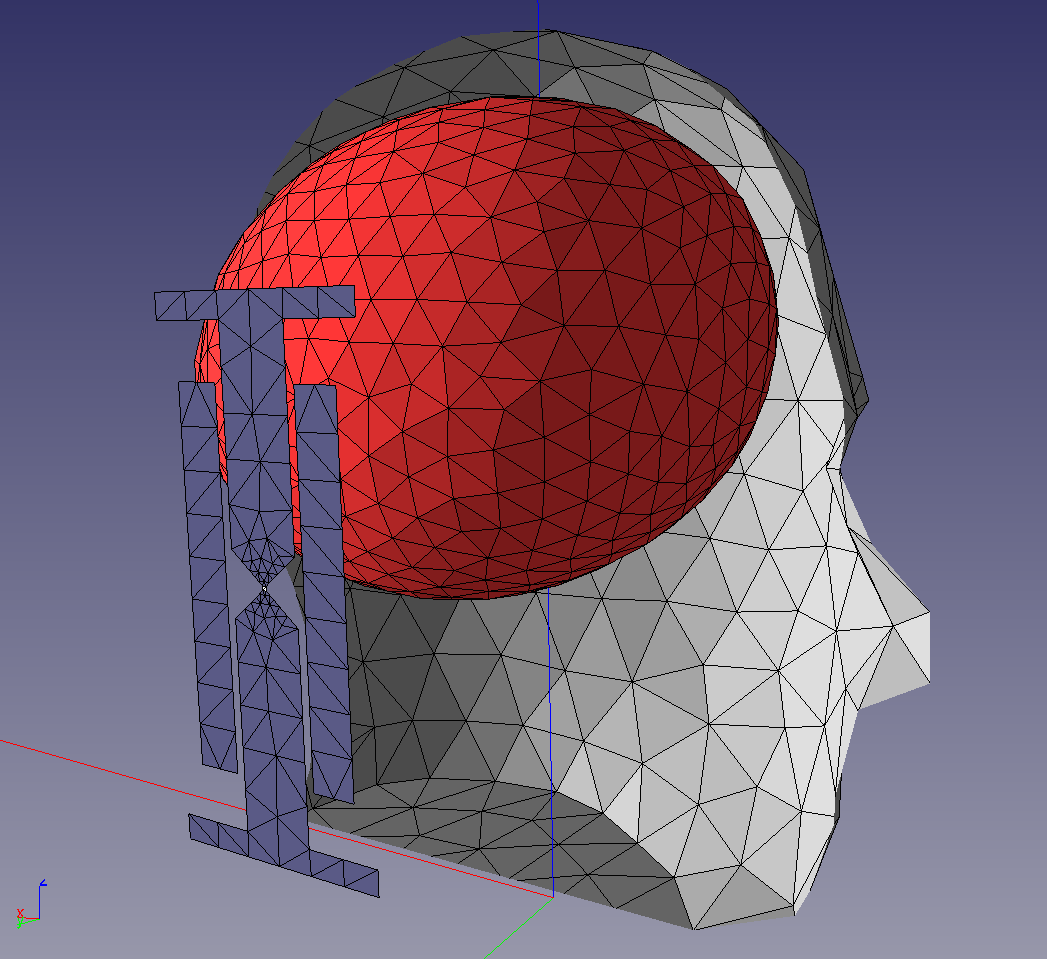
\includegraphics[
			width=0.7\linewidth,
			trim={0 0 0 0},clip]{scene_brain}
		}
		\\
		\subfloat[Zoom sur la zone d'injection du signal (en blanc).]{
			\label{img:tete_elposd_zoom}
		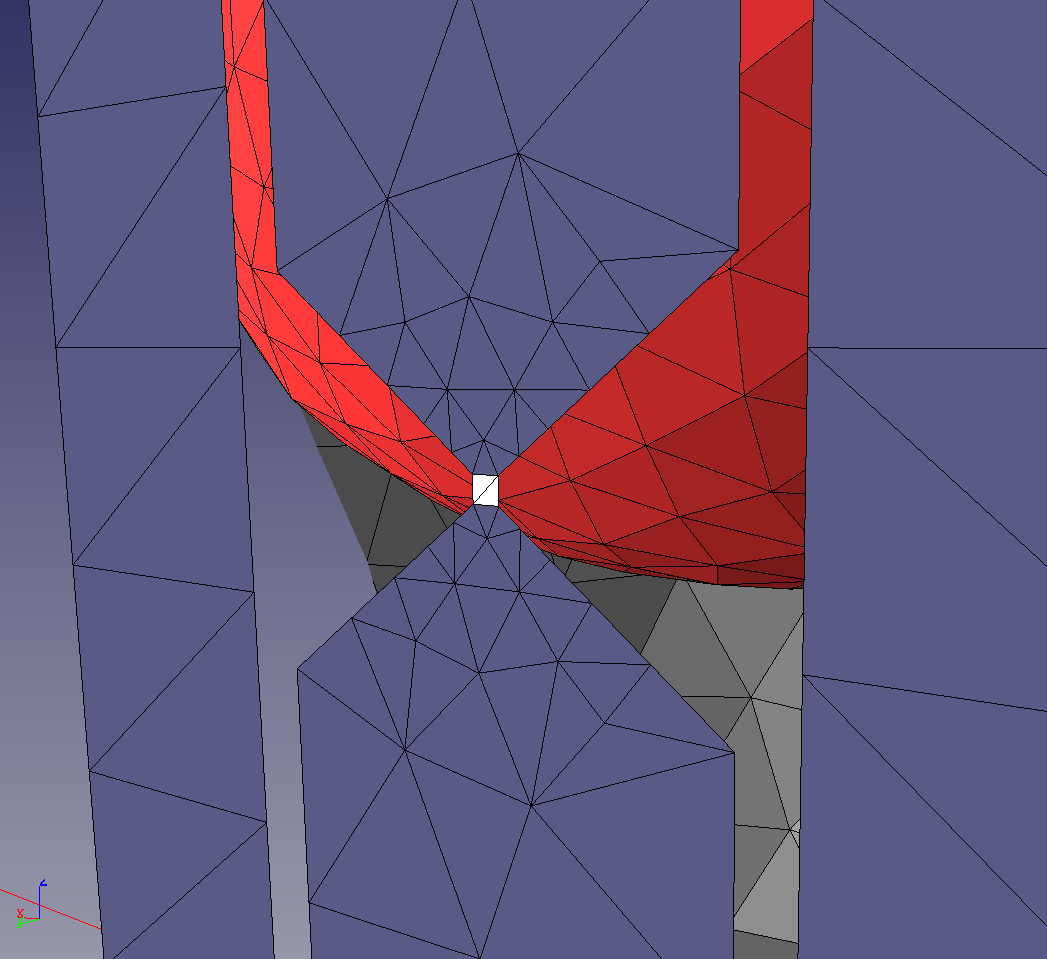
\includegraphics[
			width=0.7\linewidth,
			trim={0 200 0 200},clip]{scene_brain_zoom}
		}
	\end{center}
\end{figure}



\subsubsection{Matériaux}

Nous appliquons le modèle PEC (section \ref{ssect:PEC}) sur
toute la surface de l'antenne, hormis la source.
La source nous permet d'injecter le signal dans la scène.

La tête contient des matériaux diélectriques dont les propriétés sont données dans le tableau \ref{tab:proprietes_mat_tete}. Nous utilisons les propriétés
de la matière grise dans le cerveau simplifié et celles
de la matière osseuse dans le reste de la tête simplifiée \cite{Gabriel1}.
Les propriétés électromagnétiques de ces matériaux sont
globalement constantes sur la bande de fréquences utilisée ($0.1$ à $10$ GHz).


\begin{figure}[!h]
	\begin{center}
		\caption{
			\label{tab:proprietes_mat_tete}
			Propriétés électromagnétiques des matériaux utilisés
			dans la scène de la tête simplifiée.
		}
		
		\begin{tabular}{|c|c|c|c|c|}
			\hline
			Matériau & $\EPrm_r$ & $\HPrm_r$ & $\ECnd$ (S/m) & $\HCnd$ \\ \hline\hline
			cerveau & $51.8$ & $1$ & $1.521$ & $0$ \\	\hline
			os & $11.41$ & $1$ & $0.43$ & $0$ \\	\hline
			vide & $1$ & $1$ & $0$ & $0$ \\	\hline
		\end{tabular}
	\end{center}
\end{figure}



\subsubsection{Signal source}

Dans le cas de la méthode FDTD, la zone d'injection
du signal, représentée par un carré de côté $1$ mm
situé au centre de l'antenne,
est remplacée par un fil d'excitation de rayon $0.125$ mm.
Ce fil implémente un modèle dérivé de celui de Holland \textit{et al.} \cite{4091427}
et qui peut s'appliquer aux fils obliques \cite{guiffaut:hal-00624720}.

Dans le cas de notre solveur GD, nous utilisons
le modèle de générateur de Thévenin (section \ref{ssect:the_venin})
sur la zone d'injection.
Pour les deux méthodes, nous appliquons le modèle
d'excitation avec une impédance réelle de $50$ Ohms.
\\

Le signal que nous utilisons pour les deux méthodes
est une impulsion gaussienne modulée
définie sur l'intervalle $\PbTps$ par :
%\todo{être plus précis: donner le champ EM complet E=... H=..}
\begin{align} \label{eq:onde_plane_mod}
	g : t \mapsto A \sin \left( 2 \pi \freq_0 \left( t - t_A \right) \right) \exp \left( -\left( \frac{t - t_A}{\tau} \right)^2 \right) ,
\end{align}
avec $A$ l'amplitude de l'onde,
$\freq_0$ la fréquence centrale du signal,
$\tau$ donnant l'intervalle de temps entre les deux points de demie-amplitude
(de largeur $2 \sqrt{\ln 2} \tau$) de l'impulsion gaussienne non modulée
et $t_A$ l'antécédent de la valeur d'amplitude maximale
(figure \ref{img:onde_plane_mod}).
Ce signal modulé est le produit d'une impulsion gaussienne
\eqref{eq:onde_plane} avec une sinusoïde.

Dans le cas de notre solveur GD, ce signal est injecté
sur toute la zone d'injection par le champ électrique incident
(section \ref{ssect:the_venin}) :
\begin{align}
	\E_I = \frac{g(t)}{50} \frac{\overrightarrow{O\x_3}}{0.001}
	= 20 g(t) \overrightarrow{O\x_3}
\end{align}
avec une impédance de surface de $50$ Ohm définie sur
cette même surface.
Le champ magnétique incident est nul.


\begin{figure}[!h]
	\begin{center}
		\caption{
			\label{img:onde_plane_mod}
			Signal adimensionné de la tension générée, utilisé
			au cours des simulations avec l'antenne ELPOSD.
		}
		
		\begin{tikzpicture}[scale=1]
		\begin{axis}[
		axis lines=middle,
		xlabel=$ct$, x label style={at={(axis cs:3.3,0)},anchor=north},
		ylabel=$0$, y label style={at={(axis cs:0,-0.1)},anchor=east},
		xmin=-0.3,xmax=3.3,ymin=-1.1,ymax=1.1,
		xtick={0,1,...,4},%ytick={0,0.5,1},
		x post scale=1.8,
		y post scale=1.5,
		%legend style={at={(axis cs:0.9,0.2)},anchor=south west}
		]
		
		\addplot+[
		mark=none,
		color=gray,
		dotted, thick,
		samples=200,
		domain=0:3
		]
		{exp(-((x-1.448)/0.5509)^2)};
		
		\addplot+[
		thick,
		mark=none,
		color=red,
		samples=500,
		domain=0:3
		] table {gauss_mod.plt};
		%{exp(-((x-1.448)/0.5509)^2)*sin(2*3.14159*10/3*(x-1.448))};
		
		\node[anchor=east] (a) at (axis cs:0.9893456647,0.5){};
		\node[anchor=west] (b) at (axis cs:1.9066543353,0.5){};
		\draw[arrows={latex-latex}](a)--node[midway,below]{$2 \sqrt{\ln 2} \tau$}(b);
		
		\node[anchor=east] (c) at (axis cs:0,1){};
		\node[anchor=west] (d) at (axis cs:1.448,1){};
		\draw[dotted](c)--(d);
		
		\node[anchor=east] (e) at (axis cs:0,0.5){};
		\node[anchor=west] (f) at (axis cs:0.9893456647,0.5){};
		\draw[dotted](e)--(f);
		
		\node[anchor=north] (g) at (axis cs:1.448,0){};
		\node[anchor=south] (h) at (axis cs:1.448,1){};
		\draw[dotted](g)--(h);
		
		\node[anchor=north west] at (axis cs:1.448,0){$t_A$};
		\node[anchor=north west] at (axis cs:0,1){$A$};
		
		\end{axis}
		\end{tikzpicture}
	\end{center}
\end{figure}


Les paramètres $\tau$ et $t_A$ sont donnés par les relations suivantes :
\begin{subequations}
	\begin{align}
	\tau &= 2 \frac{\sqrt{- \ln (a_A)}}{\pi \Delta_\freq} ,
	\\
	t_A &= \tau \sqrt{- \ln (a_0)} ,
	\end{align}
\end{subequations}
où $a_0$ représente l'atténuation au temps initial ($t=0$),
$a_A$ représente l'atténuation au temps d'amplitude maximale $t_A$
et $\Delta_\freq$ représente la largeur de la bande de 
fréquences du signal considéré, centrée en $\freq_0$.

Pour notre cas d'application nous choisissons :
\begin{itemize}
	\item $A = 1$ ;
	\item $\freq_0 = 1$ GHz ;
	\item $\Delta_\freq = 0.6$ GHz ;
	\item $a_0 = 0.001$ (ou $0.1$ \%).
	\item $a_A = 0.05$ (ou $5$ \%) ;
\end{itemize}
Avec ces valeurs, dans le cas adimensionné,
nous avons $\tau \approx 0.5509$ et $t_A \approx 1.448$,
ce qui nous donne une durée de signal d'environ $10$ ns.


\subsubsection{Maillage}


La fréquence maximale considérée est de $\freq_{\max} =
\freq_0 + \Delta_\freq / 2 = 1.3$ GHz.
Le tableau \ref{tab:dx_mat_tete} présente la distance maximale
entre deux points d'interpolation 
selon la règle empirique du « $\lambda_{\min}$ sur $10$ »
en fonction des propriétés électromagnétiques des matériaux
à la fréquence $\freq_{\max} = 1.3$ GHz
(tableau~\ref{tab:proprietes_mat_tete}).


\begin{figure}[!h]
	\begin{center}
		\caption{
			\label{tab:dx_mat_tete}
			Distances maximales
			entre deux points d'interpolation
			en fonction des matériaux
			à la fréquence $1.3$ GHz.
		}
		
		\begin{tabular}{|c|c|c|}
			\hline
			Matériau & $\dx$ (mm) & $l_T$, $\Deg = 2$ (mm) \\ \hline\hline
			cerveau & $3.2$ & $12.8$ \\	\hline
			os & $6.8$ & $27.2$ \\	\hline
			vide & $23$ & $92$ \\	\hline
		\end{tabular}
	\end{center}
\end{figure}


Pour obtenir la taille d'arête maximale d'un hexaèdre à partir
de ces valeurs,
nous devons les multiplier par l'ordre d'interpolation spatiale choisi.
Dans le cas d'un maillage en tétraèdres, nous devons considérer
le double des arêtes des hexaèdres, afin d'appliquer le découpage
présenté en figure \ref{img:tetra_hexa}.

Pour une simulation à l'ordre d'interpolation spatiale $\Deg=2$,
nous maillons donc la scène avec les longueurs d'arête de tétraèdre $l_T$
données dans la dernière colonne du tableau \ref{tab:dx_mat_tete}.
Pour cela, nous commençons par mailler les surfaces avec la plus
petite taille d'arête à appliquer sur les volumes voisins
($12.8$ mm pour la peau du cerveau et $27.2$ pour la peau de la tête),
puis nous maillons les volumes.

L'antenne ELPOSD a préalablement été maillée avec une taille d'arête
maximale de $10$ mm afin d'assurer un rayonnement de bonne qualité.
Les champs électromagnétiques obtenus avec cette finesse de maillage correspondent
à ceux obtenus sur une version maillée à une taille d'arête maximale de $5$ mm
(figure \ref{img:rayonnement_elposd}) ainsi que ceux obtenus dans le cas de la méthode FDTD.
Dans le cas de l'antenne maillée à une taille d'arête maximale de $15$ mm,
nous observons une dégradation des résultats en fin de signal
(figure~\ref{img:rayonnement_elposd_zoom}).

\begin{figure}[!h]
	\begin{center}
		\caption{
			\label{img:rayonnement_elposd}
			Composante $\x_3$ du champ $\E$ au point
			$\Node{0}{0.095675}{0.12}$ (à mi-chemin de la distance
			antenne-oreille) dans une configuration « antenne seule ».
			Comparaison à la méthode FDTD pour différents raffinements de l'antenne
			dans le cas du schéma couplé GD-RK$2$.
		}
		
		\subfloat[Signal complet.]{
			\label{img:rayonnement_elposd_full}
		\begin{tikzpicture}[scale=1]
		\begin{axis}[
		axis lines=middle,
		xlabel=$t$ (ns),% x label style={at={(axis cs:0.5,0)},anchor=north},
		ylabel=$\E$ (V/m),% y label style={at={(axis cs:0,-0.05)},anchor=east},
		xmin=0,xmax=11,%ymin=-0.1,ymax=1.1,
		xtick={0,1,...,10},ytick={-6,-4,...,6},
		x post scale=1.8,
		y post scale=1.2,
		%legend style={at={(axis cs:0.9,0.2)},anchor=south west}
		]
		
		\addplot+[
		smooth,
		%thick,
		mark=none,
		color=red,
		] table
		{elposd/temsi_ez_p1.plt};
		\addlegendentry{Temsi @ $1$ mm}
		
		\addplot+[
		%thick,
		mark=none,
		color=blue,
		densely dashed,
		] table
		{elposd/teta_ez_p1_5mm.plt};
		\addlegendentry{Teta @ $5$ mm}
		
		\addplot+[
		%thick,
		mark=none,
		color=green,
		densely dotted,
		] table
		{elposd/teta_ez_p1_10mm.plt};
		\addlegendentry{Teta @ $10$ mm}
		
		\addplot+[
		%thick,
		mark=none,
		color=orange,
		densely dashdotted,
		] table
		{elposd/teta_ez_p1_15mm.plt};
		\addlegendentry{Teta @ $15$ mm}

		\end{axis}
		\end{tikzpicture}
		}
		\\
		\subfloat[Agrandissement de la zone d'intérêt.]{
			\label{img:rayonnement_elposd_zoom}
		\begin{tikzpicture}[scale=1]
		\begin{axis}[
		axis lines=middle,
		xlabel=$t$ (ns),% x label style={at={(axis cs:0.5,0)},anchor=north},
		ylabel=$\E$ (V/m),% y label style={at={(axis cs:0,-0.05)},anchor=east},
		xmin=7,xmax=10,ymin=-1.6,ymax=2.2,
		xtick={7,7.5,...,9.5},ytick={-1,-0.5,...,2},
		x post scale=1.8,
		y post scale=1.2,
		%legend style={at={(axis cs:0.9,0.2)},anchor=south west}
		]
		
		\addplot+[
		smooth,
		%thick,
		mark=none,
		color=red,
		] table
		{elposd/temsi_ez_p1.plt};
		\addlegendentry{Temsi @ $1$ mm}
		
		\addplot+[
		%thick,
		mark=none,
		color=blue,
		densely dashed,
		] table
		{elposd/teta_ez_p1_5mm.plt};
		\addlegendentry{Teta @ $5$ mm}
		
		\addplot+[
		%thick,
		mark=none,
		color=green,
		densely dotted,
		] table
		{elposd/teta_ez_p1_10mm.plt};
		\addlegendentry{Teta @ $10$ mm}
		
		\addplot+[
		%thick,
		mark=none,
		color=orange,
		densely dashdotted,
		] table
		{elposd/teta_ez_p1_15mm.plt};
		\addlegendentry{Teta @ $15$ mm}
		
		
		\end{axis}
		\end{tikzpicture}
		}
	\end{center}
\end{figure}

Après cette phase de maillage, nous obtenons un ensemble de $19413$ tétraèdres.
En résultent $77652$ hexaèdres quelconques après le découpage des tétraèdres,
auxquels s'ajoutent $4570$ hexaèdres droits en bordure de domaine pour
l'application du modèle PML.
Les surfaces présentées dans la figure \ref{img:tete_elposd}
sont issues de ce maillage.
\\

Dans le cas de la méthode FDTD, la zone d'injection
du signal, représentée par un carré de côté $1$ mm
situé au centre de l'antenne,
impose le pas de discrétisation.
Cette méthode de calcul nécessite de discrétiser la scène en mailles
hexaédriques sous la forme d'une grille structurée.
Le maillage résultant est composé d'environ $77.5$ millions de mailles
($417 \times 428 \times 434$).
Le modèle PML ajoute environ $12$ millions de mailles en bordure
de domaine.
Nous avons donc une grille structurée composée d'un peu moins de $90$ millions
de mailles de côté $1$ mm.
Soit un nombre de mailles $1087$ fois plus important que pour la méthode GD.
\\


\subsection{Comparaison à la méthode FDTD}
\label{ssect:tete_simplifiee_comp}

\subsubsection{Mémoire}
\label{sssect:tete_simplifiee_comp_mem}

Du point de vue de la mémoire, la simulation GD occupe $380$ Mo sur le GPU
(avec environ $100$ Mo supplémentaires pour l'allocation des instances OpenCL)
contre environ $9$ Go en RAM dans le cas de la simulation FDTD, soit
$23$ fois moins de mémoire utile pour la méthode GD.

Cette différence d'occupation en mémoire est principalement liée à la quantité de mailles
et aux degrés de liberté par maille. Dans le cas de la méthode GD,
la nature non structurée du maillage nécessite aussi de stocker une grande
quantité de coordonnées et d'informations de connectivité entre les mailles.


\subsubsection{Performances}
\label{sssect:tete_simplifiee_comp_perfs}

En temps de calcul, la simulation FDTD sur grille structurée a nécessité $4.85$ heures
pour simuler $20$ ns de temps physique sur $22$ cœurs (logiques) d'un processeur
Intel Dual Xeon E5645 ($2 \times 6$ cœurs physiques hyperthreadés) cadencé à $2.40$ GHz.
Le temps de calcul sur $46$ cœurs (logiques) du plus récent processeur Intel Dual Xeon E5-2650 v4
($2 \times 12$ cœurs physiques hyperthreadés) cadencé à $2.20$ GHz est de $2.24$ heures.
Le coefficient CFL imposé par la largeur du fil d'excitation est de $0.92$
et le pas de temps de la simulation est calculé à $1.772 \cdot 10^{-12}$ s
par la condition CFL classique utilisée avec la méthode FDTD.
\\


Dans le cas de la méthode GD sur maillage non structuré à l'ordre spatial $\Deg=2$,
la simulation a nécessité $1.88$ heures de
calcul sur un GPU NVidia GeForce GTX 1070 cadencé à $1.721$ GHz
et $1.19$ heures de
calcul sur un GPU NVidia GeForce GTX 1080 Ti cadencé à $1.582$ GHz.

L'application du diagnostic de la puissance itérée (section \ref{ssect:puissance itérée})
nous a permis de constater que dans le cas ce cette simulation, la condition
CFL de stabilité \eqref{eq:cfl1} sous-évalue le pas de temps de stabilité.
Nous avons fixé le coefficient CFL à $3.1$ et utilisé la formule \eqref{eq:cfl1}
pour le calcul du pas de temps de la simulation.
Le pas de temps ainsi obtenu est de $6.641 \cdot 10^{-14}$ s,
soit $27$ fois plus petit que celui utilisé dans le cas de la méthode FDTD.
\\

Les performances des deux solveurs peuvent donc être considérées du même ordre de grandeur
sur ce cas d'application.
Bien que la méthode GD soit présentée comme étant plus rapide que la méthode
FDTD, le temps de restitution est fonction du support de calcul utilisé.
Les temps de calculs obtenus sont résumés dans le tableau \ref{tab:tete_elposd_times}.

La méthode GD est très bien adaptée dans ce cas d'application compte tenu du
facteur d'échelle (proche de $100$) entre la plus petite et la plus grande maille du maillage. La méthode FDTD quant à elle, est directement affectée par la plus petite
maille qui impose le pas spatial de la grille structurée.


\begin{figure}[!h]
	\begin{center}
		\caption{
			\label{tab:tete_elposd_times}
			Temps de calcul des méthodes GD et FDTD en fonction
			du support d'exécution dans le cas de la simulation de
			l'antenne ELPOSD placée à proximité de la tête humaine simplifiée.
		}
		
		\begin{tabular}{|c|c|c|c|}
			\hline
			Solveur & Support d'exécution & CFL & Temps (h) \\ \hline\hline
			\multirow{2}{*}{Temsi} & Dual Xeon E5645, 22 threads & $0.92$ & $4.85$ \\	\cline{2-4}
			& Dual Xeon E5-2650 v4, 46 threads & $0.92$ & $\bm{2.24}$ \\	\hline
			\multirow{2}{*}{Teta} & GeForce GTX 1070 & $3.1$ & $1.88$ \\	\cline{2-4}
			& GeForce GTX 1080 Ti & $3.1$ & $\bm{1.19}$ \\	\hline
		\end{tabular}
	\end{center}
\end{figure}


\subsubsection{Résultats}
\label{sssect:tete_simplifiee_comp_res}

La figure \ref{img:tete_elposd_cutplane} présente un plan de coupe
des résultats de la simulation par la méthode GD.


\begin{figure}[!h]
	\begin{center}
		\caption{
			\label{img:tete_elposd_cutplane}
			Plan de coupe $(\x_1 O \x_2)$ en $\x_3 = 0.12$ m
			du logarithme (10dB) de la norme du champ électrique de la solution
			calculée dans le cas de la simulation de l'antenne ELPOSD
			placée à proximité de la tête humaine simplifiée
			au temps $t=3$ ns.
			Discrétisation à $5$ mm.
			La zone rouge correspond au centre de l'antenne, la zone
			bleue foncée correspond à la tête simplifiée.
		}
		
		\begin{tikzpicture}
		\begin{axis}[
		colormap/jet,
		colorbar,
		colorbar style={
			title={$\Norm{\E}$ (dBV/m)},
			%ylabel=Z-value,
			%ytick={0,0.2,0.4,0.6,0.8,1},
			%ymin=0,%ymax=2,
			%			yticklabel style={
			%				text width=2.5em,
			%				align=right,
			%				/pgf/number format/.cd,
			%				fixed,
			%				fixed zerofill
		},
		xlabel=$\x_1$, %x label style={at={(axis cs:1.15,0)},anchor=north},
		ylabel=$\x_2$, %y label style={at={(axis cs:0,-0.05)},anchor=east},	
		xtick={-0.2,-0.1,0,0.1,0.2},
		ytick={-0.2,-0.1,0,0.1,0.2},
		%tick label style={font=\tiny},
		view={0}{90},
		x post scale=1.4,
		y post scale=1.6,
		]

		\addplot3+[surf,%shader=interp,
		%patch type=rectangle,
		domain = -0.202285:0.212715,
		domain y = -0.205175:0.219825,
		mesh/rows=84,
		mesh/cols=86,
		] table[mark=none] {tete_elposd/teta_tete_elposd_xoy_t_3ns.plt};

%		\addplot3+[surf,%shader=interp,
%		%patch type=rectangle,
%		domain = -0.202285:0.213715,		
%		domain y = -0.205175:0.221825,		
%		mesh/rows=417,
%		mesh/cols=428,
%		] table[mark=none] {tete_elposd/teta_tete_elposd_xoy_t_3ns_1mm.plt};
		\end{axis}
		\end{tikzpicture}
	\end{center}
\end{figure}


Ces résultats sont très proches de ceux obtenus avec la méthode FDTD.
Afin de faciliter la comparaison, 
nous présentons aussi la valeur de la composante $\x_3$ du champ électrique
mesuré en différents points d'observation (figure \ref{img:tete_elposd_curves}) :
\begin{itemize}
	\item en $O_1 = \Node{0}{0.095675}{0.12}$, à mi-chemin entre l'antenne et la tête ;
	\item en $O_2 = \Node{0}{0}{0.12}$, à l'intérieur du cerveau, à hauteur de la zone
	source de l'antenne ;
	\item en $O_3 = \Node{0}{-0.113175}{0.12}$, le symétrique de la zone
	source de l'antenne par rapport au point $O_2$.
\end{itemize}


\begin{figure}[!h]
	\centering
		\caption{
			\label{img:tete_elposd_curves}
			Valeur de la composante $\x_3$ du champ électrique
			mesuré en différents points d'observation dans le cas de la simulation de
			l'antenne ELPOSD placée à proximité de la tête humaine simplifiée.
			Comparaison de la méthode FDTD au schéma couplé GD-RK$2$.
		}

		\subfloat[Au point $O_1$.]{
			\centering
			\label{img:tete_elposd_curves_O1}
			\begin{tikzpicture}[scale=0.8]
			\begin{axis}[
			axis lines=middle,
			xlabel=$t$ (ns), x label style={at={(axis cs:11.5,0)},anchor=south},
			ylabel=$\E$ (V/m), y label style={at={(axis cs:0,6)},anchor=west},
			xmin=0,xmax=13,%ymin=-0.1,ymax=1.1,
			xtick={0,2,...,12},%ytick={0,0.5,1},
			%x post scale=1.8,
			%y post scale=1.2,
			%legend style={at={(axis cs:0.9,0.2)},anchor=south west}
			]
			
			\addplot+[
			%thick,
			mark=none,
			color=red,
			] table
			[y expr=-\thisrowno{1}]
			{tete_elposd/temsi_ez_O1.plt};
			%\addlegendentry{Temsi}
			
			\addplot+[
			%thick,
			mark=none,
			color=blue,
			densely dashed,
			] table
			{tete_elposd/teta_ez_O1.plt};
			%\addlegendentry{Teta}
			
			\end{axis}
			\end{tikzpicture}
		}
		\hfill
		\subfloat[Au point $O_2$.]{
			\centering
			\label{img:tete_elposd_curves_O2}
			\begin{tikzpicture}[scale=0.8]
			\begin{axis}[
			axis lines=middle,
			xlabel=$t$ (ns), x label style={at={(axis cs:11.5,0)},anchor=south},
			ylabel=$\E$ (V/m), y label style={at={(axis cs:0,0.175)},anchor=west},
			xmin=0,xmax=13,%ymin=-0.1,ymax=1.1,
			xtick={0,2,...,12},%ytick={0,0.5,1},
			%x post scale=1.8,
			%y post scale=1.2,
			%legend style={at={(axis cs:0.9,0.2)},anchor=south west}
			]
			
			\addplot+[
			%thick,
			mark=none,
			color=red,
			] table
			[y expr=-\thisrowno{1}]
			{tete_elposd/temsi_ez_O2.plt};
			\addlegendentry{Temsi}
			
			\addplot+[
			%thick,
			mark=none,
			color=blue,
			densely dashed,
			] table
			{tete_elposd/teta_ez_O2.plt};
			\addlegendentry{Teta}
			
			\end{axis}
			\end{tikzpicture}

		}	
		\\
		\subfloat[Au point $O_3$.]{
			\centering
			\label{img:tete_elposd_curves_O3}
			\begin{tikzpicture}[scale=0.8]
			\begin{axis}[
			axis lines=middle,
			xlabel=$t$ (ns), x label style={at={(axis cs:11.5,0)},anchor=south},
			ylabel=$\E$ (mV/m), y label style={at={(axis cs:0,70)},anchor=west},
			xmin=0,xmax=13,%ymin=-0.1,ymax=1.1,
			xtick={0,2,...,12},%ytick={0,0.5,1},
			%x post scale=1.8,
			%y post scale=1.2,
			%legend style={at={(axis cs:0.9,0.2)},anchor=south west}
			]
			
			\addplot+[
			%thick,
			mark=none,
			color=red,
			] table
			[y expr=-\thisrowno{1}*1000]
			{tete_elposd/temsi_ez_O3.plt};
			%\addlegendentry{Temsi}
			
			\addplot+[
			%thick,
			mark=none,
			color=blue,
			densely dashed,
			] table
			[y expr=\thisrowno{1}*1000]
			{tete_elposd/teta_ez_O3.plt};
			%\addlegendentry{Teta}
			
			\end{axis}
			\end{tikzpicture}
		}	
		\hfill
		\subfloat[Position des points.]{
			\centering
			\label{img:tete_elposd_curves_pos}
			\begin{tikzpicture}[scale=4.8]
			\fill[white] (-0.2,0) rectangle (1.2,1);
			\draw (0,0) rectangle (1,1);
			\fill (0.14,0.45) rectangle (0.16,0.55);
			\draw[thick,fill=gray!20] (0.55,0.5) ellipse (0.25 and 0.35);
			\draw[thick,fill=gray!30] (0.55,0.55) ellipse (0.18 and 0.2);
			\draw (0.15,1) node[below] {SRC};
			\draw (0.55,1) node[below] {TETE};
			\draw[arrows={-latex}] (0.95,0.05) -- (0.95,0.15) node[above] {$\x_1$};
			\draw[arrows={-latex}] (0.95,0.05) -- (0.85,0.05) node[left] {$\x_2$};
			\fill[red] (0.23,0.5) circle (0.015) node[above,red]{$O_1$};
			\fill[red] (0.55,0.5) circle (0.015) node[above,red]{$O_2$};
			\fill[red] (0.94,0.5) circle (0.015) node[above,red]{$O_3$};
			\end{tikzpicture}
		}	
\end{figure}

Nous constatons que les deux solveurs produisent sensiblement les mêmes
résultats. Un léger décalage peut être constaté dans le cas des
mesures effectuées à l'intérieur du cerveau et de l'autre côté de la tête
par rapport à l'antenne.
Entre la tête et l'antenne, les résultats sont identiques.

Nous pouvons aussi remarquer que l'onde électromagnétique atteint le côté opposé
de la tête avant le centre du cerveau. Ces résultats sont dûs à la forte permittivité
des matériaux de la tête qui diminuent la vitesse de propagation des ondes.
Cette propriété des matériaux génère le phénomène d'« enroulement »
des ondes constaté au niveau de la zone du cerveau sur la figure \ref{img:tete_elposd_cutplane}.
\\

Nous avons évoqué d'autres axes d'optimisation dans les chapitres précédents.
Du point du vue de la discrétisation spatiale, nous pouvons réduire la masse
de calculs en appliquant l'ordre spatial adaptatif.
Nous avons aussi décrit une méthode d'intégration avec application d'un pas de temps
local par maille.
Les résultats et perfomances obtenues avec ces deux méthodes sont
présentés dans les sections suivantes.



\subsection{Application de l'ordre spatial adaptatif}
\label{ssect:tete_simplifiee_adaptatif}

Le découpage des tétraèdres génère des hexaèdres dont la taille $\min l_H$
de la plus petite arête peut être jusqu'à $6$ fois inférieure à la taille
donnée par l'application de la règle du « $\lambda_{\min}$ sur $10$ »
(tableau \ref{tab:comp_struct_nstruct_aretes}).
Nous pouvons donc appliquer un ordre
d'interpolation spatiale inférieur sur ces mailles (section~\ref{sect:ordre_adaptatif})
tout en conservant
un raffinement suffisant du point de vue de l'évaluation du pas de temps
de simulation (application du critère CFL \eqref{eq:cfl1} sur la plus petite
arête de chaque maille devant respecter la règle du « $\lambda_{\min}$ sur $10$ »).

Rappelons que nous imposons un ordre spatial minimal à $\Deg=1$. Ainsi,
la plupart des mailles de notre simulation passent à cet ordre d'interpolation.
Seuls les hexaèdres droits générés en bordure de domaine pour l'application du modèle PML
ont une taille suffisante pour conserver un ordre spatial $2$.
Du point de vue de la discrétisation spatiale (théorème de Shannon
sur l'échantillonnage des signaux),
le passage de l'ordre $2$ à l'ordre $1$ implique une discrétisation
proche de « $\lambda_{\min}$ sur $5$ » à proximité des arêtes les plus longues.
Cet échantillonnage est suffisant pour représenter fidèlement les ondes.

Le maillage ainsi que les paramètres de simulation (hormis les ordres d'interpolation)
sont identiques à ceux présentés dans la section \ref{ssect:tete_simplifiee_desc}.
Nous obtenons donc une simulation composée de $77652$ hexaèdres quelconques
spatialement interpolés à l'ordre $1$ et $4570$ hexaèdres droits en bordure de domaine
pour l'application du modèle PML interpolés à l'ordre $2$.


\subsubsection{Performances}

Cette simulation a duré $0.31$ heures sur NVidia GeForce GTX 1080 Ti
avec l'application du coefficient CFL $4.5$ déterminé par la méthode de la puissance
itérée pour l'ordre d'interpolation spatiale $\Deg=1$.
Les mailles du modèle PML sont suffisamment grandes pour être stables
avec ce coefficient CFL.
Le pas de temps de la simulation est de $1.446 \cdot 10^{-13}$ s.

Une accélération d'un facteur $3.8$
par rapport à la même simulation interpolant spatialement à l'ordre
$\Deg=2$ sur toutes les mailles est donc constaté.


\subsubsection{Résultats}

Les résultats sont proches de ceux obtenus avec une interpolation
homogène à l'ordre $2$.
Nous constatons cependant une légère
perte dans l'amplitude du signal ($-5$ \%), dès son injection
via le modèle de générateur de Thévenin (section \ref{ssect:the_venin}).

L'amplitude du signal au niveau du point de mesure $O_3$,
situé de l'autre côté de la tête, est plus faible que celle
mesurée pour l'ordre $2$. Ceci témoigne du fait que l'interpolation
spatiale à l'ordre $1$ est plus dissipative qu'une interpolation à l'ordre $2$.
En effet, nous passons de fonctions de base quadratiques à des fonctions linéaires,
l'approximation est donc moins précise.
L'amplitude du signal au niveau du point de mesure $O_2$,
situé dans le cerveau, est quant à elle plus importante 
que celle mesurée pour l'ordre $2$.

Toutefois, mises à part les différences d'amplitude, la forme du signal est fidèle
au signal mesuré pour une interpolation à l'ordre $2$.
La perte de précision est naturellement induite par l'utilisation d'un ordre
d'interpolation inférieur, et spécialement dans le cas de l'ordre $1$
qui linéarise (par morceaux) l'approximation de la solution.
Il est donc préférable d'appliquer l'ordre adaptatif dans le cas
d'une interpolation initiale d'ordre plus élevé.
\\

\begin{figure}[!h]
	\centering
	\caption{
		\label{img:tete_elposd_adapt_curves}
		Valeur de la composante $\x_3$ du champ électrique
		mesuré en différents points d'observation dans le cas de la simulation de
		l'antenne ELPOSD placée à proximité de la tête humaine simplifiée.
		Comparaison du schéma couplé GD-RK$2$ pour $\Deg=2$ au même schéma
		avec application de l'ordre d'interpolation spatiale adaptatif ($d\le2$).
	}
	
	\subfloat[Au point $O_1$.]{
		\centering
		\label{img:tete_elposd_adapt_curves_O1}
		\begin{tikzpicture}[scale=0.8]
		\begin{axis}[
		axis lines=middle,
		xlabel=$t$ (ns), x label style={at={(axis cs:11.5,0)},anchor=south},
		ylabel=$\E$ (V/m), y label style={at={(axis cs:0,6)},anchor=west},
		xmin=0,xmax=13,%ymin=-0.1,ymax=1.1,
		xtick={0,2,...,12},%ytick={0,0.5,1},
		%x post scale=1.8,
		%y post scale=1.2,
		%legend style={at={(axis cs:0.9,0.2)},anchor=south west}
		]
		
		\addplot+[
		%thick,
		mark=none,
		color=red,
		] table
		{tete_elposd/teta_ez_O1.plt};
		%\addlegendentry{Temsi}
		
		\addplot+[
		%thick,
		mark=none,
		color=blue,
		densely dashed,
		] table
		{tete_elposd/teta_ez_O1_adapt.plt};
		%\addlegendentry{Teta}
		
		\end{axis}
		\end{tikzpicture}
	}
	\hfill
	\subfloat[Au point $O_2$.]{
		\centering
		\label{img:tete_elposd_adapt_curves_O2}
		\begin{tikzpicture}[scale=0.8]
		\begin{axis}[
		axis lines=middle,
		xlabel=$t$ (ns), x label style={at={(axis cs:11.5,0)},anchor=south},
		ylabel=$\E$ (V/m), y label style={at={(axis cs:0,0.175)},anchor=west},
		xmin=0,xmax=13,%ymin=-0.1,ymax=1.1,
		xtick={0,2,...,12},%ytick={0,0.5,1},
		%x post scale=1.8,
		%y post scale=1.2,
		%legend style={at={(axis cs:0.9,0.2)},anchor=south west}
		]
		
		\addplot+[
		%thick,
		mark=none,
		color=red,
		] table
		{tete_elposd/teta_ez_O2.plt};
		\addlegendentry{$\Deg=2$}
		
		\addplot+[
		%thick,
		mark=none,
		color=blue,
		densely dashed,
		] table
		{tete_elposd/teta_ez_O2_adapt.plt};
		\addlegendentry{$d\le2$}
		
		\end{axis}
		\end{tikzpicture}
		
	}	
	\\
	\subfloat[Au point $O_3$.]{
		\centering
		\label{img:tete_elposd_adapt_curves_O3}
		\begin{tikzpicture}[scale=0.8]
		\begin{axis}[
		axis lines=middle,
		xlabel=$t$ (ns), x label style={at={(axis cs:11.5,0)},anchor=south},
		ylabel=$\E$ (mV/m), y label style={at={(axis cs:0,70)},anchor=west},
		xmin=0,xmax=13,%ymin=-0.1,ymax=1.1,
		xtick={0,2,...,12},%ytick={0,0.5,1},
		%x post scale=1.8,
		%y post scale=1.2,
		%legend style={at={(axis cs:0.9,0.2)},anchor=south west}
		]
		
		\addplot+[
		%thick,
		mark=none,
		color=red,
		] table
		[y expr=\thisrowno{1}*1000]
		{tete_elposd/teta_ez_O3.plt};
		
		\addplot+[
		%thick,
		mark=none,
		color=blue,
		densely dashed,
		] table
		[y expr=\thisrowno{1}*1000]
		{tete_elposd/teta_ez_O3_adapt.plt};
		
		\end{axis}
		\end{tikzpicture}
	}	
	\hfill
	\subfloat[Position des points.]{
		\centering
		\label{img:tete_elposd_adapt_curves_pos}
		\begin{tikzpicture}[scale=4.8]
		\fill[white] (-0.2,0) rectangle (1.2,1);
		\draw (0,0) rectangle (1,1);
		\fill (0.14,0.45) rectangle (0.16,0.55);
		\draw[thick,fill=gray!20] (0.55,0.5) ellipse (0.25 and 0.35);
		\draw[thick,fill=gray!30] (0.55,0.55) ellipse (0.18 and 0.2);
		\draw (0.15,1) node[below] {SRC};
		\draw (0.55,1) node[below] {TETE};
		\draw[arrows={-latex}] (0.95,0.05) -- (0.95,0.15) node[above] {$\x_1$};
		\draw[arrows={-latex}] (0.95,0.05) -- (0.85,0.05) node[left] {$\x_2$};
		\fill[red] (0.23,0.5) circle (0.015) node[above,red]{$O_1$};
		\fill[red] (0.55,0.5) circle (0.015) node[above,red]{$O_2$};
		\fill[red] (0.94,0.5) circle (0.015) node[above,red]{$O_3$};
		\end{tikzpicture}
	}	
\end{figure}



\subsection{Application du schéma LRK2}
\label{ssect:tete_simplifiee_lrk2}

Avant d'appliquer la méthode à pas de temps local, nous commençons par appliquer
le schéma LRK$2$ décrit dans la section \ref{sect:pas de temps local lrk2}.
Rappelons qu'il s'agit du schéma RK$2$ modifié pour effectuer
une prédiction locale à chaque maille. L'étape de mise-à-jour reste inchangée.
Le pas de temps de simulation est homogène
sur tout le maillage et nous reprenons la condition CFL \eqref{eq:cfl1}.

Le coefficient CFL de ce schéma, déterminé par la méthode de la puissance
itérée pour l'ordre d'interpolation spatiale $\Deg=2$, est de $1.9$.
La stabilité de ce schéma est donc inférieure au schéma RK$2$.
Le pas de temps de la simulation est de $4.071 \cdot 10^{-14}$ s
et le temps de calcul sur NVidia GeForce GTX 1080 Ti est de $1.71$ heures.

Les résultats avec l'application de ce schéma sont équivalents à ceux obtenus
avec le schéma RK$2$, malgré l'utilisation d'un prédicteur local.
Cependant, cette méthode est $1.44$ fois moins efficace
compte tenu de son coefficient CFL de stabilité.
Remarquons tout de même qu'à pas de temps égal, ce schéma serait plus efficace
que le schéma RK$2$ de $12$ \%, cela grâce aux propiétés locales du terme de flux
de l'étape de prédiction.
\\


\subsection{Application du schéma LTS2}
\label{ssect:tete_simplifiee_dt_local}


Contrairement à une méthode à pas de temps homogène telle que
les méthodes de type RK (section \ref{ssect:rk}), le schéma LTS$2$ impose
de vérifier un critère de type CFL sur chaque maille.
Dans le cas d'une méthode à pas de temps homogène,
il suffit de satisfaire
la condition CFL sur la maille la plus
contraignante (généralement une seule maille : la plus petite, ou
dans certains cas une maille très déformée).

Une condition CFL de stabilité offrant les meilleurs performances
est donc difficile à déterminer. En effet, dans le cas d'une une grande
maille (déformée) sur laquelle le schéma en temps homogène était stable avec
le pas de temps imposé par la plus petite maille du maillage,
des instabilités peuvent apparaitre lors de l'utilisation d'un pas de
temps (calculé avec la même condition CFL) propre à chaque maille.

Nous présentons donc des résultats pour les coefficients CFL
de stabilité maximaux dans le cas de l'application des critères
CFL \eqref{eq:cfl1} et \eqref{eq:cfl2}.
Nous noterons respectivement ces critères CFL$1$ et CFL$2$.
Pour le second critère, nous avons testé différentes valeurs pour l'exposant $\alpha$.
Ce paramètre permet de faire varier le gradient de la fonction
qui associe à chaque maille son pas de temps et impacte directement
la répartition des classes de pas de temps qui utilise la fonction $\log_2$.
\\

Nous utilisons le schéma LTS$2$ sur le cas d'application de
l'antenne dipolaire placée à proximité d'une tête humaine simplifiée
(section \ref{ssect:tete_simplifiee_desc}).
Nous choisissons l'ordre d'interpolation spatiale $\Deg = 1$ et
remplaçons la condition de bord PML par la condition de
Silver-Müller (section \ref{ssect:silver_mueller}).
Dans ces conditions, la simulation à l'aide du schéma couplé GD-RK$2$
sur $20$ ns de temps physique a nécessité $0.44$ heures de calcul
sur un GPU NVidia GeForce GTX 1070.
Le pas de temps de cette simulation est de $1.446 \cdot 10^{-13}$ s
déterminé à l'aide du critère CFL \eqref{eq:cfl1}.
Le coefficient CFL de stabilité déterminé par la méthode
de la puissance itérée (section \ref{ssect:puissance itérée})
est de $4.5$.


\subsubsection{Mémoire}

Du point de vue de la mémoire, la simulation GD-RK$2$ occupe $142$ Mo sur le
GPU contre en moyenne $155$ Mo dans le cas des simulations GD-LTS$2$,
soit environ $10$ \% de plus de mémoire utile pour le schéma LTS$2$.

Cette faible différence d'occupation en mémoire est principalement liée à la
génération d'interfaces supplémentaires entre les classes de pas de temps
et les zones de mailles tampon.
En effet, l'implémentation actuelle de ce schéma utilise le découpage en zones homogènes
pour séparer les classes de pas de temps et les mailles tampon.


\subsubsection{Performances}


Les performances en dimension $3$ sont nettement inférieures à celles constatées en
dimension $1$ (section \ref{sect:pas de temps local transport}).
En effet, en dimension $1$, une interface (terme de flux) entre $2$ classes de pas de
temps ne représente qu'un seul degré de liberté contre des milliers en dimension $3$.
Ces interfaces sont des surfaces fermées topologiquement comparables à des
frontières de boules.

Dans le cas de la simulation à pas de temps homogène, toutes les mailles
sont regroupées en une unique zone homogène.
Les kernels de calcul sont donc peu nombreux et traitent un grand nombre
de mailles.
Dans le cas des simulations à pas de temps local, nous avons entre $6$ et $16$
zones homogènes supplémentaires, issues du découpage en classes de pas de temps.
Ce découpage multiplie d'autant le nombre de kernels exécutés et génère
une interface entre chacune de ces zones (agencement en « peau d'oignon »).
Ces zones et interfaces comptent un nombre de mailles réduit, les kernels sont donc
moins efficaces, en plus d'augmenter le temps de latence OpenCL
par leur nombre.

Néanmoins, malgré tous ces facteurs diminuant l'efficacité
en OpenCL et dimension $3$, nous avons obtenu
de meilleures performances en temps de calcul à l'aide du schéma LTS$2$.
Le tableau \ref{tab:lts2_perfs} présente les résultats en temps de calcul
en fonction du critère et du coefficient de CFL.

\begin{figure}[!h]
	\centering
	\caption{
		\label{tab:lts2_perfs}
		Temps de calcul des méthodes RK$2$ et LTS$2$ en fonction
		du critère et du coefficient de CFL sur GPU NVidia GeForce GTX 1070
		dans le cas de la simulation de l'antenne ELPOSD
		placée à proximité de la tête humaine simplifiée
		pour l'ordre d'interpolation spatiale $\Deg = 1$.
		La dernière ligne correspond au temps de calcul obtenu en prenant pour chaque
		maille le plus grand pas de temps donné par tous les critères CFL précédents.
		}
		
	\begin{tabular}{|c|c|c|c|c|c|c|}
		\hline
		\multirow{2}{*}{Méthode} & \multicolumn{3}{c|}{CFL} & \multirow{2}{*}{$\dt_{\min}^l$ (s)} & \multirow{2}{*}{$N_t$} & \multirow{2}{*}{$T_\mathrm{s}$ (h)} \\	\cline{2-4}
		& crit. & $\alpha$ & coeff. & & & \\	\hline\hline
		RK$2$ & $1$ & - & $4.5$ & $1.446 \cdot 10^{-13}$ & $0$ & $0.44$ \\ \hline
		\multirow{8}{*}{LTS$2$} & $1$ & - & $0.22$ & $7.070 \cdot 10^{-15}$ & $7$ & $1.10$ \\ \cline{2-7}
		& \multirow{6}{*}{$2$} & $4/3$ & $1.2 \cdot 10^{3}$ & $3.285 \cdot 10^{-15}$ & $8$ & $2.21$ \\ \cline{3-7}
		& & $1$ & $0.20$ & $8.601 \cdot 10^{-15}$ & $7$ & $0.96$ \\ \cline{3-7}
		& & $3/4$ & $3.2 \cdot 10^{-4}$ & $1.931 \cdot 10^{-14}$ & $6$ & $0.54$ \\ \cline{3-7}
		& & $2/3$ & $3.1 \cdot 10^{-5}$ & $2.094 \cdot 10^{-14}$ & $5$ & $0.50$ \\ \cline{3-7}
		& & $1/2$ & $4.5 \cdot 10^{-7}$ & $3.894 \cdot 10^{-14}$ & $4$ & $0.39$ \\ \cline{3-7}
		& & $1/4$ & $6.5 \cdot 10^{-10}$ & $7.721 \cdot 10^{-14}$ & $3$ & $0.33$ \\ \cline{2-7}
		& \multicolumn{3}{c|}{$\max \dt$} & $7.721 \cdot 10^{-14}$ & $4$ & $0.28$ \\ \hline
	\end{tabular}
\end{figure}


\begin{figure}[!h]
	\centering
	\caption{
		\label{tab:lts2_classes}
		Composition des zones homogènes pour les méthodes RK$2$ et LTS$2$ en fonction
		du critère et du coefficient de CFL
		dans le cas de la simulation de l'antenne ELPOSD
		placée à proximité de la tête humaine simplifiée
		pour l'ordre d'interpolation spatiale $\Deg = 1$.
	}
	
	\subfloat[Zones homogènes.]{
		\label{tab:lts2_classes_zones}
	\resizebox{0.85\linewidth}{!}{%
	\begin{tabular}{|c|c|c|c|c|c|c|c|c|c|}
		\hline
		\textbf{Méthode} & RK$2$ & \multicolumn{8}{c|}{LTS$2$} \\	\hline
		\textbf{CFL}[-$\alpha$] & $1$ & $1$ & $2$-$4/3$ & $2$-$1$ & $2$-$3/4$ & $2$-$2/3$ & $2$-$1/2$ & $2$-$1/4$ & $\max \dt$ \\	\hline\hline
		$N_t$ & $0$ & $7$ & $8$ & $7$ & $6$ & $5$ & $4$ & $3$ & $4$ \\ \hline\hline
		$\#\mathcal{C}_0$ \eqref{eq:lts2_classes} & $77652$ & $640$ & $601$ & $649$ & $799$ & $876$ & $1063$ & $4741$ & $4560$ \\	\hline
		$\#\mathcal{T}_0$ \eqref{eq:lts2_tampon} & - & $608$ & $592$ & $660$ & $593$ & $540$ & $527$ & $1552$ & $1603$ \\	\hline
		$\#\mathcal{C}_1\setminus\mathcal{T}_0$ & - & $1036$ & $1035$ & $975$ & $1289$ & $1422$ & $3239$ & $21551$ & $2414$ \\	\hline
		$\#\mathcal{T}_1$ & - & $984$ & $1016$ & $984$ & $1113$ & $1099$ & $1504$ & $2056$ & $2178$ \\	\hline
		$\#\mathcal{C}_2\setminus\mathcal{T}_1$ & - & $1156$ & $1128$ & $1167$ & $1749$ & $2812$ & $11063$ & $11169$ & $9941$ \\	\hline
		$\#\mathcal{T}_2$ & - & $1088$ & $1068$ & $1093$ & $1269$ & $1443$ & $4548$ & $5499$ & $11074$ \\	\hline
		$\#\mathcal{C}_3\setminus\mathcal{T}_2$ & - & $1208$ & $1065$ & $1262$ & $4843$ & $9403$ & $17074$ & $31084$ & $39058$ \\	\hline
		$\#\mathcal{T}_3$ & - & $1036$ & $924$ & $1045$ & $4352$ & $4682$ & $6204$ & - & $6608$ \\	\hline
		$\#\mathcal{C}_4\setminus\mathcal{T}_3$ & - & $1704$ & $833$ & $1779$ & $20045$ & $18492$ & $32430$ & - & $216$ \\	\hline
		$\#\mathcal{T}_4$ & - & $2224$ & $895$ & $2331$ & $7332$ & $5573$ & - & - & - \\	\hline
		$\#\mathcal{C}_5\setminus\mathcal{T}_4$ & - & $9888$ & $1147$ & $10259$ & $30144$ & $31310$ & - & - & - \\	\hline
		$\#\mathcal{T}_5$ & - & $9828$ & $1448$ & $10331$ & $4108$ & - & - & - & - \\	\hline
		$\#\mathcal{C}_6\setminus\mathcal{T}_5$ & - & $33384$ & $3455$ & $36614$ & $16$ & - & - & - & - \\	\hline
		$\#\mathcal{T}_6$ & - & $12476$ & $5734$ & $8443$ & - & - & - & - & - \\	\hline
		$\#\mathcal{C}_7\setminus\mathcal{T}_6$ & - & $392$ & $15980$ & $60$ & - & - & - & - & - \\	\hline
		$\#\mathcal{T}_7$ & - & - & $17203$ & - & - & - & - & - & - \\	\hline
		$\#\mathcal{C}_8\setminus\mathcal{T}_7$ & - & - & $23528$ & - & - & - & - & - & - \\	\hline
	\end{tabular}}
	}
	\\
	\subfloat[Interfaces.]{
		\label{tab:lts2_classes_interfaces}
	\resizebox{0.85\linewidth}{!}{%
	\begin{tabular}{|c|c|c|c|c|c|c|c|c|c|}
		\hline
		\textbf{Méthode} & RK$2$ & \multicolumn{8}{c|}{LTS$2$} \\	\hline
		\textbf{CFL}[-$\alpha$] & $1$ & $1$ & $2$-$4/3$ & $2$-$1$ & $2$-$3/4$ & $2$-$2/3$ & $2$-$1/2$ & $2$-$1/4$ & $\max \dt$ \\	\hline\hline
		$N_t$ & $0$ & $7$ & $8$ & $7$ & $6$ & $5$ & $4$ & $3$ & $4$ \\ \hline\hline
		$\#\mathcal{I}_0$ \eqref{eq:lts2_interfaces} & - & $570$ & $570$ & $580$ & $544$ & $486$ & $464$ & $1428$ & $1474$ \\	\hline
		$\#\Adh{\mathcal{T}_0} \cap \Adh{\mathcal{C}_1\setminus\mathcal{T}_0}$ & - & $582$ & $610$ & $544$ & $486$ & $474$ & $464$ & $1176$ & $1202$ \\	\hline
		$\#\mathcal{I}_1$ & - & $858$ & $900$ & $858$ & $992$ & $972$ & $1356$ & $1560$ & $1802$ \\	\hline
		$\#\Adh{\mathcal{T}_1} \cap \Adh{\mathcal{C}_2\setminus\mathcal{T}_1}$
		& - & $936$ & $966$ & $936$ & $1004$ & $992$ & $1152$ & $3168$ & $2584$ \\	\hline
		$\#\mathcal{I}_2$
		& - & $972$ & $966$ & $976$ & $1132$ & $1276$ & $3796$ & $4298$ & $9278$ \\	\hline
		$\#\Adh{\mathcal{T}_2} \cap \Adh{\mathcal{C}_3\setminus\mathcal{T}_2}$
		& - & $996$ & $1026$ & $1030$ & $1088$ & $1294$ & $5456$ & $5772$ & $9148$ \\	\hline
		$\#\mathcal{I}_3$
		& - & $978$ & $906$ & $1006$ & $3570$ & $3936$ & $5222$ & - & $7649$ \\	\hline
		$\#\Adh{\mathcal{T}_3} \cap \Adh{\mathcal{C}_4\setminus\mathcal{T}_3}$
		& - & $888$ & $790$ & $922$ & $4800$ & $5532$ & $6426$ & - & $309$ \\	\hline
		$\#\mathcal{I}_4$
		& - & $1872$ & $856$ & $2040$ & $6542$ & $4430$ & - & - & - \\	\hline
		$\#\Adh{\mathcal{T}_4} \cap \Adh{\mathcal{C}_5\setminus\mathcal{T}_4}$
		& - & $2910$ & $1002$ & $3048$ & $6654$ & $6270$ & - & - & - \\	\hline
		$\#\mathcal{I}_5$
		& - & $8172$ & $1326$ & $8522$ & $4998$ & - & - & - & - \\	\hline
		$\#\Adh{\mathcal{T}_5} \cap \Adh{\mathcal{C}_6\setminus\mathcal{T}_5}$
		& - & $9132$ & $1820$ & $9434$ & $24$ & - & - & - & - \\	\hline
		$\#\mathcal{I}_6$
		& - & $12028$ & $4831$ & $8994$ & - & - & - & - & - \\	\hline
		$\#\Adh{\mathcal{T}_6} \cap \Adh{\mathcal{C}_7\setminus\mathcal{T}_6}$
		& - & $480$ & $7101$ & $66$ & - & - & - & - & - \\	\hline
		$\#\mathcal{I}_7$
		& - & - & $13042$ & - & - & - & - & - & - \\	\hline
		$\#\Adh{\mathcal{T}_7} \cap \Adh{\mathcal{C}_8\setminus\mathcal{T}_7}$
		& - & - & $13504$ & - & - & - & - & - & - \\	\hline
	\end{tabular}}
	}
\end{figure}


Nous pouvons constater qu'avec un bon critère CFL, le pas de temps de
stabilité du schéma LTS$2$ est seulement $2$ fois plus petit
que celui du schéma RK$2$.
Nous observons aussi que les meilleures performances ne sont pas obtenues
avec le plus grand nombre de classes de pas de temps. Rappelons que
le nombre de classes de pas de temps augmente la quantité de kernels
et le nombre d'interfaces.
Le nombre de mailles par classe de pas de temps et par interface est donné dans le
tableau \ref{tab:lts2_classes}.

Du point de vue de la répartition des classes de pas de temps, le cas « $\max\dt$ »
est très proche de celui pour lequel nous appliquons le critère CFL$2$ avec le
paramètre $\alpha=1/4$. La principale différence réside dans le fait que
l'utilisation du pas de temps maximal de toutes les conditions CFL précédentes
déplace un certain nombre de mailles dans les classes supérieures.

Puisque la classe $\mathcal{C}_0$ contient très peu de mailles dans le cas « $\max\dt$ »,
nous avons relancé la simulation en imposant le maximum de $N_t=3$ dans le
but de réduire le nombre de kernels.
Suite à cette modification, le gain de performances constaté est de $2.77$ \%.
Ce gain peut paraître faible, mais n'a nécessité que très peu d'efforts.
\\




% ordre 1
% bords SM
% max cfl 0,28377472 h
%2018-07-26 13:23:11, info| Time scheme: ADER LOCAL AFLL
%2018-07-26 13:23:11, info| Starting time: 0s
%2018-07-26 13:23:11, info| Final time: 2e-08s
%2018-07-26 13:23:11, info| Number of iteration: 16190
%2018-07-26 13:23:11, info| Min time step: 7.72101e-14s
%2018-07-26 13:23:11, info| Max time step: 1.23536e-12s
%2018-07-26 13:23:11, info| Number of steps per iter: 16
%2018-07-26 13:23:11, info| Composition of the simulation:
%2018-07-26 13:23:11, info|   zone 0: 4560 element(s) of order 1 (level: 0).
%2018-07-26 13:23:11, info|   zone 1: 1603 element(s) of order 1 (level: 0.5).
%2018-07-26 13:23:11, info|   zone 2: 2414 element(s) of order 1 (level: 1).
%2018-07-26 13:23:11, info|   zone 3: 2178 element(s) of order 1 (level: 1.5).
%2018-07-26 13:23:11, info|   zone 4: 9941 element(s) of order 1 (level: 2).
%2018-07-26 13:23:11, info|   zone 5: 11074 element(s) of order 1 (level: 2.5).
%2018-07-26 13:23:11, info|   zone 6: 39058 element(s) of order 1 (level: 3).
%2018-07-26 13:23:11, info|   zone 7: 6608 element(s) of order 1 (level: 3.5).
%2018-07-26 13:23:11, info|   zone 8: 216 element(s) of order 1 (level: 4).
%2018-07-26 13:23:11, info|   interface 9 between zone 0 and zone 1: 1474 element(s) (ref: 1/1, group size: 1/1, nb set of groups: 6).
%2018-07-26 13:23:11, info|   interface 10 between zone 1 and zone 2: 1202 element(s) (ref: 1/1, group size: 1/1, nb set of groups: 5).
%2018-07-26 13:23:11, info|   interface 11 between zone 2 and zone 3: 1802 element(s) (ref: 1/1, group size: 1/1, nb set of groups: 7).
%2018-07-26 13:23:11, info|   interface 12 between zone 3 and zone 4: 2584 element(s) (ref: 1/1, group size: 1/1, nb set of groups: 6).
%2018-07-26 13:23:11, info|   interface 13 between zone 4 and zone 5: 9278 element(s) (ref: 1/1, group size: 1/1, nb set of groups: 6).
%2018-07-26 13:23:11, info|   interface 14 between zone 5 and zone 6: 9148 element(s) (ref: 1/1, group size: 1/1, nb set of groups: 5).
%2018-07-26 13:23:11, info|   interface 15 between zone 6 and zone 7: 7649 element(s) (ref: 1/1, group size: 1/1, nb set of groups: 6).
%2018-07-26 13:23:11, info|   interface 17 between zone 7 and zone 8: 309 element(s) (ref: 1/1, group size: 1/1, nb set of groups: 5).
%2018-07-26 13:23:11, info|  Number of volumic elements: 77652.
%2018-07-26 13:23:11, info| Memory allocated on the computational unit: 154Mo 2ko 736o


% ordre 1
% bords SM
% cfl2 alpha = 0.25 coeff 0.00000000065
% temps : 0,325598 h
%2018-07-26 12:41:14, info| Time scheme: ADER LOCAL AFLL
%2018-07-26 12:41:14, info| Starting time: 0s
%2018-07-26 12:41:14, info| Final time: 2e-08s
%2018-07-26 12:41:14, info| Number of iteration: 32380
%2018-07-26 12:41:14, info| Min time step: 7.72101e-14s
%2018-07-26 12:41:14, info| Max time step: 6.1768e-13s
%2018-07-26 12:41:14, info| Number of steps per iter: 8
%2018-07-26 12:41:14, info| Composition of the simulation:
%2018-07-26 12:41:14, info|   zone 0: 4741 element(s) of order 1 (level: 0).
%2018-07-26 12:41:14, info|   zone 1: 1552 element(s) of order 1 (level: 0.5).
%2018-07-26 12:41:14, info|   zone 2: 21551 element(s) of order 1 (level: 1).
%2018-07-26 12:41:14, info|   zone 3: 2056 element(s) of order 1 (level: 1.5).
%2018-07-26 12:41:14, info|   zone 4: 11169 element(s) of order 1 (level: 2).
%2018-07-26 12:41:14, info|   zone 5: 5499 element(s) of order 1 (level: 2.5).
%2018-07-26 12:41:14, info|   zone 6: 31084 element(s) of order 1 (level: 3).
%2018-07-26 12:41:14, info|   interface 7 between zone 0 and zone 1: 1428 element(s) (ref: 1/1, group size: 1/1, nb set of groups: 6).
%2018-07-26 12:41:14, info|   interface 8 between zone 1 and zone 2: 1176 element(s) (ref: 1/1, group size: 1/1, nb set of groups: 5).
%2018-07-26 12:41:14, info|   interface 10 between zone 2 and zone 3: 1560 element(s) (ref: 1/1, group size: 1/1, nb set of groups: 2).
%2018-07-26 12:41:14, info|   interface 11 between zone 3 and zone 4: 3168 element(s) (ref: 1/1, group size: 1/1, nb set of groups: 3).
%2018-07-26 12:41:14, info|   interface 12 between zone 4 and zone 5: 4298 element(s) (ref: 1/1, group size: 1/1, nb set of groups: 6).
%2018-07-26 12:41:14, info|   interface 13 between zone 5 and zone 6: 5772 element(s) (ref: 1/1, group size: 1/1, nb set of groups: 3).
%2018-07-26 12:41:14, info|  Number of volumic elements: 77652.
%2018-07-26 12:41:14, info| Memory allocated on the computational unit: 147Mo 581ko 536o


% ordre 1
% bords SM
% cfl2 alpha = 0.5 coeff 0.00000046
% temps : 0,3887545 h
%2018-07-26 11:23:33, info| Time scheme: ADER LOCAL AFLL
%2018-07-26 11:23:33, info| Starting time: 0s
%2018-07-26 11:23:33, info| Final time: 2e-08s
%2018-07-26 11:23:33, info| Number of iteration: 32099
%2018-07-26 11:23:33, info| Min time step: 3.89431e-14s
%2018-07-26 11:23:33, info| Max time step: 6.23089e-13s
%2018-07-26 11:23:33, info| Number of steps per iter: 16
%2018-07-26 11:23:33, info| Composition of the simulation:
%2018-07-26 11:23:33, info|   zone 0: 1063 element(s) of order 1 (level: 0).
%2018-07-26 11:23:33, info|   zone 1: 527 element(s) of order 1 (level: 0.5).
%2018-07-26 11:23:33, info|   zone 2: 3239 element(s) of order 1 (level: 1).
%2018-07-26 11:23:33, info|   zone 3: 1504 element(s) of order 1 (level: 1.5).
%2018-07-26 11:23:33, info|   zone 4: 11063 element(s) of order 1 (level: 2).
%2018-07-26 11:23:33, info|   zone 5: 4548 element(s) of order 1 (level: 2.5).
%2018-07-26 11:23:33, info|   zone 6: 17074 element(s) of order 1 (level: 3).
%2018-07-26 11:23:33, info|   zone 7: 6204 element(s) of order 1 (level: 3.5).
%2018-07-26 11:23:33, info|   zone 8: 32430 element(s) of order 1 (level: 4).
%2018-07-26 11:23:33, info|   interface 9 between zone 0 and zone 1: 464 element(s) (ref: 1/1, group size: 1/1, nb set of groups: 6).
%2018-07-26 11:23:33, info|   interface 10 between zone 1 and zone 2: 464 element(s) (ref: 1/1, group size: 1/1, nb set of groups: 5).
%2018-07-26 11:23:33, info|   interface 11 between zone 2 and zone 3: 1356 element(s) (ref: 1/1, group size: 1/1, nb set of groups: 6).
%2018-07-26 11:23:33, info|   interface 12 between zone 3 and zone 4: 1152 element(s) (ref: 1/1, group size: 1/1, nb set of groups: 5).
%2018-07-26 11:23:33, info|   interface 13 between zone 4 and zone 5: 3796 element(s) (ref: 1/1, group size: 1/1, nb set of groups: 6).
%2018-07-26 11:23:33, info|   interface 15 between zone 5 and zone 6: 5456 element(s) (ref: 1/1, group size: 1/1, nb set of groups: 5).
%2018-07-26 11:23:33, info|   interface 17 between zone 6 and zone 7: 5222 element(s) (ref: 1/1, group size: 1/1, nb set of groups: 6).
%2018-07-26 11:23:33, info|   interface 18 between zone 7 and zone 8: 6426 element(s) (ref: 1/1, group size: 1/1, nb set of groups: 5).
%2018-07-26 11:23:33, info|  Number of volumic elements: 77652.
%2018-07-26 11:23:33, info| Memory allocated on the computational unit: 150Mo 84ko 780o



% ordre 1
% bords SM
% cfl2 alpha = 0.66666 coeff 0.000031
% temps : 0,5032704 h
%2018-07-26 10:32:24, info| Time scheme: ADER LOCAL AFLL
%2018-07-26 10:32:24, info| Starting time: 0s
%2018-07-26 10:32:24, info| Final time: 2e-08s
%2018-07-26 10:32:24, info| Number of iteration: 29848
%2018-07-26 10:32:24, info| Min time step: 2.09399e-14s
%2018-07-26 10:32:24, info| Max time step: 6.70078e-13s
%2018-07-26 10:32:24, info| Number of steps per iter: 32
%2018-07-26 10:32:24, info| Composition of the simulation:
%2018-07-26 10:32:24, info|   zone 0: 876 element(s) of order 1 (level: 0).
%2018-07-26 10:32:24, info|   zone 1: 540 element(s) of order 1 (level: 0.5).
%2018-07-26 10:32:24, info|   zone 2: 1422 element(s) of order 1 (level: 1).
%2018-07-26 10:32:24, info|   zone 3: 1099 element(s) of order 1 (level: 1.5).
%2018-07-26 10:32:24, info|   zone 4: 2812 element(s) of order 1 (level: 2).
%2018-07-26 10:32:24, info|   zone 5: 1443 element(s) of order 1 (level: 2.5).
%2018-07-26 10:32:24, info|   zone 6: 9403 element(s) of order 1 (level: 3).
%2018-07-26 10:32:24, info|   zone 7: 4682 element(s) of order 1 (level: 3.5).
%2018-07-26 10:32:24, info|   zone 8: 18492 element(s) of order 1 (level: 4).
%2018-07-26 10:32:24, info|   zone 9: 5573 element(s) of order 1 (level: 4.5).
%2018-07-26 10:32:24, info|   zone 10: 31310 element(s) of order 1 (level: 5).
%2018-07-26 10:32:24, info|   interface 11 between zone 0 and zone 1: 486 element(s) (ref: 1/1, group size: 1/1, nb set of groups: 3).
%2018-07-26 10:32:24, info|   interface 12 between zone 1 and zone 2: 474 element(s) (ref: 1/1, group size: 1/1, nb set of groups: 3).
%2018-07-26 10:32:24, info|   interface 13 between zone 2 and zone 3: 972 element(s) (ref: 1/1, group size: 1/1, nb set of groups: 6).
%2018-07-26 10:32:24, info|   interface 14 between zone 3 and zone 4: 992 element(s) (ref: 1/1, group size: 1/1, nb set of groups: 5).
%2018-07-26 10:32:24, info|   interface 15 between zone 4 and zone 5: 1276 element(s) (ref: 1/1, group size: 1/1, nb set of groups: 6).
%2018-07-26 10:32:24, info|   interface 16 between zone 5 and zone 6: 1294 element(s) (ref: 1/1, group size: 1/1, nb set of groups: 5).
%2018-07-26 10:32:24, info|   interface 17 between zone 6 and zone 7: 3936 element(s) (ref: 1/1, group size: 1/1, nb set of groups: 6).
%2018-07-26 10:32:24, info|   interface 19 between zone 7 and zone 8: 5532 element(s) (ref: 1/1, group size: 1/1, nb set of groups: 5).
%2018-07-26 10:32:24, info|   interface 21 between zone 8 and zone 9: 4430 element(s) (ref: 1/1, group size: 1/1, nb set of groups: 6).
%2018-07-26 10:32:24, info|   interface 22 between zone 9 and zone 10: 6270 element(s) (ref: 1/1, group size: 1/1, nb set of groups: 6).
%2018-07-26 10:32:24, info|  Number of volumic elements: 77652.
%2018-07-26 10:32:24, info| Memory allocated on the computational unit: 150Mo 553ko 856o


% ordre 1
% bords SM
% cfl2 alpha = 0.75 coeff 0.00032
% temps : 0,5350372 h
%2018-07-25 14:22:35, info| Time scheme: ADER LOCAL AFLL
%2018-07-25 14:22:35, info| Starting time: 0s
%2018-07-25 14:22:35, info| Final time: 2e-08s
%2018-07-25 14:22:35, info| Number of iteration: 16186
%2018-07-25 14:22:35, info| Min time step: 1.93079e-14s
%2018-07-25 14:22:35, info| Max time step: 1.2357e-12s
%2018-07-25 14:22:35, info| Number of steps per iter: 64
%2018-07-25 14:22:35, info| Composition of the simulation:
%2018-07-25 14:22:35, info|   zone 0: 799 element(s) of order 1 (level: 0).
%2018-07-25 14:22:35, info|   zone 1: 593 element(s) of order 1 (level: 0.5).
%2018-07-25 14:22:35, info|   zone 2: 1289 element(s) of order 1 (level: 1).
%2018-07-25 14:22:35, info|   zone 3: 1113 element(s) of order 1 (level: 1.5).
%2018-07-25 14:22:35, info|   zone 4: 1749 element(s) of order 1 (level: 2).
%2018-07-25 14:22:35, info|   zone 5: 1269 element(s) of order 1 (level: 2.5).
%2018-07-25 14:22:35, info|   zone 6: 4843 element(s) of order 1 (level: 3).
%2018-07-25 14:22:35, info|   zone 7: 4352 element(s) of order 1 (level: 3.5).
%2018-07-25 14:22:35, info|   zone 8: 20045 element(s) of order 1 (level: 4).
%2018-07-25 14:22:35, info|   zone 9: 7332 element(s) of order 1 (level: 4.5).
%2018-07-25 14:22:35, info|   zone 10: 30144 element(s) of order 1 (level: 5).
%2018-07-25 14:22:35, info|   zone 11: 4108 element(s) of order 1 (level: 5.5).
%2018-07-25 14:22:35, info|   zone 12: 16 element(s) of order 1 (level: 6).
%2018-07-25 14:22:35, info|   interface 13 between zone 0 and zone 1: 544 element(s) (ref: 1/1, group size: 1/1, nb set of groups: 6).
%2018-07-25 14:22:35, info|   interface 14 between zone 1 and zone 2: 486 element(s) (ref: 1/1, group size: 1/1, nb set of groups: 3).
%2018-07-25 14:22:35, info|   interface 15 between zone 2 and zone 3: 992 element(s) (ref: 1/1, group size: 1/1, nb set of groups: 5).
%2018-07-25 14:22:35, info|   interface 16 between zone 3 and zone 4: 1004 element(s) (ref: 1/1, group size: 1/1, nb set of groups: 5).
%2018-07-25 14:22:35, info|   interface 17 between zone 4 and zone 5: 1132 element(s) (ref: 1/1, group size: 1/1, nb set of groups: 5).
%2018-07-25 14:22:35, info|   interface 18 between zone 5 and zone 6: 1088 element(s) (ref: 1/1, group size: 1/1, nb set of groups: 5).
%2018-07-25 14:22:35, info|   interface 19 between zone 6 and zone 7: 3570 element(s) (ref: 1/1, group size: 1/1, nb set of groups: 6).
%2018-07-25 14:22:35, info|   interface 20 between zone 7 and zone 8: 4800 element(s) (ref: 1/1, group size: 1/1, nb set of groups: 5).
%2018-07-25 14:22:35, info|   interface 22 between zone 8 and zone 9: 6542 element(s) (ref: 1/1, group size: 1/1, nb set of groups: 6).
%2018-07-25 14:22:35, info|   interface 23 between zone 9 and zone 10: 6654 element(s) (ref: 1/1, group size: 1/1, nb set of groups: 5).
%2018-07-25 14:22:35, info|   interface 24 between zone 10 and zone 11: 4998 element(s) (ref: 1/1, group size: 1/1, nb set of groups: 6).
%2018-07-25 14:22:35, info|   interface 25 between zone 11 and zone 12: 24 element(s) (ref: 1/1, group size: 1/1, nb set of groups: 2).
%2018-07-25 14:22:35, info|  Number of volumic elements: 77652.
%2018-07-25 14:22:35, info| Memory allocated on the computational unit: 153Mo 166ko 64o


% ordre 1
% bords SM
% cfl2 alpha = 1 coeff 0.20
% temps : 0,958866 h
%2018-07-25 10:06:17, info| Time scheme: ADER LOCAL AFLL
%2018-07-25 10:06:17, info| Starting time: 0s
%2018-07-25 10:06:17, info| Final time: 2e-08s
%2018-07-25 10:06:17, info| Number of iteration: 18168
%2018-07-25 10:06:17, info| Min time step: 8.60054e-15s
%2018-07-25 10:06:17, info| Max time step: 1.10087e-12s
%2018-07-25 10:06:17, info| Number of steps per iter: 128
%2018-07-25 10:06:17, info| Composition of the simulation:
%2018-07-25 10:06:17, info|   zone 0: 649 element(s) of order 1 (level: 0).
%2018-07-25 10:06:17, info|   zone 1: 660 element(s) of order 1 (level: 0.5).
%2018-07-25 10:06:17, info|   zone 2: 975 element(s) of order 1 (level: 1).
%2018-07-25 10:06:17, info|   zone 3: 984 element(s) of order 1 (level: 1.5).
%2018-07-25 10:06:17, info|   zone 4: 1167 element(s) of order 1 (level: 2).
%2018-07-25 10:06:17, info|   zone 5: 1093 element(s) of order 1 (level: 2.5).
%2018-07-25 10:06:17, info|   zone 6: 1262 element(s) of order 1 (level: 3).
%2018-07-25 10:06:17, info|   zone 7: 1045 element(s) of order 1 (level: 3.5).
%2018-07-25 10:06:17, info|   zone 8: 1779 element(s) of order 1 (level: 4).
%2018-07-25 10:06:17, info|   zone 9: 2331 element(s) of order 1 (level: 4.5).
%2018-07-25 10:06:17, info|   zone 10: 10259 element(s) of order 1 (level: 5).
%2018-07-25 10:06:17, info|   zone 11: 10331 element(s) of order 1 (level: 5.5).
%2018-07-25 10:06:17, info|   zone 12: 36614 element(s) of order 1 (level: 6).
%2018-07-25 10:06:17, info|   zone 13: 8443 element(s) of order 1 (level: 6.5).
%2018-07-25 10:06:17, info|   zone 14: 60 element(s) of order 1 (level: 7).
%2018-07-25 10:06:17, info|   interface 15 between zone 0 and zone 1: 580 element(s) (ref: 1/1, group size: 1/1, nb set of groups: 6).
%2018-07-25 10:06:17, info|   interface 16 between zone 1 and zone 2: 544 element(s) (ref: 1/1, group size: 1/1, nb set of groups: 5).
%2018-07-25 10:06:17, info|   interface 17 between zone 2 and zone 3: 858 element(s) (ref: 1/1, group size: 1/1, nb set of groups: 3).
%2018-07-25 10:06:17, info|   interface 18 between zone 3 and zone 4: 936 element(s) (ref: 1/1, group size: 1/1, nb set of groups: 3).
%2018-07-25 10:06:17, info|   interface 19 between zone 4 and zone 5: 976 element(s) (ref: 1/1, group size: 1/1, nb set of groups: 6).
%2018-07-25 10:06:17, info|   interface 20 between zone 5 and zone 6: 1030 element(s) (ref: 1/1, group size: 1/1, nb set of groups: 5).
%2018-07-25 10:06:17, info|   interface 21 between zone 6 and zone 7: 1006 element(s) (ref: 1/1, group size: 1/1, nb set of groups: 5).
%2018-07-25 10:06:17, info|   interface 22 between zone 7 and zone 8: 922 element(s) (ref: 1/1, group size: 1/1, nb set of groups: 5).
%2018-07-25 10:06:17, info|   interface 23 between zone 8 and zone 9: 2040 element(s) (ref: 1/1, group size: 1/1, nb set of groups: 6).
%2018-07-25 10:06:17, info|   interface 24 between zone 9 and zone 10: 3048 element(s) (ref: 1/1, group size: 1/1, nb set of groups: 6).
%2018-07-25 10:06:17, info|   interface 25 between zone 10 and zone 11: 8522 element(s) (ref: 1/1, group size: 1/1, nb set of groups: 6).
%2018-07-25 10:06:17, info|   interface 27 between zone 11 and zone 12: 9434 element(s) (ref: 1/1, group size: 1/1, nb set of groups: 5).
%2018-07-25 10:06:17, info|   interface 29 between zone 12 and zone 13: 8994 element(s) (ref: 1/1, group size: 1/1, nb set of groups: 6).
%2018-07-25 10:06:17, info|   interface 30 between zone 13 and zone 14: 66 element(s) (ref: 1/1, group size: 1/1, nb set of groups: 2).
%2018-07-25 10:06:17, info|  Number of volumic elements: 77652.
%2018-07-25 10:06:17, info| Memory allocated on the computational unit: 155Mo 994ko 452o

% ordre 1
% bords SM
% cfl2 alpha = 4/3 coeff 1200
% temps : 2,2130472 h
%2018-07-25 11:23:27, info| Time scheme: ADER LOCAL AFLL
%2018-07-25 11:23:27, info| Starting time: 0s
%2018-07-25 11:23:27, info| Final time: 2e-08s
%2018-07-25 11:23:27, info| Number of iteration: 23782
%2018-07-25 11:23:27, info| Min time step: 3.28518e-15s
%2018-07-25 11:23:27, info| Max time step: 8.41007e-13s
%2018-07-25 11:23:27, info| Number of steps per iter: 256
%2018-07-25 11:23:27, info| Composition of the simulation:
%2018-07-25 11:23:27, info|   zone 0: 601 element(s) of order 1 (level: 0).
%2018-07-25 11:23:27, info|   zone 1: 592 element(s) of order 1 (level: 0.5).
%2018-07-25 11:23:27, info|   zone 2: 1035 element(s) of order 1 (level: 1).
%2018-07-25 11:23:27, info|   zone 3: 1016 element(s) of order 1 (level: 1.5).
%2018-07-25 11:23:27, info|   zone 4: 1128 element(s) of order 1 (level: 2).
%2018-07-25 11:23:27, info|   zone 5: 1068 element(s) of order 1 (level: 2.5).
%2018-07-25 11:23:27, info|   zone 6: 1065 element(s) of order 1 (level: 3).
%2018-07-25 11:23:27, info|   zone 7: 924 element(s) of order 1 (level: 3.5).
%2018-07-25 11:23:27, info|   zone 8: 833 element(s) of order 1 (level: 4).
%2018-07-25 11:23:27, info|   zone 9: 895 element(s) of order 1 (level: 4.5).
%2018-07-25 11:23:27, info|   zone 10: 1147 element(s) of order 1 (level: 5).
%2018-07-25 11:23:27, info|   zone 11: 1448 element(s) of order 1 (level: 5.5).
%2018-07-25 11:23:27, info|   zone 12: 3455 element(s) of order 1 (level: 6).
%2018-07-25 11:23:27, info|   zone 13: 5734 element(s) of order 1 (level: 6.5).
%2018-07-25 11:23:27, info|   zone 14: 15980 element(s) of order 1 (level: 7).
%2018-07-25 11:23:27, info|   zone 15: 17203 element(s) of order 1 (level: 7.5).
%2018-07-25 11:23:27, info|   zone 16: 23528 element(s) of order 1 (level: 8).
%2018-07-25 11:23:27, info|   interface 17 between zone 0 and zone 1: 570 element(s) (ref: 1/1, group size: 1/1, nb set of groups: 6).
%2018-07-25 11:23:27, info|   interface 18 between zone 1 and zone 2: 610 element(s) (ref: 1/1, group size: 1/1, nb set of groups: 5).
%2018-07-25 11:23:27, info|   interface 19 between zone 2 and zone 3: 900 element(s) (ref: 1/1, group size: 1/1, nb set of groups: 3).
%2018-07-25 11:23:27, info|   interface 20 between zone 3 and zone 4: 966 element(s) (ref: 1/1, group size: 1/1, nb set of groups: 3).
%2018-07-25 11:23:27, info|   interface 21 between zone 4 and zone 5: 966 element(s) (ref: 1/1, group size: 1/1, nb set of groups: 3).
%2018-07-25 11:23:27, info|   interface 22 between zone 5 and zone 6: 1026 element(s) (ref: 1/1, group size: 1/1, nb set of groups: 3).
%2018-07-25 11:23:27, info|   interface 23 between zone 6 and zone 7: 906 element(s) (ref: 1/1, group size: 1/1, nb set of groups: 6).
%2018-07-25 11:23:27, info|   interface 24 between zone 7 and zone 8: 790 element(s) (ref: 1/1, group size: 1/1, nb set of groups: 5).
%2018-07-25 11:23:27, info|   interface 25 between zone 8 and zone 9: 856 element(s) (ref: 1/1, group size: 1/1, nb set of groups: 6).
%2018-07-25 11:23:27, info|   interface 26 between zone 9 and zone 10: 1002 element(s) (ref: 1/1, group size: 1/1, nb set of groups: 5).
%2018-07-25 11:23:27, info|   interface 27 between zone 10 and zone 11: 1326 element(s) (ref: 1/1, group size: 1/1, nb set of groups: 6).
%2018-07-25 11:23:27, info|   interface 29 between zone 11 and zone 12: 1820 element(s) (ref: 1/1, group size: 1/1, nb set of groups: 5).
%2018-07-25 11:23:27, info|   interface 30 between zone 12 and zone 13: 4831 element(s) (ref: 1/1, group size: 1/1, nb set of groups: 6).
%2018-07-25 11:23:27, info|   interface 32 between zone 13 and zone 14: 7101 element(s) (ref: 1/1, group size: 1/1, nb set of groups: 6).
%2018-07-25 11:23:27, info|   interface 33 between zone 14 and zone 15: 13042 element(s) (ref: 1/1, group size: 1/1, nb set of groups: 6).
%2018-07-25 11:23:27, info|   interface 35 between zone 15 and zone 16: 13504 element(s) (ref: 1/1, group size: 1/1, nb set of groups: 6).
%2018-07-25 11:23:27, info|  Number of volumic elements: 77652.
%2018-07-25 11:23:27, info| Memory allocated on the computational unit: 159Mo 726ko 624o


% ordre 1
% bords SM
% cfl 1 coeff 0.22
% temps : 1,09891083 h
%2018-07-25 15:13:04, info| Time scheme: ADER LOCAL AFLL
%2018-07-25 15:13:04, info| Starting time: 0s
%2018-07-25 15:13:04, info| Final time: 2e-08s
%2018-07-25 15:13:04, info| Number of iteration: 22101
%2018-07-25 15:13:04, info| Min time step: 7.06991e-15s
%2018-07-25 15:13:04, info| Max time step: 9.04949e-13s
%2018-07-25 15:13:04, info| Number of steps per iter: 128
%2018-07-25 15:13:04, info| Composition of the simulation:
%2018-07-25 15:13:04, info|   zone 0: 640 element(s) of order 1 (level: 0).
%2018-07-25 15:13:04, info|   zone 1: 608 element(s) of order 1 (level: 0.5).
%2018-07-25 15:13:04, info|   zone 2: 1036 element(s) of order 1 (level: 1).
%2018-07-25 15:13:04, info|   zone 3: 984 element(s) of order 1 (level: 1.5).
%2018-07-25 15:13:04, info|   zone 4: 1156 element(s) of order 1 (level: 2).
%2018-07-25 15:13:04, info|   zone 5: 1088 element(s) of order 1 (level: 2.5).
%2018-07-25 15:13:04, info|   zone 6: 1208 element(s) of order 1 (level: 3).
%2018-07-25 15:13:04, info|   zone 7: 1036 element(s) of order 1 (level: 3.5).
%2018-07-25 15:13:04, info|   zone 8: 1704 element(s) of order 1 (level: 4).
%2018-07-25 15:13:04, info|   zone 9: 2224 element(s) of order 1 (level: 4.5).
%2018-07-25 15:13:04, info|   zone 10: 9888 element(s) of order 1 (level: 5).
%2018-07-25 15:13:04, info|   zone 11: 9828 element(s) of order 1 (level: 5.5).
%2018-07-25 15:13:04, info|   zone 12: 33384 element(s) of order 1 (level: 6).
%2018-07-25 15:13:04, info|   zone 13: 12476 element(s) of order 1 (level: 6.5).
%2018-07-25 15:13:04, info|   zone 14: 392 element(s) of order 1 (level: 7).
%2018-07-25 15:13:04, info|   interface 15 between zone 0 and zone 1: 570 element(s) (ref: 1/1, group size: 1/1, nb set of groups: 3).
%2018-07-25 15:13:04, info|   interface 16 between zone 1 and zone 2: 582 element(s) (ref: 1/1, group size: 1/1, nb set of groups: 3).
%2018-07-25 15:13:04, info|   interface 17 between zone 2 and zone 3: 858 element(s) (ref: 1/1, group size: 1/1, nb set of groups: 3).
%2018-07-25 15:13:04, info|   interface 18 between zone 3 and zone 4: 936 element(s) (ref: 1/1, group size: 1/1, nb set of groups: 3).
%2018-07-25 15:13:04, info|   interface 19 between zone 4 and zone 5: 972 element(s) (ref: 1/1, group size: 1/1, nb set of groups: 3).
%2018-07-25 15:13:04, info|   interface 20 between zone 5 and zone 6: 996 element(s) (ref: 1/1, group size: 1/1, nb set of groups: 3).
%2018-07-25 15:13:04, info|   interface 21 between zone 6 and zone 7: 978 element(s) (ref: 1/1, group size: 1/1, nb set of groups: 3).
%2018-07-25 15:13:04, info|   interface 22 between zone 7 and zone 8: 888 element(s) (ref: 1/1, group size: 1/1, nb set of groups: 3).
%2018-07-25 15:13:04, info|   interface 23 between zone 8 and zone 9: 1872 element(s) (ref: 1/1, group size: 1/1, nb set of groups: 4).
%2018-07-25 15:13:04, info|   interface 24 between zone 9 and zone 10: 2910 element(s) (ref: 1/1, group size: 1/1, nb set of groups: 3).
%2018-07-25 15:13:04, info|   interface 25 between zone 10 and zone 11: 8172 element(s) (ref: 1/1, group size: 1/1, nb set of groups: 4).
%2018-07-25 15:13:04, info|   interface 27 between zone 11 and zone 12: 9132 element(s) (ref: 1/1, group size: 1/1, nb set of groups: 4).
%2018-07-25 15:13:04, info|   interface 29 between zone 12 and zone 13: 12028 element(s) (ref: 1/1, group size: 1/1, nb set of groups: 5).
%2018-07-25 15:13:04, info|   interface 30 between zone 13 and zone 14: 480 element(s) (ref: 1/1, group size: 1/1, nb set of groups: 3).
%2018-07-25 15:13:04, info|  Number of volumic elements: 77652.
%2018-07-25 15:13:04, info| Memory allocated on the computational unit: 156Mo 995ko 428o



%ordre 1 sans PML 0,44 h
%Time scheme: RK2
%2018-07-24 14:29:05, info| Starting time: 0s
%2018-07-24 14:29:05, info| Final time: 2e-08s
%2018-07-24 14:29:05, info| Number of iteration: 138301
%2018-07-24 14:29:05, info| Min time step: 1.44612e-13s
%2018-07-24 14:29:05, info| Max time step: 1.44612e-13s
%2018-07-24 14:29:05, info| Number of steps per iter: 1






\begin{figure}[!h]
	\centering
	\caption{
		\label{tab:lts2_ratios}
		Temps de calcul par kernel des méthodes RK$2$ et LTS$2$ (cas «~$\max\dt$~»)
		sur GPU NVidia GeForce GTX 1070
		dans le cas de la simulation de l'antenne ELPOSD
		placée à proximité de la tête humaine simplifiée
		pour l'ordre d'interpolation spatiale $\Deg = 1$
		sur $0.1$ ns de temps physique.
	}
	
	\begin{tabular}{|c|c|c|c|c|}
		\hline
		\multirow{2}{*}{Kernel} & \multicolumn{2}{c|}{RK$2$} & \multicolumn{2}{c|}{LTS$2$} \\	\cline{2-5}
		& Temps (ms) & Ratio (\%) & Temps (ms) & Ratio (\%) \\	\hline\hline
		Volume & $1048$ & $13.86$ & $585$ & $11.10$ \\	\hline 
		Flux & $4716$ & $62.35$ & $923$ & $17.51$ \\	\hline 
		Flux local & - & - & $947$ & $17.97$ \\	\hline 
		Interface & - & - & $1536$ & $29.14$ \\	\hline 
		Masse & $821$ & $10.85$ & $373$ & $7.08$ \\	\hline 
		Euler & $303$ & $4.00$ & $139$ & $2.64$ \\	\hline 
		Matériaux & $495$ & $6.55$ & $159$ & $3.02$ \\	\hline 
		Thévenin & $41$ & $0.54$ & $71$ & $1.34$ \\	\hline 
		Inactif & $138$ & $1.82$ & $528$ & $10.02$ \\	\hline
	\end{tabular}
\end{figure}

En comparant les temps de calcul passés sur chaque kernel
(tableau \ref{tab:lts2_ratios}), nous constatons que les interfaces
générées en pas de temps local représentent environ $30$~\% du temps de calcul.
De plus, l'inactivité du GPU liée aux changements de kernel
passe de moins de $2$ \% à environ $10$ \%.

De l'autre côté, nous pouvons à nouveau constater que le terme de flux local est
beaucoup moins coûteux que le terme de flux classique.
Remarquons aussi que, du fait que le plus petit pas de temps du schéma LTS$2$
est $2$ fois plus petit que celui du schéma RK$2$, et puisque le kernel
calculant le modèle de Thévenin se trouve au niveau de l'antenne
dans la classe $\mathcal{C}_0$, le temps de calcul passé sur ce kernel
est $2$ fois plus important dans le cas du schéma LTS$2$ (au \textit{prorata}
du temps de calcul global).
Ce phénomène est inverse dans le cas du kernel appliquant les propriétés
des matériaux diélectriques puisque ces derniers sont situés
dans les classes de pas de temps supérieures.
\\





% ader ordre 1 bords SM max cfl
%OpenCL computation times ===== time ======= ratio ==============================
%Berenger                      0.070834 s   0.0134
%Euler                         0.139093 s   0.0264
%Mass                          0.373151 s   0.0708
%Surface                       0.947079 s   0.1797
%Volume                        0.584984 s   0.1110
%Surface: Apply                0.468734 s   0.0889
%Surface: Compute              0.306787 s   0.0582
%Surface: Extract              0.147599 s   0.0280
%Material                      0.159493 s   0.0302
%Interface: Extract            0.538233 s   0.1021
%Interface: Flux               0.063728 s   0.0120
%Interface: Apply              0.918691 s   0.1744
%Interface: Accumulate         0.015421 s   0.0029
%Nullify                       0.005483 s   0.0010
%*Idle*                        0.528279 s   0.1002
%================================================================================


% rk2 ordre 1 bords SM
%OpenCL computation times ===== time ======= ratio ==============================
%Berenger                      0.041373 s   0.0054
%Surface: Apply                2.405100 s   0.3180
%Surface: Compute              1.685746 s   0.2229
%Surface: Extract              0.625120 s   0.0826
%Volume                        1.048452 s   0.1386
%Euler                         0.302930 s   0.0400
%Mass                          0.820737 s   0.1085
%Material                      0.495454 s   0.0655
%*Idle*                        0.137640 s   0.0182
%================================================================================





% cas LTS2 ordre 2 bords SM
% cflmax ordre 1 * 0.49
%2018-07-27 10:21:20, info| Time scheme: ADER LOCAL AFLL
%2018-07-27 10:21:20, info| Starting time: 0s
%2018-07-27 10:21:20, info| Final time: 1.3e-08s
%2018-07-27 10:21:20, info| Number of iteration: 48510
%2018-07-27 10:21:20, info| Min time step: 3.34983e-14s
%2018-07-27 10:21:20, info| Max time step: 2.67986e-13s
%2018-07-27 10:21:20, info| Number of steps per iter: 8
%2018-07-27 10:21:20, info| Composition of the simulation:
%2018-07-27 10:21:20, info|   zone 0: 4641 element(s) of order 2 (level: 0).
%2018-07-27 10:21:20, info|   zone 1: 1539 element(s) of order 2 (level: 0.5).
%2018-07-27 10:21:20, info|   zone 2: 6684 element(s) of order 2 (level: 1).
%2018-07-27 10:21:20, info|   zone 3: 4677 element(s) of order 2 (level: 1.5).
%2018-07-27 10:21:20, info|   zone 4: 15188 element(s) of order 2 (level: 2).
%2018-07-27 10:21:20, info|   zone 5: 8630 element(s) of order 2 (level: 2.5).
%2018-07-27 10:21:20, info|   zone 6: 36293 element(s) of order 2 (level: 3).
%2018-07-27 10:21:20, info|   interface 7 between zone 0 and zone 1: 1400 element(s) (ref: 1/1, group size: 1/1, nb set of groups: 6).
%2018-07-27 10:21:20, info|   interface 8 between zone 1 and zone 2: 1220 element(s) (ref: 1/1, group size: 1/1, nb set of groups: 5).
%2018-07-27 10:21:20, info|   interface 9 between zone 2 and zone 3: 3834 element(s) (ref: 1/1, group size: 1/1, nb set of groups: 6).
%2018-07-27 10:21:20, info|   interface 10 between zone 3 and zone 4: 4996 element(s) (ref: 1/1, group size: 1/1, nb set of groups: 5).
%2018-07-27 10:21:20, info|   interface 11 between zone 4 and zone 5: 7069 element(s) (ref: 1/1, group size: 1/1, nb set of groups: 6).
%2018-07-27 10:21:20, info|   interface 13 between zone 5 and zone 6: 8479 element(s) (ref: 1/1, group size: 1/1, nb set of groups: 5).
%2018-07-27 10:21:20, info|  Number of volumic elements: 77652.
%2018-07-27 10:21:20, info| Memory allocated on the computational unit: 369Mo 815ko 604o


% cas RK2 ordre 2 bords SM
%2018-07-27 11:15:33, info| Time scheme: RK2
%2018-07-27 11:15:33, info| Starting time: 0s
%2018-07-27 11:15:33, info| Final time: 1.3e-08s
%2018-07-27 11:15:33, info| Number of iteration: 195740
%2018-07-27 11:15:33, info| Min time step: 6.64143e-14s
%2018-07-27 11:15:33, info| Max time step: 6.64143e-14s
%2018-07-27 11:15:33, info| Number of steps per iter: 1
%2018-07-27 11:15:33, info| Composition of the simulation:
%2018-07-27 11:15:33, info|   zone 0: 77652 element(s) of order 2 (level: 0).
%2018-07-27 11:15:33, info|  Number of volumic elements: 77652.
%2018-07-27 11:15:33, info| Memory allocated on the computational unit: 350Mo 825ko 580o


\begin{figure}[!h]
	\centering
	\caption{
		\label{tab:lts2_perfs_o2}
		Temps de calcul des méthodes RK$2$ et LTS$2$
		sur GPU NVidia GeForce GTX 1070
		dans le cas de la simulation de l'antenne ELPOSD
		placée à proximité de la tête humaine simplifiée
		pour l'ordre d'interpolation spatiale $\Deg = 2$.
	}
	
	\begin{tabular}{|c|c|c|c|c|c|}
		\hline
		\multirow{2}{*}{Méthode} & \multicolumn{2}{c|}{CFL} & \multirow{2}{*}{$\dt_{\min}^l$ (s)} & \multirow{2}{*}{$N_t$} & \multirow{2}{*}{$T_\mathrm{s}$ (h)} \\	\cline{2-3}
		& crit. & coeff. & & & \\	\hline\hline
		RK$2$ & $1$ & $3.1$ & $6.641 \cdot 10^{-14}$ & $0$ & $1.82$ \\ \hline
		LTS$2$ & \multicolumn{2}{c|}{$0.49 \cdot \max \dt$} & $3.350 \cdot 10^{-14}$ & $3$ & $1.33$ \\ \hline
	\end{tabular}
\end{figure}


\begin{figure}[!h]
	\centering
	\caption{
		\label{tab:lts2_classes_o2}
		Composition des zones homogènes pour les méthodes RK$2$ et LTS$2$
		dans le cas de la simulation de l'antenne ELPOSD
		placée à proximité de la tête humaine simplifiée
		pour l'ordre d'interpolation spatiale $\Deg = 2$.
	}
	
	\subfloat[Zones homogènes.]{
		\label{tab:lts2_classes_o2_zones}
		%\resizebox{0.85\linewidth}{!}{%
		\begin{tabular}{|c|c|c|}
			\hline
			\textbf{Méthode} & RK$2$ & LTS$2$ \\	\hline\hline
			$N_t$ & $0$ & $3$ \\ \hline\hline
			$\#\mathcal{C}_0$ \eqref{eq:lts2_classes} & $77652$ & $4641$ \\	\hline
			$\#\mathcal{T}_0$ \eqref{eq:lts2_tampon} & - & $1539$ \\	\hline
			$\#\mathcal{C}_1\setminus\mathcal{T}_0$ & - & $6684$ \\	\hline
			$\#\mathcal{T}_1$ & - & $4677$ \\	\hline
			$\#\mathcal{C}_2\setminus\mathcal{T}_1$ & - & $15188$ \\	\hline
			$\#\mathcal{T}_2$ & - & $8630$ \\	\hline
			$\#\mathcal{C}_3\setminus\mathcal{T}_2$ & - & $36293$ \\	\hline
		\end{tabular}%}
	}
	\hfill
	\subfloat[Interfaces.]{
		\label{tab:lts2_classes_o2_interfaces}
		%\resizebox{0.85\linewidth}{!}{%
		\begin{tabular}{|c|c|c|}
			\hline
			\textbf{Méthode} & RK$2$ & LTS$2$ \\	\hline\hline
			$N_t$ & $0$ & $3$ \\ \hline\hline
			$\#\mathcal{I}_0$ \eqref{eq:lts2_interfaces} & - & $1400$ \\	\hline
			$\#\Adh{\mathcal{T}_0} \cap \Adh{\mathcal{C}_1\setminus\mathcal{T}_0}$ & - & $1220$ \\	\hline
			$\#\mathcal{I}_1$ & - & $3834$ \\	\hline
			$\#\Adh{\mathcal{T}_1} \cap \Adh{\mathcal{C}_2\setminus\mathcal{T}_1}$ & - & $4996$ \\	\hline
			$\#\mathcal{I}_2$ & - & $7069$ \\	\hline
			$\#\Adh{\mathcal{T}_2} \cap \Adh{\mathcal{C}_3\setminus\mathcal{T}_2}$ & - & $8479$ \\	\hline
		\end{tabular}%}
	}
\end{figure}

\begin{figure}[!h]
	\centering
	\caption{
		\label{tab:lts2_ratios_o2}
		Temps de calcul par kernel des méthodes RK$2$ et LTS$2$
		sur GPU NVidia GeForce GTX 1070
		dans le cas de la simulation de l'antenne ELPOSD
		placée à proximité de la tête humaine simplifiée
		pour l'ordre d'interpolation spatiale $\Deg = 2$
		sur $0.1$ ns de temps physique.
	}
	
	\begin{tabular}{|c|c|c|c|c|}
		\hline
		\multirow{2}{*}{Kernel} & \multicolumn{2}{c|}{RK$2$} & \multicolumn{2}{c|}{LTS$2$} \\	\cline{2-5}
		& Temps (ms) & Ratio (\%) & Temps (ms) & Ratio (\%) \\	\hline\hline
		Volume & $3234$ & $10.95$ & $2106$ & $9.61$ \\	\hline 
		Flux & $19448$ & $65.83$ & $4639$ & $21.15$ \\	\hline 
		Flux local & - & - & $5673$ & $25.89$ \\	\hline 
		Interface & - & - & $4747$ & $21.65$ \\	\hline 
		Masse & $2230$ & $7.54$ & $1313$ & $5.99$ \\	\hline 
		Euler & $2215$ & $7.49$ & $1302$ & $5.94$ \\	\hline 
		Matériaux & $2017$ & $6.82$ & $689$ & $3.14$ \\	\hline 
		Thévenin & $137$ & $0.46$ & $268$ & $1.22$ \\	\hline 
		Inactif & $253$ & $0.85$ & $1157$ & $5.27$ \\	\hline 
	\end{tabular}
\end{figure}


Les performances du schéma LTS$2$ par rapport au schéma RK$2$
à l'ordre d'interpolation spatiale $\Deg=2$ sont présentés dans le tableau \ref{tab:lts2_perfs_o2}.
Nous constatons que là aussi le schéma à pas de temps local
est plus efficace que le schéma à pas de temps homogène.
Le critère CFL utilisé ici est celui du « $\max\dt$ » qui a donné les meilleures
performances à l'ordre $\Deg=1$, avec un abaissement global de cette
condition CFL d'un facteur $0.49$ pour une simulation stable.
Là aussi, cette condition CFL donne un pas de temps
de stabilité du schéma LTS$2$ environ $2$ fois plus petit que celui du schéma RK$2$.

Nous constatons que cette méthode est $1.37$ fois plus rapide que le
schéma RK$2$ à l'ordre d'interpolation $\Deg=2$, contre
une accélération de $1.57$ à l'ordre $\Deg=1$.
Le critère CFL n'a pas été déterminé de manière optimale pour l'ordre $2$,
mais il permet d'effectuer une simulation stable.

Pour ce cas, le nombre de classes de pas de temps est naturellement de $4$
($N_t=3$) avec un grand nombre de mailles dans la plus haute classe.
Le nombre de mailles par classe de pas de temps et par interface est
donné dans le tableau \ref{tab:lts2_classes_o2}.

Du point de vue du temps passé sur les différents kernels
(tableau \ref{tab:lts2_ratios_o2}), les résultats sont similaires
à ceux de la simulation à l'ordre $\Deg=1$, à la différence près
que les kernels du terme de flux (et d'interface) et de l'étape d'Euler
prennent plus de temps.
Ces résultats concernant le terme de flux étaient prévisibles
puisque sa parallélisation est moins aisée que celle du terme de volume.
\\

%ordre 1: speedup 1.57
%ordre 2: speedup 1.37

%rk2
%OpenCL computation times ===== time ======= ratio ==============================
%Berenger                       0.137202 s   0.0046
%Surface: Apply                 7.486606 s   0.2534
%Surface: Compute               8.145693 s   0.2758
%Surface: Extract               3.815667 s   0.1291
%Volume                         3.234389 s   0.1095
%Euler                          2.214931 s   0.0749
%Mass                           2.229541 s   0.0754
%Material                       2.016619 s   0.0682
%*Idle*                         0.252605 s   0.0085
%================================================================================

%lts2
%OpenCL computation times ===== time ======= ratio ==============================
%Berenger                       0.267721 s   0.0122
%Euler                          1.302218 s   0.0594
%Mass                           1.313487 s   0.0599
%Surface                        5.673049 s   0.2589
%Volume                         2.106135 s   0.0961
%Surface: Apply                 1.846301 s   0.0842
%Surface: Compute               1.831242 s   0.0835
%Surface: Extract               0.961292 s   0.0438
%Material                       0.688504 s   0.0314
%Interface: Extract             1.729854 s   0.0789
%Interface: Flux                0.155884 s   0.0071
%Interface: Apply               2.812856 s   0.1283
%Interface: Accumulate          0.048593 s   0.0022
%Nullify                        0.014586 s   0.0006
%*Idle*                         1.156716 s   0.0527
%================================================================================



Les performances constatées avec ce schéma sont meilleures que pour le
schéma RK$2$, mais nettement inférieures aux espérances formulées dans 
la section \ref{ssect:lts2 transport perfs} suite aux expérimentations
sur l'équation du transport en dimension $1$.

Ce manque de performances est essentiellement lié à la petite taille du
cas d'application de l'antenne dipolaire placée à proximité de la
tête humaine simplifiée. Le facteur d'échelle entre la plus petite
et la plus grande maille de cette simulation
est d'environ $100$, ce qui ne suffit pas à compenser les temps
de lattence OpenCL induits par la multiplication des kernels et
la réduction de la masse de données qu'ils traitent.

De bien meilleures performances peuvent être attendues sur un cas
d'application tel que celui présenté dans la section \ref{ssect:corps_complet}
et pour lequel le facteur d'échelle est de l'ordre de $1000$.
Nous pourrons aussi gagner en performances en revoyant la stratégie de
découpage en zones dans le but de réduire le nombre de kernels en les regroupant
(toutes les mailles tampon dans une zone et les autres mailles dans une seconde zone,
et de même pour les interfaces)
et en leur passant en argument des tableaux contenant les propriétés temporelles des mailles.
Ainsi, seule la masse de données traitée par les kernels changera en fonction
de l'étape courante du schéma et leur quantité sera énormément réduite.




\subsubsection{Résultats}


\begin{figure}[!h]
	\centering
	\caption{
		\label{img:lts2_results}
		Valeur de la composante $\x_3$ du champ électrique
		mesuré en différents points d'observation dans le cas de la simulation de
		l'antenne ELPOSD placée à proximité de la tête humaine simplifiée.
		Comparaison du schéma RK$2$ au schéma LTS$2$ pour les
		ordres d'interpolation $\Deg=1$ (à gauche)
		et $2$ (à droite).
	}
	
	\subfloat[Au point $O_1$.]{
		\centering
		\label{img:lts2_results_curves_O1}
		\begin{tikzpicture}[scale=0.8]
		\begin{axis}[
		axis lines=middle,
		xlabel=$t$ (ns), x label style={at={(axis cs:11.5,0)},anchor=south},
		ylabel=$\E$ (V/m), y label style={at={(axis cs:0,6)},anchor=west},
		xmin=0,xmax=13,ymin=-8,ymax=8,
		xtick={0,2,...,12},%ytick={0,0.5,1},
		%x post scale=1.8,
		%y post scale=1.2,
		%legend style={at={(axis cs:0.9,0.2)},anchor=south west}
		]
		
		\addplot+[
		%thick,
		mark=none,
		color=red,
		] table [
		x expr=\thisrowno{1}*1000000000,
		y expr=\thisrowno{2},
		] {tete_elposd/lts2/teta_ez_O1_rk2.plt};
		%\addlegendentry{RK$2$}
		
		\addplot+[
		%thick,
		mark=none,
		color=blue,
		densely dashed,
		] table [
		x expr=\thisrowno{1}*1000000000,
		y expr=\thisrowno{2},
		] {tete_elposd/lts2/teta_ez_O1_lts2_cflmax.plt};
		%\addlegendentry{LTS$2$}
		
		\end{axis}
		\end{tikzpicture}
		\hfill
		\begin{tikzpicture}[scale=0.8]
		\begin{axis}[
		axis lines=middle,
		xlabel=$t$ (ns), x label style={at={(axis cs:11.5,0)},anchor=south},
		ylabel=$\E$ (V/m), y label style={at={(axis cs:0,6)},anchor=west},
		xmin=0,xmax=13,ymin=-8,ymax=8,
		xtick={0,2,...,12},%ytick={0,0.5,1},
		%x post scale=1.8,
		%y post scale=1.2,
		%legend style={at={(axis cs:0.9,0.2)},anchor=south west}
		]
		
		\addplot+[
		%thick,
		mark=none,
		color=red,
		] table [
		x expr=\thisrowno{1}*1000000000,
		y expr=\thisrowno{2},
		] {tete_elposd/lts2/teta_ez_O1_rk2_o2.plt};
		\addlegendentry{RK$2$}
		
		\addplot+[
		%thick,
		mark=none,
		color=blue,
		densely dashed,
		] table [
		x expr=\thisrowno{1}*1000000000,
		y expr=\thisrowno{2},
		] {tete_elposd/lts2/teta_ez_O1_lts2_cflmax_o2.plt};
		\addlegendentry{LTS$2$}
		
		\end{axis}
		\end{tikzpicture}
	}
	\\
	\subfloat[Au point $O_2$.]{
		\centering
		\label{img:lts2_results_curves_O2}
		\begin{tikzpicture}[scale=0.8]
		\begin{axis}[
		axis lines=middle,
		xlabel=$t$ (ns), x label style={at={(axis cs:11.5,0)},anchor=south},
		ylabel=$\E$ (V/m), y label style={at={(axis cs:0,0.175)},anchor=west},
		xmin=0,xmax=13,ymin=-0.25,ymax=0.25,
		xtick={0,2,...,12},%ytick={0,0.5,1},
		%x post scale=1.8,
		%y post scale=1.2,
		%legend style={at={(axis cs:0.9,0.2)},anchor=south west}
		]
		
		\addplot+[
		%thick,
		mark=none,
		color=red,
		] table [
		x expr=\thisrowno{1}*1000000000,
		y expr=\thisrowno{2},
		] {tete_elposd/lts2/teta_ez_O2_rk2.plt};
		%\addlegendentry{RK$2$}
				
		\addplot+[
		%thick,
		mark=none,
		color=blue,
		densely dashed,
		] table [
		x expr=\thisrowno{1}*1000000000,
		y expr=\thisrowno{2},
		] {tete_elposd/lts2/teta_ez_O2_lts2_cflmax.plt};
		%\addlegendentry{LTS$2$}
		
		\end{axis}
		\end{tikzpicture}
		\hfill
		\begin{tikzpicture}[scale=0.8]
		\begin{axis}[
		axis lines=middle,
		xlabel=$t$ (ns), x label style={at={(axis cs:11.5,0)},anchor=south},
		ylabel=$\E$ (V/m), y label style={at={(axis cs:0,0.175)},anchor=west},
		xmin=0,xmax=13,ymin=-0.25,ymax=0.25,
		xtick={0,2,...,12},%ytick={0,0.5,1},
		%x post scale=1.8,
		%y post scale=1.2,
		%legend style={at={(axis cs:0.9,0.2)},anchor=south west}
		]
		
		\addplot+[
		%thick,
		mark=none,
		color=red,
		] table [
		x expr=\thisrowno{1}*1000000000,
		y expr=\thisrowno{2},
		] {tete_elposd/lts2/teta_ez_O2_rk2_o2.plt};
		%\addlegendentry{RK$2$}
		
		\addplot+[
		%thick,
		mark=none,
		color=blue,
		densely dashed,
		] table [
		x expr=\thisrowno{1}*1000000000,
		y expr=\thisrowno{2},
		] {tete_elposd/lts2/teta_ez_O2_lts2_cflmax_o2.plt};
		%\addlegendentry{LTS$2$}
		
		\end{axis}
		\end{tikzpicture}
	}	
	\\
	\subfloat[Au point $O_3$.]{
		\centering
		\label{img:lts2_results_curves_O3}
		\begin{tikzpicture}[scale=0.8]
		\begin{axis}[
		axis lines=middle,
		xlabel=$t$ (ns), x label style={at={(axis cs:11.5,0)},anchor=south},
		ylabel=$\E$ (mV/m), y label style={at={(axis cs:0,70)},anchor=west},
		xmin=0,xmax=13,ymin=-110,ymax=110,
		xtick={0,2,...,12},%ytick={0,0.5,1},
		%restrict y to domain=-10:10,
		%x post scale=1.8,
		%y post scale=1.2,
		%legend style={at={(axis cs:0.9,0.2)},anchor=south west}
		]
		
		\addplot+[
		%thick,
		mark=none,
		color=red,
		] table [
		x expr=\thisrowno{1}*1000000000,
		y expr=\thisrowno{2}*1000,
		] {tete_elposd/lts2/teta_ez_O3_rk2.plt};
		%\addlegendentry{RK$2$}
		
		\addplot+[
		%thick,
		mark=none,
		color=blue,
		densely dashed,
		] table [
		x expr=\thisrowno{1}*1000000000,
		y expr=\thisrowno{2}*1000,
		] {tete_elposd/lts2/teta_ez_O3_lts2_cflmax.plt};
		%\addlegendentry{LTS$2$}
		
		\end{axis}
		\end{tikzpicture}
		\hfill
		\begin{tikzpicture}[scale=0.8]
		\begin{axis}[
		axis lines=middle,
		xlabel=$t$ (ns), x label style={at={(axis cs:11.5,0)},anchor=south},
		ylabel=$\E$ (mV/m), y label style={at={(axis cs:0,70)},anchor=west},
		xmin=0,xmax=13,ymin=-110,ymax=110,
		xtick={0,2,...,12},%ytick={0,0.5,1},
		%restrict y to domain=-10:10,
		%x post scale=1.8,
		%y post scale=1.2,
		%legend style={at={(axis cs:0.9,0.2)},anchor=south west}
		]
		
		\addplot+[
		%thick,
		mark=none,
		color=red,
		] table [
		x expr=\thisrowno{1}*1000000000,
		y expr=\thisrowno{2}*1000,
		] {tete_elposd/lts2/teta_ez_O3_rk2_o2.plt};
		%\addlegendentry{RK$2$}
		
		\addplot+[
		%thick,
		mark=none,
		color=blue,
		densely dashed,
		] table [
		x expr=\thisrowno{1}*1000000000,
		y expr=\thisrowno{2}*1000,
		] {tete_elposd/lts2/teta_ez_O3_lts2_cflmax_o2.plt};
		%\addlegendentry{LTS$2$}
		
		\end{axis}
		\end{tikzpicture}
	}	
%	\subfloat[Position des points.]{
%		\centering
%		\label{img:lts2_results_curves_pos}
%		\begin{tikzpicture}[scale=4.8]
%		\fill[white] (-0.2,0) rectangle (1.2,1);
%		\draw (0,0) rectangle (1,1);
%		\fill (0.14,0.45) rectangle (0.16,0.55);
%		\draw[thick,fill=gray!20] (0.55,0.5) ellipse (0.25 and 0.35);
%		\draw[thick,fill=gray!30] (0.55,0.55) ellipse (0.18 and 0.2);
%		\draw (0.15,1) node[below] {SRC};
%		\draw (0.55,1) node[below] {TETE};
%		\draw[arrows={-latex}] (0.95,0.05) -- (0.95,0.15) node[above] {$\x_1$};
%		\draw[arrows={-latex}] (0.95,0.05) -- (0.85,0.05) node[left] {$\x_2$};
%		\fill[red] (0.23,0.5) circle (0.015) node[above,red]{$O_1$};
%		\fill[red] (0.55,0.5) circle (0.015) node[above,red]{$O_2$};
%		\fill[red] (0.94,0.5) circle (0.015) node[above,red]{$O_3$};
%		\end{tikzpicture}
%	}	
\end{figure}


%\begin{figure}[!h]
%	\centering
%	\caption{
%		\label{img:lts2_results_o2}
%		Valeur de la composante $\x_3$ du champ électrique
%		mesuré en différents points d'observation dans le cas de la simulation de
%		l'antenne ELPOSD placée à proximité de la tête humaine simplifiée.
%		Comparaison du schéma RK$2$ pour $\Deg=2$ au schéma LTS$2$.
%	}
%	
%	\subfloat[Au point $O_1$.]{
%		\centering
%		\label{img:lts2_results_o2_curves_O1}
%		\begin{tikzpicture}[scale=0.8]
%		\begin{axis}[
%		axis lines=middle,
%		xlabel=$t$ (ns), x label style={at={(axis cs:11.5,0)},anchor=south},
%		ylabel=$\E$ (V/m), y label style={at={(axis cs:0,6)},anchor=west},
%		xmin=0,xmax=13,%ymin=-0.1,ymax=1.1,
%		xtick={0,2,...,12},%ytick={0,0.5,1},
%		%x post scale=1.8,
%		%y post scale=1.2,
%		%legend style={at={(axis cs:0.9,0.2)},anchor=south west}
%		]
%		
%		\addplot+[
%		%thick,
%		mark=none,
%		color=red,
%		] table [
%		x expr=\thisrowno{1}*1000000000,
%		y expr=\thisrowno{2},
%		] {tete_elposd/lts2/teta_ez_O1_rk2_o2.plt};
%		%\addlegendentry{RK$2$}
%		
%		\addplot+[
%		%thick,
%		mark=none,
%		color=blue,
%		densely dashed,
%		] table [
%		x expr=\thisrowno{1}*1000000000,
%		y expr=\thisrowno{2},
%		] {tete_elposd/lts2/teta_ez_O1_lts2_cflmax_o2.plt};
%		%\addlegendentry{LTS$2$}
%		
%		\end{axis}
%		\end{tikzpicture}
%	}
%	\hfill
%	\subfloat[Au point $O_2$.]{
%		\centering
%		\label{img:lts2_results_o2_curves_O2}
%		\begin{tikzpicture}[scale=0.8]
%		\begin{axis}[
%		axis lines=middle,
%		xlabel=$t$ (ns), x label style={at={(axis cs:11.5,0)},anchor=south},
%		ylabel=$\E$ (V/m), y label style={at={(axis cs:0,0.175)},anchor=west},
%		xmin=0,xmax=13,%ymin=-0.1,ymax=1.1,
%		xtick={0,2,...,12},%ytick={0,0.5,1},
%		%x post scale=1.8,
%		%y post scale=1.2,
%		%legend style={at={(axis cs:0.9,0.2)},anchor=south west}
%		]
%		
%		\addplot+[
%		%thick,
%		mark=none,
%		color=red,
%		] table [
%		x expr=\thisrowno{1}*1000000000,
%		y expr=\thisrowno{2},
%		] {tete_elposd/lts2/teta_ez_O2_rk2_o2.plt};
%		\addlegendentry{RK$2$}
%		
%		\addplot+[
%		%thick,
%		mark=none,
%		color=blue,
%		densely dashed,
%		] table [
%		x expr=\thisrowno{1}*1000000000,
%		y expr=\thisrowno{2},
%		] {tete_elposd/lts2/teta_ez_O2_lts2_cflmax_o2.plt};
%		\addlegendentry{LTS$2$}
%		
%		\end{axis}
%		\end{tikzpicture}
%		
%	}	
%	\\
%	\subfloat[Au point $O_3$.]{
%		\centering
%		\label{img:lts2_results_o2_curves_O3}
%		\begin{tikzpicture}[scale=0.8]
%		\begin{axis}[
%		axis lines=middle,
%		xlabel=$t$ (ns), x label style={at={(axis cs:11.5,0)},anchor=south},
%		ylabel=$\E$ (mV/m), y label style={at={(axis cs:0,70)},anchor=west},
%		xmin=0,xmax=13,%ymin=-0.1,ymax=1.1,
%		xtick={0,2,...,12},%ytick={0,0.5,1},
%		%restrict y to domain=-10:10,
%		%x post scale=1.8,
%		%y post scale=1.2,
%		%legend style={at={(axis cs:0.9,0.2)},anchor=south west}
%		]
%		
%		\addplot+[
%		%thick,
%		mark=none,
%		color=red,
%		] table [
%		x expr=\thisrowno{1}*1000000000,
%		y expr=\thisrowno{2}*1000,
%		] {tete_elposd/lts2/teta_ez_O3_rk2_o2.plt};
%		%\addlegendentry{RK$2$}
%		
%		\addplot+[
%		%thick,
%		mark=none,
%		color=blue,
%		densely dashed,
%		] table [
%		x expr=\thisrowno{1}*1000000000,
%		y expr=\thisrowno{2}*1000,
%		] {tete_elposd/lts2/teta_ez_O3_lts2_cflmax_o2.plt};
%		%\addlegendentry{LTS$2$}
%		
%		\end{axis}
%		\end{tikzpicture}
%	}	
%	\hfill
%	\subfloat[Position des points.]{
%		\centering
%		\label{img:lts2_results_o2_curves_pos}
%		\begin{tikzpicture}[scale=4.8]
%		\fill[white] (-0.2,0) rectangle (1.2,1);
%		\draw (0,0) rectangle (1,1);
%		\fill (0.14,0.45) rectangle (0.16,0.55);
%		\draw[thick,fill=gray!20] (0.55,0.5) ellipse (0.25 and 0.35);
%		\draw[thick,fill=gray!30] (0.55,0.55) ellipse (0.18 and 0.2);
%		\draw (0.15,1) node[below] {SRC};
%		\draw (0.55,1) node[below] {TETE};
%		\draw[arrows={-latex}] (0.95,0.05) -- (0.95,0.15) node[above] {$\x_1$};
%		\draw[arrows={-latex}] (0.95,0.05) -- (0.85,0.05) node[left] {$\x_2$};
%		\fill[red] (0.23,0.5) circle (0.015) node[above,red]{$O_1$};
%		\fill[red] (0.55,0.5) circle (0.015) node[above,red]{$O_2$};
%		\fill[red] (0.94,0.5) circle (0.015) node[above,red]{$O_3$};
%		\end{tikzpicture}
%	}	
%\end{figure}


Les résultats de l'application du schéma LTS$2$ pour les
ordres d'interpolation $\Deg=1$ et $2$
sont identiques à ceux obtenus avec le schéma RK$2$ (figure~\ref{img:lts2_results}).
\\




\section{Corps humain complet}
\label{ssect:corps_complet}

L’objectif du projet HOROCH \cite{8094767,cem2018} était de démontrer l’intérêt
et la pertinence de l’utilisation du GD pour la
conception et l’optimisation des objets connectés proches
du corps humain par la confrontation mesure/simulation.
Nous n'avons malheureusement pas de mesures à ce jour pour effectuer cette
confrontation. Néanmoins, la qualité des résultats produits par
notre solveur a été démontrée au cours de l'étude comparative
réalisée dans la section \ref{ssect:tete_simplifiee_comp}
où nous le confrontons à un solveur FDTD largement utilisé
dans l'industrie française.
%\todo{mettre une remarque positive sur la validation par comparaison avec FDTD}
Ce cas d'application sur corps humain complet est donc uniquement présenté
pour la performance technique qu'il représente.
\\

Dans le secteur des objets connectés, il est d’usage,
exception faite de certains besoins spécifiques, d’utiliser
des technologies standards trouvées sur
catalogue. En particulier pour les communications entre
un dispositif de mesure physiologique et une station de
base, généralement un téléphone, le protocole naturel est
le Bluetooth basse consommation (ou BLE pour «~\textit{Bluetooth Low Energy}~»).


Nous avons
donc choisi une antenne de technologie LTCC (« \textit{Low
Temperature Cofired Ceramic} ») \cite{articleLTCC} du fabriquant
Johanson Technology
et ayant pour référence 2450AT18B100E.
La figure \ref{img:ltcc}
représente le maillage surfacique du dispositif rayonnant.
Cette antenne rayonne à une
fréquence centrale de $2.45$ GHz et est
composée d’un volume de céramique,
incluant une cavité
formée de bandes métalliques, et de vias représentés en simulation
par le modèle PEC (section \ref{ssect:PEC}).
Le substrat de l'antenne situé entre le plan de masse et le dispositif
rayonnant est composé d'un matériau $4.4$ nommé FR$4$.
Les propriétés électriques de ces matériaux sont donnés dans le tableau
\ref{tab:proprietes_mat_corps}.

\begin{figure}[!h]
	\centering
	\caption{
		\label{img:ltcc}
		Maillage du dispositif rayonnant de l'antenne de technologie LTCC utilisée.
		Le PEC est en gris, la céramique en transparence et le FR$4$ en marron.
	}
	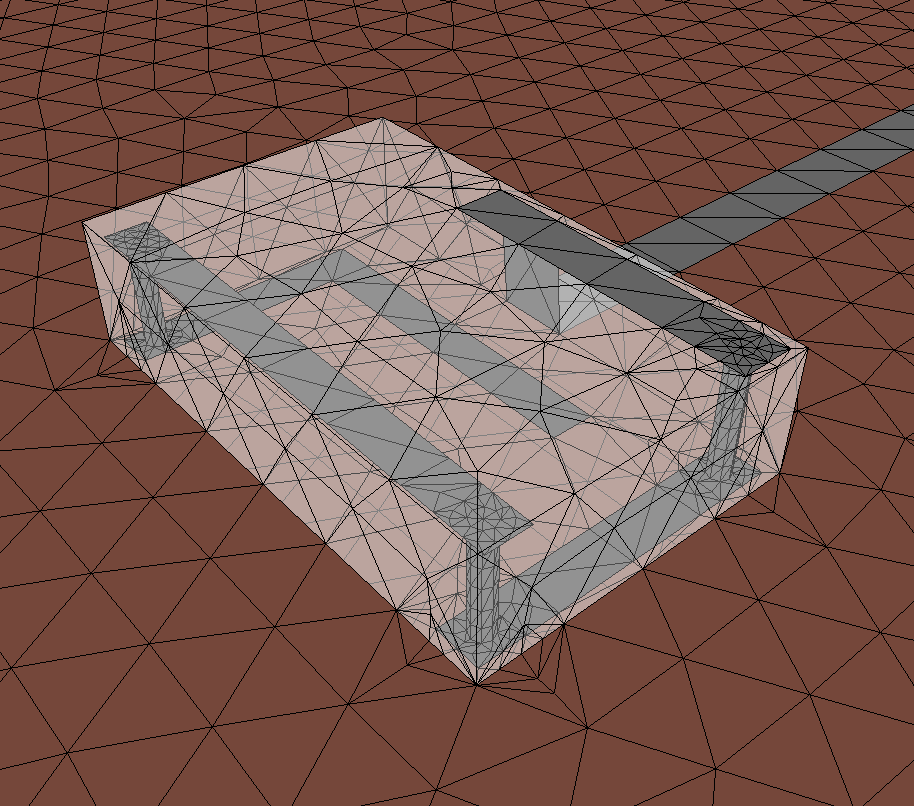
\includegraphics[
		width=0.6\linewidth,
		%trim={0 0 0 0},clip
	]{ltcc}
\end{figure}


Le modèle d'excitation utilisé est le générateur de Thévenin
(section \ref{ssect:the_venin}) avec une impédance réelle de $50$ Ohms.
Le signal du générateur de tension que nous utilisons est une impulsion gaussienne modulée
\eqref{eq:onde_plane_mod} dont les paramètres sont :
\begin{itemize}
	\item $A = 1$ ;
	\item $\freq_0 = 2.4$ GHz ;
	\item $\Delta_\freq = 1$ GHz ;
	\item $a_0 = 0.001$ (ou $0.1$ \%).
	\item $a_A = 0.05$ (ou $5$ \%) ;
\end{itemize}
Avec ces valeurs, la durée du signal est d'environ $6$ ns.
\\


Dans cette
configuration, nous étudions le rayonnement de l’antenne LTCC
placée entre l’avant-bras et le modèle de corps humain complet
(telle une montre connectée),
c’est-à-dire avec $12$ organes pour
lesquels nous disposons des propriétés électriques
représentatives du corps humain \cite{Gabriel1,1996Gabiel,2009Gabriel} :
le cerveau, le cœur, les poumons (2), le foie, la vésicule biliaire, la rate,
le pancréas, les reins (2), une portion du colon, la vessie
ainsi que le squelette avec un haut niveau de détail, du cartilage et la peau.
Le reste du corps est considéré comme étant du muscle.
Les propriétés électriques de ces matériaux sont donnés dans le tableau
\ref{tab:proprietes_mat_corps}.


\begin{figure}[!h]
	\begin{center}
		\caption{
			\label{tab:proprietes_mat_corps}
			Propriétés électromagnétiques des matériaux utilisés
			dans la scène du corps humain complet.
		}
		
		\begin{tabular}{|c|c|c|c|c|}
			\hline
			Matériau & $\EPrm_r$ & $\HPrm_r$ & $\ECnd$ (S/m) & $\HCnd$ \\ \hline\hline
			céramique & $7.8$ & $1$ & $0$ & $0$ \\	\hline
			FR$4$ & $4.4$ & $1$ & $0.01$ & $0$ \\	\hline
			cerveau & $48.34$ & $1$ & $2.02$ & $0$ \\	\hline
			cœur & $58.67$ & $1$ & $3.02$ & $0$ \\	\hline
			poumon & $22$ & $1$ & $0.36$ & $0$ \\	\hline
			foie & $41.82$ & $1$ & $1.9$ & $0$ \\	\hline
			bile & $60$ & $1$ & $2$ & $0$ \\	\hline
			rate & $56.75$ & $1$ & $2.46$ & $0$ \\	\hline
			pancréas & $56.75$ & $1$ & $2.46$ & $0$ \\	\hline
			rein & $56.83$ & $1$ & $2.62$ & $0$ \\	\hline
			colon & $48.5$ & $1$ & $0.93$ & $0$ \\	\hline
			vessie & $20$ & $1$ & $0.7$ & $0$ \\	\hline
			muscle & $50$ & $1$ & $1.33$ & $0$ \\	\hline
			os & $11.41$ & $1$ & $0.43$ & $0$ \\	\hline
			cartilage & $36$ & $1$ & $1.6$ & $0$ \\	\hline
			vide & $1$ & $1$ & $0$ & $0$ \\	\hline
		\end{tabular}
	\end{center}
\end{figure}


Le maillage du corps complet est issu de la numérisation d'un mannequin
anthropomorphique, le modèle PBU-60 produit par la société Kyoto Kagaku.
L'IRCAD de Strasbourg a réalisé des images $3$-d haute résolution à l’aide d’un
scanner CT (pour « \textit{Computerized Tomography} »).
Ensuite, la société Visible Patient a procédé à la segmentation de ces images
en surfaces. Nous avons par la suite
retravaillé les géométries pour les rendre conformes aux
besoins du calcul numérique (figure \ref{img:kyoto}).

\begin{figure}[!h]
	\centering
	\caption{
		\label{img:kyoto}
		Représentation de la géométrie du corps humain complet
		avec ses $12$ organes (le crâne contient un cerveau).
	}
	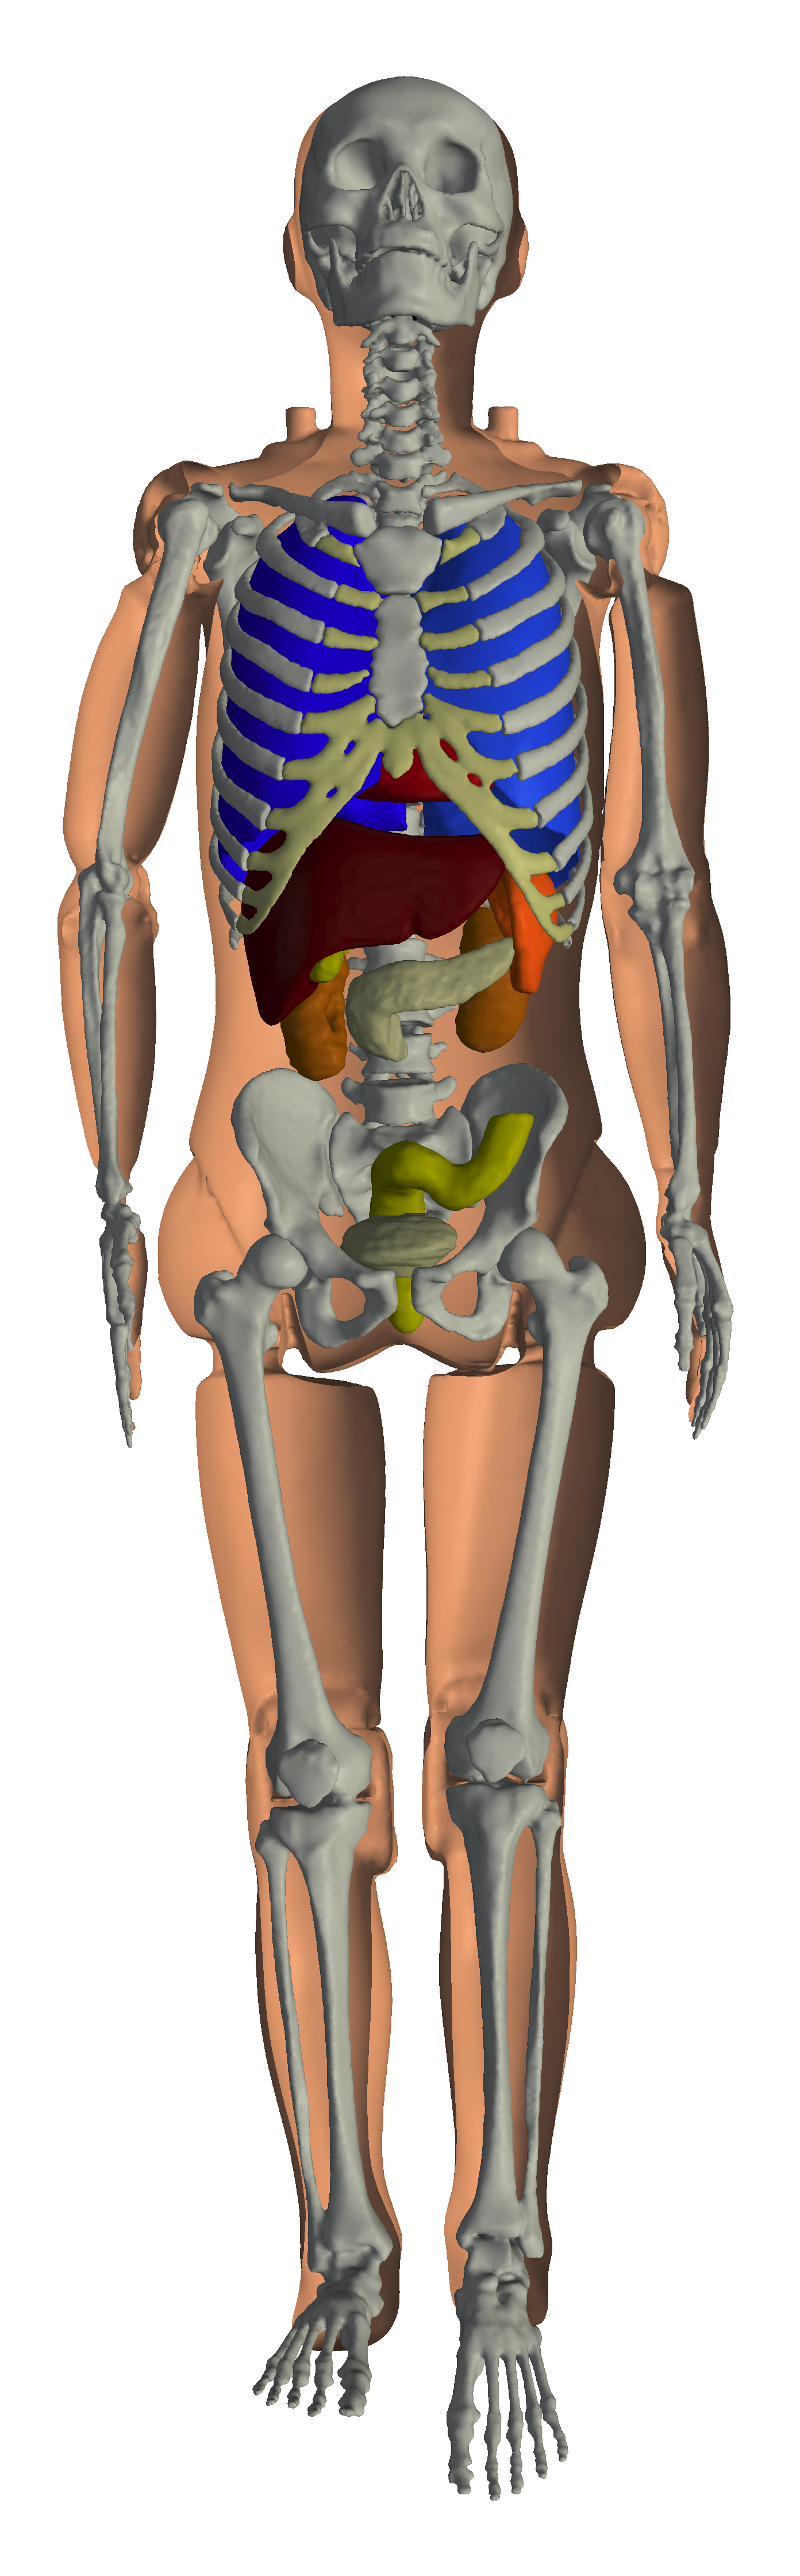
\includegraphics[
	width=0.41\linewidth,
	%trim={0 0 0 0},clip
	]{kyoto}
\end{figure}


Le maillage de la scène simulée est composé de
$5840122$ tétraèdres, soit $23360488$ hexaèdres après
découpage (figure \ref{img:tetra_hexa}) auxquels sont ajoutés
$47340$ mailles de PML (section \ref{ssect:PML}) aux limites du
domaine de calcul.
Cette simulation occupe $40$ Go de
mémoire GPU à l’ordre $\Deg = 1$ (adaptatif), $100$ Go à l’ordre $\Deg = 2$ et
$200$ Go à l’ordre $\Deg = 3$.

Le facteur d'échelle entre la plus petite ($5.076 \cdot 10^{-5}$ m)
et la plus grande ($5.781 \cdot 10^{-2}$ m) arête
de tétraèdre du maillage est de $1139$. Ce facteur passe à $863$
si nous considérons la plus petite arête de chaque tétraèdre.
Après le découpage en hexaèdres, nous obtenons un facteur
d'échelle entre la plus petite ($7.006 \cdot 10^{-6}$ m)
et la plus grande ($3.538 \cdot 10^{-2}$ m) arête
du maillage de $5050$ (hors PML).
Ce facteur passe à $1373$
si nous considérons la plus petite arête de chaque hexaèdre (toujours hors PML).
Ces valeurs témoignent de la forte déformation des hexaèdres
issus du découpage de tétraèdres.
\\


La simulation a nécessité environ
$2091$ heures machine dont $2072$ heures de calcul GPU
pour réaliser $10$ ns de temps physique
à l’aide de la technique de l’ordre adaptatif sur 
la machine de calcul possédée par AxesSim.
Le choix de l'ordre adaptatif a été fait car
cette machine est composée de $8$ GPU NVidia GeForce GTX 1080 Ti
possédant chacun une mémoire de $11$ Go, soit un total de $88$ Go.
Chaque GPU a donc traité environ $5$ Go de données
pendant $10.79$ jours (homme) de calcul pour
une durée totale de simulation de $10.89$ jours en comptant
les $2.34$ heures de pré- et post-traitement et récupération des
données en sortie.


Les données en sortie, principalement sous forme de plans de coupe,
représentent une taille mémoire de $55$ Go.
Un aperçu des résultats sous forme de plan de coupe
est présenté dans la figure \ref{img:kyoto_cutplane}.
Les autres plans de coupe, un par nanoseconde écoulée,
sont présentés en annexe \ref{annexe:kyoto}.

\begin{figure}[!h]
	\centering
	\caption{
		\label{img:kyoto_cutplane}
		Résultats de la simulation sur corps humain complet
		en plan de coupe $(\x_1 O \x_3)$
		en $\x_2 = -0.1255$ m (antenne)
		aux temps $t=2$ ns (à gauche) et $t=4$ ns (à droite).
	}
	\subfloat{
		\label{img:kyoto_cutplane_2ns}
		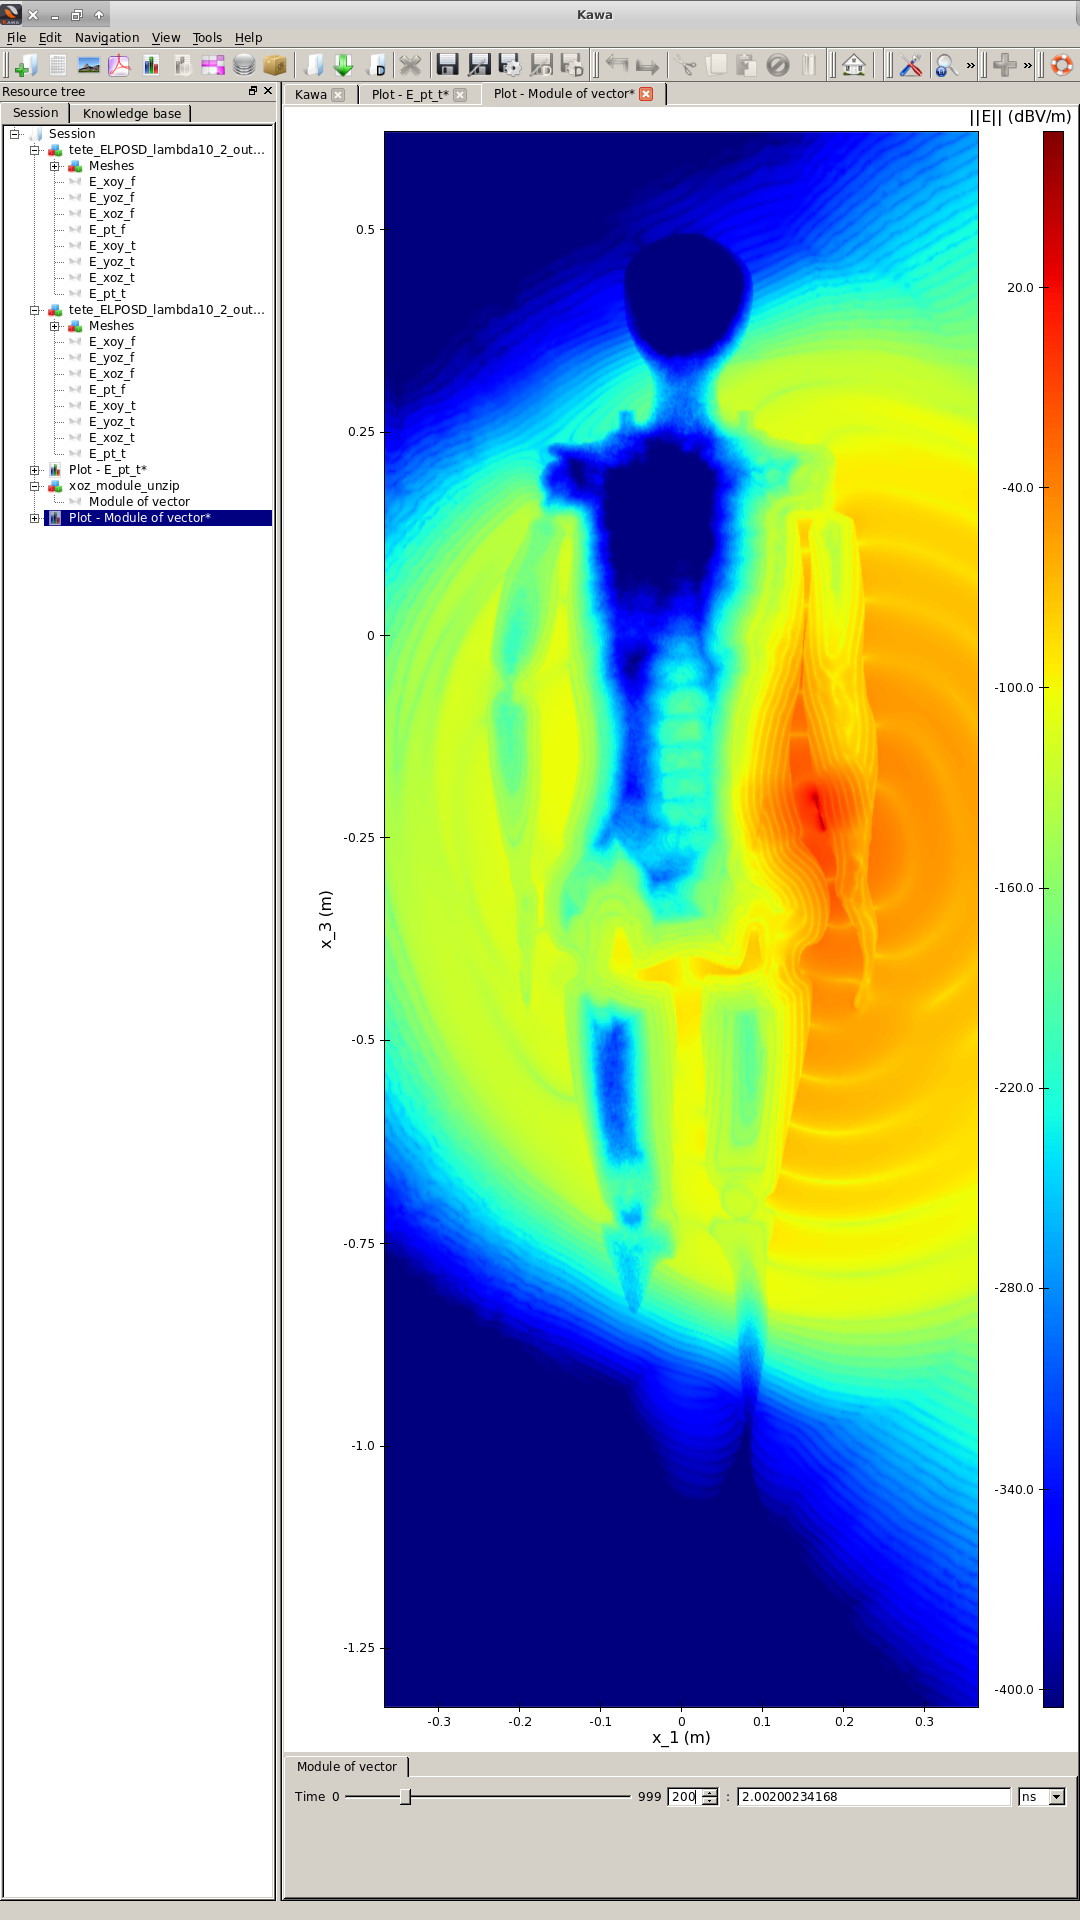
\includegraphics[
		width=0.45\linewidth,
		trim={317 170 8 108},clip
		]{kyoto_2ns}
	}
	\hfill
	\subfloat{
		\label{img:kyoto_cutplane_4ns}
		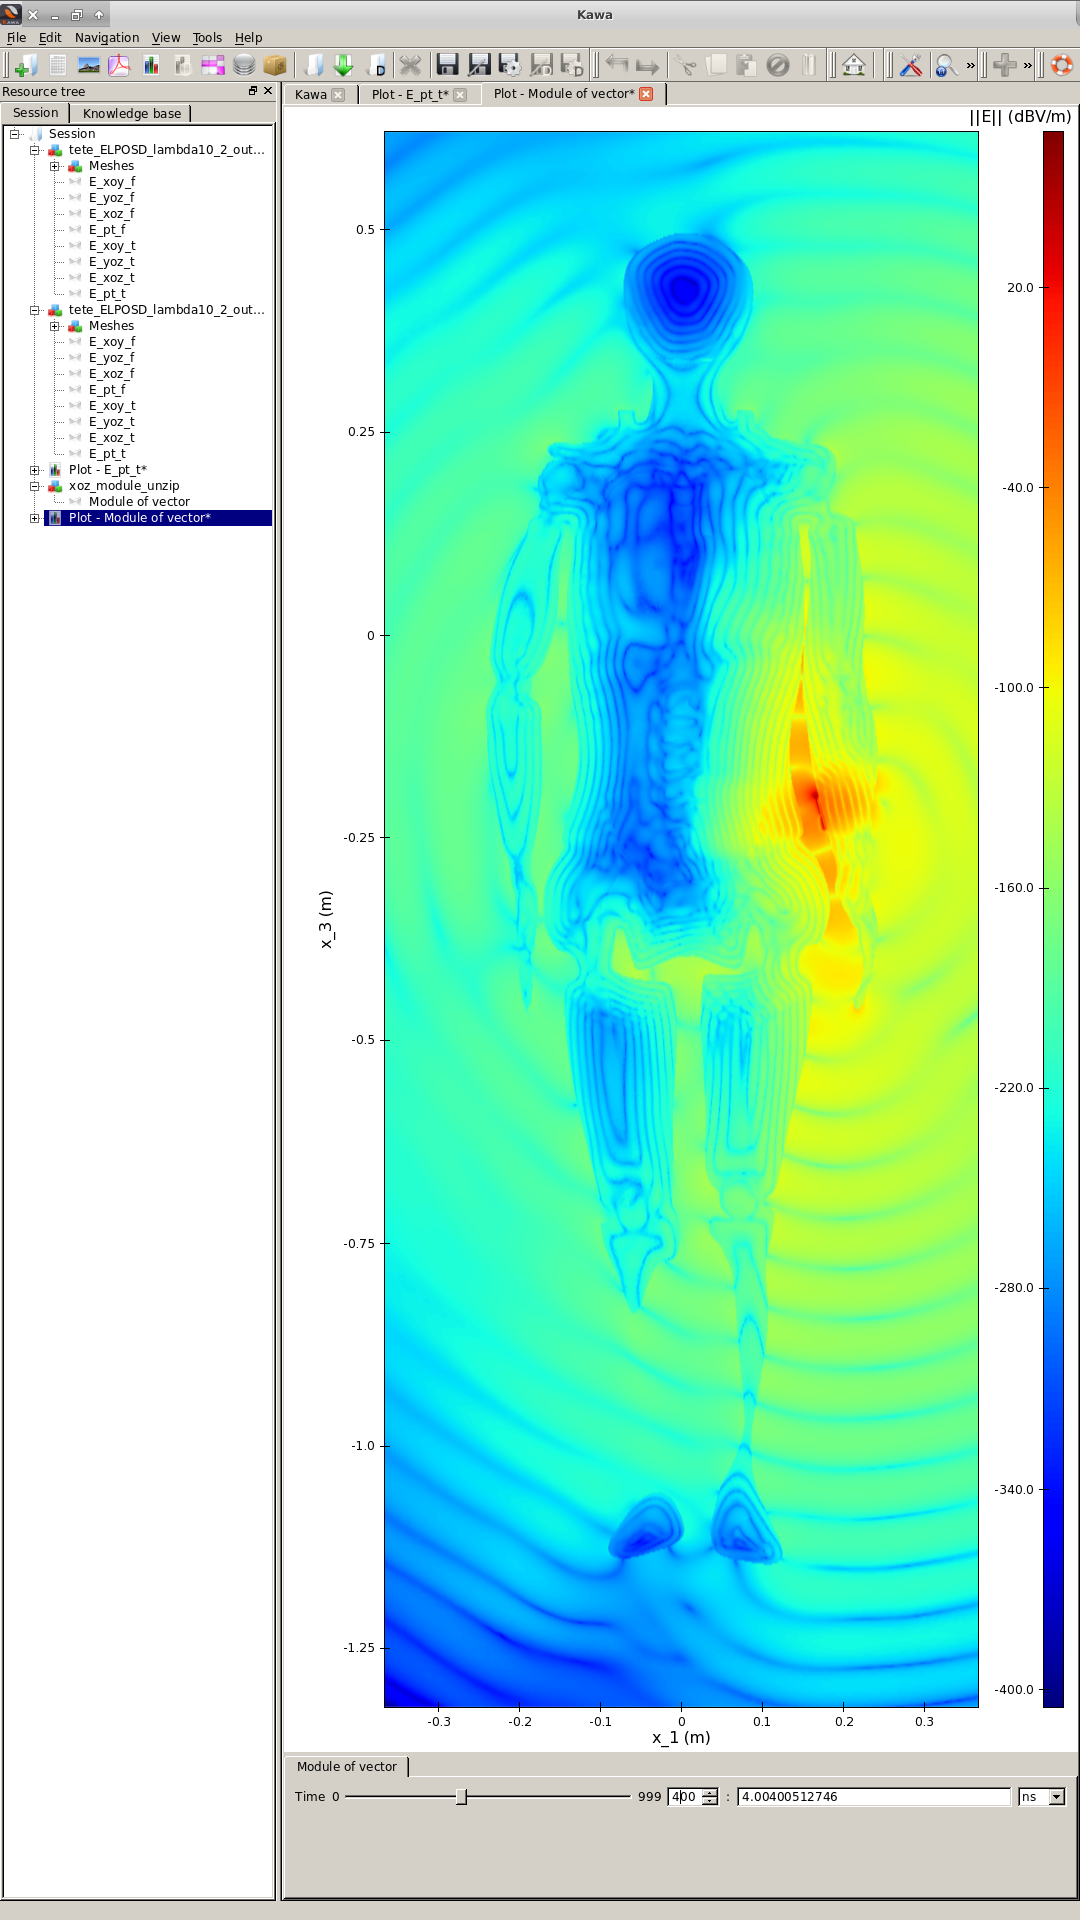
\includegraphics[
		width=0.45\linewidth,
		trim={317 170 8 108},clip
		]{kyoto_4ns}
	}
\end{figure}

Nous pouvons constater la compression de la longueur d'onde
dans les matériaux de forte permittivité et leur absorption
par les tissus présentant une conductivité électrique non nulle.
Les ondes étant plus rapides dans le vide, elles pénètrent
dans le corps du côté droit (opposé à l'antenne) avant l'arrivée des
ondes qui le traversent de part en part dans le sens gauche-droite.
\\


Des tests de scalabilité du solveur ont été effectués
sur cette simulation jusqu'à $256$ GPU pour les ordres
d’interpolation $1$ à $3$. Ces résultats sont présentés dans 
la section \ref{ssect:pizdaint}.
\\



\section{Scalabilité MPI}
\label{sect:scalabilite}


L'implémentation MPI du solveur GD que nous avons présenté dans la
section \ref{ssect:parallelisation_mpi} nécessite de partitionner
le maillage de la scène simulée dans le but d'affecter
une partie à chaque périphérique de calcul.
Ce partitionnement génère des interfaces supplémentaires qui
augmentent le coût de calcul de la simulation.
Ce surcoût diminue l'efficacité du solveur qui doit être étudiée
dans le but de valider l'implémentation MPI.
Nous étudions l'efficacité MPI (ou scalabilité, de l'anglais
« \textit{scaling} ») dans ce chapitre.

Pour cela, outre la machine de calcul possédée par la société
AxesSim, nous avons bénéficié d'heures de calcul sur le Mésocentre
de l'université de Strasbourg et sur le supercalculateur Suisse dénommé PizDaint,
$3^\textrm{ème}$ au TOP500 \cite{Strohmaier:2006:TS:1188455.1188474} jusqu'en juin 2018
avec plus de $25 \; \mathrm{PFlop} \cdot \mathrm{s}^{-1}$, et passé $6^\textrm{ème}$ depuis.
Les heures de calcul sur PizDaint ont été obtenues grâce à l'appel
à projet SHAPE (\textit{SME HPC Adoption Programme in 
Europe}) lancé par PRACE (\textit{Partnership for Advanced Computing in Europe}).
\\



\subsection{Théorie de la scalabilité}
\label{ssect:theorie_scalabilite}

Deux types de scalabilité peuvent être évalués : les scalabilités
faible et forte.

L'évaluation de la \textbf{scalabilité faible}
consiste à traiter un problème de taille proportionnelle
au nombre de périphériques de calcul investis. Pour ce type de scalabilité,
le temps de calcul idéal est constant quelque soit le nombre
de périphériques de calcul.
En pratique, le temps de calcul augmente généralement avec le nombre de
périphériques investis.
Ainsi, le temps de simulation mesuré est de la forme :
\begin{align}
T_\mathrm{s}^k(k \Mesh) = T_\mathrm{s}^1(\Mesh) + P_k^f(\Mesh) ,
\end{align}
où $T_\mathrm{s}^k$ représente le temps de simulation sur $k$
périphériques, $k \Mesh$ représente un maillage dont le nombre
de mailles est $k$ fois plus important que le maillage $\Mesh$ et
avec $(P_k^f)_k$ une suite généralement croissante représentant
la perte d'efficacité sur $k$ périphériques. 
Les valeurs de cette suite dépendent du problème initial.


L'évaluation de la \textbf{scalabilité forte}
consiste à traiter un problème de taille fixe
sur un nombre croissant de périphériques de calcul.
Pour ce type de scalabilité,
le temps de calcul idéal est divisé par le nombre
de périphériques de calcul investis.
Cependant, en pratique, le temps de calcul effectif
est là aussi généralement plus long que le temps idéal.
Ainsi, le temps de simulation mesuré dans ce cas est de la forme :
\begin{align}
T_\mathrm{s}^k(\Mesh) = \frac{T_\mathrm{s}^1(\Mesh)}{k} + P_k^F(\Mesh) ,
\end{align}
avec $(P_k^F)_k$ une suite généralement croissante représentant
la perte d'efficacité en divisant le problème sur $k$ périphériques. 
Là aussi, les valeurs de cette suite dépendent du problème initial.


L'efficacité en scalabilité faible sur $k$ périphériques est donnée par :
\begin{align}
	E_k^f(\Mesh) = \frac{T_\mathrm{s}^1(\Mesh)}{T_\mathrm{s}^k(k\Mesh)}
	= \frac{1}{1 + \frac{P_k^f(\Mesh)}{T_\mathrm{s}^1(\Mesh)}} \le 1 ,
\end{align}
terme de la suite $(E_k^f)_k$, généralement décroissante et positive.

L'efficacité en scalabilité forte sur $k$ périphériques est donnée par :
\begin{align}
	E_k^F(\Mesh) = \frac{T_\mathrm{s}^1(\Mesh)}{k T_\mathrm{s}^k(\Mesh)}
	= \frac{1}{1 + k \frac{P_k^F(\Mesh)}{T_\mathrm{s}^1(\Mesh)}} \le 1 ,
\end{align}
terme de la suite $(E_k^F)_k$, généralement décroissante et positive.

Dans le cas de notre solveur, ces pertes d'efficacité sont
essentiellement générées
par l'augmentation du nombre d'interfaces MPI.
Nous les mesurons dans la suite sur différentes machines de calcul.
\\


\subsection{Machine de calcul AxesSim}
\label{ssect:graph2}

La machine de calcul possédée par AxesSim est composée d'un
CPU Intel Dual Xeon E5-2650 v4
($24$ cœurs physiques hyperthreadés cadencés à $2.20$ GHz)
et de $8$ GPU NVidia GeForce GTX 1080 Ti, chacun regroupant
$3584$ cœurs CUDA cadencés à $1.582$ GHz et possédant $11$ Go de mémoire.

L'unique nœud de cette machine possède $256$ Go de mémoire vive.
Les processus MPI y sont donc tous hébergés en parallèle
et les transferts mémoire sont des transferts internes
à la mémoire vive du nœud, donc très rapides mais aussi très nombreux.

Nous avons mené des tests de scalabilité faible et forte
jusqu'à $8$ GPU sur cette machine.
Les cas d'application utilisés pour ces tests sont semblables à celui
qui nous a permis de déterminer la convergence du schéma couplé
GD-RK$2$ (section \ref{sect:valid_onde_plane}).
Nous simulons une onde plane dans un cube dont nous paramétrons la
taille et le raffinement selon le besoin. Les tailles des maillages utilisés
sont approximativement les termes d'une suite géométrique de raison $2$.
Nous évaluons ainsi la scalabilité du solveur
pour des tailles de maillage allant de $10$ mille à $16$ millions de mailles.
Les résultats d'efficacité sont présentés dans le tableau \ref{tab:scala_graph2}.


\begin{figure}[!h]
	\begin{center}
		\caption{
			\label{tab:scala_graph2}
			Efficacité du schéma couplé GD-RK$2$ à l'ordre spatial $\Deg = 2$
			sur GPU NVidia GeForce GTX 1080 Ti.
			La correspondance explicite en nombre de mailles et la taille mémoire
			correspondante sont uniquement précisés dans le second tableau.
		}
		
		\subfloat[Scalabilité faible (maillage proportionnel).]{
			\label{tab:scala_graph2_faible}
		\begin{tabular}{|c|c|c|c|c|c|c|}
			\hline
			$1$ GPU &
			\multicolumn{2}{c|}{$2$ GPU} &
			\multicolumn{2}{c|}{$4$ GPU} &
			\multicolumn{2}{c|}{$8$ GPU} \\ \hline
			$\#\Mesh$ &
			$\#2\Mesh$ & $E_2^f$ &
			$\#4\Mesh$ & $E_4^f$ &
			$\#8\Mesh$ & $E_8^f$ \\ \hline\hline
			$22^3$ & $28^3$ & $0.728$ & $35^3$ & $0.620$ & $44^3$ & $0.494$ \\	\hline
			$30^3$ & $38^3$ & $0.769$ & - & - & - & - \\	\hline
			$37^3$ & $47^3$ & $0.807$ & - & - & - & - \\	\hline
			$43^3$ & $55^3$ & $0.743$ & - & - & - & - \\	\hline
			$50^3$ & $63^3$ & $0.885$ & - & - & - & - \\	\hline
			$63^3$ & $80^3$ & $0.891$ & - & - & - & - \\	\hline
			$80^3$ & $101^3$ & $0.965$ & $127^3$ & $0.954$ & $160^3$ & $0.928$ \\	\hline
			$100^3$ & $126^3$ & $0.963$ & $159^3$ & $0.969$ & $200^3$ & $0.944$ \\	\hline
			$126^3$ & $159^3$ & $0.993$ & $201^3$ & $0.989$ & $252^3$ & $0.994$ \\	\hline
		\end{tabular}
		}
		\\
		\subfloat[Scalabilité forte (maillage fixe).]{
			\label{tab:scala_graph2_forte}
		\begin{tabular}{|c|c|c|c|c|}
			\hline
			$\#\Mesh$ & RAM (Go) & $E_2^F$ & $E_4^F$ & $E_8^F$ \\ \hline\hline
			$22^3 \approx 10$k & $0.037$ & $0.347$ & $0.188$ & $0.072$ \\	\hline
			$30^3 \approx 25$k & $0.088$ & $0.671$ & - & - \\	\hline
			$37^3 \approx 50$k & $0.156$ & $0.725$ & - & - \\	\hline
			$43^3 \approx 75$k & $0.236$ & $0.891$ & - & - \\	\hline
			$50^3 \approx 125$k & $0.356$ & $0.689$ & - & - \\	\hline
			$63^3 \approx 250$k & $0.672$ & $0.850$ & - & - \\	\hline
			$80^3 \approx 500$k & $1.302$ & $0.883$ & - & - \\	\hline
			$100^3 \approx 1$M & $2.426$ & $0.923$ & $0.793$ & $0.624$ \\	\hline
			$126^3 \approx 2$M & $4.852$ & $0.962$ & $0.845$ & $0.734$ \\	\hline
		\end{tabular}
		}
	\end{center}
\end{figure}




Nous remarquons que le solveur est très efficace en scalabilité faible ($E_k^f > 0.9$)
pour des tailles de maillage supérieures à $500$k mailles par GPU.
Cette taille de maillage correspond à environ $1.3$ Go de mémoire par GPU
à l'ordre d'interpolation spatiale $\Deg = 2$, soit environ $12$ \% de la mémoire
globale d'un GPU NVidia GeForce GTX 1080 Ti.

Les résultats en scalabilité forte rejoignent ceux de la scalabilité faible :
le solveur est fortement scalable sur $2$ GPU avec un maillage
initial de taille supérieure à $1$ million de mailles, soient $500$k mailles
par GPU.
\\


\subsection{Mésocentre de Strasbourg}
\label{ssect:mesocentre}


Le Mésocentre de Strasbourg met à disposition des étudiants (gratuitement)
et des professionnels de la simulation, des heures de calcul
sur CPU et GPU de différents types.
Nous avons notamment utilisé les GPU NVidia Tesla K$20$m (regroupant
$2496$ cœurs CUDA cadencés à $706$ MHz et possédant $4.6$ Go de mémoire) et les
CPU Intel Xeon de la famille E5-26** (composés de $8$ à $16$ cœurs physiques
cadencés à $2.6$ GHz et possédant $64$ ou $128$ Go de mémoire vive).

Nous avons mené des tests de scalabilité faible et forte
jusqu'à $16$ GPU et $4$ CPU (en OpenCL) sur ce calculateur.
Les cas d'application utilisés pour ces tests sont identiques
à ceux utilisés sur la machine de la société AxesSim (mis à part le dernier
pour des raisons de taille mémoire).
Nous évaluons la scalabilité du solveur
pour des tailles de maillage allant de $10$ mille à $8$ millions de mailles.

Les résultats d'efficacité sur GPU sont présentés dans le tableau \ref{tab:scala_meso}.
Le solveur est très efficace sur ces derniers : l'efficacité en scalabilité faible
est supérieure à $0.9$ à partir d'environ $100$k mailles par GPU
et même supérieure à $1$ à partir de $500$k mailles par GPU !
Ce seuil d'efficacité est à nouveau vérifié en scalabilité forte.
Rappelons que, contrairement à la machine de calcul possédée par AxesSim,
tous les GPU ne sont pas associés au même nœud sur le Mésocentre.
Les transferts MPI sont donc répartis entre les différents nœuds sollicités.


\begin{figure}[!h]
	\begin{center}
		\caption{
			\label{tab:scala_meso}
			Efficacité du schéma couplé GD-RK$2$ à l'ordre spatial $\Deg = 2$
			sur GPU NVidia Tesla K$20$m.
			La correspondance explicite en nombre de mailles et la taille mémoire
			correspondante sont uniquement précisés dans le second tableau.
		}
		
		\subfloat[Scalabilité faible (maillage proportionnel).]{
			\label{tab:scala_meso_faible}
			\begin{tabular}{|c|c|c|c|c|c|c|c|c|}
				\hline
				$1$ GPU &
				\multicolumn{2}{c|}{$2$ GPU} &
				\multicolumn{2}{c|}{$4$ GPU} &
				\multicolumn{2}{c|}{$8$ GPU} &
				\multicolumn{2}{c|}{$16$ GPU} \\ \hline
				$\#\Mesh$ & 
				$\#2\Mesh$ & $E_2^f$ &
				$\#4\Mesh$ & $E_4^f$ &
				$\#8\Mesh$ & $E_8^f$ &
				$\#16\Mesh$ & $E_{16}^f$ \\ \hline\hline
				$22^3$ & $28^3$ & $0.482$ & - & - & - & - & - & - \\	\hline
				$30^3$ & $38^3$ & $0.706$ & - & - & - & - & - & - \\	\hline
				$37^3$ & $47^3$ & $0.861$ & - & - & - & - & - & - \\	\hline
				$43^3$ & $55^3$ & $0.913$ & - & - & - & - & - & - \\	\hline
				$50^3$ & $63^3$ & $0.993$ & $80^3$ & $0.941$ & - & - & - & - \\	\hline
				$63^3$ & $80^3$ & $0.977$ & $101^3$ & $0.940$ & - & - & - & - \\	\hline
				$80^3$ & $101^3$ & $1.004$ & $127^3$ & $1.006$ & $160^3$ & $1.012$ & $202^3$ & $0.950$ \\	\hline
				$100^3$ & $126^3$ & $1.011$ & $159^3$ & $1.015$ & $200^3$ & $1.033$ & - & - \\	\hline
				$122^3$ & $154^3$ & $1.009$ & $194^3$ & $1.022$ & - & - & - & - \\	\hline
			\end{tabular}
		}
		\\
		\subfloat[Scalabilité forte (maillage fixe).]{
			\label{tab:scala_meso_forte}
			\begin{tabular}{|c|c|c|c|c|c|}
				\hline
				$\#\Mesh$ & RAM (Go) & $E_2^F$ & $E_4^F$ & $E_8^F$ & $E_{16}^F$ \\ \hline\hline
				$22^3 \approx 10$k & $0.037$ & $0.323$ & - & - & - \\	\hline
				$30^3 \approx 25$k & $0.088$ & $0.515$ & - & - & - \\	\hline
				$37^3 \approx 50$k & $0.156$ & $0.659$ & - & - & - \\	\hline
				$43^3 \approx 75$k & $0.236$ & $0.761$ & - & - & - \\	\hline
				$50^3 \approx 125$k & $0.356$ & $0.874$ & - & - & - \\	\hline
				$63^3 \approx 250$k & $0.672$ & $0.925$ & $0.689$ & - & - \\	\hline
				$80^3 \approx 500$k & $1.302$ & $0.952$ & $0.854$ & $0.717$ & $0.468$ \\	\hline
				$100^3 \approx 1$M & $2.426$ & $0.961$ & $0.861$ & $0.754$ & $0.597$ \\	\hline
				$122^3 \approx 1.8$M & $4.243$ & $0.966$ & $0.905$ & $0.834$ & $0.638$ \\	\hline
			\end{tabular}
		}
	\end{center}
\end{figure}



Sur CPU, les résultats en scalabilité faible sont inférieurs.
Pour un maillage initial
de $500$k mailles (seuil identifié sur la machine de calcul possédée par AxesSim)
l'efficacité est d'environ $0.8$.
Cette baisse est principalement dûe au fait que le masquage des communications
MPI par l'exécution des kernels OpenCL n'est plus possible. En effet,
lors de l'exécution d'un kernel OpenCL sur CPU, tous les cœurs sont sollicités.
Le kernel et les communications MPI sont donc mis en concurrence et mutuellement ralentis.
Dans les versions récentes d'OpenCL, un CPU peut être subdivisé pour libérer des
cœurs de calcul. Il s'agit là d'une piste pour améliorer l'efficacité sur CPU.

Toujours sur CPU, en scalabilité forte, l'efficacité est généralement supérieure à $0.9$
à partir du seuil de $500$k mailles par périphérique.
Ce résultat pourrait s'expliquer par le fait que la réduction de la taille des kernels
laisse progressivement plus de place aux communications MPI, elles-mêmes
plus courtes, bien que plus nombreuses.
Cela dit, la réduction de la taille des kernels peut aussi induire
l'apparition d'effets de cache.
\\
%\todo{pas certain: peut-être aussi un effet de cache}


\subsection{PizDaint via PRACE}
\label{ssect:pizdaint}

Suite à l'appel à projet SHAPE lancé par PRACE dans le but
de rendre les supercalculateurs européens accessibles aux PME
européennes, la société AxesSim a obtenu $2000$ heures
de calcul sur le supercalculateur PizDaint.
Cette machine est équipée de plus de $5000$ GPU NVidia Tesla P$100$,
équivalents en terme de performance au GPU NVidia GeForce GTX 1080 Ti.

L'objectif était d'utiliser ces heures de calcul pour effectuer des simulations
sur le corps humain complet (avec organes). Cependant, après la première
simulation effectuée sur la machine de calcul possédée par AxesSim, nous
avons constaté que ce quota d'heures était insuffisant pour une unique simulation.
Nous avons donc utilisé ces heures pour effectuer des tests de scalabilité forte
sur la configuration présentée sans la section \ref{ssect:corps_complet}.

Nous sommes arrivés jusqu'à l'utilisation simultanée de $256$ GPU
\cite{prace_whitepaper}, une première pour le solveur \texttt{teta-clac}.
Les résultats sont présentés dans le tableau \ref{tab:scala_pizdaint}.
Les temps de référence qui ont permis de calculer
ces efficacités n'ont pas été obtenus sur un seul GPU mais sur un nombre
croissant de GPU en fonction de l'ordre spatial. En effet,
la taille mémoire nécessaire rend impossible la simulation sur un seul GPU.


\begin{figure}[!h]
	\begin{center}
		\caption{
			\label{tab:scala_pizdaint}
			Efficacité du schéma couplé GD-RK$2$ sur la configuration
			du corps humain complet pour différents ordres d'interpolation
			sur GPU NVidia Tesla P$100$.
		}
		
		\begin{tabular}{|c|c|c|c|}
			\hline
			$\#$GPU & $\Deg = 1$ (*) & $\Deg = 2$ & $\Deg = 3$ \\ \hline\hline
			$4$ & $1$ (**) & - & - \\	\hline
			$8$ & $0.980$ & $1$ (**) & - \\	\hline
			$16$ & $0.955$ & $0.980$ & $1$ (**) \\	\hline
			$32$ & $0.909$ & $0.943$ & $0.970$ \\	\hline
			$64$ & $0.844$ & $0.889$ & $0.919$ \\	\hline
			$128$ & $0.749$ & - & - \\	\hline
			$256$ & $0.612$ & - & - \\	\hline
		\end{tabular}
		\\
		(*) \textit{Simulations en ordre spatial adaptatif (PML à l'ordre 2).}
		\\
		(**) \textit{Simulation prise comme référence pour l'ordre courant.}
	\end{center}
\end{figure}


Nous constatons que la scalabilité du solveur est très
bonne sur ce cas d'application.
L’efficacité du solveur à l’ordre (adaptatif) $1$ sur $256$ GPU
est de $0.612$ par rapport à une exécution sur $4$ GPU,
soit une efficacité de $0.6$ par rapport à $8$ GPU.
Ce qui signifie que le temps GPU
nécessaire à l’exécution sur $256$ GPU est d’environ
$3454$ heures pour réaliser $10$ ns de temps physique
mais avec un temps réel de restitution d’environ $13.5$ heures (homme).


Notons que le coefficient CFL utilisé pour cette simulation est naïvement de
$0.9$ ($\dt = 3.165 \cdot 10^{-15}$ s) et pourrait très certainement être augmenté par la méthode
de la puissance itérée (section \ref{ssect:puissance itérée}).
Ce temps pourra encore être réduit avec l'application du schéma LTS$2$
(section \ref{sect:pas de temps local}), lorsque ce dernier
sera pleinement fonctionnel en MPI.
\\



\section*{Conclusion}


Dans ce dernier chapitre, nous avons présenté des résultats
permettant de valider notre implémentation de solveur GD, autant
par la précision des calculs que par leur vitesse d'exécution.

Dans un premier temps, nous avons présenté des résultats de convergence
et de précision 
sur un cas académique de propagation d'une onde plane dans un cube
pour différents ordres d'interpolation.
L'ordre de convergence théorique du schéma en temps a été vérifié
en pratique et l'erreur globale commise reste négligeable.
Ces résultats ont été obtenus sur maillages structurés et non structurés
et démontrent le bon fonctionnement du solveur ainsi que sa
polyvalence du point de vue géométrique.
Nous avons aussi comparé les caractéristiques des maillages
étudiés, notamment leur nombre de mailles et la taille
des arêtes afin de dégager un ordre de grandeur du malus
dont bénéficient les maillages en tétraèdres.


Nous avons ensuite comparé notre solveur GD à un solveur implémentant
la méthode des différences finies sur un cas d'application
mettant en scène une antenne dipolaire à proximité de l'oreille d'une tête
humaine simplifiée.
Ce cas d'application présentant peu de formes rectilignes
et une très petite source d'excitation
avantage notre solveur GD en temps de calcul par le faible nombre
de mailles non structurées requises. La grande quantité
d'optimisations est cependant la principale raison
des hautes performances produites par le solveur GD comme en témoignent
les résultats en temps de calcul.
Parmi ces optimisations, la méthode à pas de temps local
présentée dans le chapitre \ref{chap:pas de temps local}
qui permettrait d'obtenir des accélération encore plus importantes
sur un cas tel que celui du corps humain complet.


Nous avons enfin présenté les résultats d'une simulation exécuté
sur le modèle de corps humain complet dans le cadre du projet HOROCH.
Le rayonnement d'une antenne de type Bluetooth placée telle
une montre connectée à proximité du bras a été simulé sur $10$ ns de
temps physique en parallèle sur 8 GPU NVidia de dernière génération.
Rappelons qu'il s'agit de la plus grande simulation réalisée par le solveur
à ce jour. Celle-ci a aussi servi à effectuer des tests d'efficacité allant
jusqu'à 256 GPU ce qui nous a permis de pleinement valider son implémentation MPI.
L'implémentation MPI de la méthode à pas de temps local
n'a pas encore été finalisée mais devrait permettre de significativement
réduire le temps de calcul.





\cleardoublepage
\chapter*{Conclusion}
\addcontentsline{toc}{chapter}{Conclusion}


Dans cette thèse, nous avons commencé par rappeler
les équations de Maxwell et montré qu’elles constituent un système
hyperbolique dit de Friedrichs (chapitre~\ref{chap:generalites}).
Ce système a ensuite été présenté sous sa forme Galerkin Discontinue (GD)
qui fait intervenir un flux numérique que nous avons choisi décentré
afin d'améliorer la stabilité du schéma.
Nous avons également caractérisé les
conditions limites permettant d’assurer cette stabilité.
La formulation GD a ensuite été présentée sous sa forme semi-discrète
dont la solution converge vers celle du problème continu (annexe~\ref{annexe:demo_cv}).
\\

Nous avons ensuite présenté plusieurs modèles de simulation
qui permettent de faciliter la génération de la scène simulée
et de réduire le temps de calcul (chapitre~\ref{chap:modeles}).

Nous avons commencé par décrire des modèles de conditions de bord
respectant la condition d'existence de la solution, notamment
la condition de Silver-Müller ainsi que les couches absorbantes PML
très utilisées dans les applications industrielles.
Grâce à ces modèles, le domaine de calcul peut être borné
au plus près de la zone d'intérêt tout en limitant les
réflexions qui viendraient polluer le domaine de calcul.

Nous avons aussi donné un ensemble de modèles permettant de simuler
les plaques minces de matériaux. Ces modèles permettent de remplacer
les volumes fins par des surfaces, sont complémentaires sur une
large bande de fréquences, et réduisent les temps de simulation
tout en facilitant la phase de maillage.
\\


L'implémentation de la méthode GD que nous avons présentée
(chapitre~\ref{chap:implementation}) utilise un espace
d'approximation hexaédrique discrétisé par les points de
Gauss-Legendre et muni des produits tensoriels des polynômes de Lagrange
qui s'appuient sur ces points.
Les propriétés de cet espace d'approximation
simplifient les formules de quadrature par l'annulation
du gradient des fonctions de base en de nombreux points d'interpolation.
Ces simplifications n'apparaissent pas dans les mailles tétraédriques.

Nous pourions aussi utiliser les points d'interpolation de Gauss-Lobatto
qui produiraient d'importantes simplifications au niveau du terme
de flux. Dans ce cas les points de bord sont placés sur les interfaces
et l'extrapolation/application des champs sur le volume n'est plus
nécessaire. Ils permettent aussi d'appliquer un schéma de type
« \textit{split form} » qui conserve mieux l'empreinte fréquentielle
du signal.
Ces points feront l'objet de futurs travaux sur le solveur.

Nous avons aussi présenté les schémas de type Runge-Kutta
qui nous permettent d'intégrer temporellement la solution
afin d'avancer cette dernière jusqu'au temps final souhaité.
Néanmoins, la stabilité de la méthode RK$2$ et directement
liée à la taille et la forme des mailles, ce qui complique
son utilisation dans les applications en tétraèdres découpés.
Nous avons donc présenté $2$ conditions de stabilité de type CFL
ainsi que $2$ diagnostics de stabilité : le calcul des valeurs propres
du système et la puissance itérée.
Ce second diagnostic permet de déterminer avec précision le coefficient
CFL de stabilité. Une implémentation OpenCL du calcul de la norme
utilisée dans cette méthode
nous permettra de déterminer ce coefficient rapidement et systématiquement
en procédant à une dichotomie.
\\


Cette implémentation de la méthode GD a été programmée
à destination des GPU en utilisant la bibliothèque OpenCL
(chapitre~\ref{chap:parallelisations_et_optimisations}).
La parallélisation sur plusieurs GPU est asurée via
une implémentation du standard MPI.
Le partitionnement du maillage est automatiquement généré
à l'exécution afin de répartir la charge de calcul
de façon équilibrée entre les accélérateurs.
Toutes ces capacités permettent au solveur \texttt{teta-clac}
de facilement résoudre des problèmes de grande taille sur un nombre
quelconque de GPU.

Nous avons aussi décrit les adaptations qui ont été menées dans le
but d'optimiser les kernels de calcul OpenCL à destination des CPU.
Les performances ont été nettement améliorées sur ce type
de périphériques mais restent dépendantes des caractéristiques
du périphérique en lui-même.

Enfin, nous avons présenté la méthode de l'ordre d'interpolation
spatiale adaptatif qui permet de corriger automatiquement la discrétisation
dans les zones sur- ou sous-maillées.
Cette méthode nous permet de mailler avec précisions (par de petites mailles)
des géométries présentant un haut niveau de détail :
l'ordre d'interpolation y sera automatiquement abaissé pour réduire le
temps de calcul.
Nous avons néanmoins constaté qu'un ordre d'interpolation trop faible
risque de dénaturer le signal. Il est donc préférable
de projeter l'utilisation d'un ordre d'interpolation élevé
afin de conserver un ordre abaissé supérieur à $1$.
\\



Nous avons ensuite énoncé
une variante locale de la méthode GD qui
permet d'alléger les calculs de flux et de découpler l'avancée en
temps des mailles (chapitre~\ref{chap:pas de temps local}).
Cet opérateur local nous a permis de décrire deux schémas temporels.
Premièrement, le schéma LRK$2$ qui est une implémentation à prédiction locale
du schéma RK$2$. Ce schéma utilise
un pas de temps homogène sur tout le maillage.
Il a expérimentalement été démontré convergeant et stable.

Nous avons aussi présenté le schéma LTS$2$ pour lequel le pas de
temps est local à chaque maille.
Les accélérations obtenues à l'aide de cette méthode sont
très proches de l'accélération théorique en dimension $1$.
Nous constatons aussi une accélération des calculs
en dimension $3$, mais plus éloignée des valeurs théoriques.
Ce schéma n'est adapté qu'aux géométries composées de mailles de tailles très hétérogènes. Dans le cas d'un facteur d'échelle entre la plus petite
et la plus grande maille de l'ordre de $100$, le surcoût engendré par
la multiplication des interfaces est tout juste amorti et un faible
gain de temps est constaté ($\approx 35$ \% à l'ordre $\Deg = 1$ et
$\approx 27$ \% à l'ordre $\Deg = 2$). Cette méthode
devrait cependant montrer de bien meilleures accélérations
sur un cas tel que celui du corps humain complet
qui présente un facteur d'échelle $10$ fois plus important.
\\



Pour répondre à la problématique des architectures hybrides
et devant le complexité de certains graphes des tâches,
nous avons décrit 
l'utilisation de la bibliothèque StarPU pour l'exécution
et l'ordonnancement des tâches de calcul du solveur GD \texttt{schnaps}
(chapitre~\ref{chap:runtimes}).
Les résultats sur CPU multi-cœurs se sont avérés excellents :
une efficacité presque optimale quelque soit le nombre de cœurs
sollicités et pour diverses tailles (divers raffinements) du problème étudié.

Les résultats en configuration hybride sont eux aussi
de bonne qualité.
Nous avons constaté que l'ajout des cœurs CPU au GPU
a permis d'améliorer les performances du GPU seul.
Dans le cas des plus petites tailles de problème,
l'accélération constatée est au-delà de
l'accélération théorique donnée par les temps sur CPU seul et GPU seul.
\\



Nous sommes ensuite revenus sur le solveur \texttt{teta-clac}
et avons présenté des résultats
permettant de valider notre implémentation de solveur GD, autant
par la précision des calculs que par leur vitesse d'exécution
(chapitre~\ref{chap:validation}).

Dans un premier temps, nous avons présenté des résultats de convergence
et de précision
sur un cas académique de propagation d'une onde plane dans un cube
pour différents ordres d'interpolation.
L'ordre de convergence théorique du schéma en temps a été vérifié
en pratique et l'erreur globale commise reste négligeable.
Ces résultats ont été obtenus sur maillages structurés et non structurés
et démontrent le bon fonctionnement du solveur ainsi que sa
polyvalence du point de vue géométrique.

Nous avons ensuite comparé notre solveur GD à un solveur implémentant
la méthode des différences finies (FD) sur un cas d'application
mettant en scène une antenne dipolaire à proximité de l'oreille d'une tête
humaine simplifiée.
La grande quantité d'optimisations ont permis à notre solveur GD
de produire de hautes performances et de meilleurs temps de calcul
que le solveur FD.
\\

Nous avons enfin présenté les résultats d'une simulation exécutée
sur le modèle de corps humain complet dans le cadre du projet HOROCH.
Une simulation de $10$ ns de temps physique en parallèle sur
$8$ GPU NVidia de dernière génération.
Cette simulation démontre la capacité du solveur \texttt{teta-clac}
à traiter des problèmes de rayonnement
électromagnétique d'objets connectés placés à proximité
(ou à l'intérieur) du corps humain.

Précisons que le temps de simulation sur corps humain complet
donné à $11$ jours est issu d'un premier essai.
L'utilisation d'un coefficient CFL plus adaptée devrait permettre
de réduire ce temps de restitution (facteur d'accélération proche de $5$ dans le
cas de la tête humaine simplifiée à l'ordre d'interpolation $1$).
La finalisation de l'implémentation MPI du schéma LTS$2$ devrait
aussi permettre de constater un important gain de temps compte tenu
du facteur d'échelle proche de $1000$ entre la plus petite et
la plus grande maille.

Cette simulation a aussi permis d'effectuer des tests de
scalabilité MPI allant jusqu'à 256 GPU.
Nous avons alors évalué qu'elle pouvait être réalisée
en moins d'un jour sur $256$ GPU.
Ces tests témoignent du fait que le temps de calcul
d'une simulation peut être compressé en investissant plus
de ressources de calcul et ainsi passer de plus de $10$ jours
à seulement quelques heures d'attente avant la restitution des données.
C'est l'amélioration constante du solveur GD \texttt{teta-clac}
qui nous a permis d'obtenir ces résultats encore hypothétiques
il y a $3$ ans.
\\





\cleardoublepage
\appendix
\chapter{Existence de la solution du problème d'évolution}
\label{annexe:demo_existence}


\section{Théorie des opérateurs linéaires}
\label{sect:theorie_operateurs_lineaires}

Le théorème de Hille-Yosida est un théorème abstrait de la théorie des
opérateurs linéaires qui permet de démontrer l'existence et l'unicité
de la solution d'un problème d'évolution. Nous donnons les notions
minimales pour comprendre l'énoncé de ce théorème.
Pour plus de détails, nous renvoyons au livre de Brézis
\cite{brezis1983analyse}.
\\

Nous considérons un espace de Hilbert $H$
muni du produit scalaire $\left\langle \cdot , \cdot \right\rangle$.
En général, $\A$ désignera un opérateur non-borné de $H$
à domaine dense, c'est à dire une application linéaire d'un sous-espace vectoriel $D(\A)$ de $H$ à valeurs dans $H$.
Le sous-espace vectoriel $D(\A)$ est appelé domaine de $\A$.
Si $H$ est un Hilbert de dimension infinie, $D(\A)$
n'est généralement pas fermé. Nous supposons que le domaine de $\A$
est dense, c'est à dire que $\Adh{D(\A)} = H$ pour la topologie forte de $H$.
La topologie forte est la topologie associée à la norme du produit scalaire
de $H$. Le graphe de $\A$, noté $G(\A)$ est l'ensemble :
\begin{align}
	G(\A) = \left\{ (\U,\A \U) : \U \in D(\A) \right\} \subset H^2 .
\end{align}
En général, $\Adh{G(\A)}$
n'est pas le graphe d'un opérateur univoque, c'est à dire que
$(\U,\Vec{f}) \in \Adh{G(\A)}$ et $(\U,\Vec{g}) \in \Adh{G(\A)}$
n'implique pas forcément $\Vec{f} = \Vec{g}$.
Si $\Adh{G(\A)}$ est le graphe d'un opérateur univoque, nous dirons que $\A$
est un opérateur non-borné fermable. Nous appellerons fermeture de $\A$
et nous noterons $\Adh{\A}$ l'opérateur tel que $G(\Adh{\A}) = \Adh{G(\A)}$.

\begin{definition}
	Soit $H$ un espace de Hilbert de produit scalaire
	$\left\langle \cdot , \cdot\right\rangle$.
	Soit $\A$ un opérateur linéaire de $D(\A)$, sous-espace vectoriel de $H$,
	dans $H$. $\A$ est dit \textbf{monotone} si :
	\begin{align}
		\forall \U \in D(\A), \left\langle \A \U , \U \right\rangle \ge 0 .
	\end{align}
	L'opérateur $\A$ est dit \textbf{maximal monotone} si de plus
	$\Mat{I} + \A$ est surjectif de $D(\A)$ sur $H$.
\end{definition}

Considérons le problème d'évolution abstrait d'inconnue
$\U(t) \in D(\A)$ :
\begin{subequations} \label{eq:pb_abstrait}
	\begin{align}
		\Ptl{t} \U + \A \U &= 0 , \\
		\U(0) &= \U_{0} \in D(\A) .
	\end{align}
\end{subequations}
Le théorème de Hille-Yosida donne une condition pour que ce problème soit
bien posé. Dans le cas qui nous intéresse, l'opérateur $\A$
sera formellement l'opérateur aux dérivées partielles en espace
$\Aidi$ et son domaine $D(\A)$ sera l'ensemble des $\W$
qui satisfont les conditions aux limites.

\begin{theorem}[Hille-Yosida]
	Si $\A$ est maximal monotone, alors le problème \eqref{eq:pb_abstrait}
	admet une unique solution $\U$ dans
	$\mathcal{C}^{1}(\PbTps,H) \cap \mathcal{C}(\PbTps,D(\A))$
	et pour tout $t$ :
	\begin{align}
		\Norm{\U(t)} \le \Norm{\U_0}, \;
		\Norm{\Ptl{t} \U(t)} =
		\Norm{\A \U(t)} \le \Norm{\A \U_0} .
	\end{align}
\end{theorem}

\begin{remark}
	$D(\A)$ est muni de la norme dite du graphe :
	\begin{align}
		\Norm{\U}_{D(\A)} = \Norm{\U}_{H} + \Norm{\A \U}_{H} .
	\end{align}
\end{remark}

\begin{remark}
	L'application qui à $\U_0$ associe $\U(t)$
	peut donc être prolongée par densité en un semi-groupe
	de contrations de $H$ dans $H$.
	Il est donc possible de définir des solutions du problème
	d'évolution lorsque $\U_0 \in H$.
\end{remark}

Nous allons maintenant introduire quelques outils qui permettront de
démontrer la surjectivité de $\Mat{I} + \A$. Les démonstrations seront basées
sur des techniques d'intégration par parties et de passage à l'adjoint.

\begin{definition}
	Soit $\A$ un opérateur linéaire de $H$ dans $H$ de domaine $D(\A)$ dense.
	$\A^{\#}$ est un \textbf{adjoint formel} de $\A$ si $\A^{\#}$
	est à domaine dense et :
	\begin{align}
		\forall \U \in D(\A), \forall \V \in D(\A^{\#}), \;
		\left\langle \A \U , \V \right\rangle
		= \left\langle \U , \A^{\#} \V \right\rangle .
	\end{align}
\end{definition}

\begin{proposition}
	Si $\A$, un opérateur linéaire de $H$, admet un adjoint formel $\A^{\#}$,
	alors $\A$ est fermable, c'est à dire que la fermeture du graphe de $\A$
	dans $H^2$, $\Adh{G(\A)}$, définit un opérateur univoque.
\end{proposition}

%\tikzset{external/export=false}
%\todo{A vérifier}
%\tikzset{external/export=true}
\begin{proof}
	Soit $(\U_n)_{n \in \EnsN}$ une suite définie sur $D(\A)$
	telle que $\U_n \rightarrow \U$.
	Soient $(\Vec{f}_n)_{n \in \EnsN}$ et $(\Vec{g}_n)_{n \in \EnsN}$
	des suites définies telles que, pour tout $n$ nous ayons
	$(\U_n,\Vec{f}_n) , (\U_n,\Vec{g}_n) \in G(\A)$ et,
	$\Vec{f}_n \rightarrow \Vec{f}$ et $\Vec{g}_n \rightarrow \Vec{g}$.
	Ainsi, $(\U,\Vec{f})$  et $(\U,\Vec{g})$ appartiennent à $\Adh{G(\A)}$.
	Puisque $\A$ admet un adjoint formel $\A^{\#}$, pour tout
	$\V \in \A^{\#}$ et tout $n$, nous avons :
	\begin{align}
		\left\langle \Vec{f}_n , \V \right\rangle =
		\left\langle \Vec{g}_n , \V \right\rangle =
		\left\langle \U_n , \A^{\#} \V \right\rangle .
	\end{align}
	S'ensuit, par linéarité à gauche du produit scalaire :
	\begin{align}
		\left\langle \Vec{f}_n , \V \right\rangle -
		\left\langle \Vec{g}_n , \V \right\rangle =
		\left\langle \Vec{f}_n - \Vec{g}_n , \V \right\rangle = 0 ,
	\end{align}
	et donc $\Vec{f}_n = \Vec{g}_n$.
	En passant à la limite nous obtenons le résultat souhaité.
\end{proof}

\begin{definition}
	Soit $\A$ un opérateur de $H$ dans $H$ à domaine dense.
	L'\textbf{adjoint} (non formel) de $\A$, noté $\A^\star$,
	est un opérateur de $H$ dans $H$
	défini tel que :
	\begin{align}
		D(\A^\star) = \left\{
			v \in H : \exists C \ge 0 : \forall \U \in D(\A),
			\Abs{\left\langle \A \U , \V \right\rangle}
			\le C \Norm{\U}
		\right\} .
	\end{align}
	En d'autres termes, $D(\A^\star)$ est l'ensemble des $\V \in H$
	tel que la forme linéaire
	$\varphi : \U \mapsto \left\langle \A \U, \V \right\rangle$
	est continue sur $D(\A)$ pour la norme de $H$.
	\\
	De plus, si $\V \in D(\A^\star)$, alors $\varphi$
	se prolonge (par densité de $D(\A)$ dans $H$) en une forme linéaire
	continue sur $H$, c'est à dire un élément de l'espace dual de $H$.
	Comme $H$ est un espace de Hilbert, par le théorème de représentation
	de Riesz, il existe un unique $\Vec{f} \in H$ tel que
	$\left\langle \A \U , \V \right\rangle =
	\left\langle \Vec{f} , \U \right\rangle$.
	Alors par définition $\Vec{f} = \A^\star \V$.
\end{definition}

\begin{remark}
	En général, $\A^\star \neq \A^{\#}$. Cependant,
	pour tout adjoint formel $\A^{\#}$, $G(\A^{\#}) \subset G(\A^\star)$
	et ainsi $D(\A^{\#}) \subset D(\A^\star)$.
\end{remark}

\begin{definition}
	Soit $\A$ un opérateur fermable. Soit $\U$ un élément de $H$.
	$\U$ est \textbf{solution forte} de $\A \U = \Vec{f}$ si
	$\Adh{\A} \U = \Vec{f}$.
\end{definition}

Une solution forte $\U$ de $\A \U = \Vec{f}$ est telle que
$(\U,\Vec{f}) \in \Adh{G(\A)} = G(\Adh{\A})$.
En d'autres termes, $\U$ est solution forte de $\A \U = \Vec{f}$
si, et seulement si, il existe une suite
$(\U_n)_{n \in \EnsN}$ d'éléments de $D(\A)$
telle que $\U_n \rightarrow \U$ et $\A \U_n \rightarrow \Vec{f}$.

\begin{definition}
	Soit $\U$ un élément de $H$.
	$\U$ est \textbf{solution faible} de $\A \U = \Vec{f}$
	si $\A$ admet un adjoint formel $\A^{\#}$
	et :
	\begin{align}
		\forall \V \in D(\A^{\#}),
		\left\langle \Vec{f} , \V \right\rangle =
		\left\langle \U , \A^{\#} \V \right\rangle .
	\end{align}
\end{definition}

\begin{proposition}
	Si $\A$ admet un adjoint formel, alors toute solution forte
	de $\A \U = \Vec{f}$ est aussi solution faible.
\end{proposition}

%\tikzset{external/export=false}
%\todo{A vérifier}
%\tikzset{external/export=true}
\begin{proof}
	Soit $(\U_n)_{n \in \EnsN}$ une suite d'éléments de $D(\A)$
	telle que $\U_n \rightarrow \U$ et $\A \U_n \rightarrow \Vec{f}$.
	Puisque $\A$ admet un adjoint formel $\A^{\#}$, pour tout
	$\V \in \A^{\#}$ et tout $n$, nous avons :
	\begin{align}
		\left\langle \A \U_n , \V \right\rangle =
		\left\langle \U_n , \A^{\#} \V \right\rangle .
	\end{align}
	En passant à la limite nous obtenons le résultat souhaité.
\end{proof}

\begin{proposition}
	Si $\A$ et $\A^{\#}$ sont deux opérateurs à domaines denses,
	adjoints formels et si toute solution faible de $\A \U = \Vec{f}$
	est aussi une solution forte, alors $\Adh{\A} = (\A^{\#})^\star$
	et $\Adh{\A^{\#}} = (\Adh{\A})^\star$.
\end{proposition}

%\tikzset{external/export=false}
%\todo{A vérifier}
%\tikzset{external/export=true}
\begin{proof}
	\begin{sloppypar}
	Montrer l'égalité d'opérateurs revient à démontrer l'égalité des graphes.
	Montrons d'abord que $G(\Adh{\A}) \subset G((\A^{\#})^\star)$.
	Soit $(\U , \Vec{f}) \in G(\Adh{\A})$,
	alors $\U$ est solution forte de $\A \U = \Vec{f}$.
	Il s'ensuit que $\U$ est aussi solution faible c'est à dire :
	\begin{align}
		\forall \V \in D(\A^{\#}),
		\left\langle \U , \A^{\#} \V \right\rangle =
		\left\langle \Vec{f} , \V \right\rangle .
	\end{align}
	La forme linéaire $\V \mapsto
	\left\langle \U , \A^{\#} \V \right\rangle =
	\left\langle \Vec{f} , \V \right\rangle$
	est donc continue. Nous avons aussi $\U \in D((\A^{\#})^\star)$
	et $(\A^{\#})^\star \U = \Vec{f}$
	donc $(\U , \Vec{f}) \in G((\A^{\#})^\star)$.
	\\
	Montrons que $G((\A^{\#})^\star) \subset G(\Adh{\A})$.
	En effet, soit $(\U , \Vec{f}) \in G((\A^{\#})^\star)$.
	Alors la forme linéaire $\V \in D(\A^{\#}) \mapsto
	\left\langle \U , \A^{\#} \V \right\rangle =
	\left\langle \Vec{f} , \V \right\rangle$
	est continue et :
	\begin{align}
		\left\langle (\A^{\#})^\star \U , \V \right\rangle =
		\left\langle \Vec{f} , \V \right\rangle =
		\left\langle \U , \A^{\#} \V \right\rangle .
	\end{align}
	Par conséquent, $\U$ est solution faible de $\A \U = \Vec{f}$.
	Comme toute solution faible est forte, $\U$ est aussi solution forte
	et donc $(\U , \Vec{f}) \in G(\Adh{\A})$.
	\\
	La seconde égalité découle de résultats généraux sur les adjoints
	d'opérateurs dans les espaces de Hilbert. D'abord l'adjoint d'un
	opérateur fermable est égal à l'adjoint de sa fermeture donc
	$\Adh{\A} = (\A^{\#})^\star = (\Adh{\A^{\#}})^\star$.
	D'autre part, l'adjoint de l'adjoint d'un opérateur fermé à domaine
	dense est l'opérateur lui-même donc $(\Adh{\A})^\star = \Adh{\A^{\#}}$.
	\end{sloppypar}
\end{proof}

\begin{proposition}
	Si $\A$ est un opérateur à domaine dense fermable,
	alors $\A^\star = (\Adh{\A})^\star$.
\end{proposition}

%\tikzset{external/export=false}
%\todo{A vérifier}
%\tikzset{external/export=true}
\begin{proof}
	\begin{sloppypar}
	Nous procédons à nouveau sur les graphes.
	D'une part, $G(\A^\star) \subset G((\Adh{\A})^\star)$.
	En effet, soit $(\V , \A^\star \V) \in G(\A^\star)$.
	Alors la forme linéaire $\U \mapsto
	\left\langle \A \U , \V \right\rangle =
	\left\langle \U , \A^\star \V \right\rangle$
	est linéaire continue sur $D(\A)$ et donc aussi sur $D(\Adh{\A})$,
	en prolongeant par continuité, et donc
	$(\V , \A^\star \V) \in G((\Adh{\A})^\star)$.
	De même, $G((\Adh{\A})^\star) \subset G(\A^\star)$
	car $D(\A) \subset D(\Adh{\A})$.
	\end{sloppypar}
\end{proof}

\begin{proposition} \label{prop:ope_eq_ope_star_star}
	Soit $\A$ un opérateur fermé à domaine dense tel que $D(\A^\star)$
	est dense. Alors $\A^{\star \star} = \A$.
\end{proposition}

Ce résultat repose sur des propriétés de la topologie faible des espaces
de Hilbert. Une suite $(\U_n)_{n \in \EnsN}$ d'éléments de $H$
converge faiblement vers $\U$ si, et seulement si, pour tout $\V \in H$,
$\left\langle \U_n , \V \right\rangle \rightarrow
\left\langle \U , \V \right\rangle$.
La convergence forte implique la convergence faible,
mais la réciproque est fausse.
Nous avons donc à notre disposition deux topologies sur $H$ :
la topologie forte associée à la convergence forte des suites,
au sens de la norme de $H$,
et la topologie faible associée à la convergence faible.

Considérons maintenant un ensemble $K \subset H$.
Si $K$ est fermé pour la topologie faible, alors $K$ est aussi fermé
pour la topologie forte.
En général, la réciproque est fausse, si $K$ est fermé pour la topologie
forte il n'est pas forcément fermé pour la topologie faible.
Un résultat fondamental de l'analyse fonctionnelle est le suivant :

\begin{theorem}
	Soit $K$ un convexe fermé de $H$ pour la topologie forte.
	Alors $K$ est fermé pour la topologie faible.
\end{theorem}

Utilisons ce théorème pour démontrer la proposition
\ref{prop:ope_eq_ope_star_star}.

%\tikzset{external/export=false}
%\todo{A vérifier}
%\tikzset{external/export=true}
\begin{proof}
	Soit $(\U,\A\U) \in G(\A)$. Alors :
	\begin{align}
		\forall \V\in D(\A^\star),
		\left\langle \A \U , \V \right\rangle =
		\left\langle \U , \A^\star \V \right\rangle .
	\end{align}
	Par conséquent, la forme linéaire $\V \mapsto
	\left\langle \U , \A^\star \V \right\rangle$
	est continue et $\A \U = \A^{**} \U$
	et donc $(\U , \A\ U) \in G(\A^{\star \star})$.
	\\
	Réciproquement, soit
	$(\U , \A^{\star \star} \U) \in G(\A^{\star \star})$.
	Pour tout $\V \in D(\A^\star)$
	la forme linéaire $\V \mapsto
	\left\langle \U , \A^\star \V \right\rangle =
	\left\langle \A^{\star \star} \U , \V \right\rangle$
	est continue. Or, $D(\A)$ est dense dans $H$,
	il existe donc une suite $(\U_n)_{n \in \EnsN}$
	d'éléments de $D(\A)$ telle que $\U_n \rightarrow \U$.
	Nous avons alors d'après la définition de l'adjoint $\A^\star$
	que $\left\langle \U_n , \A^\star \V \right\rangle =
	\left\langle \A \U_n , \V \right\rangle$.
	Il s'ensuit que $\left\langle \A \U_n , \V \right\rangle \rightarrow
	\left\langle \A^{\star \star} \U , \V \right\rangle$.
	Comme $D(\A^\star)$ est dense, nous en déduisons que $\A \U_n$
	tend vers $\A^{\star \star} \U$ pour la topologie faible.
\end{proof}


\begin{lemma} \label{lem:cond_surj}
	Soit $\A$ un opérateur de $H$ à domaine dense.
	Les propriétés suivantes sont équivalentes :
	\begin{enumerate}
		\item $\A$	est surjectif ;
		\item $\exists C \ge 0 : \forall \V \in D(\A^\star),
			\Norm{\V} \le C \Norm{\A^\star \V}$ ;
		\item $\ker (\A^\star) = \lbrace 0 \rbrace$
			et l'image de $\A^\star$ est fermée.
	\end{enumerate}
\end{lemma}

Ce lemme est une généralisation fondamentale d'un résultat bien connu
d'algèbre linéaire en dimension finie : pour montrer l'existence de la
solution d'un problème linéaire il suffit de démontrer l'unicité de la
solution du problème adjoint.
Pour la démonstration, nous renvoyons au livre de Brézis \cite{brezis1983analyse}.

\begin{theorem}
	Si $\A$ et $\A^{\#}$ sont adjoints formels, monotones
	et si toute solution faible de $\A \U = \Vec{f}$ est forte,
	alors $\Adh{\A}$ et $\Adh{\A^{\#}}$ sont maximaux monotones.
\end{theorem}

%\tikzset{external/export=false}
%\todo{A vérifier}
%\tikzset{external/export=true}
\begin{proof}
	Pour tout $\U \in D(\A)$,
	$\left\langle (\Mat{I} + \A) \U , \U \right\rangle \ge
	\left\langle \U , \U \right\rangle$ car $\A$ est monotone.
	Par densité, nous montrons aussi que pour tout $\U \in D(\Adh{\A})$,
	$\left\langle (\Mat{I} + \Adh{\A}) \U , \U \right\rangle \ge
	\left\langle \U , \U \right\rangle$.
	En appliquant l'inégalité de Cauchy-Schwarz nous obtenons :
	\begin{align}
		\forall \U \in D(\Adh{\A}),
		\Norm{(\Mat{I} + \Adh{\A}) \U} \ge \Norm{\U} .
	\end{align}
	De même :
	\begin{align}
		\forall \V \in D(\Adh{\A^{\#}}),
		\Norm{(\Mat{I} + \Adh{\A^{\#}}) \V} \ge \Norm{\V} .
	\end{align}
	Mais puisque $\Adh{\A^{\#}} = (\Adh{\A})^\star$,
	il s'ensuit :
	\begin{align}
		\forall \V \in D((\Adh{\A})^\star),
		\Norm{(\Mat{I} + (\Adh{\A})^\star) \V} \ge \Norm{\V} .
	\end{align}
	Donc, en appliquant le lemme \ref{lem:cond_surj},
	$\Mat{I} + \Adh{\A}$ et $\Mat{I} + (\Adh{\A})^\star$
	sont surjectifs.
	Nous obtenons bien que $\Adh{\A}$ et $\Adh{\A^{\#}}$
	sont maximaux monotones.
\end{proof}



\section{Application au problème d'évolution}
\label{sect:application_pb_evol}


Dans cette section nous supposons que $\PbEsp$ est un ouvert
de bord $\Bord{\PbEsp}$ régulier.
Pour $x$ un point du bord $\Bord{\PbEsp}$,
nous définissons $\VectB(x)$
un espace vectoriel de dimension $q \le \NC$.
Les conditions aux limites en $x$
seront de la forme $\W(x,t) \in \VectB(x)$.

Nous considérons le problème d'évolution \eqref{eq:probleme_evolution}
pour un système de Friedrichs \eqref{eq:friedrichs}.
Afin de simplifier les écritures, nous considérons le problème
sans sources ($\ACnd = 0$ et $\Src = 0$) et nous supposerons
que la matrice $\At$ est égale à l’identité.

Rappelons alors la formulation (simplifiée) du problème d'évolution :
\begin{subequations}
	\begin{align*}
	\Ptl{t} \W + \Aidi \W = 0
	&\quad \mathrm{sur} \; \PbEspTps ,
	\\
	\W (x, 0) = \Winit (x)
	&\quad \mathrm{sur} \; \PbEsp ,
	\\
	\W \in \VectB
	&\quad \mathrm{sur} \; \Bord{\PbEspTps} .
	\end{align*}
\end{subequations}
Rappelons aussi que dans un tel système, les matrices $\Ai$
sont symétriques et donc que le système est bien hyperbolique.
Nous choisissons $H = \mathrm{L}^2(\PbEsp)$.
Nous prenons :
\begin{align}
	D(\A) = \left\{ \U \in \mathcal{C}^1(\Adh{\PbEsp}) :
	\forall x \in \Bord{\PbEsp}, \U(x) \in \VectB(x) \right\}
	\label{eq:domain_ope} ,
\end{align}
et si $\U \in D(\A)$, alors $\A \U = \Aidi \U$.

Pour le problème adjoint, nous commençons par définir une condition aux limites adjointe $\VectB^{\#}(x) = (\Aini \VectB(x))^\top$.
Nous prenons :
\begin{align}
	D(\A^{\#}) = \left\{ \V \in \mathcal{C}^1(\Adh{\PbEsp}) :
	\forall x \in \Bord{\PbEsp}, \V(x) \in \VectB^{\#}(x) \right\}
	\label{eq:domain_ope_adj} ,
\end{align}
et si $\V \in D(\A^{\#})$, alors $\A^{\#} \V = - \Aidi \V$.

\begin{proposition}
	Les opérateurs $\A$ et $\A^{\#}$ ainsi définis
	sont adjoints formels.
\end{proposition}

\begin{proof}
	Il suffit de montrer que :
	\begin{align}
		\forall \U \in D(\A), \forall \V \in D(\A^{\#}),
		\left\langle \A \U , \V \right\rangle =
		\left\langle \U , \A^{\#} \V \right\rangle .
	\end{align}
	En écrivant le premier terme à l'aide du produit scalaire
	défini sur $\mathrm{L}^2(\PbEsp)$, puis en intégrant
	par parties, nous obtenons :
	\begin{align}
		\int_{\PbEsp} \Aidi \U \cdot \V dx =
		- \int_{\PbEsp} \U \cdot \Aidi \V dx
		+ \int_{\Bord{\PbEsp}} \Aini \U \cdot \V ds .
	\end{align}
	Or, par définition de $\VectB$ et $\VectB^{\#}$,
	le terme de bord apparaissant dans le second membre est nul.
	Nous avons donc bien l'égalité recherchée.
\end{proof}

Le théorème qui suit est issu des travaux de Lax-Phillips~\cite{existence_solution_lax_phillips} et Rauch~\cite{existence_solution_rauch}.
Ce résultat est assez technique mais fondamental.

\begin{theorem}[Lax-Phillips-Rauch] \label{thm:lax_phillips}
	Soit $\PbEsp$ un domaine de $\EnsR^k$ de frontière
	$\Bord{\PbEsp}$ de classe $\mathcal{C}^1$.
	Pour $x \in \Bord{\PbEsp}$, notons $\n(x)$ le vecteur normal
	à $\Bord{\PbEsp}$ en $x$.
	Nous supposons que $x \mapsto \VectB(x)$
	est une application Lipschitzienne par rapport à $x$.
	Si $\dim \ker \Aini(x)$ est constant sur chaque composante connexe
	de $\Bord{\PbEsp}$ et si pour tout $x \in \Bord{\PbEsp}$,
	$\ker \Aini(x) \subset \VectB(x)$,
	alors toute solution faible de $\A \U = \Vec{f}$
	est aussi une solution forte.
\end{theorem}

Dans cet énoncé, remarquons que l'espace vectoriel $\VectB(x)$
peut être défini par une base :
\begin{align}
	\VectB(x) = \mathrm{vect} \lbrace
		\Vec{b}_1(x), \ldots, \Vec{b}_q(x)
	\rbrace .
\end{align}
Dire que $\VectB(x)$ est Lipschitzien par rapport à $x$
signifie que les applications $x \mapsto \Vec{b}_i(x)$ sont Lipschitziennes.
L'espace $\VectB(x)$ peut aussi être défini au moyen du noyau
d'une matrice $\MatB(x)$ telle que :
\begin{align}
	\W \in \VectB(x) \Leftrightarrow \MatB(x) \W = 0 .
\end{align}
Dans ce cas, c'est $x \mapsto \MatB(x)$ qui est Lipschitzienne.

\begin{definition}
	L'espace vectoriel des conditions aux limites $\VectB$
	est dit \textbf{positif} par rapport à $\Aini$ si :
	\begin{align}
		\forall \U \in \VectB,
		\left\langle \Aini \U , \U \right\rangle \ge 0 .
	\end{align}
	Il est dit \textbf{maximal positif} si de plus la dimension
	de $\VectB$ est égale au nombre de valeurs propres
	positives ou nulles de $\Aini$ en comptant leurs multiplicités.
\end{definition}

Nous allons vérifier que la positivité maximale exprime
qu'il n'existe pas d'espace vectoriel positif contenant $\VectB$
et strictement plus grand que $\VectB$.
D'où la notion de maximalité.
Nous allons aussi montrer que si $\VectB$
est maximal positif, alors c'est aussi le cas pour $\VectB^{\#}$.

Comme $\Aini$ est une matrice symétrique,
elle admet une base orthonormée de vecteurs propres.
Dans un premier temps, nous allons considérer le cas où $\Aini$
est inversible.

Si $\Aini$ n'est pas inversible, on peut se ramener
au cas inversible avec un argument d'espace vectoriel quotienté par le noyau
de $\Aini$ \cite{existence_solution_rauch}. Notons que dans le cas des équations de Maxwell, $\Aini$ n'est pas inversible...

Nous supposons donc que les valeurs propres
$(\lambda_i)_{i \in \Range{1}{\NC}}$ sont rangées de la façon suivante :
\begin{align}
	\lambda_1 \ge \ldots \ge \lambda_p > 0 >
	\lambda_{p+1} \ge \ldots \ge \lambda_m .
\end{align}
Par conséquent, l'entier $p$ est le nombre de valeurs propres positives
de $\Aini$ en tenant compte de leurs multiplicités.
Nous notons $(\Vec{r}_i)_{i \in \Range{1}{\NC}}$ une base orthonormée
de vecteurs propres correspondants.
La matrice $\Mat{P} = (\Vec{r}_1 \; \ldots \; \Vec{r}_\NC)$ est orthogonale
(\textit{i.e.} $\Mat{P}^{-1} = \Trp{\Mat{P}}$) et :
\begin{align}
	\Mat{D} = \Trp{\Mat{P}} \Aini \Mat{P} =
	\mathrm{diag}(\lambda_1 , \ldots , \lambda_\NC) .
\end{align}
Remarquons alors que dans la nouvelle base, le produit scalaire
$\left\langle \Aini \U , \V \right\rangle$
devient $\left\langle \Mat{D} \U' , \V' \right\rangle$,
avec $\U' = \Mat{P} \U$ et $\V' = \Mat{P} \V$.

Nous notons $E_{+}$ l'espace vectoriel engendré par
$\lbrace \Vec{r}_1 , \ldots , \Vec{r}_p \rbrace$ et $E_{-}$
l'espace engendré par $\lbrace \Vec{r}_{p+1} , \ldots , \Vec{r}_\NC \rbrace$.
Par conséquent, $\dim E_{+} = p$ et $\dim E_{-} = \NC - p$.
De plus, $\EnsR^{\NC} = E_{+} \oplus E_{-}$
et $\Aini E_{\pm} = E_{\pm}$.
Nous notons $\Pi_{+}$, respectivement $\Pi_{-}$,
la projection orthogonale sur l'espace vectoriel $E_{+}$,
respectivement $E_{-}$.


\begin{lemma} \label{lem:cnd_dim}
	Si $\VectB$ est un espace positif par rapport à $\Aini$,
	alors $\VectB \cap E_{-} = \lbrace 0 \rbrace$
	et $q = \dim \VectB \le p$.
\end{lemma}

\begin{proof}
	$\VectB \cap E_{-} = \lbrace 0 \rbrace$
	découle du fait que :
	\begin{align}
		\forall \U \in E_{-} \setminus \lbrace 0 \rbrace ,
		\left\langle \Aini \U , \U \right\rangle \le
		\max_{k \in \Range{p+1}{\NC}} \lambda_{k} \Norm{\U}^2 < 0 .
	\end{align}
	\\
	Raisonnons par l'absurde et supposons que $\dim \VectB = q > p$.
	Considérons une base $(\Vec{b}_1 , \ldots , \Vec{b}_q)$ de $\VectB$.
	Il existe des réels $\alpha_1 , \ldots , \alpha_q$
	non tous nuls tels que :
	\begin{align}
		\sum_{i=1}^{q} \alpha_i \Pi_{+} \Vec{b}_i = 0 .
	\end{align}
	En effet, $\lbrace \Pi_{+} \Vec{b}_1 , \ldots , \Pi_{+} \Vec{b}_q \rbrace$
	est un ensemble de $q$ vecteurs dans $E_{+}$,
	espace de dimension $p < q$.
	Considérons alors le vecteur $\U = \sum_{i=1}^{q} \alpha_i \Vec{b}_i$.
	Par construction, $\U \in \VectB \cap E_{-}$, donc $\U = 0$.
	Comme les $\Vec{b}_i$ sont des vecteurs linéairement indépendants,
	les $\alpha_i$ sont tous nuls, ce qui conduit à une contradiction.
\end{proof}


La condition aux limites $\VectB$
et la condition aux limites adjointe $\VectB^{\#}$
jouent des rôles symétriques. Lorsque $\Aini$ est inversible,
comme $\VectB^{\#} = \Trp{(\Aini \VectB)}$,
nous avons $\dim \VectB^{\#} = \NC - \dim \VectB$.
Nous en déduisons le lemme suivant.

\begin{lemma} \label{lem:cnd_dim_adj}
	Si $\VectB^{\#}$ est un espace positif par rapport à $-\Aini$,
	alors $\VectB^{\#} \cap E_{+} = \lbrace 0 \rbrace$
	et $\dim \VectB^{\#} \le \NC - p$.
\end{lemma}

Une conséquence intéressante des lemmes
\ref{lem:cnd_dim} et \ref{lem:cnd_dim_adj} est que si les conditions
aux limites $\VectB$ et $\VectB^{\#}$
sont positives alors elles sont toutes les deux aussi maximales
puisque $\dim \VectB + \dim \VectB^{\#} = \NC$.
De ce qui précède nous pouvons déduire la suite.

\begin{lemma}
	Si $\VectB$ est un espace maximal positif par rapport à $\Aini$,
	alors $\VectB^{\#}$ est aussi maximal positif par rapport à
	$-\Aini$.
\end{lemma}

\begin{proof}
	Supposons que $\VectB$ est maximal positif pour $\Aini$.
	Montrons alors que $\VectB^{\#}$ est maximal positif
	pour $-\Aini$.
	Sinon, il existerait $\V \in \VectB^{\#}$
	tel que $\left\langle \Aini \V , \V \right\rangle > 0$.
	De plus, $\V$ ne peut pas aussi appartenir à $\VectB$
	car sinon nous aurions $\left\langle \Aini \V , \V \right\rangle = 0$.
	\\
	Considérons l'espace vectoriel $U = \lbrace \U + t \V :
	\U \in \VectB , t \in \EnsR \rbrace$.
	$U$ contient $\VectB$ et, puisque $\V \notin \VectB$,
	$\dim U = 1 + \dim \VectB = p + 1$.
	Montrons que $U$ est un espace positif.
	Soit $\W = \U + t \V \in U$
	avec $t \in \EnsR$ et $\U \in \VectB$
	alors :
	\begin{equation}
		\begin{aligned}
			&\quad \left\langle \Aini (\U + t \V) , (\U + t \V) \right\rangle \\ &=
			\left\langle \Aini \U , \U \right\rangle +
			2 t \left\langle \Aini \U , \V \right\rangle +
			t^2 \left\langle \Aini \V , \V \right\rangle \\ &=
			\left\langle \Aini \U , \U \right\rangle +
			t^2 \left\langle \Aini \V , \V \right\rangle \ge 0 ,
		\end{aligned}
	\end{equation}
	donc $U$ est bien un espace positif.
	D'après le lemme \ref{lem:cnd_dim}, nous devrions alors avoir
	$\dim U \le p$. Or, $\dim U = p+1$, ce qui conduit à une contradiction.
	Par conséquent, $\VectB^{\#}$ est bien positif pour $-\Aini$.
	D'autre part, $\dim \VectB^{\#} = \NC - \dim \VectB = \NC - p$
	et donc $\VectB^{\#}$ est aussi maximal positif.
\end{proof}

Nous pouvons maintenant regrouper les résultats de cette section dans le théorème suivant.

\begin{theorem}
	Supposons que $\VectB$ est un espace maximal positif par rapport à $\Aini$.
	Supposons aussi que les hypothèses du théorème \ref{thm:lax_phillips} soient satisfaites.
	Alors les opérateurs $\Adh{A}$ et $\Adh{A^{\#}}$ sont maximaux monotones.
\end{theorem}

Ce théorème assure que si les conditions aux limites sont maximales positives alors les problèmes d'évolution :
\begin{subequations}
	\begin{align}
		\Ptl{t} \U + \A \U &= 0, \\
		\U(\cdot,0) &= \U_0(\cdot)
	\end{align}
\end{subequations}
et
\begin{subequations}
	\begin{align}
		\Ptl{t} \V + \A^{\#} \V &= 0, \\
		\V(\cdot,\Tmax) &= \V_0(\cdot)
	\end{align}
\end{subequations}
sont bien posés.


\cleardoublepage
\chapter{Démonstration de la convergence du schéma semi-discret}
\label{annexe:demo_cv}


Rappelons l'énoncé du théorème de convergence
\ref{thm:convergence_pb_discret} :
\begin{theorem*}
	La solution du problème semi-discret \eqref{eq:formulation_semi-discrete}
	converge vers la solution du problème continu \eqref{eq:probleme_evolution}
	lorsque $h$ tend vers zéro.
\end{theorem*}

Nous allons démontrer ce théorème dans le cas d'une condition de bord
de type Silver-Müller (\ref{ssect:silver_mueller}) représentée par la matrice :
\begin{align}
	\MatSM = - \Neg{\Aini} .
\end{align}
Cette condition aux limites correspond à l’application du flux de bord :
\begin{align}
	\FluxSM{\W}{\n} = (\Aini + \MatB) \W = \Pos{\Aini} \W .
\end{align}

Cette démonstration de la convergence de la méthode GD est une adaptation
de celle qui est
présentée dans les travaux de Lesaint \textit{et al.} \cite{LESAINT197489}
et Johnson \textit{et al.} \cite{Johnson:1986:ADG:21230.21231}.
Nous commençons par définir la forme bilinéaire $B$
définie sur $\mathcal{H}_h^\NC \times \mathcal{H}_h^\NC$
\eqref{eq:ev_solution_discrete} et à valeurs dans $\EnsR$ :
\begin{equation}
	\begin{aligned}
		B(\Bphi,\Bpsi) &=
		\int_{\PbEsp \setminus \UItf_h}
			(\Ptl{i} \Ai \Bphi) \cdot \Bpsi dx \\
		&\quad + \int_{\UItf_h \setminus \Bord{\PbEsp}}
			(\Neg{\Aini} (\Bphi_\R - \Bphi_\L)) \cdot \Bpsi_\L ds \\
		&\quad + \int_{\UItf_h \setminus \Bord{\PbEsp}}
			(\Pos{\Aini} (\Bphi_\R - \Bphi_\L)) \cdot \Bpsi_\R ds \\
		&\quad - \int_{\Bord{\PbEsp}}
			(\Neg{\Aini} \Bphi_\L) \cdot \Bpsi_\L ds ,
	\end{aligned}
\end{equation}
avec $h$ le paramètre de finesse du maillage et $\UItf_h$
l'union des interfaces entre les mailles de ce maillage.

% Asymétrique ne veut pas dire antisymétrique
$B$ est une forme bilinéaire définie positive et, en convenant que
$\Bphi_\R = \Bpsi_\R = 0$ sur $\Bord{\PbEsp}$ puis
en reprenant les étapes de la section \ref{ssect:stabilite_gd},
nous obtenons :
\begin{align}
	B(\Bphi,\Bphi) = \frac{1}{2} \int_{\UItf_h}
	(\Abs{\Aini} (\Bphi_\R - \Bphi_\L))
	\cdot (\Bphi_\R - \Bphi_\L) ds .
\end{align}

Avec cette forme bilinéaire, le problème semi-discret peut être
mis sous la forme : trouver $\Wd$ dans $\mathcal{C}^1(\PbTps,\mathcal{H}_h^\NC)$
tel que pour tout $\Bpsi$ dans $\mathcal{C}^1(\PbTps,\mathcal{H}_h^\NC)$ :
\begin{subequations}
	\begin{align}
		\int_{\PbEsp} \Ptl{t} \Wd \cdot \Bpsi dx
		+ B(\Wd,\Bpsi) &= 0 ,
		\\
		\int_{\PbEsp} \Wd(x,0) \cdot \Bpsi dx
		&= \int_{\PbEsp} \Winit \cdot \Bpsi dx .
	\end{align}
\end{subequations}
Cette dernière formulation est équivalente à celle présentée précédemment
\eqref{eq:formulation_semi-discrete}, mais il est plus aisé de considérer
des fonctions tests vectorielles plutôt que scalaires dans la démonstration.

Nous pouvons également mettre le problème continu
\eqref{eq:formulation_gd_finale} sous cette forme :
\begin{subequations}
	\begin{align}
		\int_{\PbEsp} \Ptl{t} \W \cdot \Bpsi dx
		+ B(\W,\Bpsi) &= 0 ,
		\\
		\int_{\PbEsp} \W(x,0) \cdot \Bpsi dx
		&= \int_{\PbEsp} \Winit \cdot \Bpsi dx .
	\end{align}
\end{subequations}

Afin de démontrer le théorème de convergence  \ref{thm:convergence_pb_discret},
nous utiliserons le résultat suivant.
\begin{lemma} \label{lem:maj_forme_bilin}
	Il existe une constante positive $\lambda$ telle que pour tout
	$\Bphi$ et $\Bpsi$ appartenant à $\mathrm{L}^2(\UItf_h)$ :
	\begin{align}
		\Abs{\int_{\UItf_h} (\Aini \Bphi) \cdot \Bpsi ds}
		\le \sqrt{2 \lambda B(\Bphi,\Bphi)} \Norm{\Bpsi}_{\mathrm{L}^2(\UItf_h)} .
	\end{align}
\end{lemma}
\begin{proof}
	L’inégalité de Cauchy-Schwarz donne la majoration :
	\begin{equation}
		\begin{aligned}
			\Abs{\int_{\UItf_h} (\Aini \Bphi) \cdot \Bpsi ds}
			&\le \Norm{\Aini \Bphi}_{\mathrm{L}^2(\UItf_h)}
				\Norm{\Bpsi}_{\mathrm{L}^2(\UItf_h)} \\
			&= \left(
				\int_{\UItf_h} (\Aini \Bphi) \cdot (\Aini \Bphi) ds
				\right)^\frac{1}{2} \Norm{\Bpsi}_{\mathrm{L}^2(\UItf_h)} .
		\end{aligned}
	\end{equation}
	Puisque $\Aini$ est symétrique, elle est diagonalisable en base
	orthonormée, \textit{i.e.} il existe une matrice orthogonale $\Mat{P}$
	et une matrice diagonale $\Mat{D}$ telles que $\Aini = \Mat{P} \Mat{D} \Trp{\Mat{P}}$.
	Alors,
	\begin{equation}
		\begin{aligned}
			(\Aini \Bphi) \cdot (\Aini \Bphi)
			&= ((\Aini)^2 \Bphi) \cdot \Bphi \\
			&= (\Mat{P} \Mat{D}^2 \Trp{\Mat{P}} \Bphi) \cdot \Bphi \\
			&\le (\Mat{P} \Abs{\lambda} \Abs{\Mat{D}} \Trp{\Mat{P}} \Bphi) \cdot \Bphi \\
			&= \Abs{\lambda} (\Mat{P} \Abs{\Mat{D}} \Trp{\Mat{P}} \Bphi) \cdot \Bphi \\
			&= \lambda (\Abs{\Aini} \Bphi) \cdot \Bphi ,
		\end{aligned}
	\end{equation}
	avec $\lambda > 0$ la plus grande valeur propre de $\Aini$.
	Dans le cas des équations de Maxwell, cette valeur propre est la vitesse
	de la lumière, notée $c$.
	Nous avons donc :
	\begin{equation}
		\begin{aligned}
			\Abs{\int_{\UItf_h} (\Aini \Bphi) \cdot \Bpsi ds}
			&\le \left( c \int_{\UItf_h}
				(\Abs{\Aini} \Bphi) \cdot \Bphi ds
				\right)^\frac{1}{2} \Norm{\Bpsi}_{\mathrm{L}^2(\UItf_h)} \\
			&= \sqrt{2 c B(\Bphi,\Bphi)} \Norm{\Bpsi}_{\mathrm{L}^2(\UItf_h)}.
		\end{aligned}
	\end{equation}
\end{proof}

Nous pouvons maintenant démontrer le théorème \ref{thm:convergence_pb_discret}.

\begin{proof}[Démonstration du théorème \ref{thm:convergence_pb_discret}]
	Notons $\pi$ la projection $\mathrm{L}^2$ sur l'espace d'approximation $\mathcal{H}_h^\NC$ :
	\begin{align}
		\forall  \Bphi \in  \mathcal{H}_h^\NC,
		\int_{\Omega} \W \Bphi = \int_{\Omega} \pi (\W) \Bphi .
	\end{align}
	%\todo{définir cette projection ?}
	Soient alors $\VDelta = \pi(\W) - \W \in \mathcal{H}^\NC$ l'écart entre la solution
	continue et sa projection sur $\mathcal{H}_h^\NC$
	et $\VDelta_h = \pi(\W) - \Wd \in \mathcal{H}_h^\NC$ l'écart entre la solution
	discrète et la projection de la solution continue.
	Nous avons donc $\W - \Wd = \VDelta_h - \VDelta$.
	
	En soustrayant le problème semi-discret au problème continu et en prenant
	l'écart $\VDelta_h$ comme fonction test, nous obtenons :
	\begin{align} \label{eq:delta_cd_dot_delta_pcd}
		\int_{\PbEsp} \Ptl{t} (\VDelta_h - \VDelta) \cdot \VDelta_h dx
		+ B(\VDelta_h - \VDelta,\VDelta_h) = 0 .
	\end{align}
	
	Remarquons, par définition de la projection, que l'écart $\VDelta$
	est orthogonal à l'espace $\mathcal{H}_h^\NC$ qui contient $\VDelta_h$,
	$\Ptl{i} \Ai \VDelta_h$ et $\Ptl{t} \VDelta_h$, soit :
	\begin{align}
		\int_{\PbEsp} \VDelta \cdot \VDelta_h dx =
		\int_{\PbEsp} \VDelta \cdot (\Ptl{i} \Ai \VDelta_h) dx =
		\int_{\PbEsp} \VDelta \cdot (\Ptl{t} \VDelta_h) dx = 0 .
	\end{align}
	Ainsi :
	\begin{equation}
		\begin{aligned}
			0 &= \Ptl{t} \int_{\PbEsp} \VDelta \cdot \VDelta_h dx \\
			&= \int_{\PbEsp} (\Ptl{t} \VDelta) \cdot \VDelta_h dx
			+ \int_{\PbEsp} \VDelta \cdot (\Ptl{t} \VDelta_h) dx \\
			&= \int_{\PbEsp} (\Ptl{t} \VDelta) \cdot \VDelta_h dx ,
		\end{aligned}
	\end{equation}
	et l'équation \eqref{eq:delta_cd_dot_delta_pcd} devient :
	\begin{align}
		\int_{\PbEsp} (\Ptl{t} \VDelta_h) \cdot \VDelta_h dx
		+ B(\VDelta_h,\VDelta_h) = B(\VDelta,\VDelta_h) .
	\end{align}
	
	Pour démontrer la convergence du problème semi-discret, nous souhaitons majorer
	les membres de cette équation. Afin d'appliquer l'inégalité de Cauchy-Schwarz
	au second membre, nous devons déterminer la partie antisymétrique de $B$,
	soit la moitié de la différence symétrique suivante :
	\begin{equation}
		\begin{aligned}
			B(\Bphi,\Bpsi) - B(\Bpsi,\Bphi) &=
			\int_{\PbEsp \setminus \UItf_h}
				(\Ptl{i} \Ai \Bphi) \cdot \Bpsi dx
			- \int_{\PbEsp \setminus \UItf_h}
				(\Ptl{i} \Ai \Bpsi) \cdot \Bphi dx \\
			&\quad + \int_{\UItf_h}
				(\Neg{\Aini} (\Bphi_\R - \Bphi_\L)) \cdot \Bpsi_\L ds \\
			&\quad + \int_{\UItf_h}
				(\Pos{\Aini} (\Bphi_\R - \Bphi_\L)) \cdot \Bpsi_\R ds \\
			&\quad - \int_{\UItf_h}
				(\Neg{\Aini} (\Bpsi_\R - \Bpsi_\L)) \cdot \Bphi_\L ds \\
			&\quad - \int_{\UItf_h}
				(\Pos{\Aini} (\Bpsi_\R - \Bpsi_\L)) \cdot \Bphi_\R ds ,
		\end{aligned}
	\end{equation}
	avec $\Bphi_\R = \Bpsi_\R = 0$ sur $\Bord{\PbEsp}$.
	En appliquant la formule de Green \eqref{eq:formule_de_green}
	sur le premier terme de volume puis,
	en simplifiant les termes d'interface, nous obtenons :
	\begin{equation}
		\begin{aligned}
			B(\Bphi,\Bpsi) - &B(\Bpsi,\Bphi) =
			- 2 \int_{\PbEsp \setminus \UItf_h}
				\Bphi \cdot (\Ptl{i} \Ai \Bpsi) dx \\
			&\quad + \int_{\UItf_h} (\Aini \Bphi_\L) \cdot \Bpsi_\L ds
				- \int_{\UItf_h} (\Aini \Bphi_\R) \cdot \Bpsi_\R ds \\
			&\quad + \int_{\UItf_h}
				(\Neg{\Aini} (\Bphi_\R - \Bphi_\L)) \cdot \Bpsi_\L ds \\
			&\quad + \int_{\UItf_h}
				(\Pos{\Aini} (\Bphi_\R - \Bphi_\L)) \cdot \Bpsi_\R ds \\
			&\quad - \int_{\UItf_h}
				(\Neg{\Aini} (\Bpsi_\R - \Bpsi_\L)) \cdot \Bphi_\L ds \\
			&\quad - \int_{\UItf_h}
				(\Pos{\Aini} (\Bpsi_\R - \Bpsi_\L)) \cdot \Bphi_\R ds \\
			&= - 2 \int_{\PbEsp \setminus \UItf_h}
				\Bphi \cdot (\Ptl{i} \Ai \Bpsi) dx \\
			&\quad + \int_{\UItf_h}
				(\Aini (\Bphi_\L + \Bphi_\R))
				\cdot (\Bpsi_\L - \Bpsi_\R) ds .
		\end{aligned}
	\end{equation}
	En appliquant ensuite l'inégalité triangulaire suivie de l'inégalité de Cauchy-Schwarz,
	nous obtenons la majoration suivante :
	\begin{equation}
		\begin{aligned}
			\Abs{B(\VDelta,\VDelta_h)}
			&= \Abs{B_s(\VDelta,\VDelta_h) + B_a(\VDelta,\VDelta_h)} \\
			&= \Abs{B_s(\VDelta,\VDelta_h)
				+ \frac{1}{2} (B(\VDelta,\VDelta_h) - B(\VDelta_h,\VDelta))} \\
			&\le \Abs{B_s(\VDelta,\VDelta_h)}
				+ \Abs{\frac{1}{2} (B(\VDelta,\VDelta_h) - B(\VDelta_h,\VDelta))} \\
			&\le \sqrt{B(\VDelta,\VDelta)} \sqrt{B(\VDelta_h,\VDelta_h)} \\
			&\quad + \Abs{\frac{1}{2} \int_{\UItf_h}
				(\Aini (\VDelta_\L + \VDelta_\R))
				\cdot ({\VDelta_h}_\L - {\VDelta_h}_\R) ds}
		\end{aligned}
	\end{equation}
	où $B_s$, respectivement $B_a$, est la partie symétrique,
	respectivement antisymétrique, de $B$.
	En appliquant le lemme \ref{lem:maj_forme_bilin}, l'inégalité devient :
	\begin{align}
		\Abs{B(\VDelta,\VDelta_h)}
		\le \sqrt{B(\VDelta_h,\VDelta_h)} 
		\left( \sqrt{B(\VDelta,\VDelta)} 
		+ K_1 \Norm{\VDelta}_{\mathrm{L}^2(\UItf_h)} \right) ,
	\end{align}
	avec $K_1$ une constante réelle.

	Nous disposons aussi des estimations de projection
	données par Raviart \textit{et al.} \cite{Raviart1977}
	qui permettent de mesurer l’écart entre une solution $\W$ et son projeté
	$\mathrm{L}^2$ sur l’espace d’approximation spatiale $\mathcal{H}_h^\NC$ :
	\begin{subequations}
		\begin{align}
			\Norm{\VDelta}_{\mathrm{L}^2(\PbEsp)} &\le 
			C h^{d + 1} \Norm{\W}_{W_{d + 1}^{2}(\Mesh)} ,
			\\ 
			\Norm{\VDelta}_{\mathrm{L}^2(\UItf_h)} &\le 
			C h^{d + \frac{1}{2}} \Norm{\W}_{W_{d + 1}^{2}(\Mesh)} ,
		\end{align}
	\end{subequations}
	où $C$ est une constante dépendant de $\PbEsp$,
	$d$ est l'ordre d'approximation spatiale, $h$ est le
	paramètre de finesse du maillage $\Mesh$ et la norme
	$\Norm{.}_{W_{d + 1}^{2}(\Mesh)}$ est une norme de Sobolev par morceaux
	définie par :
	\begin{align}
		\Norm{\W}_{W_{d + 1}^{2}(\Mesh)} =
		\sum_{i = 0}^{\NE - 1} \Norm{\W}_{W_{d + 1}^{2}(\L_i)} =
		\sum_{i = 0}^{\NE - 1} 
		\left( \sum_{\Abs{\alpha} \le d + 1}
		\Norm{\W^{(\alpha)}}_{\mathrm{L}^2(\L_i)}^2
		\right)^\frac{1}{2} .
	\end{align}
	Cette estimation est valable à condition que les mailles
	ne s’étirent pas lorsque $h$ tend vers $0$.
	C’est le cas par exemple, si pour le passage à la limite sur $h$,
	on considère des raffinements uniformes d’un maillage fixé initialement.
	
	Nous obtenons ainsi la majoration :
	\begin{align}
		\frac{1}{2} \Ptl{t} \Norm{\VDelta_h}_{\mathrm{L}^2(\PbEsp)}^2
		+ B(\VDelta_h,\VDelta_h)
		\le K_2 \sqrt{B(\VDelta_h,\VDelta_h)} 
		h^{d + \frac{1}{2}}
		\Norm{\W}_{W_{d + 1}^{2}(\Mesh)} ,
	\end{align}
	avec $K_2$ une constante réelle. Puis, en appliquant l'inégalité :
	\begin{align}
		\forall a, b \in \EnsR, a b \le \frac{1}{2} (a^2 + b^2) ,
	\end{align}
	avec $a = \sqrt{B(\VDelta_h,\VDelta_h)}$ et
	$b = K_2 h^{d + \frac{1}{2}} \Norm{\W}_{W_{d + 1}^{2}(\Mesh)}$,
	nous avons :
	\begin{align}
		\Ptl{t} \Norm{\VDelta_h}_{\mathrm{L}^2(\PbEsp)}^2
		+ B(\VDelta_h,\VDelta_h)
		\le K_2^2 h^{2 d + 1}
		\Norm{\W}_{W_{d + 1}^{2}(\Mesh)}^2 ,
	\end{align}
	et finalement en intégrant par rapport au temps :
	\begin{align}
		\sqrt{\Norm{\VDelta_h}_{\mathrm{L}^2(\PbEsp)}^2 +
		\int_{0}^{\Tmax} B(\VDelta_h,\VDelta_h) dt}
		\le K_2 h^{d + \frac{1}{2}}
		\sqrt{\int_{0}^{\Tmax} \Norm{\W}_{W_{d + 1}^{2}(\Mesh)}^2 dt}
		\label{eq:cv_interfaces} .
	\end{align}
	Puisque $\W - \Wd = \VDelta_h - \VDelta$,% et
	%$\Norm{\VDelta}_{\mathrm{L}^2(\PbEsp)} = O (h^{d + 1})$\todo{inutile ?},
	nous pouvons conclure par :
	\begin{align}
		\Norm{\W - \Wd}_{\mathrm{L}^2(\PbEsp)}
		\le K_2 h^{d + \frac{1}{2}}
		\sqrt{\int_{0}^{\Tmax} \Norm{\W}_{W_{d + 1}^{2}(\Mesh)}^2 dt} .
	\end{align}
\end{proof}

\begin{remark}
	L’inégalité \eqref{eq:cv_interfaces} est plus précise
	que cette dernière inégalité
	puisqu’elle comprend un contrôle des discontinuités sur
	les interfaces entre les mailles.
	Ce contrôle montre qu’en un certain sens, le saut de $\Aini \W$
	sur l’ensemble des discontinuités $\UItf_h$ tend vers
	$0$ en norme $\mathrm{L}_2(\UItf_h)$ lorsque $h$
	tend vers $0$.
	Comme la longueur de l’ensemble $\UItf_h$ tend vers l’infini,
	ce contrôle est assez fort.
	Dans le cas de l’utilisation d’un flux centré, ce terme
	de contrôle n’est pas présent.
	Ainsi, les oscillations de Gibbs sont en général
	plus importantes avec un tel flux.
\end{remark}







\cleardoublepage
\chapter{Résultats sur corps humain complet}
\label{annexe:kyoto}


Dans cette annexe nous présentons les résultats de la simulation
présentée dans la section \ref{ssect:corps_complet}.
Cette simulation met en scène un modèle de corps humain complet
(comprenant $12$ organes, le squelette et la peau)
avec une antenne de technologie LTCC placée entre le bras
gauche et le corps.
Le temps physique simulé est de $10$ ns.
Nous présentons les résultats en plan de coupe à
chaque nanoseconde écoulée.

\begin{figure}[!h]
	\centering
	\caption{
		\label{img:annexe_kyoto_cutplane_1ns}
		Résultats en plan de coupe $(\x_1 O \x_3)$
		en $\x_2 = -0.1255$ m (antenne)
		au temps $t=1$ ns.
	}
	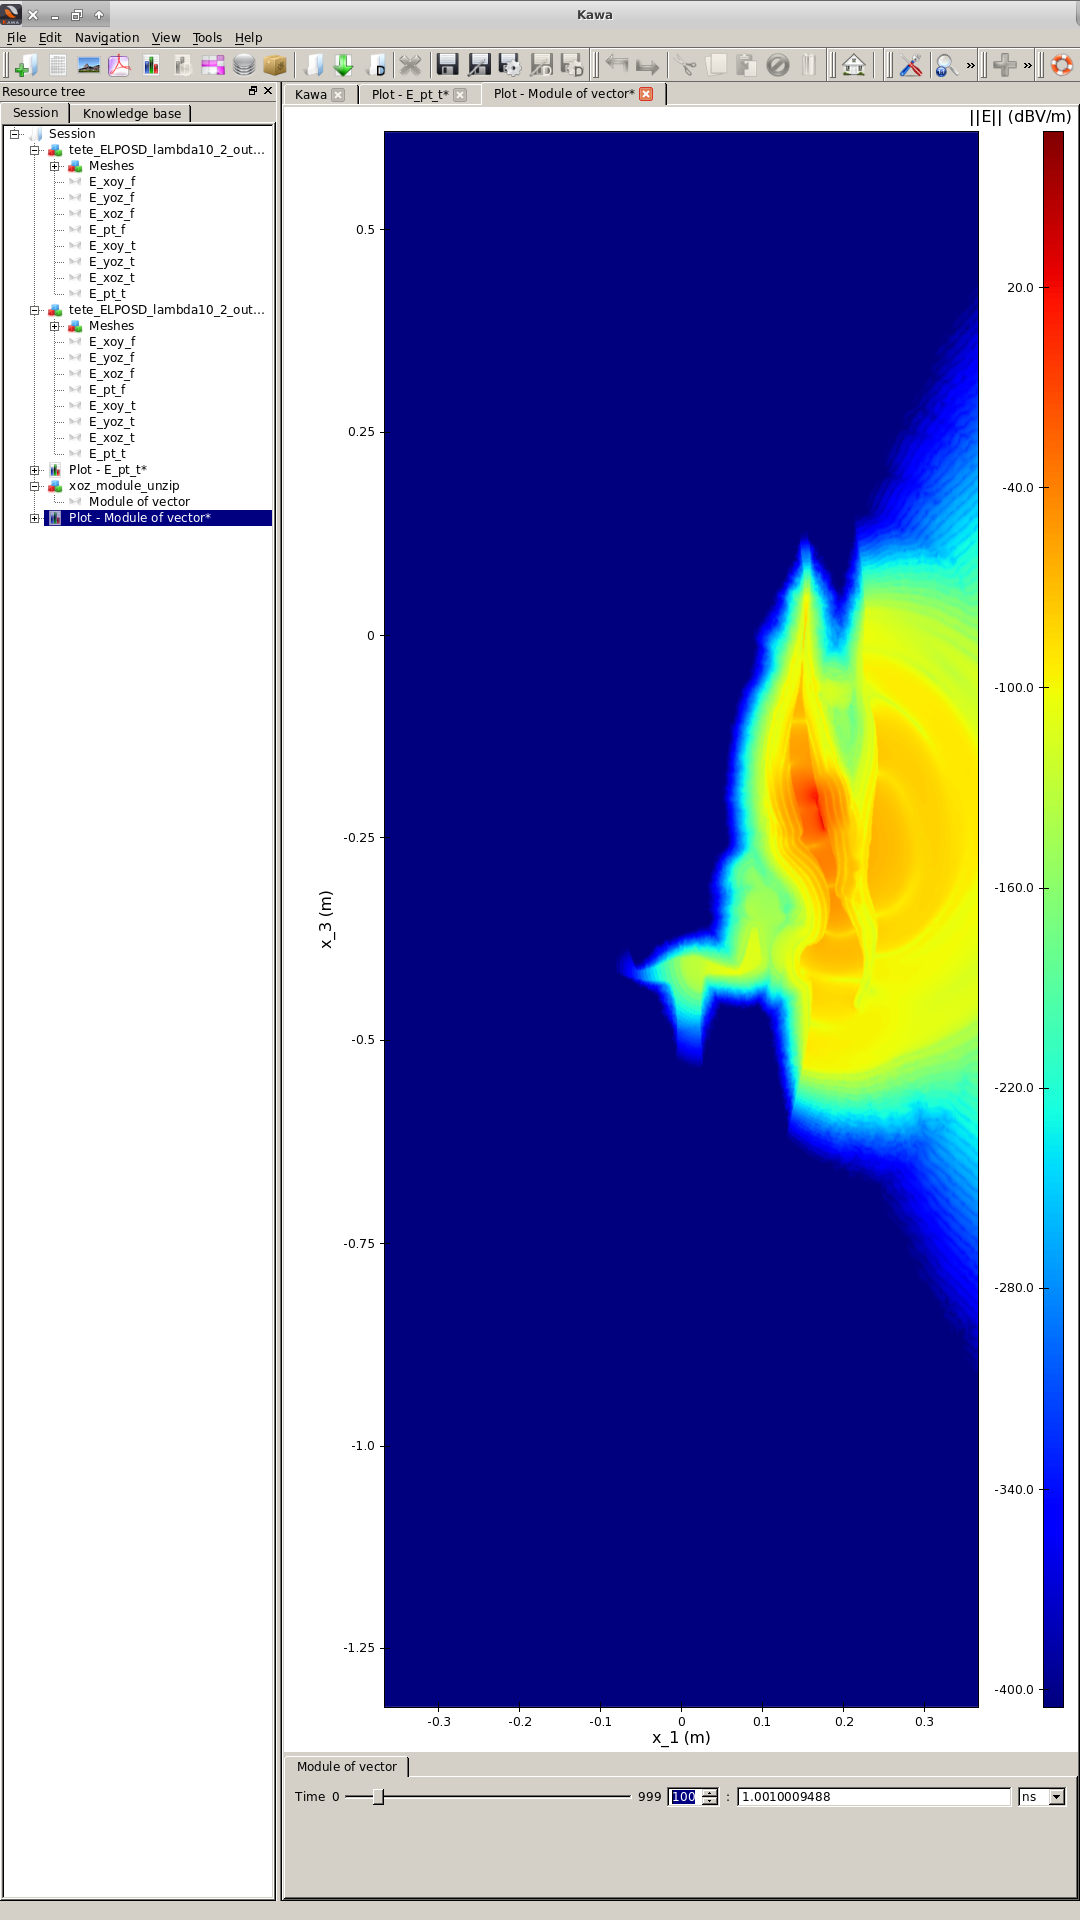
\includegraphics[
		width=0.66\linewidth,
		trim={317 170 8 108},clip
	]{kyoto_1ns}
\end{figure}

\begin{figure}[!h]
	\centering
	\caption{
		\label{img:annexe_kyoto_cutplane_2ns}
		Résultats en plan de coupe $(\x_1 O \x_3)$
		en $\x_2 = -0.1255$ m (antenne)
		au temps $t=2$ ns.
	}
	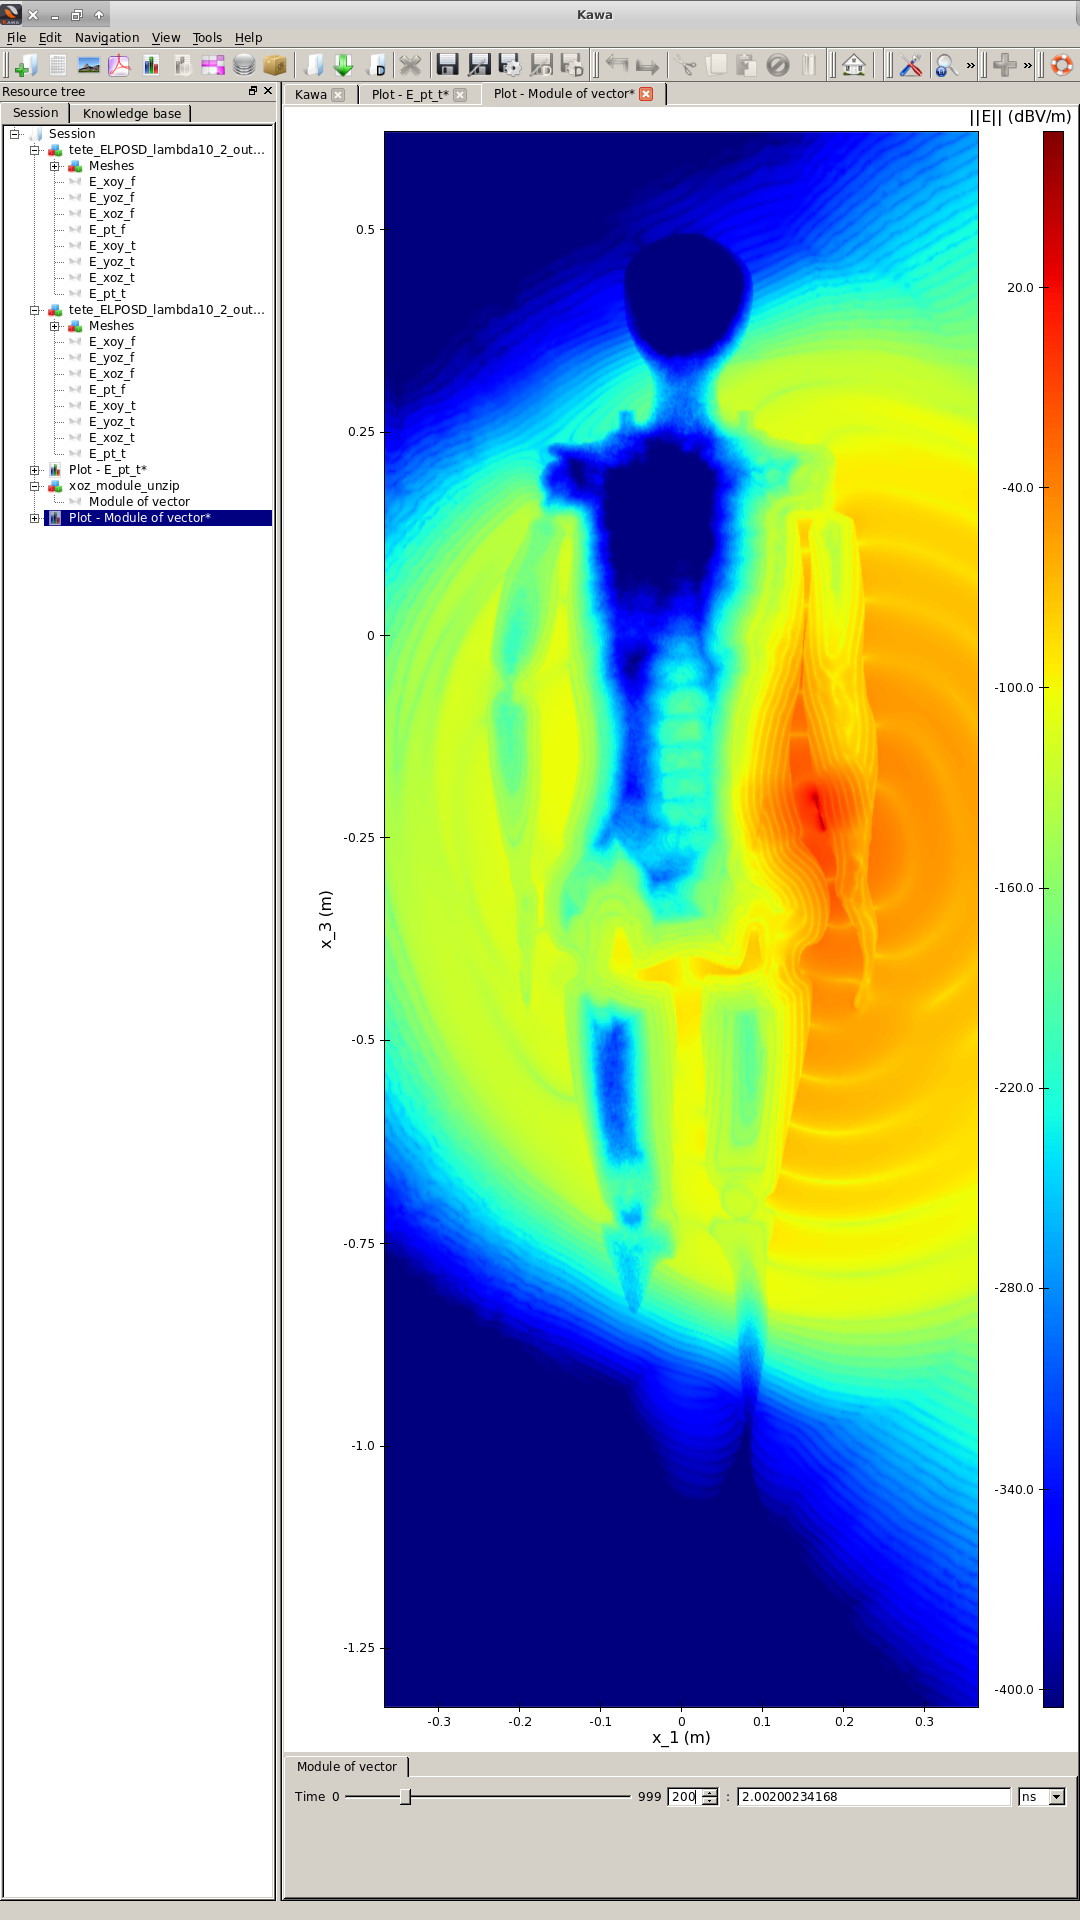
\includegraphics[
		width=0.66\linewidth,
		trim={317 170 8 108},clip
	]{kyoto_2ns}
\end{figure}

\begin{figure}[!h]
	\centering
	\caption{
		\label{img:annexe_kyoto_cutplane_3ns}
		Résultats en plan de coupe $(\x_1 O \x_3)$
		en $\x_2 = -0.1255$ m (antenne)
		au temps $t=3$ ns.
	}
	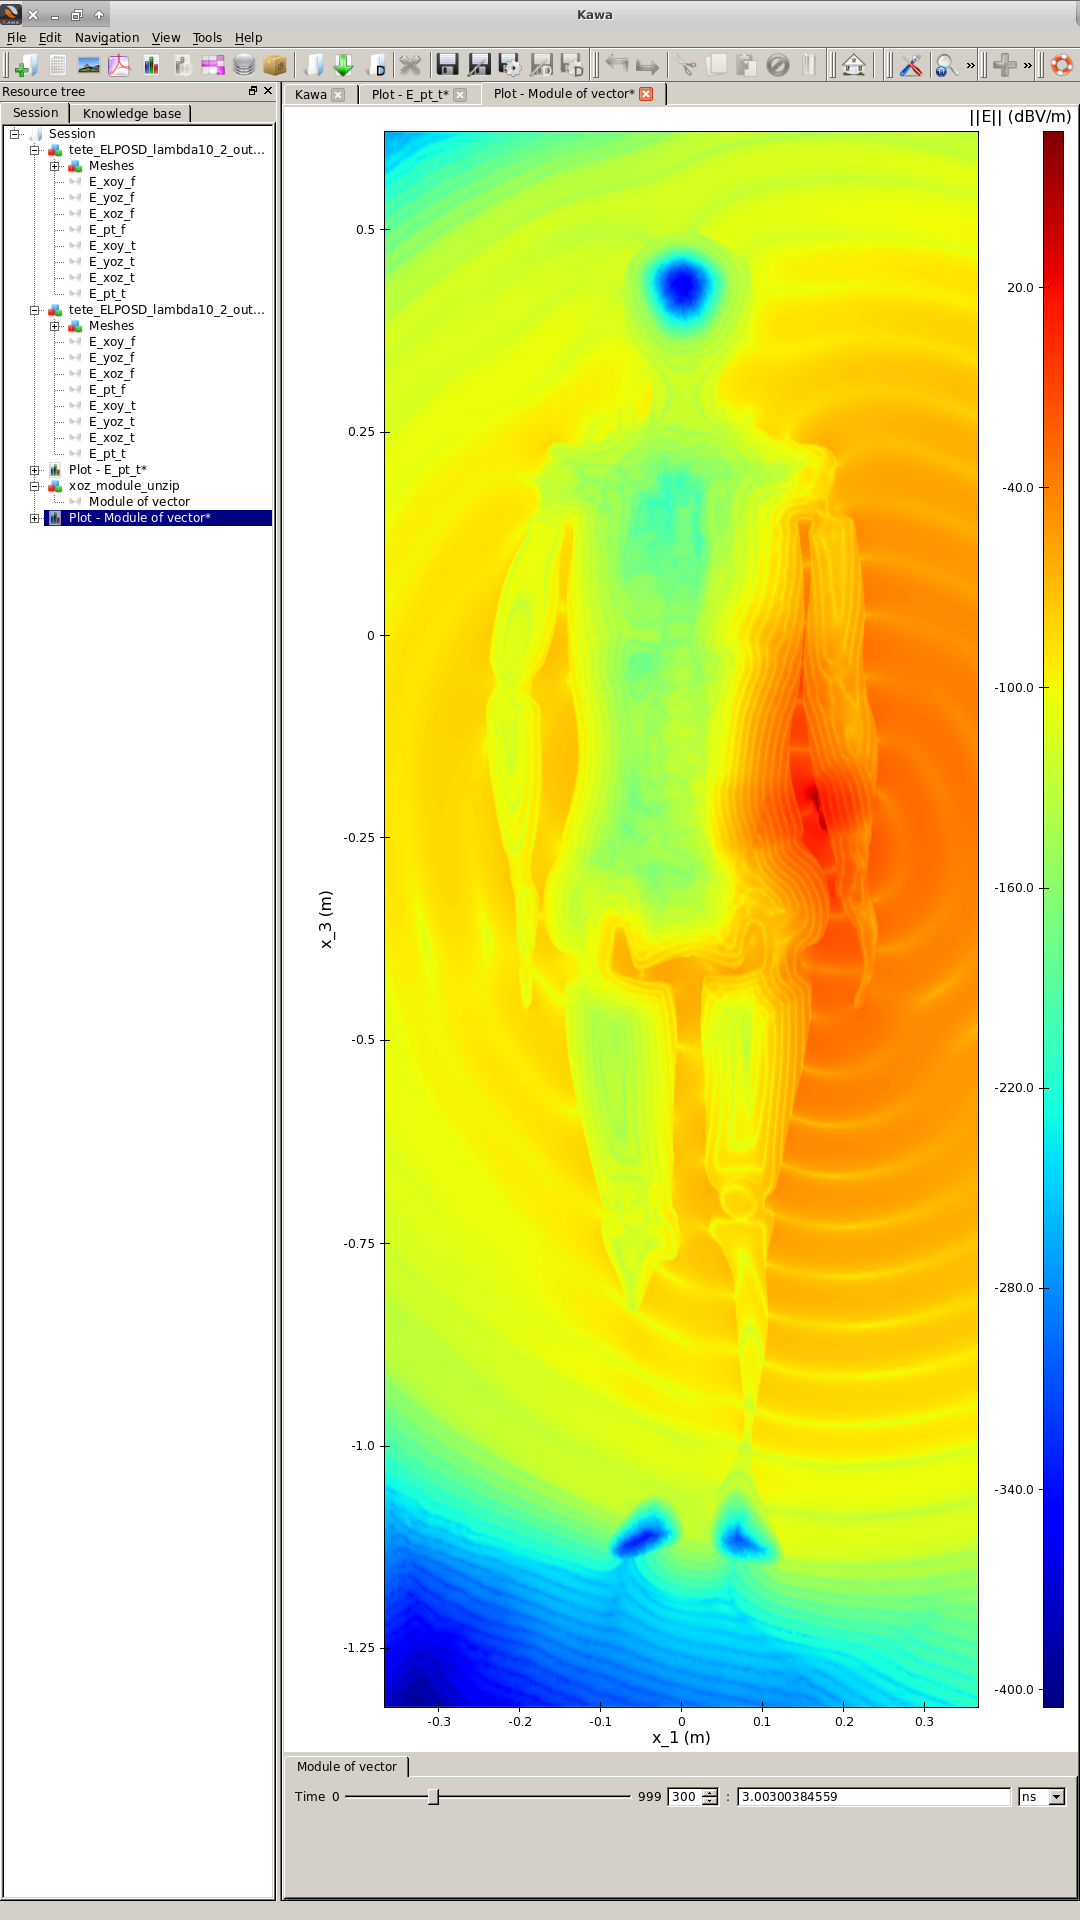
\includegraphics[
	width=0.66\linewidth,
	trim={317 170 8 108},clip
	]{kyoto_3ns}
\end{figure}

\begin{figure}[!h]
	\centering
	\caption{
		\label{img:annexe_kyoto_cutplane_4ns}
		Résultats en plan de coupe $(\x_1 O \x_3)$
		en $\x_2 = -0.1255$ m (antenne)
		au temps $t=4$ ns.
	}
	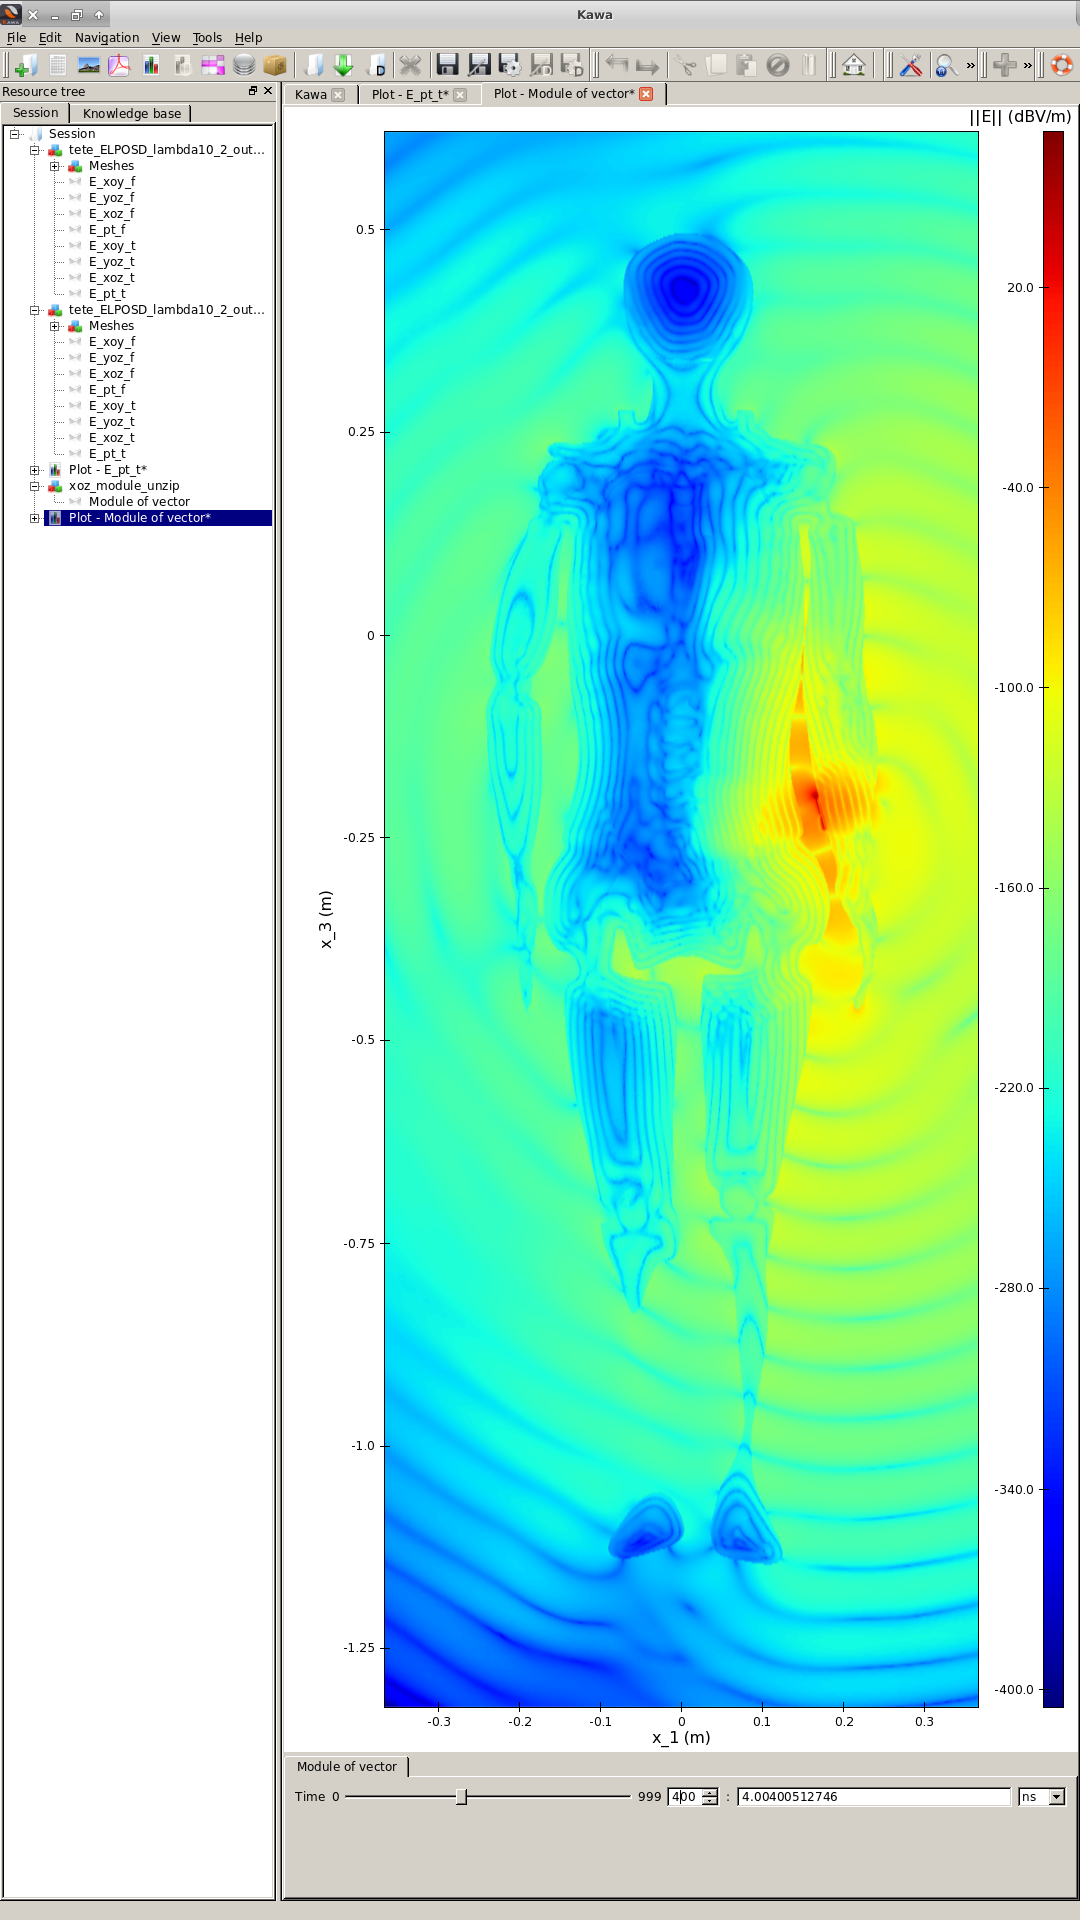
\includegraphics[
	width=0.66\linewidth,
	trim={317 170 8 108},clip
	]{kyoto_4ns}
\end{figure}

\begin{figure}[!h]
	\centering
	\caption{
		\label{img:annexe_kyoto_cutplane_5ns}
		Résultats en plan de coupe $(\x_1 O \x_3)$
		en $\x_2 = -0.1255$ m (antenne)
		au temps $t=5$ ns.
	}
	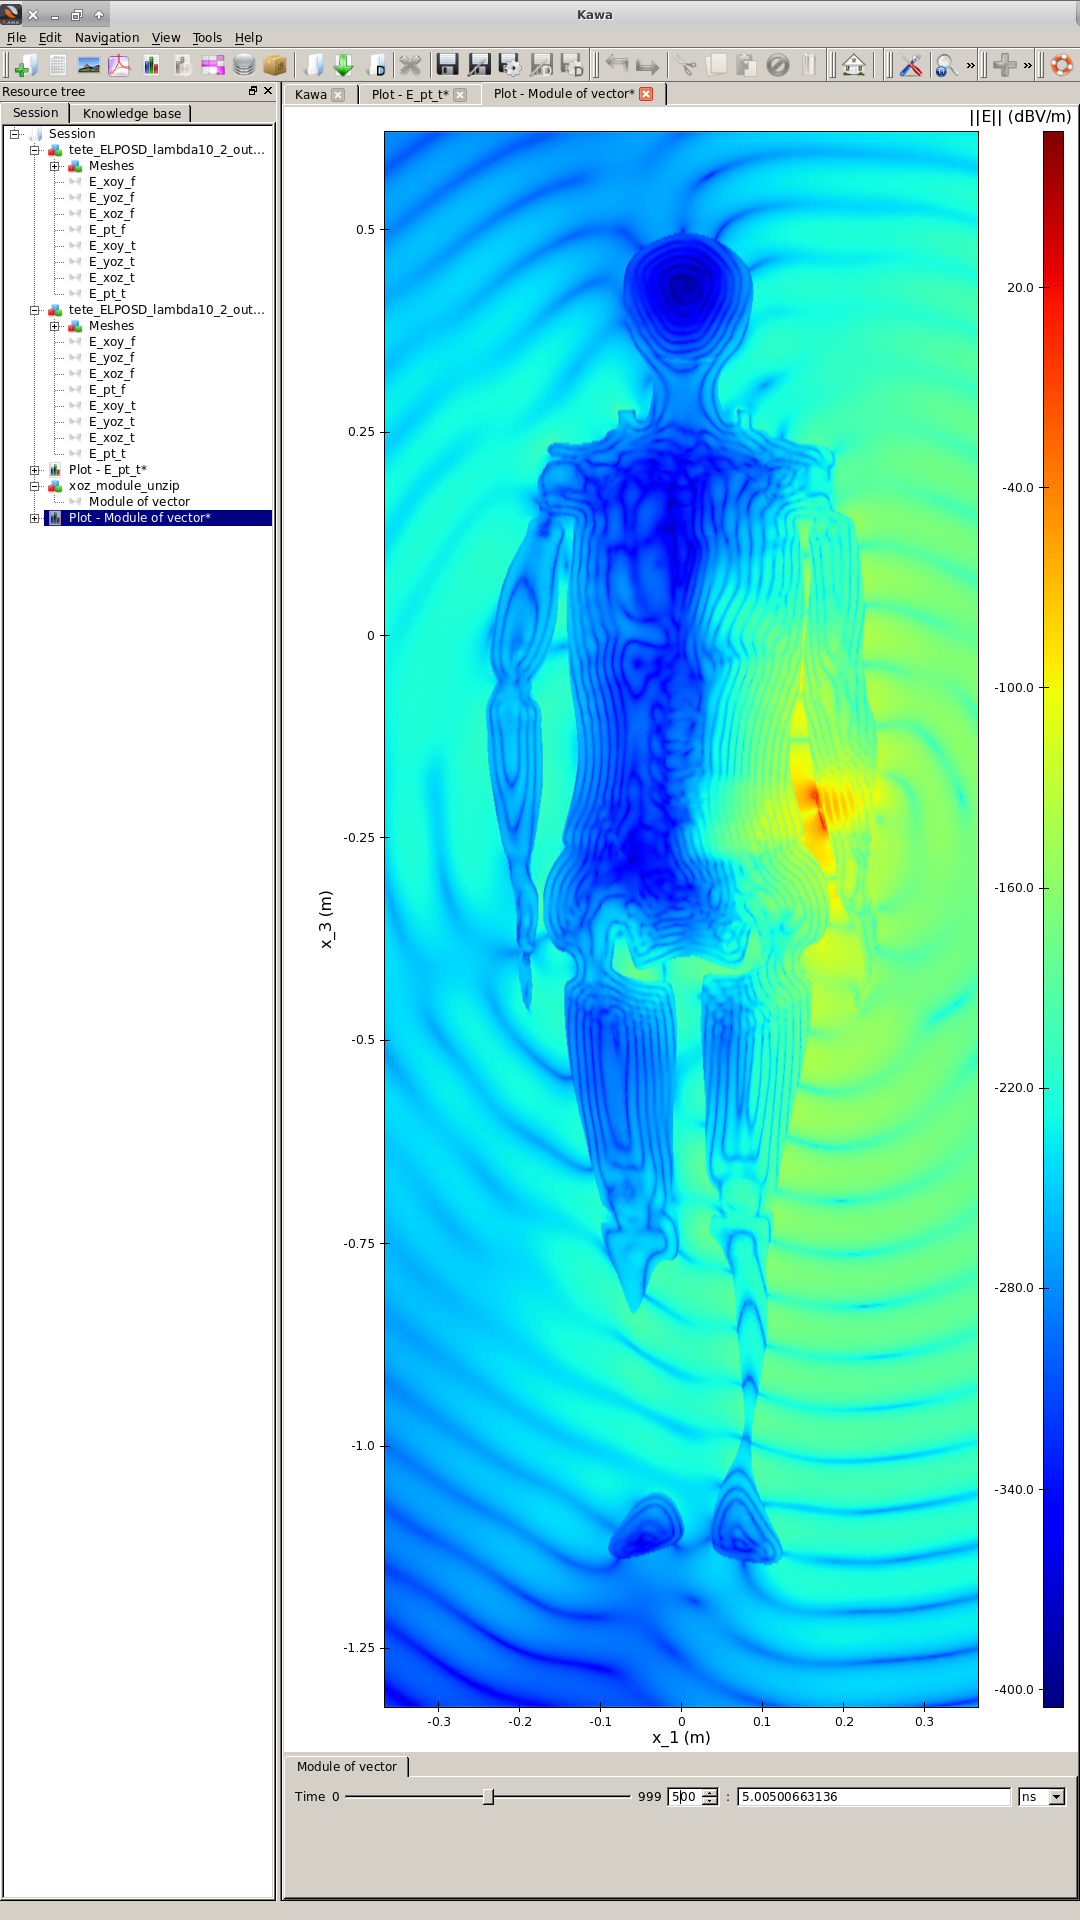
\includegraphics[
	width=0.66\linewidth,
	trim={317 170 8 108},clip
	]{kyoto_5ns}
\end{figure}

\begin{figure}[!h]
	\centering
	\caption{
		\label{img:annexe_kyoto_cutplane_6ns}
		Résultats en plan de coupe $(\x_1 O \x_3)$
		en $\x_2 = -0.1255$ m (antenne)
		au temps $t=6$ ns.
	}
	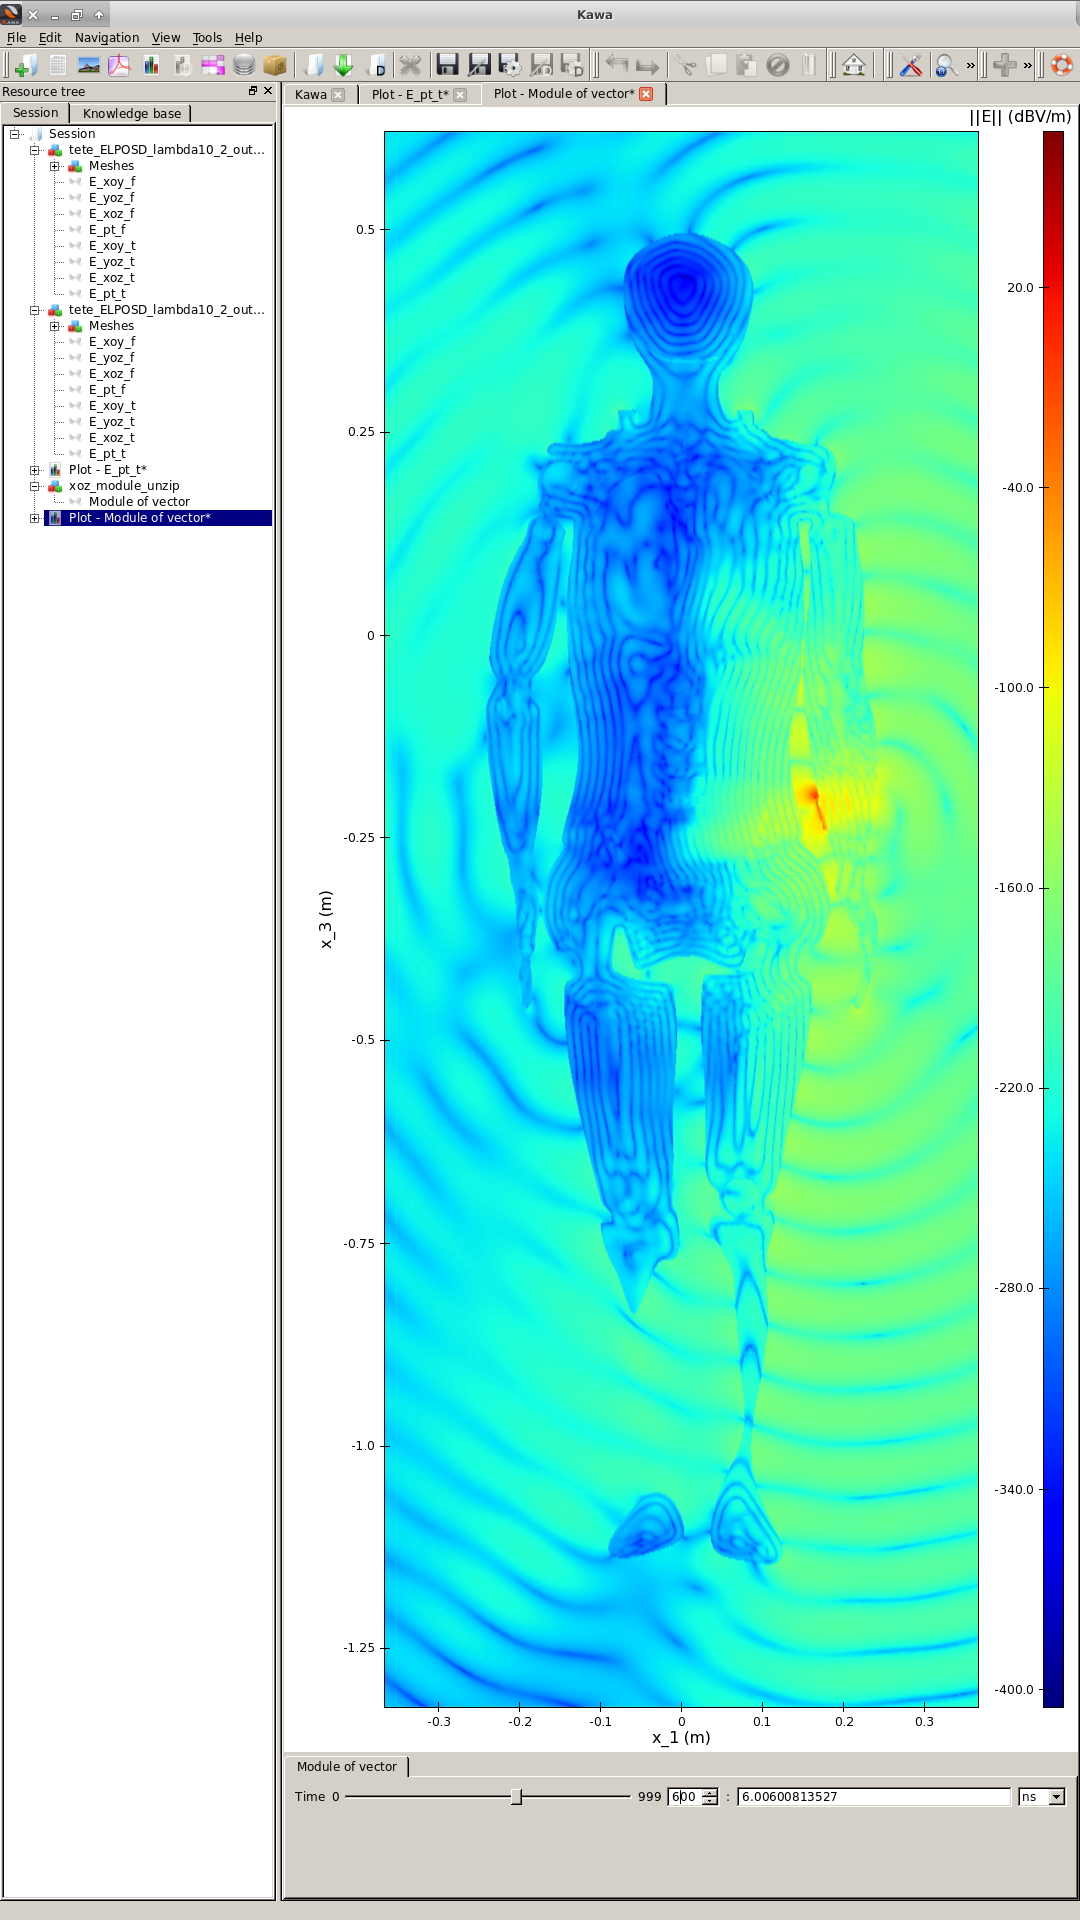
\includegraphics[
	width=0.66\linewidth,
	trim={317 170 8 108},clip
	]{kyoto_6ns}
\end{figure}

\begin{figure}[!h]
	\centering
	\caption{
		\label{img:annexe_kyoto_cutplane_7ns}
		Résultats en plan de coupe $(\x_1 O \x_3)$
		en $\x_2 = -0.1255$ m (antenne)
		au temps $t=7$ ns.
	}
	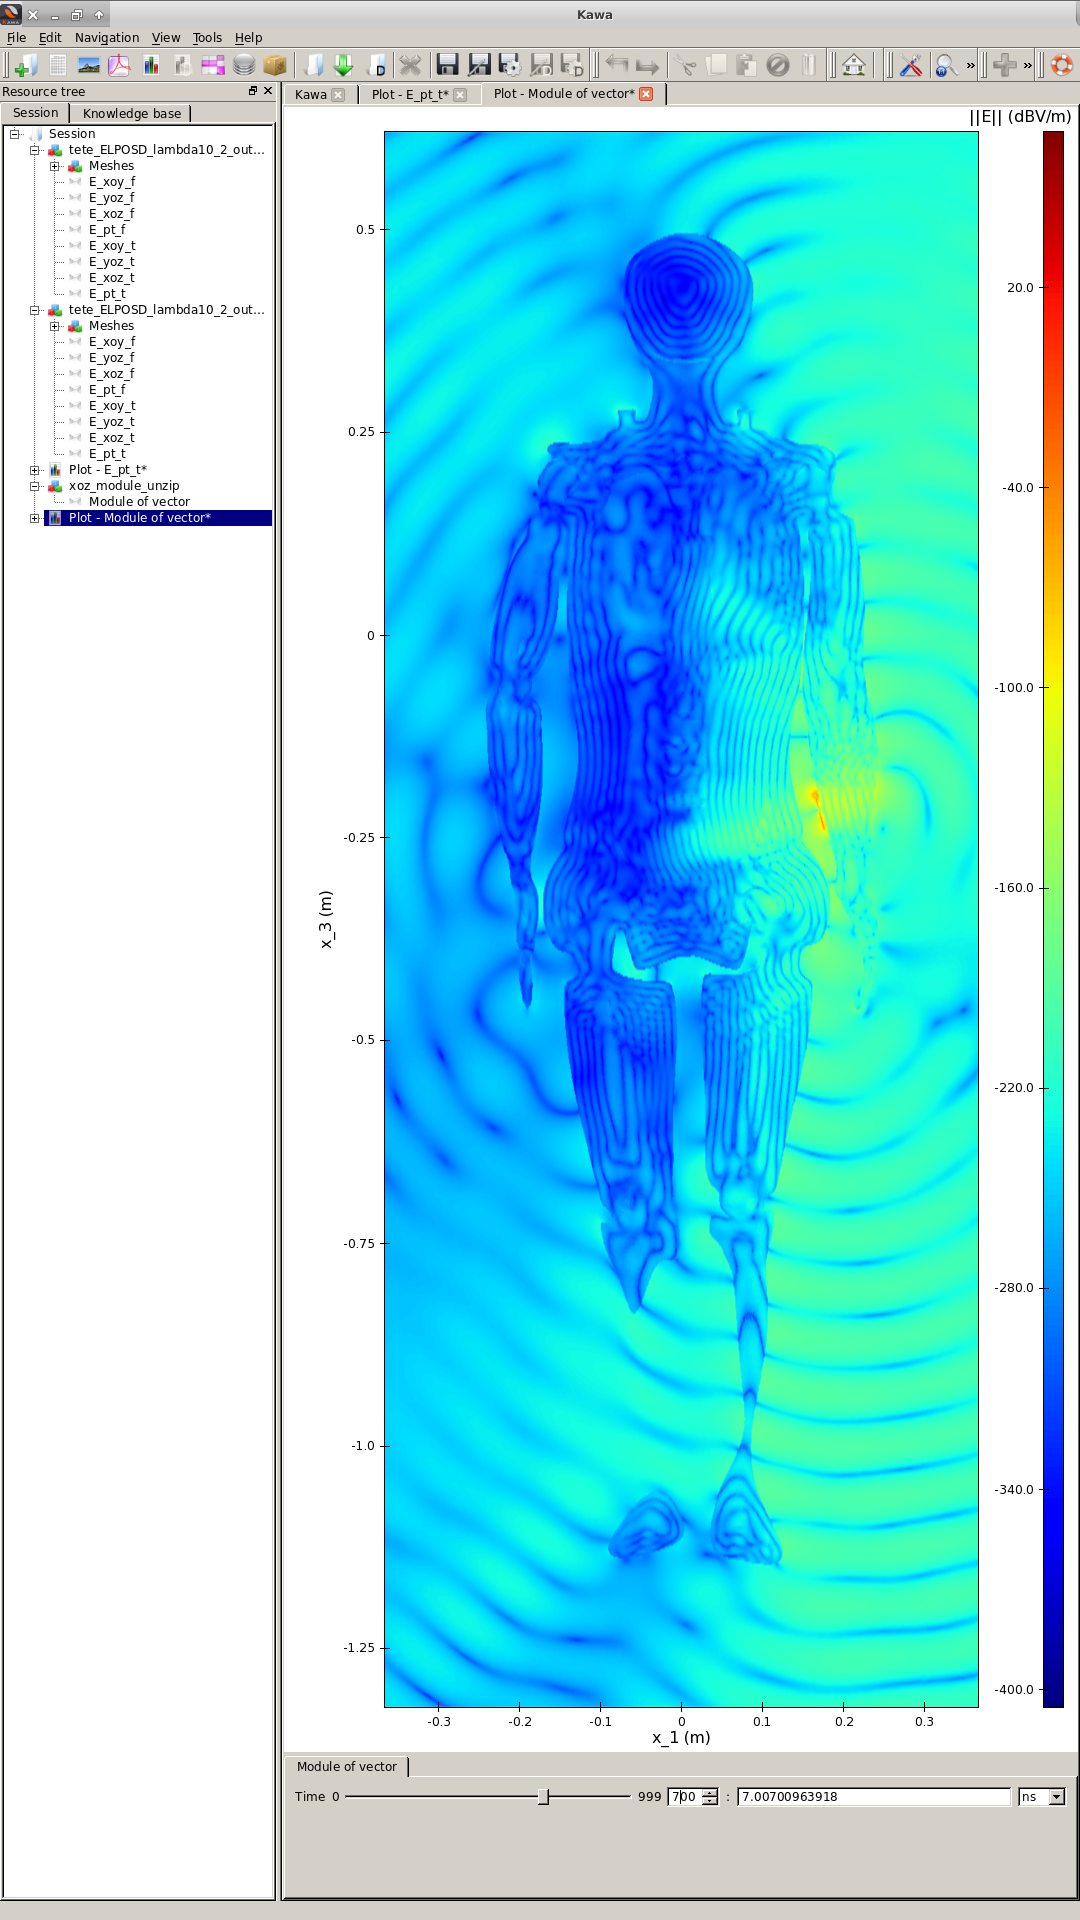
\includegraphics[
	width=0.66\linewidth,
	trim={317 170 8 108},clip
	]{kyoto_7ns}
\end{figure}

\begin{figure}[!h]
	\centering
	\caption{
		\label{img:annexe_kyoto_cutplane_8ns}
		Résultats en plan de coupe $(\x_1 O \x_3)$
		en $\x_2 = -0.1255$ m (antenne)
		au temps $t=8$ ns.
	}
	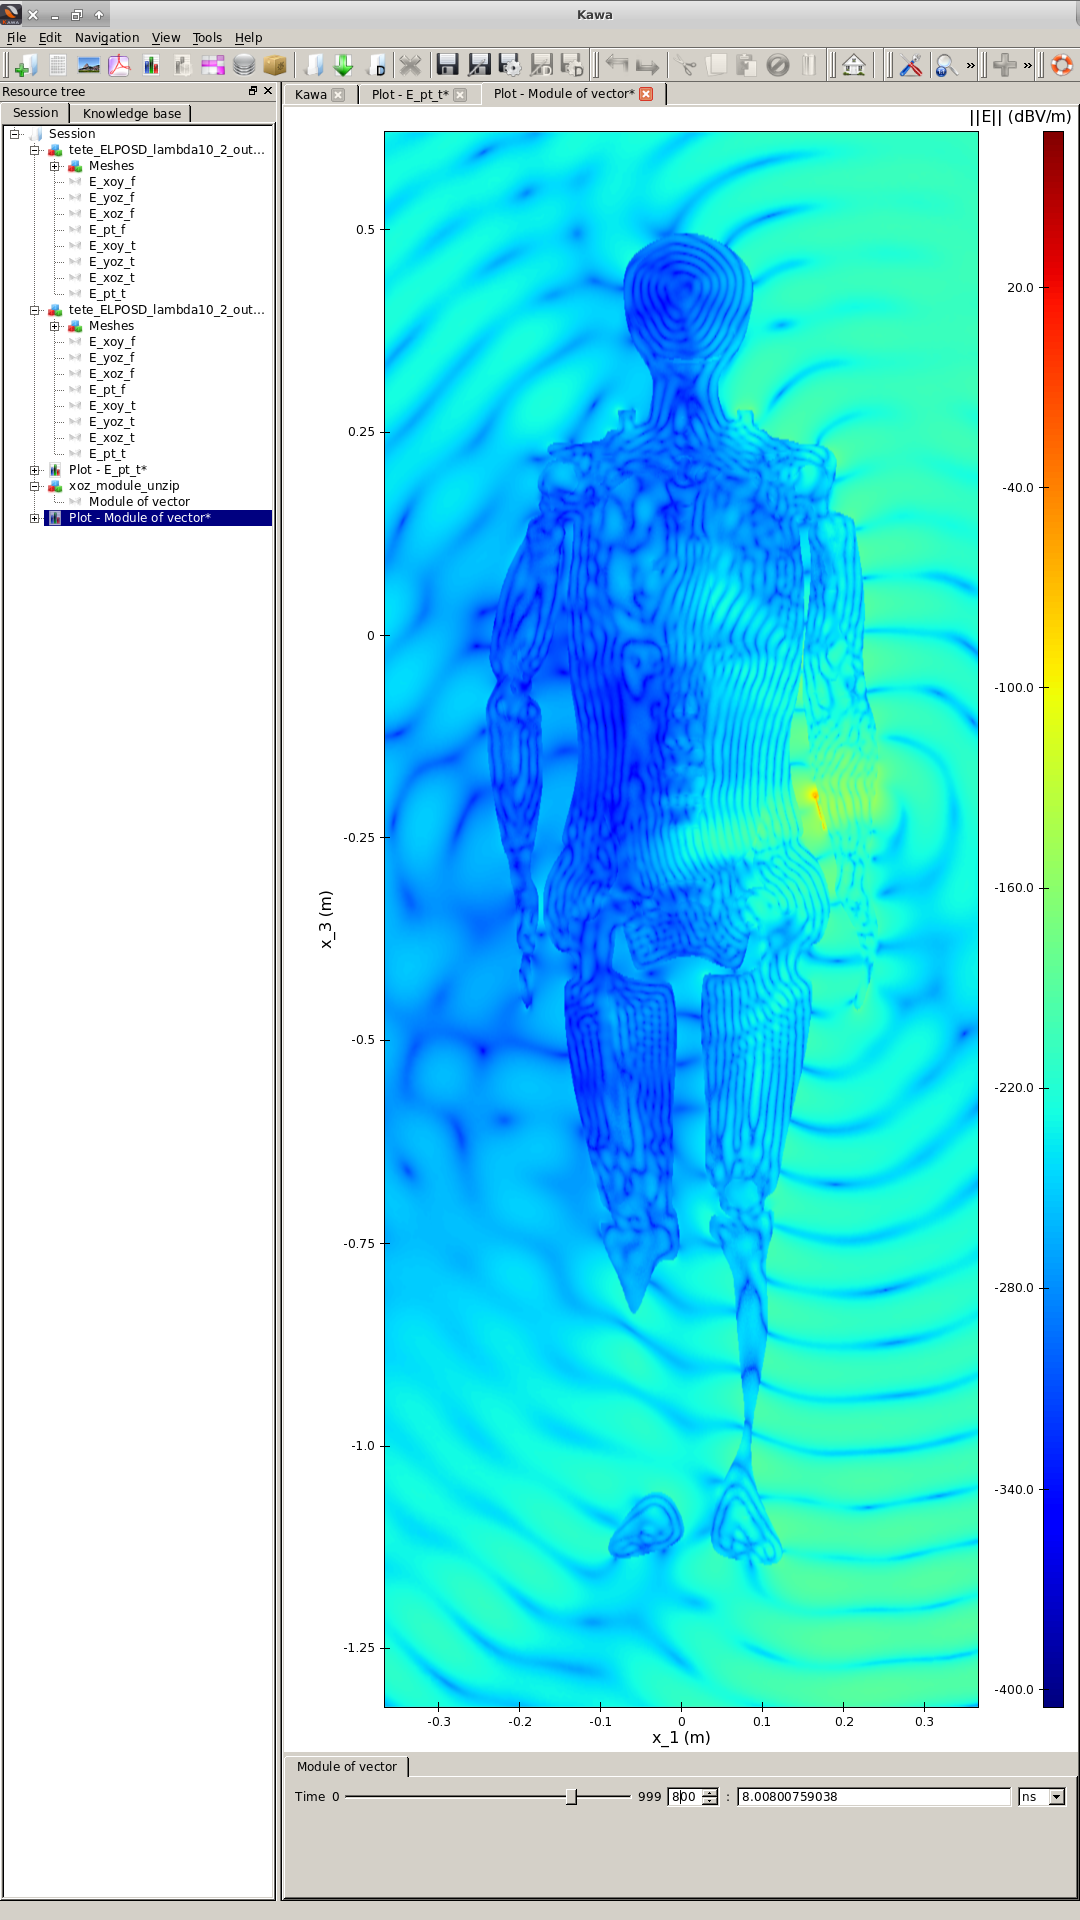
\includegraphics[
	width=0.66\linewidth,
	trim={317 170 8 108},clip
	]{kyoto_8ns}
\end{figure}

\begin{figure}[!h]
	\centering
	\caption{
		\label{img:annexe_kyoto_cutplane_9ns}
		Résultats en plan de coupe $(\x_1 O \x_3)$
		en $\x_2 = -0.1255$ m (antenne)
		au temps $t=9$ ns.
	}
	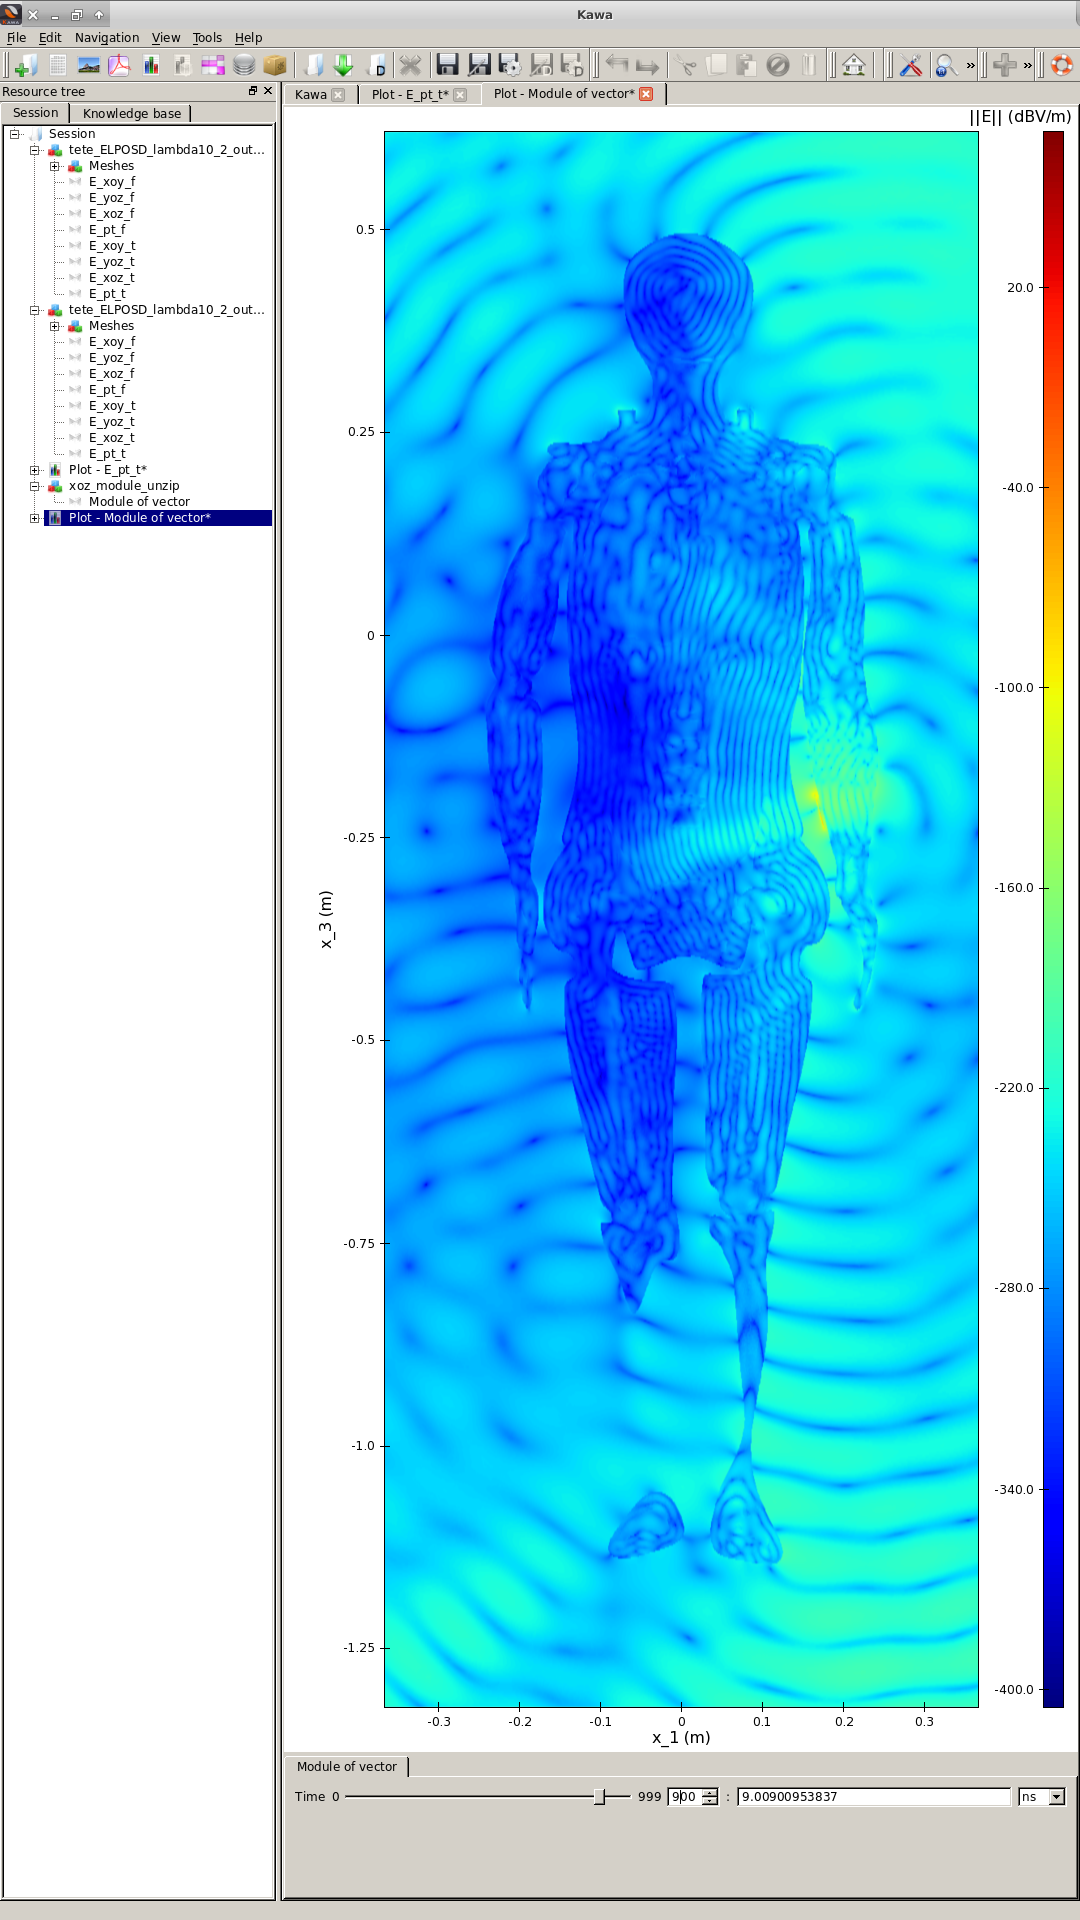
\includegraphics[
	width=0.66\linewidth,
	trim={317 170 8 108},clip
	]{kyoto_9ns}
\end{figure}

\begin{figure}[!h]
	\centering
	\caption{
		\label{img:annexe_kyoto_cutplane_10ns}
		Résultats en plan de coupe $(\x_1 O \x_3)$
		en $\x_2 = -0.1255$ m (antenne)
		au temps $t=10$ ns.
	}
	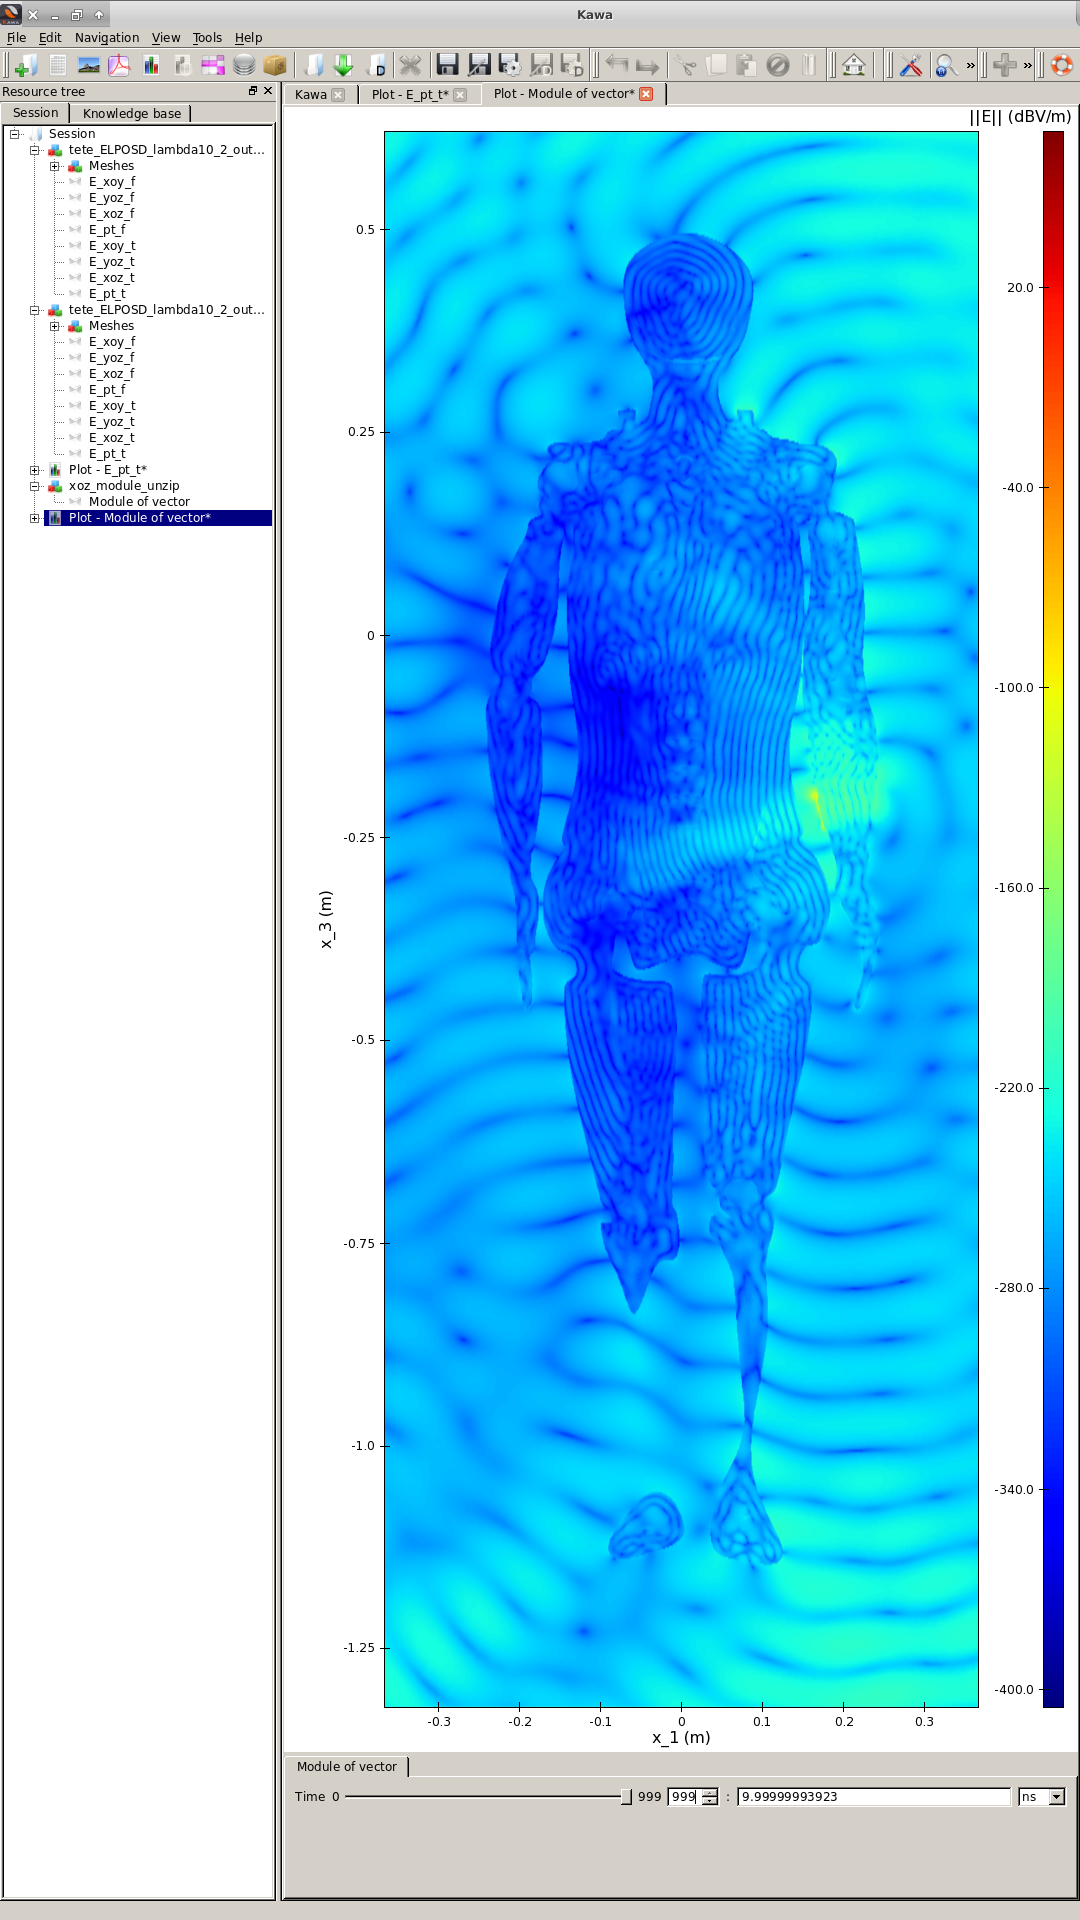
\includegraphics[
	width=0.66\linewidth,
	trim={317 170 8 108},clip
	]{kyoto_10ns}
\end{figure}



% Biblio
\cleardoublepage
\bibliographystyle{plain}
\bibliography{biblio}

\cleardoublepage
\thispagestyle{empty}
\hbox{}\newpage%\clearpage
\includepdf{4eme.pdf}

\end{document}
